% LaTeX source for ``Think Python: How to Think Like a Computer Scientist''
% Copyright (c)  2015  Allen B. Downey.

% License: Creative Commons Attribution-NonCommercial 3.0 Unported License.
% http://creativecommons.org/licenses/by-nc/3.0/
% Traduzione italiana di Andrea Zanella andreazanella@tiscali.it

%\documentclass[10pt,b5paper]{book}
\documentclass[10pt]{book}
\usepackage[width=5.5in,height=8.5in,hmarginratio=3:2,vmarginratio=1:1]{geometry}

% for some of these packages, you might have to install
% texlive-latex-extra (in Ubuntu)

\usepackage[T1]{fontenc}
\usepackage{textcomp}
\usepackage{mathpazo}
\usepackage{url}
\usepackage{fancyhdr}
\usepackage{graphicx}
\usepackage{amsmath}
\usepackage{amsthm}
\usepackage{amssymb}
\usepackage{exercise}                        % texlive-latex-extra
\usepackage{makeidx}
\usepackage{setspace}
\usepackage{hevea}                           
\usepackage{upquote}
\usepackage{appendix}
\usepackage[italian]{babel}
\usepackage[utf8x]{inputenc}
\usepackage{latexsym}
\usepackage[bookmarks]{hyperref}

\title{Pensare in Python}
\author{Allen B. Downey}
\newcommand{\thetitle}{Pensare in Python: Come pensare da Informatico}
\newcommand{\theversion}{Seconda Edizione, Versione 2.2.23}
\newcommand{\thedate}{}

% these styles get translated in CSS for the HTML version
\newstyle{a:link}{color:black;}
\newstyle{p+p}{margin-top:1em;margin-bottom:1em}
\newstyle{img}{border:0px}

% change the arrows
\setlinkstext
  {\imgsrc[ALT="Previous"]{back.png}}
  {\imgsrc[ALT="Up"]{up.png}}
  {\imgsrc[ALT="Next"]{next.png}}

\makeindex

\newif\ifplastex
\plastexfalse

\begin{document}

\frontmatter

% PLASTEX ONLY
\ifplastex
    \usepackage{localdef}
    \maketitle

\newcount\anchorcnt
\newcommand*{\Anchor}[1]{%
  \@bsphack%
    \Hy@GlobalStepCount\anchorcnt%
    \edef\@currentHref{anchor.\the\anchorcnt}% 
    \Hy@raisedlink{\hyper@anchorstart{\@currentHref}\hyper@anchorend}% 
    \M@gettitle{}\label{#1}% 
    \@esphack%
}


\else
% skip the following for plastex

\newtheorem{exercise}{Esercizio}[chapter]

% LATEXONLY

\input{latexonly}

\begin{latexonly}

\renewcommand{\blankpage}{\thispagestyle{empty} \quad \newpage}

%\blankpage
%\blankpage

% TITLE PAGES FOR LATEX VERSION

%-half title--------------------------------------------------
\thispagestyle{empty}

\begin{flushright}
\vspace*{2.0in}

\begin{spacing}{3}
{\huge Pensare in Python}\\
{\Large Come pensare da Informatico}
\end{spacing}

\vspace{0.25in}

\theversion

\thedate

\vfill

\end{flushright}

%--verso------------------------------------------------------

\blankpage
\blankpage
%\clearemptydoublepage
%\pagebreak
%\thispagestyle{empty}
%\vspace*{6in}

%--title page--------------------------------------------------
\pagebreak
\thispagestyle{empty}

\begin{flushright}
\vspace*{2.0in}

\begin{spacing}{3}
{\huge Pensare in Python}\\
{\Large Come pensare da Informatico}
\end{spacing}

\vspace{0.25in}

\theversion

\thedate

\vspace{1in}


{\Large
Allen Downey\\
}


\vspace{0.5in}

{\Large Green Tea Press}

{\small Needham, Massachusetts}

%\includegraphics[width=1in]{figs/logo1.pdf}
\vfill

\end{flushright}


%--copyright--------------------------------------------------
\pagebreak
\thispagestyle{empty}

{\small
Copyright \copyright ~2015 Allen Downey.


\vspace{0.2in}

\begin{flushleft}
Green Tea Press       \\
9 Washburn Ave        \\
Needham MA 02492
\end{flushleft}

È concessa l'autorizzazione a copiare, distribuire e/o modificare questo documento sotto i termini della Creative Commons Attribution-NonCommercial 3.0 Unported License, che è scaricabile dal sito \url{http://creativecommons.org/licenses/by-nc/3.0/}.

La forma originale di questo libro è in codice sorgente \LaTeX\ . La compilazione del sorgente \LaTeX\ ha l'effetto di generare una rappresentazione di un testo indipendente dal dispositivo, che può essere successivamente convertito in altri formati e stampato.

Il codice sorgente \LaTeX\ di questo libro è disponibile all'indirizzo
\url{http://www.thinkpython2.com}.

\vspace{0.2in}
Titolo originale: {\em Think Python: How to Think Like a Computer Scientist}.

Traduzione di Andrea Zanella.


\vspace{0.2in}

} % end small

\end{latexonly}


% HTMLONLY

\begin{htmlonly}

% TITLE PAGE FOR HTML VERSION

{\Large \thetitle}

{\large Allen B. Downey}

\theversion

\thedate

\setcounter{chapter}{-1}

\end{htmlonly}

\fi
% END OF THE PART WE SKIP FOR PLASTEX


\chapter{Prefazione}

\section*{La strana storia di questo libro}

Nel gennaio 1999 mi stavo preparando a tenere un corso introduttivo di programmazione in Java. Lo avevo tenuto già tre volte, ma ne stavo diventando sempre più insoddisfatto. Il tasso di insuccesso nel corso era troppo elevato, e anche per gli studenti che venivano promossi, il livello globale di apprendimento era troppo basso.

Uno dei problemi che avevo individuato erano i libri. Troppo grandi, con troppi dettagli non necessari su Java e privi di una guida di alto livello su come programmare. E tutti soffrivano dell' ``effetto botola'': cominciavano in modo semplice, procedevano gradualmente e poi, verso il Capitolo 5, mancava il pavimento sotto i piedi. Gli studenti si trovavano con troppo nuovo materiale e troppo velocemente, e io passavo il resto del semestre a raccogliere i cocci.

Due settimane prima dell'inizio delle lezioni, decisi allora di scrivere un libro tutto mio. I miei obiettivi erano:

\begin{itemize}

\item Mantenerlo breve. Gli studenti preferiscono leggere 10 pagine piuttosto che 50.

\item Prestare attenzione ai vocaboli. Cercai di ridurre al minimo i termini gergali e di spiegare ciascun termine la prima volta che veniva usato.

\item Costruire gradualmente. Per evitare le ``botole'', presi gli argomenti più ostici suddividendoli in una serie di piccoli passi.

\item Focalizzare sulla programmazione, non sul linguaggio di programmazione. Inclusi la minima parte necessaria di Java e tralasciai il resto.

\end{itemize}

Mi serviva un titolo, così d'istinto scelsi {\em Come pensare da Informatico}.

La prima versione era grezza, ma funzionò. Gli studenti lo lessero, e capirono abbastanza da permettermi di impiegare il tempo della lezione per gli argomenti più difficili, per quelli interessanti e (cosa più importante) per la parte pratica.

Pubblicai il libro sotto la GNU Free Documentation License, che permette ai fruitori di copiare, modificare, e distribuire il libro.

\index{GNU Free Documentation License}
\index{Free Documentation License, GNU}

Ma il bello venne dopo. Jeff Elkner, insegnante di liceo in Virginia, utilizzò il mio libro adattandolo per Python. Mi mandò una copia della sua versione, e io ebbi la insolita esperienza di imparare Python leggendo il mio stesso libro. Con la Green Tea Press, pubblicai la prima versione Python nel 2001.
\index{Elkner, Jeff}

Nel 2003 cominciai a lavorare all'Olin College, ed ottenni di insegnare Python per la prima volta. Il contrasto con Java fu abissale. Gli studenti dovettero faticare meno, impararono di più, lavorarono su progetti più interessanti, e in generale si divertirono di più.
\index{Olin College}

Da allora, ho continuato a sviluppare il libro, correggendo errori, migliorando alcuni esempi e aggiungendo nuovo materiale, soprattutto esercizi.

Il risultato è questo libro, che ora ha il meno grandioso titolo 
{\em Pensare in Python}.  Ecco alcune novità:

\begin{itemize}

\item Ho aggiunto un paragrafo sul debug alla fine di ciascun capitolo. Questi paragrafi presentano le tecniche generali per scovare ed evitare gli errori, e le avvertenze sui trabocchetti di Python.

\item Ho aggiunto altri esercizi, da brevi test di apprendimento ad alcuni progetti sostanziosi. Per la maggior parte di essi, c'è un collegamento web alla soluzione.

\item Ho aggiunto una serie di esercitazioni - esempi più articolati con esercizi, soluzioni e discussione. 
  
\item Ho ampliato la trattazione sui metodi di sviluppo di un programma e sugli schemi fondamentali di progettazione.

\item Ho aggiunto delle appendici sul debug e l'analisi degli algoritmi.

\end{itemize}

Novità di questa seconda edizione:

\begin{itemize}

\item Il libro e tutto il codice di supporto sono stati aggiornati a Python 3.

\item Ho aggiunto alcuni paragrafi, con ulteriori dettagli sul web, per aiutare i meno esperti ad iniziare a usare Python in un browser, in modo da non doverne affrontare l'installazione fino a quando non si sentiranno pronti.

\item Per il capitolo~\ref{turtlechap}, al posto del mio pacchetto grafico basato su {\em turtle graphics}, chiamato Swampy, ho adottato il modulo {\em turtle} di Python, più standard, potente e facile da installare.

\item Ho inserito un nuovo capitolo chiamato ``Ulteriori strumenti'', che presenta alcune funzionalità aggiuntive di Python non indispensabili, ma che possono tornare utili.

\end{itemize}

Spero che troviate piacevole utilizzare questo libro, e che vi aiuti, almeno un pochino, ad imparare a programmare e a pensare da informatici.


Allen B. Downey \\

Olin College\\


\section*{Ringraziamenti}

Grazie infinite a Jeff Elkner, che ha adattato a Python il mio libro su Java, ha dato inizio a questo progetto e mi ha introdotto in quello che poi è diventato il mio linguaggio di programmazione preferito. 
\index{Elkner, Jeff}

Grazie anche a Chris Meyers, che ha contribuito ad alcuni paragrafi di
{\em How to Think Like a Computer Scientist}.
\index{Meyers, Chris}

Grazie alla Free Software Foundation per aver sviluppato la GNU Free Documentation License, che ha aiutato a rendere possibile la mia collaborazione con Jeff e Chris, e a Creative Commons per la licenza che uso attualmente.
\index{GNU Free Documentation License}
\index{Free Documentation License, GNU}
\index{Creative Commons}

Grazie ai redattori di Lulu che hanno lavorato a
{\em How to Think Like a Computer Scientist}.

Grazie ai redattori di O'Reilly Media che hanno lavorato a
{\em Think Python}.

Grazie a tutti gli studenti che hanno usato le versioni precedenti di questo libro e a tutti coloro (elencati di seguito) che hanno contribuito inviando correzioni e suggerimenti.


\section*{Elenco dei collaboratori}

\index{collaboratori}
Più di 100 lettori premurosi e dalla vista aguzza hanno inviato suggerimenti e correzioni negli anni passati. Il loro contributo e l'entusiasmo per questo progetto, sono stati di enorme aiuto.

Se volete proporre suggerimenti o correzioni, inviate una email a 
{\tt feedback@thinkpython.com}. Se farò delle modifiche in seguito al vostro contributo, sarete aggiunti all'elenco dei collaboratori (a meno che non chiediate di non comparire).

Se includete almeno parte della frase in cui si trova l'errore, mi faciliterete la ricerca. Vanno bene anche numeri di pagina e di paragrafo, ma sono meno agevoli da trattare. Grazie!

\begin{itemize}

\small
\item Lloyd Hugh Allen ha inviato una correzione al Paragrafo 8.4.

\item Yvon Boulianne ha inviato una correzione a un errore di semantica nel Capitolo 5.

\item Fred Bremmer ha inviato una correzione al Paragrafo 2.1.

\item Jonah Cohen ha scritto gli script Perl per convertire i sorgenti
LaTeX di questo libro in un meraviglioso HTML.

\item Michael Conlon ha inviato una correzione grammaticale nel Capitolo 2
e un miglioramento dello stile nel Capitolo 1, e ha iniziato la discussione sugli aspetti tecnici degli interpreti.

\item Benoit Girard ha inviato una correzione ad un umoristico errore nel Paragrafo 5.6.

\item Courtney Gleason e Katherine Smith hanno scritto {\tt horsebet.py},
che veniva usato come esercitazione in una versione precedente del libro. Ora il loro programma si può trovare sul sito web.

\item Lee Harr ha sottoposto più correzioni di quelle che è possibile elencare in questo spazio, e pertanto andrebbe considerato come uno dei principali revisori del testo.

\item James Kaylin è uno studente che ha usato il libro. Ha sottoposto numerose correzioni.

\item David Kershaw ha sistemato la funzione errata {\tt catTwice} nel Paragrafo
3.10.

\item Eddie Lam ha mandato molte correzioni ai Capitoli 1, 2, e 3.
Ha anche sistemato il Makefile in modo che crei un indice alla prima esecuzione e ha aiutato nell'impostazione dello schema delle versioni.  

\item Man-Yong Lee ha inviato una correzione al codice di esempio nel Paragrafo 2.4.  

\item David Mayo ha puntualizzato che la parola ``inconsciamente' nel Capitolo 1 doveva essere cambiata in ``subconsciamente''.

\item Chris McAloon ha inviato alcune correzioni ai Paragrafi 3.9 e
3.10.

\item Matthew J. Moelter è un collaboratore di lunga data che ha inviato numerose correzioni e suggerimenti al libro.  

\item Simon Dicon Montford ha comunicato una definizione di funzione mancante e alcuni errori di battitura nel Capitolo 3. Ha anche trovato un errore nella funzione {\tt incremento} nel Capitolo 13.

\item John Ouzts ha corretto la definizione di ``valore di ritorno'' nel Capitolo 3.

\item Kevin Parks ha inviato preziosi commenti e suggerimenti su come migliorare la distribuzione del libro.

\item David Pool ha inviato un errore di battitura nel glossario del Capitolo 1, e gentili parole di incoraggiamento.

\item Michael Schmitt ha inviato correzioni al capitolo sui file e le eccezioni.

\item Robin Shaw ha evidenziato un errore nel Paragrafo 13.1 dove la funzione printTime veniva usata in un esempio senza essere definita.

\item Paul Sleigh ha trovato un errore nel Capitolo 7 e un bug nello script Perl di Jonah Cohen che genera HTML a partire da LaTeX.

\item Craig T. Snydal sta provando il testo in un corso presso la Drew
University. Ha contribuito con alcuni preziosi consigli e correzioni.

\item Ian Thomas e i suoi studenti stanno usando il testo in un corso di programmazione. Sono i primi a collaudare i capitoli della seconda metà del libro, e hanno apportato numerose correzioni e suggerimenti.

\item Keith Verheyden ha inviato una correzione al Capitolo 3.

\item Peter Winstanley ci ha portato a conoscenza di un annoso errore nel nostro carattere latin nel Capitolo 3.

\item Chris Wrobel ha apportato correzioni al codice nel capitolo su file I/O ed eccezioni. 

\item Moshe Zadka ha dato un inestimabile contributo a questo progetto. Oltre a scrivere la prima bozza del capitolo sui Dizionari, è stato una continua fonte di indicazioni nei primi abbozzi di questo libro.

\item Christoph Zwerschke ha inviato alcune correzioni e suggerimenti pedagogici, e ha spiegato la differenza tra {\em gleich} e {\em selbe}.

\item James Mayer ci ha mandato correzioni a un sacco di errori di battitura e di dizione, compresi due nell'elenco dei collaboratori.

\item Hayden McAfee ha colto una incongruenza, fonte di probabile confusione, tra due esempi.

\item Angel Arnal fa parte del gruppo internazionale di traduttori e lavora sulla versione spagnola. Ha trovato anche alcuni errori nella versione inglese.

\item Tauhidul Hoque e Lex Berezhny hanno creato le illustrazioni del Capitolo 1 e migliorato molte delle altre.

\item Il Dr. Michele Alzetta ha colto un errore nel Capitolo 8 e inviato alcuni interessanti commenti pedagogici su Fibonacci e Old Maid.

\item Andy Mitchell ha trovato un errore di battitura nel Capitolo1 e un esempio non funzionante nel Capitolo 2.

\item Kalin Harvey ha suggerito un chiarimento nel Capitolo 7 e ha trovato alcuni errori di battitura.

\item Christopher P. Smith ha trovato alcuni errori di battitura e ci ha aiutato ad aggiornare il libro a Python 2.2 .

\item David Hutchins ha trovato un errore di battitura nella Premessa.

\item Gregor Lingl insegna Python in un liceo di Vienna, in Austria. Sta lavorando alla traduzione tedesca del libro e ha trovato un paio di brutti errori nel Capitolo 5.

\item Julie Peters ha trovato un errore di battitura nella Premessa.

\item Florin Oprina ha inviato un miglioramento in {\tt makeTime},
una correzione in {\tt printTime}, e un simpatico errore di battitura.

\item D.~J.~Webre ha suggerito un chiarimento nel Capitolo 3.

\item Ken ha trovato una manciata di errori nei Capitoli 8, 9 e 11.

\item Ivo Wever ha trovato un errore di battitura nel Capitolo 5 e ha suggerito un chiarimento nel Capitolo 3.

\item Curtis Yanko ha suggerito un chiarimento nel Capitolo 2.

\item Ben Logan ha evidenziato alcuni errori di battitura e dei problemi nella trasposizione del libro in HTML.

\item Jason Armstrong ha notato una parola mancante nel Capitolo 2.

\item Louis Cordier ha notato un punto del Capitolo 16 dove il codice non corrispondeva al testo.

\item Brian Cain ha suggerito dei chiarimenti nei Capitoli 2 e 3.

\item Rob Black ha inviato un'ampia raccolta di correzioni, inclusi alcuni cambiamenti per Python 2.2.

\item Jean-Philippe Rey dell'Ecole Centrale di Parigi ha inviato un buon numero di correzioni, inclusi degli aggiornamenti per Python 2.2 e altri preziosi miglioramenti.

\item Jason Mader della George Washington University ha dato parecchi utili suggerimenti e correzioni.

\item Jan Gundtofte-Bruun ci ha ricordato che ``a error'' è un errore.

\item Abel David e Alexis Dinno ci hanno ricordato che il plurale di
``matrix'' è ``matrices'', non ``matrixes''.  Questo errore è rimasto nel libro per anni, ma due lettori con le stesse iniziali lo hanno segnalato nello stesso giorno. Curioso.

\item Charles Thayer ci ha spronati a sbarazzarci dei due punti che avevamo messo alla fine di alcune istruzioni, e a fare un uso più appropriato di ``argomenti'' e ``parametri''.

\item Roger Sperberg ha indicato un brano dalla logica contorta nel Capitolo 3.

\item Sam Bull ha evidenziato un paragrafo confuso nel Capitolo 2.

\item Andrew Cheung ha evidenziato due istanze di ``uso prima di def.''

\item C. Corey Capel ha notato una parola mancante nel Terzo Teorema del Debugging e un errore di battitura nel Capitolo 4.

\item Alessandra ha aiutato a sistemare un po' di confusione nelle Tartarughe.

\item Wim Champagne ha trovato un errore in un esempio di dizionario.

\item Douglas Wright ha trovato un problema con la divisione intera in
{\tt arco}.

\item Jared Spindor ha trovato alcuni scarti alla fine di una frase.

\item Lin Peiheng ha inviato una serie di suggerimenti molto utili.

\item Ray Hagtvedt ha sottoposto due errori e un non-abbastanza-errore.

\item Torsten H\"{u}bsch ha evidenziato un'incongruenza in Swampy.

\item Inga Petuhhov ha corretto un esempio nel Capitolo 14.

\item Arne Babenhauserheide ha inviato alcune utili correzioni.

\item Mark E. Casida è bravo bravo a trovare parole ripetute.

\item Scott Tyler ha inserito una che mancava. E ha poi inviato una pila di correzioni.

\item Gordon Shephard ha inviato alcune correzioni, tutte in email separate.

\item Andrew Turner {\tt ha tro}vato un errore nel Capitolo 8.

\item Adam Hobart ha sistemato un problema con la divisione intera in
{\tt arco}.

\item Daryl Hammond e Sarah Zimmerman hanno osservato che ho servito {\tt math.pi} troppo presto. E Zim ha trovato un errore di battitura.

\item George Sass ha trovato un bug in un Paragrafo sul Debug.

\item Brian Bingham ha suggerito l'Esercizio~\ref{exrotatepairs}.

\item Leah Engelbert-Fenton ha osservato che avevo usate {\tt tuple}
come nome di variabile, contro le mie stesse affermazioni. E poi ha trovato una manciata di errori di battitura e un ``uso prima di def.''

\item Joe Funke ha trovato un errore di battitura.

\item Chao-chao Chen ha trovato un'incoerenza nell'esempio su Fibonacci.

\item Jeff Paine conosce la differenza tra space e spam.

\item Lubos Pintes ha corretto un errore di battitura.

\item Gregg Lind e Abigail Heithoff hanno suggerito l'Esercizio~\ref{checksum}.

\item Max Hailperin ha inviato parecchie correzioni e suggerimenti.  Max è uno degli autori dello straordinario {\em Concrete Abstractions}, che potreste prendere in considerazione dopo aver letto questo libro.

\item Chotipat Pornavalai ha trovato un errore in un messaggio di errore.

\item Stanislaw Antol ha mandato un elenco di suggerimenti molto utili.

\item Eric Pashman ha inviato parecchie correzioni ai Capitoli 4--11.

\item Miguel Azevedo ha trovato alcuni errori di battitura.

\item Jianhua Liu ha inviato un lungo elenco di correzioni.

\item Nick King ha trovato una parola mancante.

\item Martin Zuther ha inviato un lungo elenco di suggerimenti.

\item Adam Zimmerman ha trovato un'incongruenza nella mia istanza di un' ``istanza'' e qualche altro errore.

\item Ratnakar Tiwari ha suggerito una nota a pié di pagina per spiegare i triangoli degeneri.

\item Anurag Goel ha suggerito un'altra soluzione per \verb"alfabetica"
e alcune altre correzioni. E sa come si scrive Jane Austen.

\item Kelli Kratzer ha evidenziato un errore di battitura.

\item Mark Griffiths ha osservato un esempio poco chiaro nel Capitolo 3.

\item Roydan Ongie ha trovato un errore nel mio metodo di Newton.

\item Patryk Wolowiec mi ha aiutato a risolvere un problema con la versione HTML.

\item Mark Chonofsky mi ha riferito di una nuova parola riservata in Python 3.

\item Russell Coleman mi ha aiutato con la geometria.

\item Nam Nguyen ha trovato un errore di battitura e ha osservato che avevo usato uno schema di Decoratore senza farne menzione.

\item St\'{e}phane Morin ha inviato alcune correzioni e suggerimenti.

\item Paul Stoop ha corretto un errore di battitura in \verb+usa_solo+.

\item Eric Bronner ha notato un po' di confusione nella discussione dell'ordine delle operazioni.

\item Alexandros Gezerlis ha fissato un nuovo standard per il numero e la qualità dei suoi suggerimenti. Gli siamo profondamente grati!

\item Gray Thomas distingue la sua destra dalla sua sinistra.

\item Giovanni Escobar Sosa ha inviato un lungo elenco di correzioni e suggerimenti.

\item Daniel Neilson ha corretto un errore nell'ordine delle operazioni.

\item Will McGinnis ha evidenziato che {\tt polilinea} era definita in modo diverso in due punti.

\item Frank Hecker ha osservato un esercizio non ben spiegato e alcuni collegamenti non funzionanti.

\item Animesh B mi ha aiutato a spiegare meglio un esempio poco chiaro.

\item Martin Caspersen ha trovato due errori di arrotondamento.

\item Gregor Ulm ha inviato alcune correzioni e suggerimenti.

\item Dimitrios Tsirigkas ha suggerito di chiarire meglio un esercizio.

\item Carlos Tafur ha inviato una pagina di correzioni e suggerimenti.

\item Martin Nordsletten ha trovato un bug nella soluzione di un esercizio.

\item Sven Hoexter ha osservato che una variabile di nome {\tt input}
oscura una funzione predefinita.

\item Stephen Gregory ha evidenziato il problema di {\tt cmp} in Python 3.

\item Ishwar Bhat ha corretto la mia formulazione dell'ultimo teorema di Fermat.

\item Andrea Zanella ha tradotto il libro in italiano e, strada facendo, ha inviato alcune correzioni.

\item Mille grazie a Melissa Lewis e a Luciano Ramalho per gli eccellenti commenti e suggerimenti alla seconda edizione.

\item Grazie a Harry Percival di PythonAnywhere per il suo aiuto a chi vuole iniziare ad usare Python in un web browser.

\item Xavier Van Aubel ha prodotto alcune utili correzioni alla seconda edizione.

\item William Murray ha puntualizzato la mia definizione di divisione intera.

\item Per Starb{\"a}ck mi ha aggiornato sui ritorni a capo universali in Python 3.

% ENDCONTRIB

Hanno inoltre segnalato errori di stampa o indicato correzioni:
Czeslaw Czapla, Richard Fursa, Brian McGhie, Lokesh Kumar Makani, Matthew Shultz, Viet Le, Victor Simeone, Lars O.D. Christensen, Swarup Sahoo, Alix Etienne, Kuang He, Wei Huang, Karen Barber, e Eric Ransom.

\end{itemize}

\normalsize
\clearemptydoublepage

% TABLE OF CONTENTS
\begin{latexonly}

\tableofcontents

\clearemptydoublepage

\end{latexonly}

% START THE BOOK
\mainmatter

\chapter{Lo scopo del programma}

Lo scopo di questo libro è di insegnarvi a pensare da informatici. Si tratta di un modo di pensare che riassume in sé alcuni validi aspetti della matematica, dell'ingegneria e delle scienze naturali. Come i matematici, gli informatici si avvalgono di linguaggi formali per esprimere dei concetti (più precisamente, dei calcoli). Come gli ingegneri, gli informatici progettano svariate cose, compongono singole parti in sistemi e valutano costi e benefici tra varie alternative. Come i naturalisti, gli informatici osservano come si comportano dei sistemi complessi, formulano delle ipotesi e verificano le loro previsioni.
\index{risoluzione di problemi}

La risoluzione di problemi è la principale qualità di un informatico: risolvere problemi comporta la capacità di formularli, di pensare in maniera creativa alle possibili soluzioni, e di esprimere una soluzione in modo chiaro ed accurato. Imparare a programmare è quindi un ottimo modo di mettere alla prova la propria bravura nel risolvere problemi. Ecco perché questo capitolo è chiamato ``Lo scopo del programma''.

Da un lato, imparerete a programmare, che è già di per sé molto utile. Da un altro, userete la programmazione come un mezzo per raggiungere uno scopo. Man mano che procederemo, quello scopo vi diventerà più chiaro.


\section{Che cos'è un programma?}

Un {\bf programma} consiste in una serie di istruzioni che spiegano come effettuare un calcolo. Quest'ultimo può essere sia di tipo matematico, come la soluzione di un sistema di equazioni o la ricerca delle radici di un polinomio, sia di tipo simbolico, come la ricerca e la sostituzione di una parola in un documento, o ancora operazioni grafiche come l'elaborazione di un'immagine o la riproduzione di un filmato.
\index{programma}

I dettagli operativi variano a seconda del linguaggio di programmazione che si usa, ma quasi tutti i linguaggi condividono un piccolo insieme di istruzioni fondamentali:

\begin{description}

\item[input:] Ricevimento di dati dalla tastiera, da un file, dalla rete o da un altro dispositivo.

\item[output:] Invio di dati allo schermo, loro salvataggio su un file, o trasmissione verso la rete, ecc.

\item[matematiche:] Esecuzione di operazioni matematiche fondamentali, come l'addizione e la moltiplicazione.

\item[condizionali:] Controllo di determinate condizioni ed esecuzione del blocco di istruzioni appropriato.

\item[ripetizioni:] Esecuzione ripetuta di una certa azione, di solito con qualche variazione.

\end{description}

Che ci crediate o no, questo è più o meno tutto ciò che serve. Qualunque programma abbiate usato, non importa quanto complesso, è fatto di istruzioni simili a queste. Potete pensare alla programmazione come ad un procedimento di suddivisione di un compito grande e complesso in una serie di compiti sempre più piccoli, fino a quando non risultano abbastanza semplici da essere eseguiti da una di queste istruzioni.
\index{algoritmo}

\section{Avviare Python}

Un possibile scoglio nell'iniziare ad usare Python, il linguaggio di programmazione che adotteremo, è quello di doverlo installare, con il software correlato, nel vostro computer. Se siete già pratici del vostro sistema operativo, e soprattutto se ve la cavate con l'interfaccia a riga di comando, non avrete nessun problema ad installare Python. Ma per i meno esperti, può risultare faticoso dover imparare contemporaneamente l'amministrazione del sistema e la programmazione.
\index{avviare Python}
\index{Python!avvio}

A chi dovesse trovare difficoltà, suggerisco per il momento di avviare Python all'interno di un browser web. Più avanti, una volta presa confidenza con Python, fornirò dei suggerimenti per l'installazione.
\index{Python in un browser}

Esistono alcuni siti web che permettono di usare Python senza doverlo installare. Se avete già dimestichezza con uno di questi siti, usate pure quello. Altrimenti, vi consiglio PythonAnywhere. Trovate le istruzioni dettagliate per iniziare all'indirizzo \url{http://tinyurl.com/thinkpython2e}.
\index{PythonAnywhere}

Ci sono due versioni di Python, chiamate Python 2 e Python 3. Sono molto simili, pertanto imparandone una non è difficile passare poi all'altra. Di fatto, ai primi livelli di apprendimento le differenze tra le due versioni sono poche. 
Questo libro fa riferimento alla più recente versione Python 3, ma troverete anche alcune annotazioni su Python 2.
\index{Python 2}

L'{\bf interprete} di Python è un programma che legge ed esegue il codice Python. A seconda del vostro ambiente di lavoro, lo potete avviare facendo click su un'icona, oppure digitando {\tt python} in una riga di comando. In alcune installazioni di Python, è compreso anche un ambiente di sviluppo di base chiamato IDLE.
All'avvio, dovreste vedere un output simile a questo:
\index{interprete}

\begin{verbatim}
Python 3.4.0 (default, Jun 19 2015, 14:20:21)
[GCC 4.8.2] on linux
Type "help", "copyright", "credits" or "license" for more information.
>>>
\end{verbatim}
%
Le prime tre righe contengono informazioni sull'interprete e il sistema operativo in cui viene eseguito, per cui nel vostro caso concreto potrebbero essere diverse. Ma occhio al numero di versione, che in questo esempio è 
{\tt 3.4.0}: comincia con 3, il che significa che state usando Python 3. Se cominciasse con 2, vorrebbe dire che state usando (avete indovinato!) Python 2.

L'ultima riga è un {\bf prompt}, che comunica che l'interprete è pronto a ricevere il codice che inserirete. Se scrivete una riga di codice e poi premete Invio, l'interprete elabora immediatamente il risultato:
\index{prompt}

\begin{verbatim}
>>> 1 + 1
2
\end{verbatim}
%
Ora siete pronti per iniziare. D'ora in poi, darò per scontato che sappiate come avviare l'interprete di Python ed eseguire del codice.

\section{Il primo programma}
\label{hello}
\index{Ciao, Mondo!}

Per consuetudine, il primo programma che si scrive quando si affronta un nuovo linguaggio si chiama ``Ciao, Mondo!'', perché non fa altro che mostrare a video le parole ``Ciao, Mondo!'', e niente di più. In Python questo programma si scrive semplicemente così:

\begin{verbatim}
print('Ciao, Mondo!')
\end{verbatim}
%
Questo è un esempio di {\bf istruzione di stampa}, che a dispetto del nome non stampa nulla su carta: visualizza solo un risultato sullo schermo. In questo caso il risultato sono le parole:

\begin{verbatim}
Ciao, Mondo!
\end{verbatim}
%
Gli apici nell'istruzione segnalano l'inizio e la fine del testo che deve essere visualizzato, e non fanno parte del risultato finale.
\index{apici}
\index{stampa, istruzione di}
\index{istruzione!di stampa}

Le parentesi indicano che {\tt print} è una funzione. Torneremo a parlare di funzioni nel Capitolo~\ref{funcchap}.
\index{funzione} 
\index{print, funzione} 

In Python 2, l'istruzione di stampa è leggermente diversa: non è una funzione, per cui non si usano le parentesi.
\index{Python 2}
\begin{verbatim}
>>> print 'Ciao, Mondo!'
\end{verbatim}
%
La differenza sarà presto chiarita meglio, ma questo ci basta per cominciare.

\section{Operatori aritmetici}
\index{operatore!aritmetico}
\index{aritmetico!operatore}

Dopo il classico ``Ciao, Mondo!'', passiamo all'aritmetica. Python dispone di
{\bf operatori}, che sono simboli speciali che rappresentano i calcoli fondamentali, come l'addizione e la moltiplicazione.

Gli operatori {\tt +}, {\tt -}, e {\tt *} eseguono nell'ordine addizione, sottrazione e moltiplicazione, come illustrato negli esempi seguenti:

\begin{verbatim}
>>> 40 + 2
42
>>> 43 - 1
42
>>> 6 * 7
42
\end{verbatim}
%
L'operatore {\tt /} esegue la divisione:

\begin{verbatim}
>>> 84 / 2
42.0
\end{verbatim}
%
Vi chiederete come mai il risultato è {\tt 42.0} anziché {\tt 42}.
Lo vedremo nel prossimo paragrafo.

Infine, l'operatore {\tt **} esegue l'elevamento a potenza; ovvero, calcola la potenza di un numero:

\begin{verbatim}
>>> 6**2 + 6
42
\end{verbatim}
%
In altri linguaggi viene usato il simbolo \verb"^" per le potenze, ma in Python questo è un operatore bitwise chiamato XOR.  Se non siete pratici di questi operatori, il risultato vi lascerà sorpresi:

\begin{verbatim}
>>> 6 ^ 2
4
\end{verbatim}
%
Non tratteremo gli operatori bitwise in questo libro, ma se volete approfondire l'argomento andate sul sito \url{http://wiki.python.org/moin/BitwiseOperators}.
\index{bitwise, operatore}
\index{operatore!bitwise}

\section{Valori e tipi}
\index{valore}
\index{tipo}
\index{stringa}

Un {\bf valore} è uno degli elementi di base che un programma è in grado di elaborare, come ad esempio una lettera oppure un numero. Tra i valori che abbiamo visto finora: 
{\tt 2}, {\tt 42.0}, e \verb"'Ciao, Mondo!'".

Questi valori appartengono a {\bf tipi} diversi:
{\tt 2} è un numero {\bf intero}, {\tt 42.0} è un numero decimale, detto anche ``a virgola mobile'' o {\bf floating-point}, e \verb"'Ciao, Mondo!'" è una {\bf stringa}, in quanto costituita da una sequenza di singoli caratteri collegati (dal verbo inglese \verb"to string", che ha anche il significato di ``legare insieme'').
\index{intero}
\index{floating-point}
\index{stringa}

Per sapere a quale tipo appartiene un dato valore, basta chiederlo all'interprete:

\begin{verbatim}
>>> type(2)
<class 'int'>
>>> type(42.0)
<class 'float'>
>>> type('Ciao, Mondo!')
<class 'str'>
\end{verbatim}
%

Nei responsi, la parola ``class'' (classe) viene usata nel senso di categoria; un tipo è una categoria di valori.
\index{classe}

Alle stringhe corrisponde il tipo {\tt str}, agli interi il
tipo {\tt int}, ai numeri con parte decimale il tipo {\tt float}.
\index{tipo}
\index{string, tipo}
\index{tipo!str}
\index{int, tipo}
\index{tipo!int}
\index{float, tipo}
\index{tipo!float}

Di che tipo sono valori come \verb"'2'" e \verb"'42.0'"?
Sembrerebbero a prima vista dei numeri, ma notate che sono racchiusi tra apici come le stringhe. 
\index{apici}

\begin{verbatim}
>>> type('2')
<class 'str'>
>>> type('42.0')
<class 'str'>
\end{verbatim}
%
E infatti si tratta di stringhe.

Quando scrivete numeri grandi, potrebbe venirvi in mente di usare delle virgole per delimitare i gruppi di tre cifre, come in {\tt 1,000,000}. [Python utilizza la notazione anglosassone, per cui i separatori delle migliaia sono le virgole, mentre il punto è usato per separare le cifre decimali, NdT]. Questo non è un numero {\em intero} valido in Python, ma è comunque un qualcosa di consentito:

\begin{verbatim}
>>> 1,000,000
(1, 0, 0)
\end{verbatim}
%
Ma non è affatto quello che ci aspettavamo! Python in questo caso interpreta 1,000,000 come una sequenza di tre interi separati da virgole. Approfondiremo meglio questo tipo di sequenza più avanti.
\index{sequenza}


\section{Linguaggi formali e linguaggi naturali}
\index{linguaggio!formale}
\index{linguaggio!naturale}

I {\bf linguaggi naturali} sono le lingue parlate, come l'inglese, il francese, l'italiano. Non sono opera di qualcuno, benché le persone cerchino di imporre loro un ordine razionale, e si sono evoluti naturalmente.

I {\bf linguaggi formali} sono linguaggi appositamente creati per specifiche applicazioni. Ad esempio, la notazione usata dai matematici è un linguaggio formale particolarmente indicato per esprimere le relazioni tra numeri e simboli; i chimici utilizzano un linguaggio formale per descrivere la struttura chimica delle molecole; e, soprattutto, 

\begin{quote}
{\bf I linguaggi di programmazione sono linguaggi formali progettati per esprimere dei calcoli.}
\end{quote}

I linguaggi formali hanno delle rigide regole sintattiche che governano la struttura di ciò che devono esprimere. Per esempio,
$3 + 3 = 6$ è un'espressione matematica dalla sintassi corretta, ma
$3 += 3 \$ 6$ non lo è.
In chimica, $H_2O$ è sintatticamente corretto, a differenza di $_2Zz$ .

Le regole sintattiche hanno due aspetti, che riguardano i {\bf simboli} e la
{\bf struttura}. I simboli (in inglese {\em token}) sono gli elementi di base del linguaggio, come le parole, i numeri, gli elementi chimici. Un problema dell'espressione $3 += 3 \$ 6$ è che \( \$ \) non è un simbolo valido in matematica (almeno per quanto mi risulta). Allo stesso modo, in chimica $_2Zz$ non è valido perché non esiste un elemento di simbolo $Zz$.
\index{simbolo}
\index{token}
\index{struttura}

Il secondo tipo di regola sintattica, la struttura, riguarda il modo in cui sono disposti i simboli. L'espressione $3 += 3$ non è strutturalmente valida perché, anche se $+$ e $=$ sono dei simboli validi, non è possibile che uno segua immediatamente l'altro. Allo stesso modo, il pedice numerico nelle formule chimiche deve essere scritto dopo il simbolo dell'elemento chimico, e non prima.

Questa è un@ frase ben \$trutturata in italiano che conti\verb'&'ne simb*li non validi.\\
Frase questa simboli validi tutti ha, ma struttura non valida con.

Quando leggete una frase in italiano o un'espressione in un linguaggio formale, dovete analizzare quale sia la struttura della frase (in un linguaggio naturale, questa operazione viene effettuata subconsciamente). Questo processo di analisi è chiamato {\bf parsing}.
\index{parsing}

Sebbene i linguaggi formali e quelli naturali abbiano molte caratteristiche in comune (simboli, struttura, sintassi e semantica), ci sono delle differenze:
\index{ambiguità}
\index{ridondanza}
\index{letteralità}

\begin{description}

\item[ambiguità:] I linguaggi naturali ne sono pieni, e le persone riescono a risolverla mediante indizi contestuali ed altre informazioni. I linguaggi formali sono invece progettati per essere quasi o completamente privi di ambiguità: ciascuna dichiarazione ha un unico significato, indipendente dal contesto.

\item[ridondanza:] Per risolvere l'ambiguità e ridurre le incomprensioni, i linguaggi naturali impiegano molta ridondanza, ovvero sono spesso prolissi. I linguaggi formali sono meno ridondanti e più concisi.

\item[letteralità:] i linguaggi naturali sono pieni di frasi idiomatiche e metafore. Se dico: ``Mangiare la foglia'', presumibilmente non c'è nessuna foglia e nessuno che la mangi (è un modo di dire di una persona che si rende conto di come stanno realmente le cose). I linguaggi formali invece significano esattamente quello che dicono.

\end{description}

Dato che tutti noi siamo cresciuti parlando dei linguaggi naturali, possiamo trovare difficoltà ad adattarci ai linguaggi formali. La differenza tra linguaggi naturali e formali può essere paragonata a quella tra poesia e prosa, ma non solo:
\index{poesia}
\index{prosa}

\begin{description}

\item[Poesia:] Le parole sono usate sia per il loro suono che per il loro significato, e l'intero componimento poetico crea complessivamente un effetto o una risposta emotiva. L'ambiguità non solo è frequente, ma spesso voluta.

\item[Prosa:] Il significato letterale delle parole assume più importanza, e la struttura contribuisce a generare un maggiore significato. La prosa è più assoggettabile all'analisi della poesia, ma spesso è ancora ambigua.

\item[Programmi:] Il significato di un programma per computer è letterale e privo di ambiguità, e può essere completamente interpretato mediante l'analisi dei simboli e della struttura.

\end{description}

I linguaggi formali sono molto più densi di significato di quelli naturali, e per questo è necessario più tempo per leggerli. Inoltre, la struttura è importante, e non sempre è bene leggere dall'alto in basso e da sinistra a destra; i programmi vanno analizzati nella propria testa, identificando i simboli e comprendendo la struttura. Infine, i dettagli contano molto: piccoli errori di ortografia e punteggiatura che sono trascurabili nei linguaggi naturali, possono diventare gravi in quelli formali.

\section{Debug}
\index{debug}

Inevitabilmente, i programmatori commettono errori. Per ragioni storiche curiose, gli errori di programmazione sono detti {\bf bug}, ed il procedimento della loro ricerca e correzione è chiamato {\bf debug}.
\index{debug}
\index{bug}

La programmazione, e specialmente il debug, a volte fanno emergere emozioni forti. Se siete alle prese con un bug impegnativo, vi può capitare di sentirvi arrabbiati, scoraggiati o in difficoltà.

Ci sono studi secondo i quali le persone tendono naturalmente a rapportarsi con i computer come se fossero esseri umani. Se funzionano bene, li pensiamo come compagni di squadra, e quando sono ostinati o rudi, li trattiamo come trattiamo la gente rude o ostinata (Reeves and Nass, {\it The Media Equation: How People Treat Computers, Television, and New Media Like Real People and Places}).
\index{debug!risposta emotiva}
\index{emotività, nel debug}

Prepararsi a simili reazioni può aiutare ad affrontarle. Un possibile approccio è quello di pensare al computer come ad un impiegato con alcuni punti di forza, come velocità e precisione, e particolari debolezze, come mancanza di empatia e incapacità di cogliere il quadro generale.

Il vostro compito è di essere un buon manager: trovare il modo di trarre vantaggio dai pregi e mitigare i difetti. E trovare il modo di usare le vostre emozioni per affrontare i problemi, senza lasciare che le vostre reazioni interferiscano con la vostra capacità di lavorare in modo efficace.

Imparare a dare la caccia agli errori può essere noioso, ma è un'abilità preziosa, utile anche per tante altre attività oltre alla programmazione. Alla fine di ogni capitolo troverete un paragrafo dedicato al debug, come questo, con le mie riflessioni in merito. Spero vi siano di aiuto!

\section{Glossario}

\begin{description}

\item[soluzione di problemi:]  Procedura che consiste nel formulare un problema, trovare una soluzione ed esprimerla.
\index{soluzione di problemi}

\item[linguaggio di alto livello:]  Un linguaggio di programmazione come Python, progettato per essere facile da leggere e scrivere per le persone.
\index{linguaggio!di alto livello}

\item[linguaggio di basso livello:]  Un linguaggio di programmazione progettato per essere facilmente eseguibile da un computer; è detto anche  ``linguaggio macchina'' o ``linguaggio assembly''.
\index{linguaggio!di basso livello}

\item[portabilità:]  Proprietà di un programma di poter essere eseguito su computer di tipo diverso.
\index{portabilità}

\item[interprete:]  Un programma che legge un altro programma e lo esegue.
\index{interprete}

\item[prompt:] Sequenza di caratteri mostrati dall'interprete per indicare la disponibilità a ricevere input dall'utente.
\index{prompt}

\item[programma:] Serie di istruzioni che specifica come effettuare un calcolo.
\index{programma}

\item[istruzione di stampa:]  Istruzione per la quale l'interprete Python  visualizza un valore sullo schermo.
\index{stampa, istruzione di}
\index{istruzione!di stampa}

\item[operatore:]  Simbolo speciale che rappresenta un calcolo semplice come l'addizione, la moltiplicazione o il concatenamento di stringhe.
\index{operatore}

\item[valore:]  Una unità fondamentale di dati, come un numero o una stringa, che un programma elabora.
\index{valore}

\item[tipo:] Una categoria di valori. I tipi visti finora sono gli interi (tipo {\tt int}), numeri a virgola mobile o floating-point (tipo {\tt
float}), e stringhe (tipo {\tt str}).
\index{type}

\item[intero:] Tipo che rappresenta i numeri interi.
\index{intero}

\item[floating-point:] Tipo che rappresenta i numeri con parte decimale.
\index{floating-point}

\item[stringa:] Tipo che rappresenta sequenze di caratteri.
\index{stringa}

\item[linguaggio naturale:]  Qualunque linguaggio parlato che si è evoluto spontaneamente nel tempo.
\index{linguaggio!naturale}

\item[linguaggio formale:]  Qualunque linguaggio creato per scopi particolari, come l'espressione di concetti matematici o di programmi per computer. Tutti i linguaggi di programmazione sono linguaggi formali.
\index{linguaggio!formale}

\item[simbolo o {\em token}:]  Uno degli elementi di base della struttura sintattica di un programma, analogo a una parola nei linguaggi naturali.
\index{simbolo}
\index{token}

\item[sintassi:] Le regole che governano la struttura di un programma.
\index{sintassi}

\item[parsing:] L'esame e l'analisi della struttura sintattica di un programma.
\index{parsing}

\item[bug:] Un errore in un programma.
\index{bug}

\item[debug:] L'operazione di ricerca e correzione degli errori di programmazione.
\index{debug}


\end{description}


\section{Esercizi}

\begin{exercise}

È opportuno leggere questo libro davanti al computer, in modo da poter provare gli esempi man mano che procedete nella lettura.

Ogni volta che sperimentate una nuova caratteristica, dovreste provare ad inserire degli errori. Ad esempio, nel programma ``Ciao, mondo!'', cosa succede se dimenticate uno dei due apici? O entrambi? O se scrivete sbagliato {\tt print}?
\index{errore!messaggio di}

Esperimenti di questo tipo aiutano a ricordare quello che avete letto; aiutano anche nella programmazione, perché in questo modo imparate a conoscere il significato dei messaggi di errore. È meglio fare errori ora e di proposito, che più avanti e accidentalmente.

\begin{enumerate}

\item In un'istruzione di stampa, cosa succede se dimenticate una delle parentesi, o entrambe?

\item Se state cercando di stampare una stringa, cosa succede se dimenticate uno degli apici, o entrambi?

\item Per rendere negativo un numero, gli si antepone un segno meno, come in 
{\tt -2}.  Cosa succede se anteponete un segno più ad un numero?
E nel caso di {\tt 2++2}?

\item Nella notazione matematica, gli zeri iniziali sono ammessi, come in {\tt 02}. In questo caso, cosa succede in Python?

\item Cosa succede se scrivete due valori, senza inserire in mezzo un operatore?

\end{enumerate}

\end{exercise}

\vspace{0.2in}
\begin{exercise}

Avviate l'interprete di Python e utilizzatelo come calcolatrice. 

\begin{enumerate}

\item Quanti secondi ci sono in 42 minuti e 42 secondi?

\item Quante miglia ci sono in 10 chilometri?  Suggerimento: un miglio equivale a 1,61 km.

\item Se correte una gara di 10 chilometri in 42 minuti e 42 secondi, qual è la vostra cadenza media (tempo per miglio in minuti e secondi)? Qual è la vostra velocità media, in miglia all'ora?

\index{calcolatrice}
\index{cadenza di corsa}

\end{enumerate}

\end{exercise}


\chapter{Variabili, espressioni ed istruzioni}

Una delle caratteristiche più potenti di un linguaggio di programmazione è la capacità di elaborare delle {\bf variabili}. Una variabile è un nome che fa riferimento ad un valore.
\index{variabile}

\section{Istruzioni di assegnazione}
\label{variables}
\index{istruzione!di assegnazione}
\index{assegnazione, istruzione di}

Un'{\bf istruzione di assegnazione} serve a creare una nuova variabile, specificandone il nome, e ad assegnarle un valore:

\begin{verbatim}
>>> messaggio = 'E ora qualcosa di completamente diverso'
>>> n = 17
>>> pi = 3.141592653589793
\end{verbatim}
%
Questo esempio effettua tre assegnazioni. La prima assegna una stringa
ad una nuova variabile di nome {\tt messaggio}; la seconda assegna il numero intero {\tt 17} alla variabile {\tt n}; la terza assegna il valore decimale approssimato di $\pi$ alla variabile {\tt pi}.
\index{diagramma!di stato}

Un modo frequente di raffigurare le variabili è quello di scriverne il nome e disegnare una freccia che punta al loro valore. Questa illustrazione è chiamata {\bf diagramma di stato} perché mostra lo stato in cui si trova la variabile. La Figura~\ref{fig.state2} contiene i risultati delle istruzioni di assegnazione dell'esempio precedente.

\begin{figure}
\centerline
{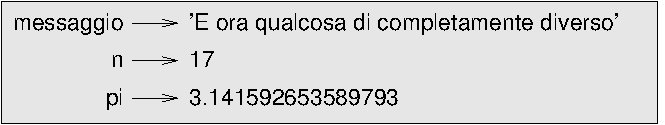
\includegraphics[scale=0.8]{figs/state2.pdf}}
\caption{Diagramma di stato.}
\label{fig.state2}
\end{figure}

\section{Nomi delle variabili}
\index{variabile}

Generalmente, i programmatori chiamano le variabili con dei nomi significativi, in modo da documentare a cosa servono.

I nomi possono essere lunghi a piacere e possono contenere sia lettere che numeri, ma non possono iniziare con un numero. È possibile usare anche le lettere maiuscole, ma per i nomi di variabile è convenzione utilizzare solo lettere minuscole. In ogni caso, tenete conto che, per l'interprete, maiuscole e minuscole sono diverse, pertanto \verb"spam", \verb"Spam" e \verb"SPAM" sono variabili diverse.

Il trattino basso o {\em underscore}, \verb"_", può far parte di un nome: è usato spesso in nomi di variabile composti da più parole (per esempio 
\verb"il_tuo_nome" o \verb"monty_python").
\index{underscore, carattere}

Se assegnate un nome non valido alla variabile, otterrete un errore di sintassi:

\begin{verbatim}
>>> 76tromboni = 'grande banda'
SyntaxError: invalid syntax
>>> altro@ = 1000000
SyntaxError: invalid syntax
>>> class = 'Zymurgy Teorico Avanzato'
SyntaxError: invalid syntax
\end{verbatim}
%
{\tt 76tromboni} non è valido perché non inizia con una lettera.
{\tt altro@} non è valido perché contiene un carattere non ammesso (la chiocciola {\tt @}). Ma cosa c'è di sbagliato in {\tt class}?

Succede che {\tt class} è una delle {\bf parole chiave riservate} di Python. L'interprete utilizza queste parole per riconoscere la struttura del programma, pertanto non è consentito usarle come nomi di variabile.
\index{parola chiave}

Python 3 ha queste parole chiave:

\begin{verbatim}
False      class      finally    is         return
None       continue   for        lambda     try
True       def        from       nonlocal   while
and        del        global     not        with
as         elif       if         or         yield
assert     else       import     pass
break      except     in         raise
\end{verbatim}
%
Non occorre imparare a memoria questo elenco. Nella maggior parte degli ambienti di sviluppo, le parole chiave vengono evidenziate con un diverso colore; se cercate di usarne una come nome di variabile, ve ne accorgerete subito.


\section{Espressioni e istruzioni}

Un'{\bf espressione} è una combinazione di valori, variabili e operatori. Un valore è considerato già di per sé un'espressione, come pure una variabile, per cui quelle che seguono sono tutte delle espressioni valide (supponendo che alla variabile {\tt n} sia già stato assegnato un valore):
\index{espressione}
\index{valutazione}

\begin{verbatim}
>>> 42
42
>>> n
17
>>> n + 25
42
\end{verbatim}
%

Quando scrivete un'espressione al prompt dei comandi, l'interprete la
{\bf valuta}, cioè trova il valore dell'espressione. 
Nell'esempio di prima, {\tt n} ha valore 17 e {\tt n + 25} ha valore 42.
\index{valutazione}

Un'{\bf istruzione} è una porzione di codice che l'interprete Python può eseguire e che ha un qualche effetto, come creare una variabile o mostrare un valore.

\begin{verbatim}
>>> n = 17
>>> print(n)
\end{verbatim}
%
La prima riga è un'istruzione di assegnazione che dà un valore alla variabile {\tt n}.  La seconda è un'istruzione di stampa che mostra a video il valore di {\tt n}.

Quando scrivete un'istruzione, l'interprete la {\bf esegue}, cioè fa quello che l'istruzione dice di fare. In linea generale, le istruzioni, a differenza delle espressioni, non contengono valori.
\index{esecuzione}


\section{Modalità script}

Finora abbiamo avviato Python in {\bf modalità interattiva}, detta anche ``a riga di comando'', che vuol dire interagire direttamente con l'interprete. La modalità interattiva è un buon modo per iniziare e fare esperimenti, ma se si deve lavorare con più di qualche riga di codice, può diventare in breve tempo un impiccio.

In alternativa alla riga di comando, si può scrivere e salvare un programma in un file di testo semplice, chiamato {\bf script}, ed usare poi l'interprete in {\bf modalità script} per eseguirlo. Per convenzione, i file contenenti programmi Python hanno nomi che terminano con l'estensione {\tt .py} .
\index{script}
\index{modalità script}

Se già sapete come creare e avviare uno script nel vostro computer, siete a cavallo. Altrimenti vi consiglio di nuovo di usare PythonAnywhere. Le istruzioni per l'avvio in modalità script sono pubblicate all'indirizzo
\url{http://tinyurl.com/thinkpython2e}.

Poiché Python consente entrambe queste modalità, potete provare dei pezzi di codice in modalità interattiva prima di inserirli in uno script. Ma tra le due modalità, ci sono delle differenze che possono disorientare.
\index{modalità interattiva}
\index{modalità script}

Per esempio, usando Python come una calcolatrice, si può scrivere:

\begin{verbatim}
>>> miglia = 26.2
>>> miglia * 1.61
42.182
\end{verbatim}

La prima riga assegna un valore a {\tt miglia}, e non ha alcun effetto visibile. La seconda riga è un'espressione, e l'interprete la valuta e ne mostra il risultato. Vediamo così che una maratona misura circa 42 chilometri.

Ma se scrivete lo stesso codice in uno script e lo avviate, non otterrete alcun riscontro. In modalità script, un'espressione, di per sé, non ha effetti visibili. In realtà Python valuta l'espressione, ma non ne mostra il risultato finché non gli dite esplicitamente di farlo:

\begin{verbatim}
miglia = 26.2
print(miglia * 1.61)
\end{verbatim}

Questo comportamento inizialmente può confondere.

Uno script di solito contiene una serie di istruzioni. Se ci sono più istruzioni, i risultati compaiono uno alla volta, man mano che le istruzioni vengono eseguite.

Per esempio lo script:

\begin{verbatim}
print(1)
x = 2
print(x)
\end{verbatim}
%
visualizza questo:

\begin{verbatim}
1
2
\end{verbatim}
%
mentre l'istruzione di assegnazione non produce alcun output sullo schermo.

Per controllare se avete capito tutto, scrivete le seguenti istruzioni nell'interprete Python per vedere quali effetti producono:

\begin{verbatim}
5
x = 5
x + 1
\end{verbatim}
%
Ora scrivete le stesse istruzioni in uno script ed avviatelo. Qual è il risultato? Modificate lo script trasformando ciascuna espressione in un'istruzione di stampa, ed avviatelo nuovamente.


\section{Ordine delle operazioni}
\index{ordine delle operazioni}
\index{PEMDAS}

Quando un'espressione contiene più operatori, la successione con cui viene eseguito il calcolo dipende dall'{\bf ordine delle operazioni}. Per quelle matematiche, Python segue le stesse regole di precedenza comunemente usate in matematica. L'acronimo {\bf PEMDAS} è un modo utile per ricordare le regole:

\begin{itemize}

\item {\bf P}arentesi: hanno il livello di precedenza più elevato e possono essere usate per forzare la valutazione di un'espressione secondo qualsiasi ordine si desideri. Dato che le espressioni tra parentesi sono valutate per prime, {\tt 2 * (3-1)} fa 4, e {\tt (1+1)**(5-2)} fa 8. Si possono usare le parentesi anche solo per rendere più leggibile un'espressione, come in {\tt (minuti * 100) / 60}, e in questo caso non influiscono sul risultato.

\item {\bf E}levamento a potenza: ha la priorità successiva, così
{\tt 1 + 2**3} fa 9, e non 27, e {\tt 2 * 3**2} fa 18, e non 36.

\item {\bf M}oltiplicazione e {\bf D}ivisione hanno priorità superiore ad {\bf A}ddizione e {\bf S}ottrazione. Per cui {\tt 2*3-1} fa 5, e non 4, e {\tt 6+4/2} fa 8, e non 5.

\item Gli operatori con la stessa priorità vengono valutati da sinistra verso destra (eccetto la potenza), per cui nell'espressione {\tt gradi / 2 * pi}, la divisione viene calcolata per prima e il risultato viene moltiplicato per {\tt pi}.  Per dividere {\tt gradi} per $2 \pi$, dovete usare le parentesi o scrivere {\tt gradi / 2 / pi}.

\end{itemize}

Personalmente, non mi sforzo molto di ricordare la precedenza degli operatori. Se non ne sono certo guardando un'espressione, inserisco le parentesi per fugare ogni dubbio.

\section{Operazioni sulle stringhe}
\index{stringa!operazioni}
\index{operatore!stringa}

In linea generale non è possibile effettuare operazioni matematiche sulle stringhe, anche se la stringa sembra un numero; quindi gli esempi che seguono non sono validi.

\begin{verbatim}
'2'-'1'    'uova'/'facili'    'terzo'*'una magia'
\end{verbatim}
%
Ma ci sono due eccezioni: {\tt +} e {\tt *}.

L'operatore {\tt +} esegue il {\bf concatenamento}, cioè unisce le stringhe collegandole ai due estremi. Per esempio:
\index{concatenamento}

\begin{verbatim}
>>> primo = 'bagno'
>>> secondo = 'schiuma'
>>> primo + secondo
bagnoschiuma
\end{verbatim}
%

Anche l'operatore {\tt *} funziona sulle stringhe: ne esegue la ripetizione. Per esempio, \verb"'Spam'*3" dà \verb"'SpamSpamSpam'". Uno degli operandi deve essere una stringa, l'altro un numero intero.

Questo utilizzo di {\tt +} e {\tt *} è coerente per analogia con l'addizione e la moltiplicazione. Dato che {\tt 4*3} è equivalente a {\tt 4+4+4}, ci possiamo aspettare che \verb"'Spam'*3" sia la stessa cosa di
\verb"'Spam'+'Spam'+'Spam'", ed infatti è così. Tuttavia, concatenamento e ripetizione di stringhe differiscono da addizione e moltiplicazione di interi per un particolare importante. Riuscite a pensare ad una proprietà che ha l'addizione ma che non vale per il concatenamento di stringhe?
\index{commutatività}


\section{Commenti}
\index{commento}

Al crescere delle sue dimensioni e della sua complessità, un programma diventa anche sempre più difficile da leggere. I linguaggi formali sono densi di significato, e spesso non è facile guardare un segmento di codice scritto da altri e capire immediatamente che cosa fa, o perché.

Per questo motivo, è buona abitudine aggiungere ai vostri programmi delle annotazioni che spiegano in linguaggio naturale ciò che il programma sta facendo. Queste annotazioni si chiamano {\bf commenti}, contrassegnati dal simbolo \verb"#":

\begin{verbatim}
# calcola la percentuale di ora trascorsa
percentuale = (minuti * 100) / 60
\end{verbatim}
%
In questo caso, il commento si trova su una riga a sé stante, ma potete anche inserire un commento in coda a una riga:

\begin{verbatim}
percentuale = (minuti * 100) / 60     # percentuale di un'ora
\end{verbatim}
%
Tutto ciò che viene scritto dopo il simbolo {\tt \#} e fino alla fine della riga, viene trascurato e non influisce in alcun modo sull'esecuzione del programma. 

I commenti più utili sono quelli che documentano caratteristiche del codice di non immediata comprensione. È ragionevole supporre che chi legge il codice possa capire {\em cosa} esso faccia; è più utile spiegare {\em perché}.

Questo commento è ridondante e inutile:

\begin{verbatim}
v = 5     # assegna 5 a v
\end{verbatim}
%
Questo commento contiene invece un'informazione utile che non è contenuta nel codice:

\begin{verbatim}
v = 5     # velocità in metri/secondo 
\end{verbatim}
%
Dei buoni nomi di variabile possono ridurre la necessità di commenti, ma nomi lunghi possono complicare la lettura, pertanto va trovato un giusto compromesso.


\section{Debug}
\index{debug}

In un programma si possono verificare tre tipi di errori: gli errori di sintassi, gli errori in esecuzione e gli errori di semantica. È utile analizzarli singolarmente per facilitarne l'individuazione.

\subsection{Errori di sintassi}
\index{sintassi!errore di}
\index{errore!di sintassi}
\index{errore!messaggio di}

Il termine {\bf sintassi} si riferisce alla struttura di un programma e alle regole che la governano. Ad esempio, le parentesi devono essere sempre presenti a coppie corrispondenti, così {\tt (1 + 2)} è corretto, ma {\tt 8)} è un {\bf errore di sintassi}.
\index{sintassi} 
\index{parentesi!corrispondenza}

Se c'è anche un solo errore di sintassi in qualche parte del programma, non sarete in grado di eseguirlo: Python visualizzerà subito un messaggio d'errore e lo terminerà. Nelle prime settimane della vostra carriera di programmatori, dovrete probabilmente dedicare molto tempo a correggere errori di sintassi. Ma con l'esperienza, ne commetterete meno e li troverete più velocemente.

\subsection{Errori in esecuzione}
\label{runtime}

Il secondo tipo di errore è l'{\bf errore in esecuzione} (o di {\em runtime}), così chiamato perché non compare fino a quando il programma non viene eseguito. Questi errori sono anche detti {\bf eccezioni} perché indicano che è accaduto qualcosa di eccezionale (e di spiacevole) durante l'esecuzione.
\index{errore!in esecuzione}
\index{errore!di runtime}
\index{eccezione}
\index{linguaggio!sicuro}

Gli errori di runtime sono molto rari nei programmi semplici, come quelli che vedrete nei primi capitoli di questo libro, e potrebbe passare un po' di tempo prima di incontrarne uno.


\subsection{Errori di semantica}
\index{semantica}
\index{semantica!errore di}
\index{errore!di semantica}
\index{errore!messaggio di}

Il terzo tipo di errore è l'{\bf errore di semantica} (o di logica), che è correlato al significato del programma. In presenza di un errore di semantica, il programma verrà eseguito senza che compaia alcun messaggio di errore, ma non farà la cosa giusta: farà qualcosa di diverso. Nello specifico, farà esattamente ciò che voi gli avete detto di fare, esprimendovi in modo sbagliato.

Gli errori di semantica sono insidiosi e identificarli può essere complicato, perché occorre lavorare a ritroso, partendo dai risultati dell'esecuzione e cercando di risalire a che cosa non sia andato per il verso giusto.


\section{Glossario}

\begin{description}

\item[variabile:]  Un nome che fa riferimento ad un valore.
\index{variabile}

\item[assegnazione:]  Istruzione che assegna un valore ad una variabile.
\index{assegnazione}

\item[diagramma di stato:]  Rappresentazione grafica di una serie di variabili e dei valori ai quali esse si riferiscono.
\index{diagramma!di stato}

\item[parola chiave riservata:]  Parola chiave destinata esclusivamente all'analisi del programma e che non può essere usata come nome di variabile o di funzione, come {\tt if}, {\tt  def}, e {\tt while}.
\index{parola chiave}

\item[operando:]  Uno dei valori sui quali si applica un operatore.
\index{operando}

\item[espressione:]  Combinazione di variabili, operatori e valori che rappresentano un unico valore risultante.
\index{espressione}

\item[valutare:]  Semplificare un'espressione eseguendo una serie di operazioni che producono un unico valore.
\index{valutazione}

\item[istruzione:]  Porzione di codice che rappresenta un comando o un'azione, come le istruzioni di assegnazione e di stampa che abbiamo visto finora.
\index{istruzione}

\item[eseguire:]  Dare efficacia a un'istruzione e fare ciò che dice.
\index{esecuzione}

\item[modalità interattiva:] Un modo di usare l'interprete Python, scrivendo del codice al prompt.
\index{modalità interattiva}

\item[modalità script:] Un modo di usare l'interprete Python, leggendo del codice da uno script ed eseguendolo.
\index{modalità script}

\item[script:] Un programma scritto e memorizzato in un file di testo.
\index{script}

\item[ordine delle operazioni:]  Regole che stabiliscono l'ordine in cui vengono valutate le espressioni che contengono più operandi ed operatori.
\index{ordine delle operazioni}

\item[concatenare:]  Unire due stringhe accodando la seconda alla prima.
\index{concatenamento}

\item[commento:]  Annotazione in un programma, rivolta ad altri programmatori (o a chi legge il codice sorgente), che non ha effetti sull'esecuzione del programma.
\index{commento}

\item[errore di sintassi:]  Errore in un programma che ne rende impossibile l'analisi (il programma non è interpretabile).
\index{sintassi!errore di}

\item[eccezione:]  Errore (detto anche di {\em runtime}) che si verifica mentre il programma è in esecuzione.
\index{eccezione}

\item[semantica:]  Il significato logico di un programma.
\index{semantica}

\item[errore di semantica:]   Errore nel programma tale da produrre risultati diversi da quelli che il programmatore si aspettava.
\index{semantica!errore di}

\end{description}


\section{Esercizi}

\begin{exercise}

Rinnovo la raccomandazione del capitolo precedente: ogni volta che apprendete qualcosa di nuovo, provatelo in modalità interattiva e fate degli errori di proposito per vedere cosa non funziona.

\begin{itemize}

\item Abbiamo visto che {\tt n = 42} è valido. E {\tt 42 = n}?

\item E se scrivete {\tt x = y = 1}?

\item In alcuni linguaggi, ogni istruzione termina con un punto e virgola, {\tt ;}.
Cosa succede se mettete un punto e virgola alla fine di un'istruzione in Python?

\item E se mettete un punto alla fine di un'istruzione?

\item Nella notazione matematica potete indicare la moltiplicazione di $x$ per $y$ scrivendo: $x y$. 
Cosa succede scrivendo questo in Python?

\end{itemize}

\end{exercise}

\vspace{0.2in}
\begin{exercise}

Fate un po' di pratica con l'interprete Python usandolo come calcolatrice:
\index{calcolatrice}

\begin{enumerate}

\item Il volume di una sfera di raggio $r$ è $\frac{4}{3} \pi r^3$.
  Che volume ha una sfera di raggio 5?

\item Il prezzo di copertina di un libro è \verb"€" 24,95, ma una libreria ottiene il 40\% di sconto. I costi di spedizione sono \verb"€" 3 per la prima copia e 75 centesimi per ogni copia aggiuntiva. Qual è il costo totale di 60 copie?

\item Se uscite di casa alle 6:52 di mattina e correte 1 miglio a ritmo blando (8:15 al miglio), poi 3 miglia a ritmo moderato (7:12 al miglio), quindi 1 altro miglio a ritmo blando, a che ora tornate a casa per colazione?
\index{cadenza di corsa}

\end{enumerate}
\end{exercise}


\chapter{Funzioni}
\label{funcchap}

Nell'ambito della programmazione, una {\bf funzione} è una serie di istruzioni che esegue un calcolo, alla quale viene assegnato un nome.  Per definire una funzione, dovete specificarne il nome e scrivere la serie di istruzioni. In un secondo tempo, potete ``chiamare'' la funzione mediante il nome che le avete assegnato. 
\index{funzione}

\section{Chiamate di funzione}
\label{functionchap}
\index{funzione!chiamata di}

Abbiamo già visto un esempio di una {\bf chiamata di funzione}:

\begin{verbatim}
>>> type(42)
<class 'int'>
\end{verbatim}
%
Il nome di questa funzione è {\tt type}. L'espressione tra parentesi è chiamata {\bf argomento} della funzione, e il risultato che produce è il tipo di valore dell'argomento che abbiamo inserito.
\index{parentesi!argomento in}

Si usa dire che una funzione ``prende'' o ``riceve'' un argomento e, una volta eseguita l'elaborazione, ``ritorna'' o ``restituisce'' un risultato.  Il risultato è detto {\bf valore di ritorno}.
\index{argomento}
\index{valore di ritorno}

Python contiene una raccolta di funzioni per convertire i valori da un tipo a un altro. La funzione {\tt int} prende un dato valore e lo converte, se possibile, in un numero intero. Se la conversione è impossibile, Python comunica che si è verificato un errore:
\index{conversione!di tipo}
\index{int, funzione}
\index{funzione!int}

\begin{verbatim}
>>> int('32')
32
>>> int('Ciao')
ValueError: invalid literal for int(): Ciao
\end{verbatim}
%
{\tt int} può anche convertire valori in virgola mobile in interi, ma non arrotonda bensì tronca la parte decimale.

\begin{verbatim}
>>> int(3.99999)
3
>>> int(-2.3)
-2
\end{verbatim}
%
La funzione {\tt float} converte interi e stringhe in numeri a virgola mobile:
\index{float, funzione}
\index{funzione!float}

\begin{verbatim}
>>> float(32)
32.0
>>> float('3.14159')
3.14159
\end{verbatim}
%
Infine, {\tt str} converte l'argomento in una stringa:
\index{str, funzione}
\index{funzione!str}

\begin{verbatim}
>>> str(32)
'32'
>>> str(3.14159)
'3.14159'
\end{verbatim}
%

\section{Funzioni matematiche}
\index{funzioni matematiche}

Python è provvisto di un modulo matematico che comprende buona parte delle funzioni matematiche d'uso frequente. Un {\bf modulo} è un file che contiene una raccolta di funzioni correlate.
\index{modulo}
\index{oggetto!modulo}

Prima di poter usare le funzioni contenute in un modulo, lo dobbiamo importare con un'{\bf istruzione di importazione}:

\begin{verbatim}
>>> import math
\end{verbatim}
%
Questa istruzione crea un {\bf oggetto modulo} chiamato math. Se visualizzate l'oggetto modulo, ottenete alcune informazioni a riguardo:

\begin{verbatim}
>>> math
<module 'math' (built-in)>
\end{verbatim}
%
L'oggetto modulo contiene le funzioni e le variabili definite all'interno del modulo stesso. Per accedere a una funzione del modulo, dovete specificare, nell'ordine, il nome del modulo e il nome della funzione, separati da un punto. Questo formato è chiamato {\bf notazione a punto} o {\em dot notation}.
\index{dot notation}
\index{notazione a punto}

\begin{verbatim}
>>> rapporto = potenza_segnale / potenza_rumore
>>> decibel = 10 * math.log10(rapporto)

>>> radianti = 0.7
>>> altezza = math.sin(radianti)
\end{verbatim}
%
Il primo esempio utilizza la funzione \verb"math.log10" per calcolare un rapporto segnale/rumore in decibel (a condizione che siano stati definiti i valori di \verb"potenza_segnale" e \verb"potenza_rumore").  Il modulo math contiene anche {\tt log}, che calcola i logaritmi naturali in base {\tt e}.
\index{log, funzione}
\index{funzione!log}
\index{seno, funzione}
\index{radiante}
\index{funzione!trigonometrica}


Il secondo esempio calcola il seno della variabile {\tt radianti}. Il nome della variabile spiega già che {\tt sin} e le altre funzioni trigonometriche ({\tt cos}, {\tt tan}, ecc.) accettano argomenti espressi in radianti. Per convertire da gradi in radianti occorre dividere per 180 e moltiplicare per $\pi$:

\begin{verbatim}
>>> gradi = 45
>>> radianti = gradi / 180.0 * math.pi
>>> math.sin(radianti)
0.707106781187
\end{verbatim}
%
L'espressione {\tt math.pi} ricava la variabile {\tt pi} dal modulo matematico. Il suo valore è un numero decimale, approssimazione di $\pi$, accurata a circa 15 cifre. 
\index{pi}

Se ricordate la trigonometria, potete verificare il risultato precedente confrontandolo con la radice quadrata di 2 diviso 2:
\index{sqrt, funzione}
\index{funzione!sqrt}

\begin{verbatim}
>>> math.sqrt(2) / 2.0
0.707106781187
\end{verbatim}
%

\section{Composizione}
\index{composizione}

Finora, abbiamo considerato gli elementi di un programma - variabili, espressioni e istruzioni - separatamente, senza discutere di come utilizzarli insieme.

Una delle caratteristiche più utili dei linguaggi di programmazione è la loro capacità di prendere dei piccoli mattoni e {\bf comporli} tra loro. Per esempio, l'argomento di una funzione può essere un qualunque tipo di espressione, operazioni aritmetiche incluse:

\begin{verbatim}
x = math.sin(gradi / 360.0 * 2 * math.pi)
\end{verbatim}
%
E anche chiamate di funzione:

\begin{verbatim}
x = math.exp(math.log(x+1))
\end{verbatim}
%
In linea generale, dovunque potete mettere un valore potete anche mettere un'espressione a piacere, con un'eccezione: il lato sinistro di un'istruzione di assegnazione deve essere un nome di variabile. Ogni altra espressione darebbe un errore di sintassi (vedremo più avanti le eccezioni a questa regola).

\begin{verbatim}
>>> minuti = ore * 60                 # giusto
>>> ore * 60 = minuti                 # sbagliato!
SyntaxError: can't assign to operator
\end{verbatim}
%
\index{SyntaxError}
\index{eccezione!SyntaxError}


\section{Aggiungere nuove funzioni}

Finora abbiamo usato solo funzioni predefinite o ``built-in'', che sono parte integrante di Python, ma è anche possibile crearne di nuove.
Una {\bf definizione di funzione} specifica il nome di una nuova funzione e la serie di istruzioni che viene eseguita quando la funzione viene chiamata.
\index{funzione}
\index{funzione!definizione di}
\index{definizione!di funzione}

Ecco un esempio:

\begin{verbatim}
def stampa_brani():
    print('Terror di tutta la foresta egli è,')
    print("Con l'ascia in mano si sente un re.")
\end{verbatim}
%
{\tt def} è una parola chiave riservata che indica la definizione di una nuova funzione. Il nome della funzione è \verb"stampa_brani".  Le regole per i nomi delle funzioni sono le stesse dei nomi delle variabili: lettere, numeri e underscore (\verb"_") sono permessi, ma il primo carattere non può essere un numero. Non si possono usare parole riservate, e bisogna evitare di avere una funzione e una variabile con lo stesso nome
\index{def, parola chiave}
\index{parola chiave!def}
\index{argomento}

Le parentesi vuote dopo il nome indicano che la funzione non accetta alcun argomento.
\index{parentesi!vuote}
\index{intestazione}
\index{corpo}
\index{indentazione}
\index{due punti}

La prima riga della definizione di funzione è chiamata {\bf intestazione};
il resto è detto {\bf corpo}. L'intestazione deve terminare con i due punti, e il corpo deve essere obbligatoriamente indentato, cioè deve avere un rientro rispetto all'intestazione. Per convenzione, l'indentazione è sempre di quattro spazi. Il corpo può contenere un qualsiasi numero di istruzioni.

Le stringhe nelle istruzioni di stampa sono racchiuse tra apici (\verb"' '") oppure virgolette (\verb'" "'). Virgolette e apici sono equivalenti; la maggioranza degli utenti usa gli apici, eccetto nei casi in cui nel testo da stampare sono contenuti degli apici (che possono essere usati anche come apostrofi o accenti). In questi casi, frequenti con l'italiano, bisogna usare le virgolette.

Virgolette e apici devono essere alti e di tipo indifferenziato, quelli che trovate tra i simboli in alto sulla vostra tastiera.  Altre virgolette ``tipografiche'', come quelle in questa frase, non sono valide in Python.

Se scrivete una funzione in modalità interattiva, l'interprete mette tre puntini di sospensione ({\em ...}) per indicare che la definizione non è completa:
\index{ellissi}

\begin{verbatim}
>>> def stampa_brani():
...     print('Terror di tutta la foresta egli è,')
...     print("Con l'ascia in mano si sente un re.")
...
\end{verbatim}
%
Per concludere la funzione, dovete inserire una riga vuota.

La definizione di una funzione crea un {\bf oggetto funzione} che è di tipo \verb"function":
\index{tipo!function}
\index{oggetto!funzione}

\begin{verbatim}
>>> print(stampa_brani)
<function stampa_brani at 0xb7e99e9c>
>>> type(stampa_brani)
<class 'function'>
\end{verbatim}
%

La sintassi per chiamare la nuova funzione è la stessa che abbiamo visto per le funzioni predefinite:

\begin{verbatim}
>>> stampa_brani()
Terror di tutta la foresta egli è,
Con l'ascia in mano si sente un re.
\end{verbatim}
%
Una volta definita una funzione, si può utilizzarla all'interno di un'altra funzione. Per esempio, per ripetere due volte il brano precedente possiamo scrivere una funzione \verb"ripeti_brani":

\begin{verbatim}
def ripeti_brani():
    stampa_brani()
    stampa_brani()
\end{verbatim}
%
E quindi chiamare \verb"ripeti_brani":

\begin{verbatim}
>>> ripeti_brani()
Terror di tutta la foresta egli è,
Con l'ascia in mano si sente un re.
Terror di tutta la foresta egli è,
Con l'ascia in mano si sente un re.
\end{verbatim}
%
Ma a dire il vero, la canzone del taglialegna non fa così!


\section{Definizioni e loro utilizzo}
\index{funzione!definizione di}

Raggruppando assieme i frammenti di codice del Paragrafo precedente, il programma diventa:

\begin{verbatim}
def stampa_brani():
    print('Terror di tutta la foresta egli è,')
    print("Con l'ascia in mano si sente un re.")

def ripeti_brani():
    stampa_brani()
    stampa_brani()

ripeti_brani()
\end{verbatim}
%

Questo programma contiene due definizioni di funzione: \verb"stampa_brani" e
\verb"ripeti_brani".  Le definizioni di funzione sono eseguite come le altre istruzioni, ma il loro effetto è solo quello di creare una nuova funzione. Le istruzioni all'interno di una definizione non vengono eseguite fino a quando la funzione non viene chiamata, e la definizione di per sé non genera alcun risultato.

Ovviamente, una funzione deve essere definita prima di poterla usare: la definizione della funzione deve sempre precedere la sua chiamata.
\index{uso prima di def}

Come esercizio, spostate l'ultima riga del programma all'inizio, per fare in modo che la chiamata della funzione appaia prima della definizione. Eseguite il programma e guardate che tipo di messaggio d'errore ottenete.

Ora riportate la chiamata della funzione al suo posto, e spostate la definizione di \verb"stampa_brani" dopo la definizione di \verb"ripeti_brani". Cosa succede quando avviate il programma?


\section{Flusso di esecuzione}
\index{flusso di esecuzione}

Per essere sicuri che una funzione sia stata definita prima di essere utilizzata, dovete conoscere l'ordine in cui le istruzioni vengono eseguite, che è chiamato {\bf flusso di esecuzione}.

L'esecuzione inizia sempre dalla prima istruzione del programma; quindi, le istruzioni successive sono eseguite una alla volta, procedendo dall'alto verso il basso.

Le definizioni di funzione non cambiano il flusso di esecuzione del programma, ma ricordate che le istruzioni all'interno delle funzioni non vengono eseguite fino a quando la funzione non viene chiamata. 

Quando viene chiamata una funzione, si genera una specie di deviazione nel flusso di esecuzione: anziché proseguire con l'istruzione successiva, il flusso salta nel corpo della funzione chiamata, ne esegue le istruzioni, e infine riprende il percorso dal punto che aveva lasciato.

Parrebbe tutto abbastanza semplice, se non fosse che una funzione può chiamarne un'altra. Mentre si trova all'interno di una funzione, il programma può dover eseguire le istruzioni che si trovano in un'altra funzione. Poi, mentre esegue quella nuova funzione, il programma potrebbe andare ad eseguirne un'altra ancora!

Fortunatamente, Python sa tener bene traccia di dove si trova: ogni volta che una funzione viene completata, il programma ritorna al punto della funzione chiamante che aveva lasciato. E una volta giunto alla fine, termina il suo lavoro.

Concludendo, nel leggere un programma non è sempre opportuno farlo dall'alto in basso. Spesso è più logico seguire il flusso di esecuzione.


\section{Parametri e argomenti}
\label{parametri}
\index{parametro}
\index{funzione!parametro di}
\index{argomento}
\index{funzione!argomento di}

Alcune delle funzioni che abbiamo visto richiedono degli argomenti. Per esempio, se volete trovare il seno di un numero chiamando la funzione {\tt math.sin}, dovete passarle quel numero come argomento. Alcune funzioni ricevono più di un argomento: a {\tt math.pow} ne servono due, che sono la base e l'esponente dell'operazione di elevamento a potenza. 

All'interno della funzione, gli argomenti che le vengono passati sono assegnati ad altrettante variabili chiamate {\bf parametri}. Ecco un esempio di definizione di una funzione che riceve un argomento:
\index{parentesi!parametri in}

\begin{verbatim}
def stampa2volte(bruce):
    print(bruce)
    print(bruce)
\end{verbatim}
%
Questa funzione assegna l'argomento ricevuto ad un parametro chiamato {\tt bruce}. Quando la funzione viene chiamata, stampa il valore del parametro (qualunque esso sia) due volte.

Questa funzione elabora qualunque valore che possa essere stampato.

\begin{verbatim}
>>> stampa2volte('Spam')
Spam
Spam
>>> stampa2volte(42)
42
42
>>> stampa2volte(math.pi)
3.14159265359
3.14159265359
\end{verbatim}
%
Le stesse regole di composizione che valgono per le funzioni predefinite si applicano anche alle funzioni definite da un programmatore, pertanto possiamo usare come argomento per \verb"stampa2volte" qualsiasi espressione:
\index{composizione}
\index{funzione!personalizzata}

\begin{verbatim}
>>> stampa2volte('Spam '*4)
Spam Spam Spam Spam
Spam Spam Spam Spam
>>> stampa2volte(math.cos(math.pi))
-1.0
-1.0
\end{verbatim}
%
L'argomento viene valutato prima della chiamata alla funzione, pertanto nell'esempio appena proposto le espressioni \verb"'Spam '*4" e
{\tt math.cos(math.pi)} vengono valutate una volta sola.
\index{argomento}

Potete anche usare una variabile come argomento di una funzione:

\begin{verbatim}
>>> michael = 'Eric, the half a bee.'
>>> stampa2volte(michael)
Eric, the half a bee.
Eric, the half a bee.
\end{verbatim}
%
Il nome della variabile che passiamo come argomento ({\tt michael}) non ha niente a che fare con il nome del parametro nella definizione della funzione ({\tt bruce}).  Non ha importanza come era stato denominato il valore di partenza (nel codice chiamante); qui in \verb"stampa2volte", chiamiamo tutto quanto {\tt bruce}.


\section{Variabili e parametri sono locali}
\index{variabile!locale}

Quando create una variabile in una funzione, essa è {\bf locale},
cioè esiste solo all'interno della funzione. Per esempio:
\index{parentesi!parametri in}

\begin{verbatim}
def cat2volte(parte1, parte2):
    cat = parte1 + parte2
    stampa2volte(cat)
\end{verbatim}
%
Questa funzione prende due argomenti, li concatena e poi stampa il risultato per due volte. Ecco un esempio che la utilizza:
\index{concatenamento}

\begin{verbatim}
>>> riga1 = 'Bing tiddle '
>>> riga2 = 'tiddle bang.'
>>> cat2volte(riga1, riga2)
Bing tiddle tiddle bang.
Bing tiddle tiddle bang.
\end{verbatim}
%
Quando \verb"cat2volte" termina, la variabile {\tt cat} viene distrutta. Se provassimo a stamparla, otterremmo infatti un messaggio d'errore:
\index{NameError}
\index{eccezione!NameError}

\begin{verbatim}
>>> print(cat)
NameError: name 'cat' is not defined
\end{verbatim}
%
Anche i parametri sono locali: esternamente alla funzione \verb"stampa2volte", non esiste nulla di nome {\tt bruce}.
\index{parametri}


\section{Diagrammi di stack}
\label{stackdiagram}
\index{diagramma!di stack}
\index{funzione!frame di}
\index{frame}

Per tenere traccia di quali variabili possono essere usate e dove, a volte può risultare utile disegnare un {\bf diagramma di stack}. Come i diagrammi di stato, i diagrammi di stack mostrano il valore di ciascuna variabile, ma in più indicano a quale funzione essa appartiene.

Ciascuna funzione è rappresentata da un {\bf frame}, un riquadro che riporta a fianco il nome della funzione e all'interno un elenco dei suoi parametri e delle sue variabili. Nel caso dell'esempio precedente, il diagramma di stack è illustrato in Figura~\ref{fig.stack}.

\begin{figure}
\centerline
{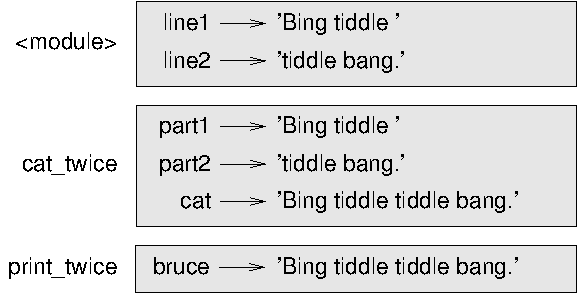
\includegraphics[scale=0.8]{figs/stack.pdf}}
\caption{Diagramma di stack.}
\label{fig.stack}
\end{figure}


I frame sono disposti in una pila che indica quale funzione ne ha chiamata un'altra e così via. Nell'esempio, \verb"stampa2volte" è stata chiamata da \verb"cat2volte", e \verb"cat2volte" è stata a sua volta chiamata da 
\verb"__main__", che è un nome speciale per il frame principale. Quando si crea una variabile che è esterna ad ogni funzione, essa appartiene a 
\verb"__main__".
\index{main}

Ogni parametro fa riferimento allo stesso valore del suo argomento corrispondente. Così, {\tt parte1} ha lo stesso valore di
{\tt riga1}, {\tt parte2} ha lo stesso valore di {\tt riga2},
e {\tt bruce} ha lo stesso valore di {\tt cat}.

Se si verifica un errore durante la chiamata di una funzione, Python mostra il nome della funzione, il nome della funzione che l'ha chiamata, il nome della funzione che a sua volta ha chiamato quest'ultima e così via, fino a raggiungere il primo livello che è sempre \verb"__main__".

Ad esempio se cercate di accedere a {\tt cat} dall'interno di
\verb"stampa2volte", ottenete un errore di tipo {\tt NameError}:

\begin{verbatim}
Traceback (innermost last):
  File "test.py", line 13, in __main__
    cat2volte(riga1, riga2)
  File "test.py", line 5, in cat2volte
    stampa2volte(cat)
  File "test.py", line 9, in stampa2volte
    print(cat)
NameError: name 'cat' is not defined
\end{verbatim}
%
Questo elenco di funzioni è detto {\bf traceback}. Il traceback vi dice in quale file è avvenuto l'errore, e in quale riga, e quale funzione era in esecuzione in quel momento. Mostra anche la riga di codice che ha causato l'errore.
\index{traceback}

L'ordine delle funzioni nel traceback è lo stesso di quello dei frame nel diagramma di stack. La funzione attualmente in esecuzione si trova in fondo all'elenco.


\section{Funzioni ``produttive'' e funzioni ``vuote''}
\index{funzione!produttiva}
\index{funzione!vuota} 

Alcune delle funzioni che abbiamo usato, come le funzioni matematiche, restituiscono dei risultati; in mancanza di definizioni migliori, personalmente le chiamo {\bf funzioni ``produttive''}.  Altre funzioni, come \verb"stampa2volte", eseguono un'azione ma non restituiscono alcun valore. Le chiameremo {\bf funzioni ``vuote''}.

Quando chiamate una funzione produttiva, quasi sempre è per fare qualcosa di utile con il suo risultato, tipo assegnarlo a una variabile o usarlo come parte di un'espressione.

\begin{verbatim}
x = math.cos(radianti)
aureo = (math.sqrt(5) + 1) / 2
\end{verbatim}
%
Se chiamate una funzione in modalità interattiva, Python ne mostra il risultato:

\begin{verbatim}
>>> math.sqrt(5)
2.2360679774997898
\end{verbatim}
%
Ma in uno script, se chiamate una funzione produttiva così come è, il valore di ritorno è perso!

\begin{verbatim}
math.sqrt(5)
\end{verbatim}
%
Questo script in effetti calcola la radice quadrata di 5, ma non conserva nè visualizza il risultato, per cui non è di grande utilità.
\index{modalità interattiva}
\index{modalità script}

Le funzioni vuote possono visualizzare qualcosa sullo schermo o avere qualche altro effetto, ma non restituiscono un valore. Se provate comunque ad assegnare il risultato ad una variabile, ottenete un valore speciale chiamato
{\tt None} (nulla).
\index{None, valore speciale}
\index{valore speciale!None}

\begin{verbatim}
>>> risultato = stampa2volte('Bing')
Bing
Bing
>>> print(risultato)
None
\end{verbatim}
%
Il valore {\tt None} non è la stessa cosa della stringa \verb"'None'". 
È un valore speciale che appartiene ad un tipo tutto suo:

\begin{verbatim}
>>> type(None)
<class 'NoneType'>
\end{verbatim}
%
Le funzioni che abbiamo scritto finora, sono tutte vuote. Cominceremo a scriverne di produttive tra alcuni capitoli.


\section{Perché usare le funzioni?}
\index{funzione!motivi}

Potrebbe non esservi ancora ben chiaro perché valga la pena di suddividere il programma in funzioni. Ecco alcuni motivi:

\begin{itemize}

\item Creare una nuova funzione vi dà modo di dare un nome a un gruppo di istruzioni, rendendo il programma più facile da leggere e da correggere.

\item Le funzioni possono rendere un programma più breve, eliminando il codice ripetitivo. Se in un secondo tempo dovete fare una modifica, basterà farla in un posto solo.

\item Dividere un programma lungo in funzioni vi permette di correggere le parti una per una, per poi assemblarle in un complesso funzionante.

\item Funzioni ben fatte sono spesso utili per più programmi. Quando ne avete scritta e corretta una, la potete riutilizzare tale e quale.

\end{itemize}


\section{Debug}
\label{editor}
\index{debug}

Saper rintracciare e correggere gli errori è una essenziale qualità che dovete acquisire. Anche se a volte può essere demotivante, si tratta infatti di una delle parti più intellettualmente ricche, stimolanti ed interessanti della programmazione.
\index{debug!sperimentale}

Possiamo paragonare il debug al lavoro di un investigatore: avete a disposizione degli indizi e dovete ricostruire quali processi ed eventi hanno prodotto il risultato che osservate.

Il debug è anche simile ad una scienza sperimentale. Quando pensate di aver capito cosa può avere provocato un errore, modificate il programma di conseguenza e riprovate di nuovo. Se l'ipotesi era giusta, avete saputo prevedere il risultato della modifica e vi siete avvicinati di un passo ad un programma funzionante. Se l'ipotesi era sbagliata, ne dovete formulare un'altra. Come disse Sherlock Holmes: ``Una volta eliminato l'impossibile, qualsiasi cosa rimanga, per quanto improbabile, deve essere la verità.''
(A. Conan Doyle, {\em Il segno dei quattro})
\index{Holmes, Sherlock}
\index{Doyle, Arthur Conan}

Per alcuni, la programmazione e la rimozione degli errori sono in fondo la stessa cosa: programmare è una procedura di graduale rimozione degli errori da un programma, fino a quando non funziona a dovere. L'idea di fondo è di iniziare con un programma funzionante e di fare ogni volta piccole modifiche, effettuandone man mano il debug.

Linux, ad esempio, è un sistema operativo fatto da milioni di righe di codice, ma nacque come un semplice programma che Linus Torvalds usava per esplorare il chip Intel 80386. Secondo Larry Greenfields, ``Uno dei progetti iniziali di Linus era un programma che doveva visualizzare alternativamente una sequenza di AAAA e BBBB. Questo programma si è poi evoluto in Linux''. ({\em The Linux Users' Guide} Beta Version 1).
\index{Linux}

\section{Glossario}

\begin{description}

\item[funzione:] Una serie di istruzioni dotata di un nome che esegue una certa operazione utile. Le funzioni possono o meno ricevere argomenti e possono o meno produrre un risultato.
\index{funzione}

\item[definizione di funzione:]  Istruzione che crea una nuova funzione, specificandone il nome, i parametri, e le istruzioni che contiene.
\index{funzione!definizione di}

\item[oggetto funzione:]  Valore creato da una definizione di funzione. Il nome della funzione è una variabile che fa riferimento a un oggetto funzione.
\index{oggetto!funzione}

\item[intestazione:] La prima riga di una definizione di funzione.
\index{intestazione}

\item[corpo:] La serie di istruzioni all'interno di una definizione di funzione.
\index{corpo}

\item[parametro:] Un nome usato all'interno di una funzione che fa riferimento al valore passato come argomento.
\index{parametro}

\item[chiamata di funzione:] Istruzione che esegue una funzione. Consiste nel nome della funzione seguito da un elenco di argomenti tra parentesi.
\index{funzione!chiamata di}

\item[argomento:]  Un valore fornito (passato) a una funzione quando viene chiamata. Questo valore viene assegnato al corrispondente parametro nella funzione.
\index{argomento}

\item[variabile locale:]  Variabile definita all'interno di una funzione e che puo essere usata solo all'interno della funzione.
\index{variabile!locale}

\item[valore di ritorno:]  Il risultato di una funzione. Se una chiamata di funzione viene usata come espressione, il valore di ritorno è il valore dell'espressione.
\index{valore di ritorno}

\item[funzione ``produttiva'':] Una funzione che restituisce un valore.
\index{funzione!produttiva}

\item[funzione ``vuota'':] Una funzione che restituisce sempre {\tt None}.
\index{funzione!vuota}

\item[{\tt None}:]  Valore speciale restituito dalle funzioni vuote.
\index{None, valore speciale}
\index{valore speciale!None}

\item[modulo:] Un file che contiene una raccolta di funzioni correlate e altre definizioni.
\index{modulo}

\item[istruzione import:] Istruzione che legge un file modulo e crea un oggetto modulo utilizzabile.
\index{import, istruzione}
\index{istruzione!import}

\item[oggetto modulo:] Valore creato da un'istruzione {\tt import} che fornisce l'accesso ai valori definiti in un modulo.
\index{modulo}

\item[dot notation o notazione a punto:]  Sintassi per chiamare una funzione di un modulo diverso, specificando il nome del modulo seguito da un punto e dal nome della funzione.
\index{dot notation}
\index{notazione a punto}

\item[composizione:] Utilizzare un'espressione come parte di un'espressione più grande o un'istruzione come parte di un'istruzione più grande.
\index{composizione}

\item[flusso di esecuzione:]  L'ordine in cui vengono eseguite le istruzioni nel corso di un programma.
\index{flusso di esecuzione}

\item[diagramma di stack:]  Rappresentazione grafica di una serie di funzioni impilate, delle loro variabili e dei valori a cui fanno riferimento.
\index{diagramma!di stack}

\item[frame:]  Un riquadro in un diagramma di stack che rappresenta una chiamata di funzione. Contiene le variabili locali e i parametri della funzione.
\index{funzione!frame di}
\index{frame}

\item[traceback:]  Elenco delle funzioni in corso di esecuzione, visualizzato quando si verifica un errore.
\index{traceback}


\end{description}


\section{Esercizi}

\begin{exercise}
\index{len, funzione}
\index{funzione!len}

Scrivete una funzione chiamata \verb"giustif_destra" che richieda una stringa {\tt s} come parametro e stampi la stringa con tanti spazi iniziali da far sì che l'ultima lettera della stringa cada nella colonna 70 del display.

\begin{verbatim}
>>> giustif_destra('monty')
                                                                 monty
\end{verbatim}

Suggerimento: usate concatenamento delle stringhe e ripetizione.  Inoltre,
Python contiene una funzione predefinita chiamata {\tt len} che restituisce la lunghezza di una stringa, ad esempio il valore di \verb"len('monty')" è 5.

\end{exercise}

\vspace{0.2in}
\begin{exercise}
\index{oggetto!funzione}

Un oggetto funzione è un valore che potete assegnare a una variabile o passare come argomento. Ad esempio, \verb"fai2volte" è una funzione che accetta un oggetto funzione come argomento e la chiama per due volte.

\begin{verbatim}
def fai2volte(f):
    f()
    f()
\end{verbatim}

Ecco un esempio che usa \verb"fai2volte" per chiamare una funzione di nome \verb"stampa_spam" due volte.

\begin{verbatim}
def stampa_spam():
    print('spam')

fai2volte(stampa_spam)
\end{verbatim}

\begin{enumerate}

\item Scrivete questo esempio in uno script e provatelo.

\item Modificate \verb"fai2volte" in modo che accetti due argomenti, un oggetto funzione e un valore, e che chiami la funzione due volte passando il valore come argomento.

\item Copiate nel vostro script la definizione di \verb"stampa_2volte" che abbiamo visto nel corso di questo capitolo.

\item Usate la versione modificata di \verb"fai2volte" per chiamare
\verb"stampa_2volte" per due volte, passando \verb"'spam'" come argomento.

\item Definite una nuova funzione di nome \verb"fai_quattro" che richieda un oggetto funzione e un valore e chiami la funzione per 4 volte, passando il valore come argomento. Dovrebbero esserci solo due istruzioni nel corpo di questa funzione, non quattro.

\end{enumerate}

Soluzione: \url{http://thinkpython2.com/code/do_four.py}.

\end{exercise}


\vspace{0.2in}
\begin{exercise}

Nota: questo esercizio dovrebbe essere svolto con le sole istruzioni e caratteristiche del linguaggio imparate finora.

\begin{enumerate}

\item Scrivete una funzione che disegni una griglia come questa:
\index{griglia}

\begin{verbatim}
+ - - - - + - - - - +
|         |         |
|         |         |
|         |         |
|         |         |
+ - - - - + - - - - +
|         |         |
|         |         |
|         |         |
|         |         |
+ - - - - + - - - - +
\end{verbatim}
%
Suggerimento: per stampare più di un valore per riga, stampate una sequenza di valori separati da virgole:

\begin{verbatim}
print('+', '-')
\end{verbatim}
%
Di default, {\tt print} va a capo; si può però variare questo comportamento e restare sulla stessa riga, inserendo uno spazio, in questo modo:

\begin{verbatim}
print('+', end=' ')
print('-')
\end{verbatim}
%
L'output di queste istruzioni è \verb"'+ -'".

Una funzione {\tt print} priva di argomento, termina la riga e va a capo.

\item Scrivete una funzione che disegni una griglia simile, con quattro righe e quattro colonne.

\end{enumerate}

Soluzione: \url{http://thinkpython2.com/code/grid.py}.
Fonte: Esercizio tratto da Oualline, {\em Practical C Programming, Third Edition}, O'Reilly Media, 1997.

\end{exercise}





\chapter{Esercitazione: Progettazione dell'interfaccia}
\label{turtlechap}

Questo capitolo vi propone un'esercitazione che dimostra una procedura per progettare delle funzioni che collaborano tra loro.

Viene illustrato il modulo grafico {\tt turtle} che vi permette di creare immagini utilizzando {\em turtle graphics}.  Si tratta di un modulo già compreso nella maggior parte delle installazioni di Python; tuttavia, se usate PythonAnywhere, non sarete in grado di visualizzare gli esempi basati su turtle (almeno non nel momento in cui scrivo).

Se avete già installato Python sul vostro computer, gli esempi dovrebbero funzionare. Se non lo avete ancora installato, questo è il momento buono per farlo. Potete trovare delle istruzioni all'indirizzo \url{http://tinyurl.com/thinkpython2e}.

Il codice degli esempi di questo capitolo è scaricabile dal sito
\url{http://thinkpython2.com/code/polygon.py}


\section{Il modulo turtle}
\label{turtle}

Per controllare se il modulo {\tt turtle} è installato, aprite l'interprete Python e scrivete:

\begin{verbatim}
>>> import turtle
>>> bob = turtle.Turtle()
\end{verbatim}

Eseguendo questo codice, dovrebbe comparire una nuova finestra con un cursore a forma di freccetta che rappresenta un'ideale tartaruga. Ora chiudete pure la finestra.

Create un file di nome {\tt miopoligono.py} e scriveteci il seguente codice:

\begin{verbatim}
import turtle
bob = turtle.Turtle()
print(bob)
turtle.mainloop()
\end{verbatim}
%
Il modulo {\tt turtle} (con la 't' minuscola) contiene una funzione di nome {\tt Turtle} (con la 'T' maiuscola) che crea un oggetto Turtle (una ``tartaruga''); questo oggetto viene assegnato a una variabile di nome {\tt bob}.
Stampando {\tt bob} viene visualizzato qualcosa di questo genere:

\begin{verbatim}
<turtle.Turtle object at 0xb7bfbf4c>
\end{verbatim}
%
Ciò significa che {\tt bob} fa riferimento ad un oggetto {\tt Turtle},
come definito nel modulo {\tt turtle}.

\verb"mainloop" dice alla finestra di attendere che l'utente faccia qualcosa, sebbene in questo caso non ci sia molto da fare, se non chiudere la finestra.

Una volta creata una tartaruga, potete chiamare uno dei suoi {\bf metodi} per spostarla in giro per la finestra.  Un metodo è simile ad una funzione, ma usa una sintassi leggermente diversa. Ad esempio, per spostare la tartaruga in avanti:

\begin{verbatim}
bob.fd(100)
\end{verbatim}
%
Il metodo, {\tt fd}, è associato all'oggetto Turtle che abbiamo chiamato
{\tt bob}.  
Chiamare un metodo è come effettuare una richiesta: in questo caso state chiedendo a {\tt bob} di muoversi in avanti [fd sta per {\em forward}, NdT].
L'argomento di {\tt fd} è una distanza espressa in pixel, per cui l'effettivo spostamento dipenderà dalle caratteristiche del vostro schermo.

Altri metodi che potete chiamare su una tartaruga sono: {\tt bk} per muoversi indietro ({\em backward}) e {\tt lt} e {\tt rt} per girare a sinistra ({\em left}) e a destra ({\em right}). Per questi ultimi due, l'argomento è un angolo espresso in gradi. 

Inoltre, ogni tartaruga regge una penna, che può essere appoggiata o sollevata; se la penna è appoggiata, la tartaruga lascia un segno dove passa. I metodi {\tt pu} e {\tt pd} stanno per ``penna su ({\em up})'' e ``penna giù ({\em down})''.

Per disegnare un angolo retto, aggiungete queste righe al programma (dopo aver creato {\tt bob} e prima di chiamare \verb"mainloop"):

\begin{verbatim}
bob.fd(100)
bob.lt(90)
bob.fd(100)
\end{verbatim}
%
Avviando il programma, dovreste vedere {\tt bob} muoversi verso destra e poi in alto, lasciandosi dietro due segmenti.

Ora provate a modificare il programma in modo da disegnare un quadrato. Non andate avanti finché non ci riuscite!

%\newpage

\section{Ripetizione semplice}
\label{repetition}
\index{ripetizione}

Probabilmente avete scritto qualcosa del genere:

\begin{verbatim}
bob.fd(100)
bob.lt(90)

bob.fd(100)
bob.lt(90)

bob.fd(100)
bob.lt(90)

bob.fd(100)
\end{verbatim}
%
Si può ottenere lo stesso risultato in modo più conciso con un'istruzione {\tt for}. Aggiungete questo esempio a {\tt miopoligono.py} ed eseguitelo di nuovo:
\index{for, ciclo}
\index{ciclo!for}
\index{istruzione!for}

\begin{verbatim}
for i in range(4):
    print('Ciao!')
\end{verbatim}
%
Dovreste vedere qualcosa di simile:

\begin{verbatim}
Ciao!
Ciao!
Ciao!
Ciao!
\end{verbatim}
%
Questo è l'utilizzo più semplice dell'istruzione {\tt for}; ne vedremo altri più avanti. Ma questo dovrebbe bastare per permettervi di riscrivere il vostro programma di disegno di quadrati. Proseguite nella lettura solo dopo averlo fatto.

Ecco l'istruzione {\tt for} che disegna un quadrato:

\begin{verbatim}
for i in range(4):
    bob.fd(100)
    bob.lt(90)
\end{verbatim}
%
La sintassi di un'istruzione {\tt for} è simile a quella di una funzione. Ha un'intestazione che termina con i due punti e un corpo indentato che può contenere un numero qualunque di istruzioni.

Un'istruzione {\tt for} è chiamata anche {\bf ciclo}, perché il flusso dell'esecuzione ne attraversa il corpo per poi ritornare indietro e ripeterlo da capo. In questo caso, il corpo viene eseguito per quattro volte.
\index{ciclo}

Questa versione del disegno di quadrati è in realtà un pochino differente dalla precedente, in quanto provoca un'ultima svolta dopo aver disegnato l'ultimo lato. Ciò comporta del tempo in più, ma il codice viene semplificato, inoltre lascia la tartaruga nella stessa posizione di partenza, rivolta nella direzione iniziale.

\section{Esercizi}

Quella che segue è una serie di esercizi che utilizzano {\tt turtle}. Sono pensati per essere divertenti, ma hanno anche uno scopo. Mentre ci lavorate su, provate a pensare quale sia.

I paragrafi successivi contengono le soluzioni degli esercizi, per cui non continuate la lettura finché non avete finito (o almeno provato).

\begin{enumerate}

\item Scrivete una funzione di nome {\tt quadrato} che richieda un parametro di nome {\tt t}, che è una tartaruga. La funzione deve usare la tartaruga per disegnare un quadrato.

Scrivete una chiamata alla funzione {\tt quadrato} che passi {\tt bob} come argomento, ed eseguite nuovamente il programma.

\item Aggiungete a {\tt quadrato} un nuovo parametro di nome {\tt lunghezza}.
Modificate il corpo in modo che la lunghezza dei lati sia pari a {\tt lunghezza}, quindi modificate la chiamata alla funzione in modo da fornire un secondo argomento. Eseguite di nuovo il programma e provatelo con vari valori di {\tt
lunghezza}.

\item Fate una copia di {\tt quadrato} e cambiate il nome in {\tt poligono}.  Aggiungete un altro parametro di nome {\tt n} e modificate il corpo in modo che sia disegnato un poligono regolare di n lati. Suggerimento: gli angoli esterni di un poligono regolare di n lati misurano $360/n$ gradi.
\index{poligono, funzione}
\index{funzione!poligono}

\item Scrivete una funzione di nome {\tt cerchio} che prenda come parametri una tartaruga, {\tt t}, e un raggio, {\tt r}, e che disegni un cerchio approssimato chiamando {\tt poligono} con una appropriata lunghezza e numero di lati. Provate la funzione con diversi valori di {\tt r}.
\index{cerchio, funzione}
\index{funzione!cerchio}

Suggerimento: pensate alla circonferenza del cerchio e accertatevi che
{\tt lunghezza * n = circonferenza}.

\item Create una versione più generale della funzione {\tt cerchio}, di nome {\tt arco}, che richieda un parametro aggiuntivo {\tt angolo}, il quale determina la porzione di cerchio da disegnare.  {\tt angolo} è espresso in gradi, quindi se {\tt angolo=360}, {\tt arco} deve disegnare un cerchio completo.
\index{arco, funzione}
\index{funzione!arco}

\end{enumerate}

\section{Incapsulamento}

Il primo esercizio chiede di inserire il codice per disegnare un quadrato in una definizione di funzione, passando la tartaruga come argomento. Ecco una soluzione:

\begin{verbatim}
def quadrato(t):
    for i in range(4):
        t.fd(100)
        t.lt(90)

quadrato(bob)
\end{verbatim}
%
Le istruzioni più interne, {\tt fd} e {\tt lt} sono doppiamente indentate per significare che si trovano all'interno del ciclo {\tt for}, che a sua volta è all'interno della funzione. L'ultima riga, {\tt quadrato(bob)}, è a livello del margine sinistro, pertanto indica la fine sia del ciclo {\tt for} che della definizione di funzione.

Dentro la funzione, {\tt t} si riferisce alla stessa tartaruga a cui si riferisce {\tt bob}, per cui {\tt t.lt(90)} ha lo stesso effetto di {\tt bob.lt(90)}.
Ma allora perché non chiamare {\tt bob} il parametro? Il motivo è che {\tt t}
può essere qualunque tartaruga, non solo {\tt bob}, e in questa maniera è possibile anche creare una seconda tartaruga e passarla come parametro a {\tt quadrato}:

\begin{verbatim}
alice = turtle.Turtle()
quadrato(alice)
\end{verbatim}
%
L'inglobare un pezzo di codice in una funzione è chiamato {\bf incapsulamento}. Uno dei benefici dell'incapsulamento è che appiccica un nome al codice, il che può servire come una sorta di documentazione. Un altro vantaggio è il riuso del codice: è più conciso chiamare una funzione due volte che copiare e incollare il corpo!
\index{incapsulamento}


\section{Generalizzazione}

Il passo successivo è aggiungere a {\tt quadrato} un parametro {\tt lunghezza}.
Ecco una soluzione:

\begin{verbatim}
def quadrato(t, lunghezza):
    for i in range(4):
        t.fd(lunghezza)
        t.lt(90)

quadrato(bob, 100)
\end{verbatim}
%
L'aggiunta di un parametro a una funzione è chiamata {\bf generalizzazione}
poiché rende la funzione più generale: nella versione precedente, il quadrato aveva sempre la stessa dimensione, ora può essere grande a piacere.
\index{generalizzazione}

Anche il passo seguente è una generalizzazione. Invece di disegnare solo quadrati, {\tt poligono} disegna poligoni regolari di un qualunque numero di lati. Ecco una soluzione:

\begin{verbatim}
def poligono(t, n, lunghezza):
    angolo = 360 / n
    for i in range(n):
        t.fd(lunghezza)
        t.lt(angolo)

poligono(bob, 7, 70)
\end{verbatim}
%
Questo esempio disegna un ettagono regolare con lati di lunghezza 70. 

Se usate Python 2, il valore di {\tt angolo} può risultare impreciso, per il fatto che la divisione di due interi dà come risultato un intero (``divisione intera'', che vedremo meglio nel prossimo Capitolo). Una semplice soluzione è calcolare {\tt angolo = 360.0 / n}.  Dato che il numeratore ora è un numero floating-point, anche il risultato sarà un floating-point.
\index{Python 2}

Quando in una chiamata di funzione avete più di qualche argomento numerico, è facile dimenticare a cosa si riferiscono o in quale ordine vanno disposti. In questi casi, è bene includere i nomi dei parametri nell'elenco degli argomenti:

\begin{verbatim}
poligono(bob, n=7, lunghezza=70)
\end{verbatim}
%
Questi sono detti {\bf argomenti con nome} perché includono il nome del parametro a cui vengono passati, quale ``parola chiave'' (da non confondere con le parole chiave riservate come {\tt while} e {\tt def}).
\index{argomento!con nome}

Questa sintassi rende il programma più leggibile. È anche un appunto di come funzionano argomenti e parametri: quando chiamate una funzione, gli argomenti vengono assegnati a quei dati parametri.


\section{Progettazione dell'interfaccia}

Il prossimo passaggio è scrivere {\tt cerchio}, che richiede come parametro il raggio, {\tt r}. Ecco una semplice soluzione che usa {\tt poligono} per disegnare un poligono di 50 lati:

\begin{verbatim}
import math

def cerchio(t, r):
    circonferenza = 2 * math.pi * r
    n = 50
    lunghezza = circonferenza / n
    poligono(t, n, lunghezza)
\end{verbatim}
%
La prima riga calcola la circonferenza di un cerchio di raggio
{\tt r} usando la nota formula $2 \pi r$. Dato che usiamo {\tt math.pi}, vi ricordo che dovete prima importare il modulo {\tt math}.  Per convenzione, l'istruzione {\tt import} si scrive all'inizio dello script.

{\tt n} è il numero di segmenti del nostro cerchio approssimato, e {\tt lunghezza} è la lunghezza di ciascun segmento. Così facendo, {\tt poligono} disegna un poligono di 50 lati che approssima un cerchio di raggio {\tt r}.

Un limite di questa soluzione è che {\tt n} è costante, il che comporta che per cerchi molto grandi i segmenti sono troppo lunghi, e per cerchi piccoli perdiamo tempo a disegnare minuscoli segmenti. Una soluzione sarebbe di generalizzare la funzione tramite un parametro {\tt n}, dando all'utente (chiunque chiami la funzione {\tt cerchio}) più controllo, ma rendendo così l'interfaccia meno chiara.
\index{interfaccia}

L'{\bf interfaccia} è un riassunto di come è usata la funzione: quali sono i parametri? Che cosa fa la funzione? Qual è il valore restituito? Un'interfaccia è considerata ``pulita'' se permette al chiamante di fare ciò che deve, senza avere a che fare con dettagli non necessari.

In questo esempio, {\tt r} appartiene all'interfaccia perché specifica il cerchio da disegnare. {\tt n} è meno pertinente perché riguarda i dettagli di {\em come} il cerchio viene reso.

Piuttosto di ingombrare l'interfaccia di parametri, è meglio scegliere un valore appropriato di {\tt n} che dipenda da {\tt circonferenza}:

\begin{verbatim}
def cerchio(t, r):
    circonferenza = 2 * math.pi * r
    n = int(circonferenza / 3) + 3
    lunghezza = circonferenza / n
    poligono(t, n, lunghezza)
\end{verbatim}
%
Ora il numero di segmenti è un numero intero vicino a {\tt circonferenza/3}, e la lunghezza dei segmenti è circa 3, che è abbastanza piccolo da dare un cerchio di bell'aspetto, ma abbastanza grande da essere efficiente e appropriato per qualsiasi dimensione del cerchio.

Aggiungere 3 a {\tt n} garantisce che il poligono abbia come minimo 3 lati.


\section{Refactoring}
\label{refactoring}
\index{refactoring}

Nello scrivere {\tt cerchio}, ho potuto riusare {\tt poligono}
perché un poligono con molti lati è una buona approssimazione di un cerchio. Ma la funzione {\tt arco} non è così collaborativa: non possiamo usare {\tt poligono} o {\tt cerchio} per disegnare un arco.

Un'alternativa è partire da una copia di {\tt poligono} e trasformarla in {\tt arco}. Il risultato può essere qualcosa del genere:

\begin{verbatim}
def arco(t, r, angolo):
    arco_lunghezza = 2 * math.pi * r * angolo / 360
    n = int(arco_lunghezza / 3) + 1
    passo_lunghezza = arco_lunghezza / n
    passo_angolo = angolo / n
    
    for i in range(n):
        t.fd(passo_lunghezza)
        t.lt(passo_angolo)
\end{verbatim}
%
La seconda metà di questa funzione somiglia a {\tt poligono}, ma non possiamo riusare questa funzione senza cambiarne l'interfaccia. Potremmo generalizzare {\tt poligono} in modo che riceva un angolo come terzo argomento, ma allora {\tt poligono} non sarebbe più un nome appropriato! Invece, creiamo una funzione più generale chiamata {\tt polilinea}:

\begin{verbatim}
def polilinea(t, n, lunghezza, angolo):
    for i in range(n):
        t.fd(lunghezza)
        t.lt(angolo)
\end{verbatim}
%
Ora possiamo riscrivere {\tt poligono} e {\tt arco} in modo che usino {\tt polilinea}:

\begin{verbatim}
def poligono(t, n, lunghezza):
    angolo = 360.0 / n
    polilinea(t, n, lunghezza, angolo)

def arco(t, r, angolo):
    arco_lunghezza = 2 * math.pi * r * angolo / 360
    n = int(arco_lunghezza / 3) + 1
    passo_lunghezza = arco_lunghezza / n
    passo_angolo = float(angolo) / n
    polilinea(t, n, passo_lunghezza, passo_angolo)
\end{verbatim}
%
Infine, riscriviamo {\tt cerchio} in modo che usi {\tt arco}:

\begin{verbatim}
def cerchio(t, r):
    arco(t, r, 360)
\end{verbatim}
%
Questo procedimento di riarrangiare una programma per migliorare le interfacce  e facilitare il riuso del codice, è chiamato {\bf refactoring}.
In questo caso, abbiamo notato che in {\tt arco} e in {\tt poligono} c'era del codice simile, allora abbiamo semplificato il tutto in {\tt polilinea}.
\index{refactoring}

Avendoci pensato prima, avremmo potuto scrivere {\tt polilinea} direttamente, evitando il refactoring, ma spesso all'inizio di un lavoro non si hanno le idee abbastanza chiare per progettare al meglio tutte le interfacce. Una volta cominciato a scrivere il codice, si colgono meglio i problemi. A volte, il refactoring è segno che avete imparato qualcosa.


\section{Tecnica di sviluppo}
\index{tecnica di sviluppo!incapsulamento e generalizzazione}

Una {\bf tecnica di sviluppo} è una procedura di scrittura dei programmi. Quello che abbiamo usato in questa esercitazione si chiama ``incapsulamento e generalizzazione''. I passi della procedura sono:

\begin{enumerate}

\item Iniziare scrivendo un piccolo programma senza definire funzioni.

\item Una volta ottenuto un programma funzionante, identificare una sua porzione che sia in sé coerente e autonoma, incapsularla in una funzione e dargli un nome.

\item Generalizzare la funzione aggiungendo i parametri appropriati.

\item Ripetere i passi da 1 a 3 fino ad avere un insieme di funzioni. Copiate e incollate il codice funzionante per evitare di riscriverlo (e ricorreggerlo).

\item Cercare le occasioni per migliorare il programma con il refactoring. Ad esempio, se avete del codice simile in più punti, valutate di semplificare rielaborandolo in una funzione più generale.

\end{enumerate}

Questa procedura ha alcuni inconvenienti---vedremo più avanti alcune alternative---ma può essere di aiuto se in principio non sapete bene come suddividere il vostro programma in funzioni. È un approccio che vi permette di progettare man mano che andate avanti.


\section{Stringa di documentazione}
\label{docstring}
\index{docstring}
\index{stringa!di documentazione}

Una {\bf stringa di documentazione}, o {\em docstring}, è una stringa posta all'inizio di una funzione che ne illustra l'interfaccia. Ecco un esempio:

\begin{verbatim}
def polilinea(t, n, lunghezza, angolo):
    """Disegna n segmenti di data lunghezza e angolo
       (in gradi) tra di loro. t e' una tartaruga.
    """    
    for i in range(n):
        t.fd(lunghezza)
        t.lt(angolo)
\end{verbatim}
%
Per convenzione, la docstring è racchiusa tra triple virgolette, che le consentono di essere divisibile su più righe (stringa a righe multiple).
\index{virgolette}
\index{stringa!triple virgolette}
\index{stringa!a righe multiple}

È breve, ma contiene le informazioni essenziali di cui qualcuno potrebbe aver bisogno per usare la funzione. Spiega in modo conciso cosa fa la funzione (senza entrare nei dettagli di come lo fa). Spiega che effetti ha ciascun parametro sul comportamento della funzione e di che tipo devono essere i parametri stessi (se non è ovvio).

Scrivere questo tipo di documentazione è una parte importante della progettazione dell'interfaccia. Un'interfaccia ben studiata dovrebbe essere semplice da spiegare; se fate fatica a spiegare una delle vostre funzioni, può darsi che la sua interfaccia sia migliorabile.


\section{Debug}
\index{debug}
\index{interfaccia}

Un'interfaccia è simile ad un contratto tra la funzione e il suo chiamante. Il chiamante si impegna a fornire certi parametri e la funzione si impegna a svolgere un dato lavoro.

Ad esempio, a {\tt polilinea} devono essere passati quattro argomenti: {\tt t} deve essere una tartaruga; {\tt n} deve essere un numero intero; {\tt lunghezza} deve essere un numero positivo; e {\tt angolo} un numero che si intende espresso in gradi.

Questi requisiti sono detti {\bf precondizioni} perché si suppone siano verificati prima che la funzione sia eseguita. Per contro, le condizioni che si devono verificare al termine della funzione sono dette {\bf postcondizioni},  e comprendono l'effetto che deve avere la funzione (come il disegnare segmenti) e ogni altro effetto minore (come muovere la tartaruga o fare altri cambiamenti).
\index{precondizione}
\index{postcondizione}

Le precondizioni sono responsabilità del chiamante. Se questi viola una precondizione (documentata in modo appropriato!) e la funzione non fa correttamente ciò che deve, l'errore sta nel chiamante e non nella funzione.

Se le precondizioni sono soddisfatte e le postcondizioni no, l'errore sta nella funzione. E il fatto che le vostre pre- e postcondizioni siano chiare, è di aiuto nel debug.


\section{Glossario}

\begin{description}

\item[metodo:] Una funzione associata ad un oggetto che viene chiamata utlizzando la notazione a punto.
\index{metodo}

\item[ciclo:] Una porzione di programma che può essere eseguita ripetutamente.
\index{ciclo}

\item[incapsulamento:] Il procedimento di trasformare una serie di istruzioni in una funzione.
\index{incapsulamento}

\item[generalizzazione:] Il procedimento di sostituire qualcosa di inutilmente specifico (come un numero) con qualcosa di più generale ed appropriato (come una variabile o un parametro).
\index{generalizzazione}

\item[argomento con nome:] Un argomento che include il nome del parametro a cui è destinato come ``parola chiave''.
\index{argomento!con nome}

\item[interfaccia:] Una descrizione di come si usa una funzione, incluso il nome, la descrizione degli argomenti e il valore di ritorno.
\index{interfaccia}

\item[refactoring:] Il procedimento di modifica di un programma funzionante per migliorare le interfacce delle funzioni e altre qualità del codice.
\index{refactoring}

\item[tecnica di sviluppo:] Procedura di scrittura dei programmi.
\index{tecnica di sviluppo}

\item[stringa di documentazione o docstring:]  Una stringa che compare all'inizio di una definizione di una funzione per documentarne l'interfaccia.
\index{docstring}
\index{stringa!documentazione}

\item[precondizione:] Un requisito che deve essere soddisfatto dal chiamante prima di eseguire una funzione.
\index{precondizione}

\item[postcondizione:] Un requisito che deve essere soddisfatto dalla funzione prima di terminare.
\index{postcondizione}

\end{description}


\section{Esercizi}

\begin{exercise}

Scaricate il codice in questo capitolo dal sito
\url{http://thinkpython2.com/code/polygon.py}.

\begin{enumerate}

\item Disegnate un diagramma di stack che illustri lo stato del programma mentre esegue {\tt cerchio(bob, raggio)}. Potete fare i conti a mano o aggiungere istruzioni di stampa al codice.
\index{diagramma!di stack}

\item La versione di {\tt arco} nel Paragrafo~\ref{refactoring} non è molto accurata, perché l'approssimazione lineare del cerchio è sempre esterna al cerchio vero. Ne deriva che la Tartaruga finisce ad alcuni pixel di distanza dal traguardo corretto. La mia soluzione mostra un modo per ridurre questo errore. Leggete il codice e cercate di capirlo. Disegnare un diagramma può aiutarvi a comprendere il funzionamento.

\end{enumerate}

\end{exercise}

\begin{figure}
\centerline
{
\includegraphics[scale=0.8]{figs/flowers.pdf}}
\caption{Fiori disegnati con turtle.}
\label{fig.flowers}
\end{figure}

\vspace{0.2in}
\begin{exercise}
\index{fiore}

Scrivete un insieme di funzioni, generali in modo appropriato, che disegni dei fiori stilizzati come in Figura~\ref{fig.flowers}.

Soluzione: \url{http://thinkpython2.com/code/flower.py},
richiede anche \url{http://thinkpython2.com/code/polygon.py}.

\end{exercise}

\begin{figure}
\centerline
{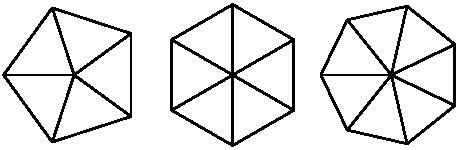
\includegraphics[scale=0.8]{figs/pies.pdf}}
\caption{Torte disegnate con turtle.}
\label{fig.pies}
\end{figure}

\vspace{0.2in}
\begin{exercise}
\index{torta}

Scrivete un insieme di funzioni, generali in modo appropriato, che disegni delle forme a torta come in Figura~\ref{fig.pies}.

Soluzione: \url{http://thinkpython2.com/code/pie.py}.

\end{exercise}

\vspace{0.2in}
\begin{exercise}
\index{alfabeto}
\index{macchina da scrivere a tartaruga}

Le lettere dell'alfabeto possono essere costruite con un moderato numero di elementi di base, come linee orizzontali e verticali e alcune curve. Progettate un alfabeto che possa essere disegnato con un numero minimo di elementi di base e poi scrivete delle funzioni che disegnino le lettere.

Dovreste scrivere una funzione per ogni lettera, con nomi tipo
\verb"disegna_a", \verb"disegna_b", ecc., e inserirle in un file di nome {\tt lettere.py}.  Potete scaricare una ``macchina da scrivere a tartaruga'' da \url{http://thinkpython2.com/code/typewriter.py}
per aiutarvi a provare il vostro codice.

Soluzione: \url{http://thinkpython2.com/code/letters.py}, richiede anche
\url{http://thinkpython2.com/code/polygon.py}.

\end{exercise}

\vspace{0.2in}
\begin{exercise}

Documentatevi sulle spirali sul sito \url{http://it.wikipedia.org/wiki/Spirale}; quindi scrivete un programma che disegni una spirale di Archimede (o di qualche altro tipo).  Soluzione: \url{http://thinkpython2.com/code/spiral.py}.
\index{spirale}
\index{spirale di Archimede} 

\end{exercise}


\chapter{Istruzioni condizionali e ricorsione}

L'argomento principale di questo capitolo è l'istruzione {\tt if}, che permette di eseguire codice diverso a seconda dello stato del programma. Prima di tutto, vediamo però due nuovi operatori: divisione intera e modulo.

\section{Divisione intera e modulo}

L'operatore di {\bf divisione intera}, \verb"//", divide due numeri e arrotonda il risultato all'intero inferiore. Ad esempio, supponiamo che la durata di un film sia di 105 minuti, e di volerla esprimere in ore. La normale divisione  restituisce un numero decimale:

\begin{verbatim}
>>> minuti = 105
>>> minuti / 60
1.75
\end{verbatim}

Ma di solito non si esprimono le ore con un numero decimale. La divisione intera dà invece come risultato il numero di ore, arrotondando per difetto:

\begin{verbatim}
>>> minuti = 105
>>> ore = minuti // 60
>>> ore
1
\end{verbatim}

Per ottenere il resto, potete sottrarre dai minuti l'equivalente delle ore:

\begin{verbatim}
>>> resto = minuti - ore * 60
>>> resto
45
\end{verbatim}

\index{divisione!intera}
\index{divisione!decimale}
\index{modulo, operatore}
\index{operatore!modulo}

Come alternativa si può utilizzare l'{\bf operatore modulo}, \verb"%", che 
restituisce il resto dell'operazione di divisione tra due numeri interi.

\begin{verbatim}
>>> resto = minuti % 60
>>> resto
45
\end{verbatim}
%

L'operatore modulo è più utile di quel che sembra. Per esempio, vi permette di controllare se un numero intero è divisibile per un altro: se
{\tt x \% y} è zero, significa che {\tt x} è divisibile per {\tt y}.
\index{divisibilità}

Potete inoltre estrarre la cifra più a destra o più cifre di un numero. Ad esempio {\tt x \% 10} restituisce la cifra più a destra di {\tt x} (in base 10). E analogamente, {\tt x \% 100} restituisce le ultime due cifre.

Per chi usa Python 2, la divisione funziona in modo diverso. L'operatore di divisione intera non esiste, e quello di divisione, \verb"/", esegue una divisione intera se entrambi gli operandi sono interi, mentre il risultato è un decimale a virgola mobile se almeno uno degli operandi è un decimale.
\index{Python 2}


\section{Espressioni booleane}
\index{espressione!booleana}
\index{operatore!logico}

Un'{\bf espressione booleana} è un'espressione che può essere o vera o falsa.  Gli esempi che seguono usano l'operatore {\tt ==}, confrontano due valori e restituiscono {\tt True} (vero) se sono uguali, {\tt False} (falso) altrimenti:

\begin{verbatim}
>>> 5 == 5
True
>>> 5 == 6
False
\end{verbatim}
%
{\tt True} e {\tt False} sono valori speciali che sono di tipo {\tt bool}; non sono delle stringhe:
\index{True, valore speciale}
\index{False, valore speciale}
\index{valore speciale!True}
\index{valore speciale!False}
\index{bool, tipo}
\index{tipo!bool}

\begin{verbatim}
>>> type(True)
<class 'bool'>
>>> type(False)
<class 'bool'>
\end{verbatim}
%
L'operatore {\tt ==} è uno degli {\bf operatori di confronto} (chiamati anche operatori relazionali); gli altri sono:

\begin{verbatim}
      x != y               # x è diverso da y
      x > y                # x è maggiore di y
      x < y                # x è minore di y
      x >= y               # x è maggiore o uguale a y
      x <= y               # x è minore o uguale a y
\end{verbatim}
%
Queste operazioni vi saranno familiari, tuttavia i simboli usati in Python non sono del tutto uguali a quelli matematici. Un errore frequente è usare il simbolo di uguale({\tt =}) anziché il doppio uguale ({\tt ==}). Ricordatevi la differenza: {\tt =} è un operatore di assegnazione, mentre {\tt ==} è un operatore di confronto. Inoltre in Python non esistono simboli come {\tt =<} o {\tt =>}.
\index{confronto, operatore di}
\index{operatore!confronto}


\section {Operatori logici}
\index{logico, operatore}
\index{operatore!logico}

Ci sono tre {\bf operatori logici}: {\tt and}, {\tt
or}, e {\tt not}.  Il significato di questi operatori è simile a quello comune (e, o, non): per esempio, l'espressione {\tt x > 0 and x < 10} è vera solo se sono vere {\em entrambe} le condizioni, cioè {\tt x} è più grande di 0 {\em e} più piccolo di 10.
\index{and, operatore}
\index{or, operatore}
\index{not, operatore}
\index{operatore!and}
\index{operatore!or}
\index{operatore!not}

L'espressione {\tt n \% 2 == 0 or n \% 3 == 0} invece è vera se è verificata {\em almeno una} delle due condizioni, cioè se il numero è divisibile per 2 {\em o} per 3 (o per entrambi).

Infine, l'operatore {\tt not} nega il valore di un'espressione booleana, per cui {\tt not (x > y)} è vera se {\tt x > y} è falsa, cioè se {\tt x} è minore o uguale a {\tt y}.

In senso stretto, gli operandi degli operatori logici dovrebbero essere delle espressioni booleane, ma qui Python non è rigido: ogni numero diverso da zero viene accettato ed interpretato come {\tt True}.

\begin{verbatim}
>>> 42 and True
True
\end{verbatim}
%
Questa flessibilità può essere utile, ma ci sono alcune sottigliezze che potrebbero confondere. È preferibile evitarla (a meno che non sappiate esattamente quello che state facendo).


\section{Esecuzione condizionale}
\label{conditional.execution}

\index{istruzione!condizionale}
\index{if, istruzione}
\index{istruzione!if}
\index{esecuzione condizionale}
Se volete scrivere programmi utili, vi capiterà spesso di dover controllare se si verificano determinate condizioni, e di variare di conseguenza il comportamento del programma. Le {\bf istruzioni condizionali} servono proprio a questo. La forma più semplice di istruzione condizionale è l'istruzione {\tt if} (``se'' in inglese):

\begin{verbatim}
if x > 0:
    print('x è positivo')
\end{verbatim}
%
L'espressione booleana dopo l'istruzione {\tt if} è chiamata {\bf condizione}.  Se risulta vera, viene eseguita l'istruzione indentata che segue sulla riga successiva. Altrimenti, non succede nulla.
\index{condizione}
\index{istruzione!composta}

L'istruzione {\tt if} ha la stessa struttura che abbiamo già visto nel caso delle definizioni di funzione: un'intestazione seguita da un corpo indentato. Le istruzioni come questa vengono chiamate {\bf istruzioni composte}.

Non c'è limite al numero di istruzioni che possono essere scritte nel corpo, ma deve sempre essercene almeno una. Talvolta può servire che il corpo sia privo di istruzioni (di solito quando c'è del codice ancora da scrivere); in questo caso potete usare l'istruzione {\tt pass}, che serve solo da segnaposto temporaneo e nulla più:
\index{pass, istruzione}
\index{istruzione!pass}

\begin{verbatim}
if x < 0:
    pass          # scrivere cosa fare con i valori negativi!
\end{verbatim}
%

\section{Esecuzione alternativa}
\label{alternative.execution}
\index{esecuzione alternativa}
\index{else, parola chiave}
\index{parola chiave!else}

Una seconda forma di istruzione {\tt if} è l'{\bf esecuzione alternativa},
dove esistono due possibili azioni, e il valore della condizione determina quale delle due azioni debba essere eseguita e quale no. La sintassi è:

\begin{verbatim}
if x % 2 == 0:
    print('x è pari')
else:
    print('x è dispari')
\end{verbatim}
%
Se il resto della divisione di {\tt x} per 2 è zero, significa che {\tt x} è un numero pari, e il programma mostra il messaggio appropriato. Altrimenti (\verb"else"), se la condizione è falsa, viene eseguito il secondo blocco di istruzioni. Dato che la condizione deve essere necessariamente o vera o falsa, sarà sempre eseguita una sola delle due alternative. Queste sono dette {\bf ramificazioni}, perché rappresentano dei bivi nel flusso di esecuzione del programma.
\index{ramificazione}


\section{Condizioni in serie}
\index{serie, condizioni in}
\index{condizione!in serie}

A volte è necessario considerare più di due possibili sviluppi, e occorre che nel programma ci siano più di due ramificazioni. Un modo per esprimere questo tipo di calcolo sono le {\bf condizioni in serie}:

\begin{verbatim}
if x < y:
    print('x è minore di y')
elif x > y:
    print('x è maggiore di y')
else:
    print('x e y sono uguali')
\end{verbatim}
%
{\tt elif} è l'abbreviazione di {\em else if}, che in inglese significa ``altrimenti se''. Anche stavolta verrà eseguito solo uno dei tre rami, a seconda dell'esito del confronto tra {\tt x} e {\tt y}. Non c'è alcun limite al numero di istruzioni {\tt elif}. Se esiste una clausola {\tt else}, deve essere scritta per ultima, ma non è obbligatoria; il ramo corrispondente viene eseguito solo quando tutte le condizioni precedenti sono false.
\index{elif, parola chiave }
\index{parola chiave!elif}


\begin{verbatim}
if scelta == 'a':
    disegna_a()
elif scelta == 'b':
    disegna_b()
elif scelta == 'c':
    disegna_c()
\end{verbatim}
%
Le condizioni vengono controllate nell'ordine dall'alto al basso: se la prima è falsa, viene controllata la seconda e così via. Non appena una condizione risulta vera, viene eseguito il ramo corrispondente e l'istruzione termina. Anche se risultassero vere altre condizioni successive, viene eseguita sempre e soltanto la prima che risulta vera.  


\section{Condizioni nidificate}
\index{condizione!nidificata}

Si può anche inserire un'istruzione condizionale nel corpo di un'altra istruzione condizionale. Possiamo dunque scrivere l'esempio del paragrafo precedente anche in questo modo:

\begin{verbatim}
if x == y:
    print('x e y sono uguali')
else:
    if x < y:
        print('x è minore di y')
    else:
        print('x è maggiore di y')
\end{verbatim}
%
La condizione più esterna contiene due rami: il primo contiene un'istruzione semplice, il secondo un'altra istruzione {\tt if} che a sua volta ha due ramificazioni. Entrambi i rami del secondo {\tt if} sono istruzioni di stampa, ma potrebbero anche contenere a loro volta ulteriori istruzioni condizionali.

Anche se l'indentazione delle istruzioni aiuta ad evidenziare la struttura, le {\bf condizioni nidificate} diventano rapidamente difficili da leggere, quindi è meglio usarle con moderazione.

Gli operatori logici permettono spesso di semplificare le istruzioni condizionali nidificate. Il codice seguente può essere riscritto usando un'unica condizione:

\begin{verbatim}
if 0 < x:
    if x < 10:
        print('x è un numero positivo a una cifra.')
\end{verbatim}
%
Infatti, dato che l'istruzione di stampa è eseguita solo se si verificano entrambe le condizioni, possiamo ottenere lo stesso risultato usando l'operatore {\tt and}:

\begin{verbatim}
if 0 < x and x < 10:
    print('x è un numero positivo a una cifra.')
\end{verbatim}

Per una condizione di questo tipo, Python consente anche un'opzione sintattica più concisa:

\begin{verbatim}
if 0 < x < 10:
    print('x è un numero positivo a una cifra.')
\end{verbatim}


\section{Ricorsione}
\label{recursion}
\index{ricorsione}

Abbiamo visto che è del tutto normale che una funzione ne chiami un'altra, ma è anche consentito ad una funzione di chiamare se stessa. L'utilità può non essere immediatamente comprensibile, ma questa è una delle cose più magiche che un programma possa fare. Per fare un esempio, diamo un'occhiata a questa funzione:

\begin{verbatim}
def contoallarovescia(n):
    if n <= 0:
        print('Via!')
    else:
        print(n)
        contoallarovescia(n-1)
\end{verbatim}
%
Se {\tt n} vale 0 o è negativo, la funzione scrive la parola ``Via!''.
Altrimenti scrive il numero {\tt n} e poi chiama la funzione {\tt
contoallarovescia} (cioè se stessa) passando un argomento che vale {\tt n-1}.

Cosa succede quando chiamiamo la funzione in questo modo?

\begin{verbatim}
>>> contoallarovescia(3)
\end{verbatim}
%
L'esecuzione di {\tt contoallarovescia} inizia da {\tt n=3}, e dato che
{\tt n} è maggiore di 0, stampa il valore 3, poi chiama se stessa...

\begin{quote}
L'esecuzione di {\tt contoallarovescia} inizia da {\tt n=2}, e dato che
{\tt n} è maggiore di 0, stampa il valore 2, poi chiama se stessa...

\begin{quote}
L'esecuzione di {\tt contoallarovescia} inizia da {\tt n=1}, e dato che
{\tt n} è maggiore di 0, stampa il valore 1, poi chiama se stessa...

\begin{quote}
L'esecuzione di {\tt contoallarovescia} inizia da {\tt n=0}, e dato che {\tt
n} è uguale a 0, stampa la parola ``Via!'' e poi ritorna.
\end{quote}

La funzione {\tt contoallarovescia} che aveva dato {\tt n=1} ritorna.
\end{quote}

La funzione {\tt contoallarovescia} che aveva dato {\tt n=2} ritorna.
\end{quote}

La funzione {\tt contoallarovescia} che aveva dato {\tt n=3} ritorna.

E infine ritorniamo in \verb"__main__". Il risultato finale è questo:
\index{main}

\begin{verbatim}
3
2
1
Via!
\end{verbatim}
%
Una funzione che chiama se stessa si dice {\bf ricorsiva} e la procedura che la esegue è detta {\bf ricorsione}.
\index{ricorsione}
\index{funzione!ricorsiva}

Come secondo esempio, scriviamo una funzione che stampi una data stringa per {\tt n} volte.

\begin{verbatim}
def stampa_n(s, n):
    if n <= 0:
        return
    print(s)
    stampa_n(s, n-1)
\end{verbatim}
%
Se {\tt n <= 0} l'{\bf istruzione di ritorno} {\tt return} provoca l'uscita dalla funzione. Il flusso dell'esecuzione torna immediatamente al chiamante, e le righe rimanenti della funzione non vengono eseguite.
\index{return, istruzione}
\index{istruzione!return}

Il resto della funzione è simile a {\tt contoallarovescia}: visualizza la stringa {\tt s} e chiama se stessa per $n-1$ altre volte. Il numero di righe risultanti sarà {\tt 1 + (n - 1)}, che corrisponde a
{\tt n}.

Per esempi semplici come questi, è forse più facile usare un ciclo {\tt
for}. Vedremo però più avanti degli esempi difficili da scrivere con un ciclo {\tt for} ma facili con la ricorsione; meglio quindi cominciare subito a prendere mano.
\index{for, ciclo}
\index{ciclo!for}


\section{Diagrammi di stack delle funzioni ricorsive}
\label{recursive.stack}
\index{diagramma!di stack}
\index{funzione!frame di}
\index{frame}

Nel Paragrafo~\ref{stackdiagram}, abbiamo usato un diagramma di stack per raffigurare lo stato di un programma nel corso di una chiamata di funzione. Lo stesso tipo di diagramma può servire a capire come lavora una funzione ricorsiva.

Ad ogni chiamata di funzione, Python crea un frame che contiene le variabili locali interne alla funzione ed i suoi parametri. Nel caso di una funzione ricorsiva, possono esserci contemporaneamente più frame della stessa funzione nello stack.

La Figura~\ref{fig.stack2} mostra il diagramma di stack della funzione {\tt contoallarovescia} chiamata con {\tt n = 3}.

\begin{figure}
\centerline
{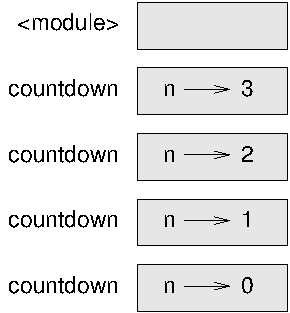
\includegraphics[scale=0.8]{figs/stack2.pdf}}
\caption{Diagramma di stack.}
\label{fig.stack2}
\end{figure}

Come al solito, il livello superiore dello stack è il frame di \verb"__main__", che
è vuoto, perché non vi abbiamo creato alcuna variabile né gli abbiamo passato alcun argomento.
\index{caso base}
\index{ricorsione!caso base}

Nei quattro frame di {\tt contoallarovescia}, il parametro {\tt n} ha valori differenti. Il livello inferiore dello stack, dove {\tt n=0}, è chiamato {\bf caso base}. Quest'ultimo non effettua ulteriori chiamate ricorsive, quindi non produce ulteriori frame.

Come esercizio, disegnate il diagramma di stack della funzione \verb"stampa_n" chiamata con \verb"s='Ciao'" e {\tt n=2}. Poi, scrivete una funzione di nome \verb"fai_n" che accetti come argomenti un oggetto funzione e un numero {\tt n}, e che chiami per {\tt n} volte la funzione data.


\section{Ricorsione infinita}
\index{ricorsione!infinita}
\index{errore!in esecuzione}

\index{traceback}

Se una ricorsione non raggiunge mai un caso base, continua ad effettuare chiamate ricorsive all'infinito e il programma non può terminare. Questa situazione è nota come {\bf ricorsione infinita}, e di solito non è considerata un fatto positivo.
Ecco un programma minimale che genera una ricorsione infinita:

\begin{verbatim}
def ricorsiva():
    ricorsiva()
\end{verbatim}
%
Nella maggior parte degli ambienti di programmazione, un programma con una ricorsione infinita non viene eseguito davvero all'infinito. Python mostra un messaggio di errore quando viene raggiunto il massimo livello di ricorsione consentito:
\index{eccezione!RuntimeError}
\index{RuntimeError}

\begin{verbatim}
  File "<stdin>", line 2, in ricorsiva
  File "<stdin>", line 2, in ricorsiva
  File "<stdin>", line 2, in ricorsiva
                  .   
                  .
                  .
  File "<stdin>", line 2, in ricorsiva
RuntimeError: Maximum recursion depth exceeded
\end{verbatim}
%
Questo traceback è un po' più grande di quello che abbiamo visto nel capitolo precedente. Quando si verifica l'errore, nello stack ci sono oltre 1000 frame di {\tt ricorsiva}!

Se vi imbattete accidentalmente in una ricorsione infinita, rivedete la vostra funzione per accertare che esista un caso base che non genera una ulteriore chiamata ricorsiva. E se c'è un caso base, controllate che venga sicuramente raggiunto.

\section{Input da tastiera}
\index{Input da tastiera}

I programmi che abbiamo scritto finora non accettano dati in ingresso da parte dell'utente, ed eseguono sempre le stesse operazioni.

In Python esiste una funzione predefinita chiamata \verb"input" che sospende il programma ed attende che l'utente scriva qualcosa. Quando l'utente preme il tasto {\sf Invio} oppure {\sf Enter}, il programma riprende e \verb"input" restituisce quello che l'utente ha inserito, come stringa. In Python 2, la funzione si chiama invece \verb"raw_input" .
\index{Python 2}
\index{input, funzione}
\index{funzione!input}

\begin{verbatim}
>>> testo = input()
Cosa stai aspettando?
>>> testo
'Cosa stai aspettando?'
\end{verbatim}
%
Prima dell'inserimento dei dati, è buona norma visualizzare un messaggio, chiamato prompt, che informa l'utente di ciò che deve inserire. A questo scopo, \verb"input" accetta un prompt come argomento:
\index{prompt}

\begin{verbatim}
>>> nome = input('Come...ti chiami?\n')
Come...ti chiami?
Artù, Re dei Bretoni!
>>> nome
'Artù, Re dei Bretoni!'
\end{verbatim}
%
La sequenza \verb"\n" alla fine del prompt rappresenta un {\bf ritorno a capo},
un carattere speciale che provoca un'interruzione di riga. Ecco perché l'input dell'utente compare sulla riga successiva sotto al prompt.
\index{ritorno a capo}

Se l'input atteso deve essere un numero intero, si può provare a convertire il valore inserito in {\tt int}:

\begin{verbatim}
>>> prompt = 'Qual è la velocità in volo di una rondine?\n'
>>> velocita = input(prompt)
Qual è la velocità in volo di una rondine?
42
>>> int(velocita)
42
\end{verbatim}
%
Ma se la stringa inserita contiene qualcosa di diverso da dei valori numerici, si verifica un errore:

\begin{verbatim}
>>> velocita = input(prompt)
Qual è la velocità in volo di una rondine?
Cosa intendi, una rondine europea o africana?
>>> int(velocita)
ValueError: invalid literal for int() with base 10
\end{verbatim}
%
Vedremo più avanti come trattare questo tipo di errori.
\index{ValueError}
\index{eccezione!ValueError}


\section{Debug}
\label{whitespace}
\index{debug}
\index{traceback}

Quando si verifica un errore di sintassi o di runtime, il messaggio d'errore  contiene molte informazioni, ma può essere sovrabbondante. Di solito le parti più utili sono:

\begin{itemize}

\item Che tipo di errore era, e

\item Dove si è verificato.

\end{itemize}

Gli errori di sintassi di solito sono facili da trovare, con qualche eccezione. Gli spaziatori possono essere insidiosi, perché spazi e tabulazioni non sono visibili e non siamo abituati a tenerne conto.
\index{spaziatore}

\begin{verbatim}
>>> x = 5
>>>  y = 6
  File "<stdin>", line 1
    y = 6
    ^
IndentationError: unexpected indent
\end{verbatim}
%
In questo esempio, il problema è che la seconda riga è erroneamente indentata di uno spazio, mentre dovrebbe stare al margine sinistro. Ma il messaggio di errore punta su {\tt y}, portando fuori strada. In genere, i messaggi di errore indicano dove il problema è venuto a galla, ma il vero errore potrebbe essere in un punto precedente del codice, a volte anche nella riga precedente.

\index{errore!in esecuzione}

Lo stesso vale per gli errori di runtime. 

Supponiamo di voler calcolare un rapporto segnale/rumore in decibel. La formula è
 $SNR_{db} = 10 \log_{10} (P_{segnale} / P_{rumore})$. In Python si può scrivere:

\begin{verbatim}
import math
potenza_segnale = 9
potenza_rumore = 10
rapporto = potenza_segnale // potenza_rumore
decibel = 10 * math.log10(rapporto)
print(decibel)
\end{verbatim}
%
Se avviate questo programma, compare un messaggio di errore.
\index{eccezione!OverflowError}
\index{OverflowError}

\begin{verbatim}
Traceback (most recent call last):
  File "snr.py", line 5, in ?
    decibel = 10 * math.log10(rapporto)
ValueError: math domain error
\end{verbatim}
%
Il messaggio punta alla riga 5, ma lì non c'è niente di sbagliato. Per trovare il vero errore, può essere utile stampare il valore di {\tt rapporto}, che risulta essere 0. Il problema sta nella riga 4, perché calcola una divisione intera anziché una normale divisione.
\index{divisione!intera}

Prendetevi la briga di leggere attentamente i messaggi di errore, ma non date per scontato che tutto quello che dicono sia esatto.


\section{Glossario}

\begin{description}

\item[divisione intera:] Operatore, che ha per simbolo {\tt //}, che divide due numeri e arrotonda il risultato all'intero inferiore (ovvero, verso l'infinito negativo).
\index{divisione!intera}
  
\item[operatore modulo:]  Operatore matematico, che ha per simbolo ({\tt \%}), che restituisce il resto della divisione tra due operandi interi.
\index{modulo, operatore}
\index{operatore!modulo}

\item[espressione booleana:]  Espressione il cui valore è o vero 
({\tt True}) o falso ({\tt False}).
\index{espressione!booleana}

\item[operatore di confronto:] Operatore che confronta due valori detti operandi: {\tt ==}, {\tt !=}, {\tt >}, {\tt <}, {\tt >=}, e {\tt <=}.

\item[operatore logico:] Operatore che unisce delle espressioni booleane: {\tt and}, {\tt or}, e {\tt not}.

\item[istruzione condizionale:]  Istruzione che controlla il flusso di esecuzione del programma, variandolo a seconda di determinate condizioni.
\index{istruzione!condizionale}

\item[condizione:] Espressione booleana in un'istruzione condizionale che determina quale ramificazione sarà eseguita.
\index{condizione}

\item[istruzione composta:]  Istruzione che consiste di un'intestazione e di un corpo. L'intestazione deve terminare con i due punti (:) e il corpo deve essere indentato rispetto ad essa.
\index{istruzione!composta}

\item[ramificazione:] Uno dei blocchi di istruzioni alternative presenti in un'istruzione condizionale.
\index{ramificazione}

\item[condizioni in serie:]  Istruzione condizionale con una serie di ramificazioni alternative.
\index{condizione!in serie}

\item[condizione nidificata (o annidata):]  Un'istruzione condizionale inserita in una ramificazione di un'altra istruzione condizionale.
\index{condizione!nidificata}

\item[istruzione di ritorno:] Un'istruzione che fa terminare immediatamente una funzione e ritorna al chiamante.

\item[ricorsione:]  Procedura che chiama la stessa funzione attualmente in esecuzione.
\index{ricorsione}

\item[caso base:]  Ramificazione di un'istruzione condizionale, posta in una funzione ricorsiva, che non esegue a sua volta una chiamata ricorsiva.
\index{caso base}

\item[ricorsione infinita:]  Una ricorsione priva di un caso base, oppure che non lo raggiunge mai. Nell'evenienza, causa un errore in esecuzione.
\index{ricorsione!infinita}

\end{description}

\section{Esercizi}

\begin{exercise}

Il modulo {\tt time} contiene una funzione, anch'essa di nome {\tt time}, che restituisce l'attuale GMT (Tempo Medio di Greenwich) riferito ad un ``tempo zero'', che è un momento arbitrario usato come punto di riferimento. Nei sistemi UNIX, questo ``tempo zero'' è il 1 gennaio 1970.

\begin{verbatim}
>>> import time
>>> time.time()
1437746094.5735958
\end{verbatim}

Realizzate uno script che acquisisca il tempo attuale e lo converta in un tempo in ore, minuti e secondi, più i giorni trascorsi dal ``tempo zero''.

\end{exercise}

\vspace{0.2in}
\begin{exercise}
\index{Fermat, ultimo teorema di}

L'ultimo teorema di Fermat afferma che non esistono interi positivi
$a$, $b$, e $c$ tali che

\[ a^n + b^n = c^n \]
%
per qualsiasi valore di $n$ maggiore di 2.

\begin{enumerate}

\item Scrivete una funzione di nome \verb"verifica_fermat" che richieda quattro parametri---{\tt a}, {\tt b}, {\tt c} e {\tt n}---e controlli se il teorema regge. Se $n$ è maggiore di 2 e fosse

\[a^n + b^n = c^n \]
%
il programma dovrebbe visualizzare: ``Santi Numi, Fermat si è sbagliato!'',
altrimenti: ``No, questo non è vero.''

\item Scrivete una funzione che chieda all'utente di inserire valori di {\tt a}, {\tt b}, {\tt c} e {\tt n}, li converta in interi e usi \verb"verifica_fermat" per controllare se violano il teorema di Fermat.

\end{enumerate}

\end{exercise}

\vspace{0.2in}
\begin{exercise}
\index{triangolo}

Dati tre bastoncini, può essere possibile o meno riuscire a sistemarli in modo da formare un triangolo. Per esempio, se uno dei bastoncini misura 12 centimetri e gli altri due 1 centimetro, non riuscirete a far toccare le estremità di tutti e tre i bastoncini. Date tre lunghezze, c'è una semplice regola per controllare se è possibile formare un triangolo:

\begin{quotation}
Se una qualsiasi delle tre lunghezze è maggiore della somma delle altre due, non potete formare un triangolo. (Se la somma di due lunghezze è uguale alla terza, si ha un triangolo ``degenere''.)
\end{quotation}

\begin{enumerate}

\item Scrivete una funzione di nome \verb"triangolo" che riceva tre interi come argomenti e che mostri ``Si''' o ``No'', a seconda che si possa o meno formare un triangolo con dei bastoncini delle tre lunghezze date.

\item Scrivete una funzione che chieda all'utente di inserire tre lunghezze, le converta in interi, e le passi a \verb"triangolo" per verificare se si possa o meno formare un triangolo.

\end{enumerate}

\end{exercise}

\vspace{0.2in}
\begin{exercise}

Qual è l'output del seguente programma?
Disegnate un diagramma di stack che illustri lo stato del programma nel momento in cui stampa il risultato.

\begin{verbatim}
def ricorsione(n, s):
    if n == 0:
        print(s)
    else:
        ricorsione(n-1, n+s)

ricorsione(3, 0)
\end{verbatim}

\begin{enumerate}

\item Cosa succede se chiamate la funzione in questo modo: {\tt ricorsione(-1, 0)}?

\item Scrivete una stringa di documentazione che spieghi tutto quello che serve per usare questa funzione (e niente di più).

\end{enumerate}

\end{exercise}

Gli esercizi seguenti utilizzano il modulo turtle, descritto nel Capitolo~\ref{turtlechap}:
\index{turtle}

\vspace{0.2in}
\begin{exercise}

Leggete la seguente funzione e cercate di capire cosa fa (vedere gli esempi nel Capitolo~\ref{turtlechap}). Quindi eseguitela per controllare se avevate indovinato.

\begin{verbatim}
def disegna(t, lunghezza, n):
    if n == 0:
        return
    angolo = 50
    t.fd(lunghezza*n)
    t.lt(angolo)
    disegna(t, lunghezza, n-1)
    t.rt(2*angolo)
    disegna(t, lunghezza, n-1)
    t.lt(angolo)
    t.bk(lunghezza*n)
\end{verbatim}

\end{exercise}
\begin{figure}
\centerline
{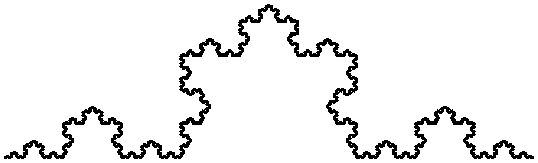
\includegraphics[scale=0.8]{figs/koch.pdf}}
\caption{Una curva di Koch.}
\label{fig.koch}
\end{figure}

\vspace{0.2in}
\begin{exercise}
\index{curva di Koch}

La curva di Koch è un frattale che somiglia a quello in Figura~\ref{fig.koch}.  Per disegnare una curva di Koch di lunghezza $x$, dovete:

\begin{enumerate}

\item Disegnare una curva di Koch di lunghezza $x/3$.

\item Girare a sinistra di 60 gradi.

\item Disegnare una curva di Koch di lunghezza $x/3$.

\item Girare a destra di 120 gradi.

\item Disegnare una curva di Koch di lunghezza $x/3$.

\item Girare a sinistra di 60 gradi.

\item Disegnare una curva di Koch di lunghezza $x/3$.

\end{enumerate}

Ad eccezione di quando $x$ è minore di 3: in questo caso si disegna una linea dritta lunga $x$.

\begin{enumerate}

\item Scrivete una funzione di nome {\tt koch} che preveda una tartaruga e una lunghezza come parametri, e che usi la tartaruga per disegnare una curva di Koch della data lunghezza.

\item Scrivete una funzione chiamata {\tt fioccodineve} che disegni tre curve di Koch per ottenere il contorno di un fiocco di neve.

Soluzione: \url{http://thinkpython2.com/code/koch.py}.

\item La curva di Koch può essere generalizzata in alcuni modi. Consultate 
\url{http://it.wikipedia.org/wiki/Curva_di_Koch} per degli esempi e implementate quello che preferite.

\end{enumerate}
\end{exercise}


\chapter{Funzioni produttive}
\label{fruitchap}

Molte tra le funzioni di Python che abbiamo usato, come quelle matematiche, producono dei valori di ritorno. Ma quelle che abbiamo scritto noi finora sono tutte ``vuote'': hanno un qualche effetto, come visualizzare un testo o muovere tartarughe, ma non hanno un valore di ritorno. In questo capitolo vedremo come si scrivono le funzioni che chiameremo ``produttive''.

\section{Valori di ritorno}
\index{valore di ritorno}

La chiamata di una funzione genera un nuovo valore, che di solito viene associato ad una variabile o si usa come parte di un'espressione.

\begin{verbatim}
e = math.exp(1.0)
altezza = raggio * math.sin(radianti)
\end{verbatim}
%
Le funzioni che abbiamo scritto finora sono ``vuote''. Detto in modo semplicistico, non hanno valore di ritorno; ma a voler essere precisi, il loro valore di ritorno è {\tt None}.

In questo capitolo scriveremo finalmente delle funzioni che restituiscono un valore e che chiameremo funzioni ``produttive''.
Facciamo un primo esempio con {\tt area}, che calcola l'area di un cerchio di dato raggio:

\begin{verbatim}
def area(raggio):
    a = math.pi * raggio**2
    return a
\end{verbatim}
%
Abbiamo già incontrato l'istruzione {\tt return}, ma in una funzione produttiva questa istruzione include un'espressione. Il suo significato è: ``ritorna subito da questa funzione e usa l'espressione seguente come valore di ritorno''. L'espressione può essere anche complessa, e allora possiamo riscrivere la funzione in modo più compatto:
\index{return, istruzione}
\index{istruzione!return}

\begin{verbatim}
def area(raggio):
    return math.pi * raggio**2
\end{verbatim}
%
Peraltro, una {\bf variabile temporanea} come {\tt a} può rendere più agevole il debug.
\index{variabile!temporanea}

Talvolta occorre prevedere più istruzioni di ritorno, una per ciascuna ramificazione di un'istruzione condizionale:

\begin{verbatim}
def valore_assoluto(x):
    if x < 0:
        return -x
    else:
        return x
\end{verbatim}
%
Dato che queste istruzioni {\tt return} si trovano in due rami di una
condizione alternativa, solo una delle due sarà effettivamente eseguita.

Non appena viene eseguita un'istruzione {\tt return}, la funzione termina senza eseguire ulteriori istruzioni. Il codice che viene a trovarsi dopo l'istruzione {\tt return} o in ogni altro punto che non può essere raggiunto dal flusso di esecuzione, è detto {\bf codice morto}.
\index{codice morto}

In una funzione produttiva, occorre accertarsi che ogni possibile percorso del flusso di esecuzione del programma conduca ad un'istruzione {\tt return}. Per esempio:

\begin{verbatim}
def valore_assoluto(x):
    if x < 0:
        return -x
    if x > 0:
        return x
\end{verbatim}
%
Questa funzione ha un difetto, in quanto se {\tt x} è uguale a 0, nessuna delle due condizioni è vera e la funzione termina senza incontrare un'istruzione {\tt return}. Se il flusso di esecuzione arriva alla fine della funzione, il valore di ritorno sarà {\tt None}, che non è di certo il valore assoluto di 0.
\index{None, valore speciale}
\index{valore speciale!None}

\begin{verbatim}
>>> print(valore_assoluto(0))
None
\end{verbatim}
%
A proposito: Python contiene già la funzione {\tt abs} che calcola il valore assoluto.
\index{abs, funzione}
\index{funzione!abs}

Per esercitarvi, scrivete una funzione di nome {\tt compara} che prenda due valori, {\tt x} e {\tt y}, e restituisca
 {\tt 1} se {\tt x > y}, {\tt 0} se {\tt x == y}, e {\tt -1} se {\tt x < y}.
\index{compara, funzione}
\index{funzione!compara}


\section{Sviluppo incrementale}
\label{incremental.development}
\index{tecnica di sviluppo!incrementale}

Scrivendo funzioni di dimensioni sempre maggiori, aumenterà anche il tempo da dedicare al debug.

Per affrontare programmi di complessità crescente, suggerisco una tecnica chiamata {\bf sviluppo incrementale}. Lo scopo dello sviluppo incrementale è evitare lunghe sessioni di debug, aggiungendo e provando solo piccole parti di codice alla volta.
\index{test!sviluppo incrementale}
\index{teorema di Pitagora}

Come esempio, supponiamo di voler trovare la distanza tra due punti, note le coordinate $(x_1, y_1)$ e $(x_2, y_2)$.
Per il teorema di Pitagora, la distanza è:

\begin{displaymath}
\mathrm{distanza} = \sqrt{(x_2 - x_1)^2 + (y_2 - y_1)^2}
\end{displaymath}
%
Per prima cosa dobbiamo considerare quale interfaccia deve avere in Python la funzione {\tt distanza}. In altre parole, quali sono i dati in ingresso (cioè i parametri), e cosa deve restituire in uscita (cioè il valore di ritorno).

Nel nostro caso, i dati di ingresso (o di {\em input}) sono i due punti, rappresentabili attraverso le loro coordinate (due coppie di numeri); il risultato (o {\em output}) è la distanza, espressa con un valore decimale.

Si può subito scrivere un primo abbozzo di funzione:

\begin{verbatim}
def distanza(x1, y1, x2, y2):
    return 0.0
\end{verbatim}
%
Ovviamente questa prima stesura non calcola ancora la distanza, ma restituisce sempre 0. Però è già una funzione sintatticamente corretta e può essere eseguita: potete quindi provarla prima di procedere a renderla più complessa.

Proviamo allora la nuova funzione, chiamandola con dei valori di esempio:

\begin{verbatim}
>>> distanza(1, 2, 4, 6)
0.0
\end{verbatim}
%
Ho scelto questi valori in modo che la loro distanza orizzontale sia 3 e quella verticale 4. In tal modo, il risultato è pari a 5: l'ipotenusa di un triangolo rettangolo i cui cateti sono lunghi 3 e 4. Quando proviamo una funzione è sempre utile sapere prima il risultato.
\index{test!sapere il risultato}

A questo punto, abbiamo verificato che la funzione è sintatticamente corretta e possiamo cominciare ad aggiungere righe di codice nel corpo. Un passo successivo plausibile è quello di calcolare le differenze $x_2 - x_1$ e $y_2 - y_1$.  Nella nuova versione assegneremo queste differenze a due variabili temporanee e le visualizzeremo.

\begin{verbatim}
def distanza(x1, y1, x2, y2):
    dx = x2 - x1
    dy = y2 - y1
    print('dx è ', dx)
    print('dy è ', dy)
    return 0.0
\end{verbatim}
%
Se la funzione è giusta, usando gli stessi valori di prima dovrebbe mostrare \verb"dx è 3" e \verb"dy è 4". Se le cose stanno così, siamo certi che la funzione si comporta in maniera corretta sia nel ricevere gli argomenti che nell'elaborazione dei primi calcoli. In caso contrario, dovremo comunque controllare solo poche righe.

Procediamo calcolando la somma dei quadrati di {\tt dx} e {\tt dy}:

\begin{verbatim}
def distanza(x1, y1, x2, y2):
    dx = x2 - x1
    dy = y2 - y1
    dsquadr = dx**2 + dy**2
    print('dsquadr è: ', dsquadr)
    return 0.0
\end{verbatim}
%
Di nuovo, eseguiamo il programma in questa fase e controlliamo il risultato, che nel nostro caso dovrebbe essere 25.
Infine, usiamo la funzione radice quadrata {\tt math.sqrt} per calcolare e restituire il risultato:
\index{sqrt, funzione}
\index{funzione!sqrt}

\begin{verbatim}
def distanza(x1, y1, x2, y2):
    dx = x2 - x1
    dy = y2 - y1
    dsquadr = dx**2 + dy**2
    risultato = math.sqrt(dsquadr)
    return risultato
\end{verbatim}
%
Se tutto funziona, abbiamo finito. Altrimenti, possiamo stampare per verifica il valore di {\tt risultato} prima dell'istruzione {\tt return}.

La versione definitiva della funzione non deve mostrare nulla quando viene eseguita; deve  solo restituire un valore. Le istruzioni di stampa che avevamo inserito erano utili per il debug, ma una volta verificato che tutto funziona vanno rimosse. Pezzi di codice temporaneo come questi sono detti {\bf ``impalcature''}, perché sono di aiuto nella fase di costruzione del programma ma non fanno parte del prodotto finale. 
\index{impalcatura}

Quando si inizia a programmare, è bene aggiungere solo poche righe di codice alla volta. Poi, con l'esperienza, potrete scrivere e fare il debug di blocchi di codice sempre più corposi. In ogni caso, la tecnica di sviluppo incrementale potrà farvi risparmiare un bel po' di tempo di debug.

Ecco i punti chiave di questa tecnica:

\begin{enumerate}

\item Iniziare con un programma che funziona e fare ogni volta piccole aggiunte. Ad ogni passo, se dovesse esserci un errore, avrete già idea di dove potrebbe trovarsi.

\item Assegnare i valori intermedi a delle variabili temporanee, così da poterli visualizzare e controllare.

\item Una volta ottenuto un programma funzionante, rimuovere le istruzioni temporanee e consolidare le istruzioni multiple in espressioni composte, a meno che il programma non diventi troppo difficile da leggere.

\end{enumerate}


Come esercizio, usate lo sviluppo incrementale per scrivere una funzione
di nome {\tt ipotenusa}, che restituisca la lunghezza dell'ipotenusa di un
triangolo rettangolo, date le lunghezze dei cateti come argomenti.
Prendete nota di ogni passo del processo di sviluppo man mano che procedete.
\index{ipotenusa}

\section{Composizione}
\index{composizione}
\index{funzione!composizione di}

Come avrete intuito, è possibile chiamare una funzione dall'interno di un'altra funzione. Scriveremo come esempio una funzione che prende due punti geometrici, il centro di un cerchio ed un punto sulla sua circonferenza, e calcola l'area del cerchio.

Supponiamo che le coordinate del centro del cerchio siano memorizzate nelle variabili {\tt xc} e {\tt yc}, e quelle del punto sulla circonferenza in {\tt xp} e {\tt yp}. Innanzitutto, bisogna trovare il raggio del cerchio, che è pari alla distanza tra i due punti. La funzione {\tt distanza} che abbiamo appena scritto, ci torna utile:

\begin{verbatim}
raggio = distanza(xc, yc, xp, yp)
\end{verbatim}
%
Il passo successivo è trovare l'area del cerchio di quel raggio; anche questa funzione l'abbiamo già scritta:

\begin{verbatim}
risultato = area(raggio)
\end{verbatim}
%
Incapsulando il tutto in una sola funzione otteniamo:
\index{incapsulamento}

\begin{verbatim}
def area_cerchio(xc, yc, xp, yp):
    raggio = distanza(xc, yc, xp, yp)
    risultato = area(raggio)
    return risultato
\end{verbatim}
%
Le variabili temporanee {\tt raggio} e {\tt risultato} sono utili per lo sviluppo
e il debug ma, una volta constatato che il programma funziona, possiamo riscrivere la funzione in modo più conciso componendo le chiamate di funzione:

\begin{verbatim}
def area_cerchio(xc, yc, xp, yp):
    return area(distanza(xc, yc, xp, yp))
\end{verbatim}
%

\section{Funzioni booleane}
\label{boolean}

Le funzioni possono anche restituire valori booleani (vero o falso), cosa che è spesso utilizzata per includere al loro interno dei test, anche complessi.  
\index{funzione!booleana}
Per esempio:

\begin{verbatim}
def divisibile(x, y):
    if x % y == 0:
        return True
    else:
        return False
\end{verbatim}
%
È prassi assegnare come nomi alle funzioni booleane dei predicati che, con accezione interrogativa, attendono una risposta sì/no; \verb"divisibile" restituisce {\tt True} o {\tt False} per rispondere alla domanda se è vero o no che {\tt x} è divisibile per {\tt y}.

Facciamo un esempio:

\begin{verbatim}
>>> divisibile(6, 4)
False
>>> divisibile(6, 3)
True
\end{verbatim}
%
Possiamo scrivere la funzione in modo ancora più conciso, in quanto il risultato dell'operatore di confronto {\tt ==} è anch'esso un booleano, restituendolo direttamente:

\begin{verbatim}
def divisibile(x, y):
    return x % y == 0
\end{verbatim}
%
Le funzioni booleane sono usate spesso nelle istruzioni condizionali:
\index{istruzione!condizionale}

\begin{verbatim}
if divisibile(x, y):
    print('x è divisibile per y')
\end{verbatim}
%
Potreste anche scrivere in questo modo:

\begin{verbatim}
if divisibile(x, y) == True:
    print('x è divisibile per y')
\end{verbatim}
%
ma il confronto supplementare è superfluo.

Scrivete ora, per esercizio, una funzione \verb"compreso_tra(x, y, z)" che restituisca {\tt True} se $x \le y \le z$ o {\tt False} altrimenti.


\section{Altro sulla ricorsione}
\label{more.recursion}
\index{ricorsione}
\index{linguaggio!completo di Turing}
\index{Turing, Alan}
\index{Tesi di Turing}

Abbiamo trattato solo una piccola parte di Python, ma è interessante sapere che questo sottoinsieme costituisce un linguaggio di programmazione {\em completo}, vale a dire che tutto ciò che è calcolabile può essere espresso con questo linguaggio. Qualsiasi programma esistente potrebbe essere scritto usando solo le caratteristiche del linguaggio che avete appreso finora (a dire il vero, servirebbe anche qualche altro comando per controllare i dispositivi come mouse, dischi, ecc.).

La prova di questa affermazione è un compito tutt'altro che banale svolto per la prima volta da Alan Turing, uno dei pionieri dell'informatica (qualcuno puntualizzerebbe che era un matematico, ma molti dei primi informatici erano dei matematici). Per questo motivo, è detto Tesi di Turing.
Per una trattazione più completa (ed accurata) della Tesi di Turing, consiglio il libro di Michael Sipser, {\em Introduction to the Theory of Computation}.

Per darvi un'idea di ciò che potete fare con gli strumenti imparati finora, analizziamo alcune funzioni matematiche definite ricorsivamente. Una funzione ricorsiva è una sorta di definizione circolare, cioè la sua definizione contiene un riferimento alla cosa che si sta definendo. Una definizione circolare propriamente detta, non è certo utile:

\begin{description}

\item[vorpale:] aggettivo usato per descrivere qualcosa di vorpale.
\index{vorpale}
\index{definizione!circolare}

\end{description}

Sarebbe fastidioso trovare una definizione simile in un vocabolario.
D'altra parte, se andate a vedere la definizione della funzione fattoriale, che è indicata dal simbolo, $!$), trovate qualcosa del genere:

%
\begin{eqnarray*}
&&  0! = 1 \\
&&  n! = n (n-1)!
\end{eqnarray*}
%
Questa definizione afferma che il fattoriale di 0 è 1 e che il fattoriale di ogni altro valore $n$, è $n$ moltiplicato per il fattoriale di $n-1$.

Pertanto, $3!$ è 3 moltiplicato $2!$, che a sua volta è 2 moltiplicato $1!$, che
   a sua volta è 1 moltiplicato $0!$ (cioè 1). Riassumendo il tutto, $3!$ è uguale a 3 per 2 per 1 per 1, che fa 6.
\index{fattoriale, funzione}
\index{funzione!fattoriale}
\index{definizione!ricorsiva}

Se potete scrivere una definizione ricorsiva di qualcosa, potete anche scrivere un programma Python per valutarla. Per prima cosa occorre individuare quali parametri deve avere la funzione. Il {\tt fattoriale} ha evidentemente un solo parametro, un intero:

\begin{verbatim}
def fattoriale(n):
\end{verbatim}
%
Se l'argomento è 0, dobbiamo solo restituire il valore 1:

\begin{verbatim}
def fattoriale(n):
    if n == 0:
        return 1
\end{verbatim}
%
Altrimenti, e qui viene il bello, dobbiamo fare una chiamata ricorsiva per trovare il fattoriale di $n-1$ e poi moltiplicare questo valore per $n$:

\begin{verbatim}
def fattoriale(n):
    if n == 0:
        return 1
    else:
        ricors = fattoriale(n-1)
        risultato = n * ricors
        return risultato
\end{verbatim}
%
Il flusso di esecuzione del programma è simile a quello di {\tt
contoallarovescia} del Paragrafo~\ref{recursion}. Se chiamiamo {\tt fattoriale}
con il valore 3:

Dato che 3 è diverso da 0, seguiamo il secondo ramo e calcoliamo il fattoriale
   di {\tt n-1}...

\begin{quote}
Dato che 2 è diverso da 0, seguiamo il secondo ramo e calcoliamo il fattoriale di {\tt n-1}...


  \begin{quote}
  Dato che 1 è diverso da 0, seguiamo il secondo ramo e calcoliamo il fattoriale di {\tt n-1}...


    \begin{quote}
    Dato che 0 è uguale a 0, seguiamo il primo ramo e ritorniamo 1 senza fare altre chiamate ricorsive.
    \end{quote}


  Il valore di ritorno (1) è moltiplicato per $n$, che è 1, e il risultato
     ritorna al chiamante.
  \end{quote}


Il valore di ritorno (1) è moltiplicato per $n$, che è 2, e il risultato
     ritorna al chiamante.
\end{quote}


Il valore di ritorno (2) è moltiplicato per $n$, che è 3, e il risultato, 6, diventa il valore di ritorno della chiamata di funzione che ha fatto partire l'intera procedura.
\index{diagramma!di stack}

La Figura~\ref{fig.stack3} mostra il diagramma di stack per tutta questa sequenza di chiamate di funzione:

\begin{figure}
\centerline
{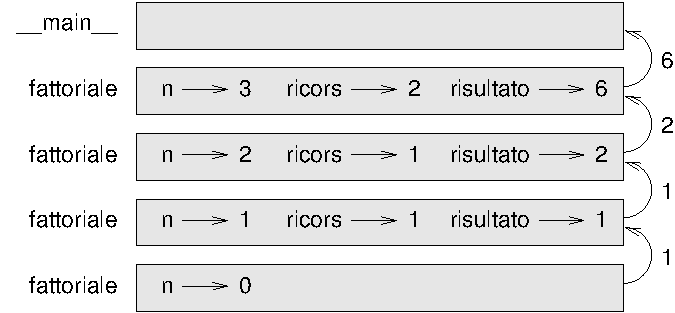
\includegraphics[scale=0.8]{figs/stack3.pdf}}
\caption{Diagramma di stack .}
\label{fig.stack3}
\end{figure}

I valori di ritorno sono illustrati mentre vengono passati all'indietro verso l'alto della pila. In ciascun frame, il valore di ritorno è quello di {\tt risultato}, che è il prodotto di {\tt n} e {\tt ricors}.
\index{funzione!frame di}
\index{frame}

Notate che nell'ultimo frame le variabili locali {\tt ricors} e {\tt risultato} non esistono, perché il ramo che le crea non viene eseguito.


\section{Salto sulla fiducia}
\index{ricorsione}
\index{salto sulla fiducia}

Seguire il flusso di esecuzione è il modo giusto di leggere i programmi, ma
può diventare rapidamente labirintico se le dimensioni del codice aumentano. Un metodo alternativo è quello che io chiamo ``salto sulla fiducia''.  Quando arrivate ad una chiamata di funzione, invece di seguire il flusso di esecuzione, {\em date per scontato} che la funzione chiamata si comporti correttamente e che restituisca il valore esatto.

Nei fatti, già praticate questo atto di fede quando utilizzate le funzioni predefinite: se chiamate {\tt math.cos} o {\tt math.exp}, non andate a controllare il corpo di quelle funzioni: date per scontato che funzionino a dovere perché quelli che hanno scritto le funzioni predefinite sono senz'altro dei validi programmatori.

Lo stesso ragionamento vale quando chiamate una vostra funzione: per esempio, nel Paragrafo~\ref{boolean} avevamo scritto la funzione \verb"divisibile" per controllare se un numero è divisibile per un altro. Quando ci siamo convinti che la funzione è corretta,---controllando e provando il codice---possiamo poi usarla senza doverne ricontrollare ancora il corpo.
\index{test!salto sulla fiducia}

Idem quando avete delle chiamate ricorsive: invece di seguire il flusso di esecuzione, potete partire dal presupposto che la chiamata ricorsiva funzioni
(restituendo il risultato corretto), per poi chiedervi: ``Supponendo che io trovi il fattoriale di $n-1$, posso calcolare il fattoriale di $n$?''. È chiaro che potete farlo, moltiplicando per $n$.

Certo, è strano partire dal presupposto che una funzione sia giusta quando non avete ancora finito di scriverla, ma non per nulla si chiama "salto sulla fiducia"!


\section{Un altro esempio}
\label{one.more.example}

\index{fibonacci, funzione}
\index{funzione!fibonacci}
Dopo il {\tt fattoriale}, l'esempio più noto di funzione matematica definita ricorsivamente è la funzione {\tt fibonacci}, che ha la seguente definizione: (vedere \url{http://it.wikipedia.org/wiki/Successione_di_Fibonacci}):
%
\begin{eqnarray*}
&& \mathrm{fibonacci}(0) = 0 \\
&& \mathrm{fibonacci}(1) = 1 \\
&& \mathrm{fibonacci}(n) = \mathrm{fibonacci}(n-1) + \mathrm{fibonacci}(n-2)
\end{eqnarray*}
%
Che tradotta in Python è:

\begin{verbatim}
def fibonacci(n):
    if n == 0:
        return 0
    elif  n == 1:
        return 1
    else:
        return fibonacci(n-1) + fibonacci(n-2)
\end{verbatim}
%
Con una funzione simile, provare a seguire il flusso di esecuzione vi farebbe venire il mal di testa anche con valori di $n$ piuttosto piccoli. Ma in virtù del ``salto sulla fiducia'', dando per scontato che le due chiamate ricorsive funzionino correttamente, è chiaro che la somma dei loro valori di ritorno sarà corretta.
\index{flusso di esecuzione}


\section{Controllo dei tipi}
\label{guardian}

Cosa succede se chiamiamo {\tt fattoriale} passando 1.5 come argomento?
\index{controllo dei tipi}
\index{controllo errore}
\index{fattoriale, funzione}
\index{RuntimeError}

\begin{verbatim}
>>> fattoriale(1.5)
RuntimeError: Maximum recursion depth exceeded
\end{verbatim}
%
Parrebbe una ricorsione infinita. Come mai?
La funzione ha un caso base---quando {\tt n == 0}.  Ma se {\tt n} non è intero,
{\em manchiamo} il caso base e la ricorsione non si ferma più.
\index{ricorsione!infinita}

Alla prima chiamata ricorsiva, infatti, il valore di {\tt n} è 0.5.
Alla successiva diventa -0.5. Da lì in poi, il valore passato alla funzione diventa ogni volta più piccolo di una unità (cioè più negativo) e non potrà mai essere 0.

Abbiamo due scelte. Possiamo provare a generalizzare la funzione {\tt fattoriale} perché elabori anche numeri a virgola mobile, oppure possiamo fare in modo che la funzione controlli preventivamente il tipo degli argomenti che riceve. La prima opzione è chiamata funzione gamma, ma è un po' oltre gli scopi di questo libro; quindi sceglieremo la seconda.
\index{funzione!gamma}

Possiamo usare la funzione predefinita {\tt isinstance} per verificare il tipo di argomento. E visto che ci siamo, ci assicureremo anche che il numero sia positivo:
\index{isinstance, funzione}
\index{funzione!isinstance}

\begin{verbatim}
def fattoriale(n):
    if not isinstance(n, int):
        print('Il fattoriale è definito solo per numeri interi.')
        return None
    elif n < 0:
        print('Il fattoriale non è definito per interi negativi.')
        return None
    elif n == 0:
        return 1
    else:
        return n * fattoriale(n-1)
\end{verbatim}
%
Il primo caso base gestisce i tipi non interi; il secondo, gli interi negativi. In entrambi i casi, il programma mostra un messaggio di errore e restituisce il valore {\tt None} per indicare che qualcosa non ha funzionato:

\begin{verbatim}
>>> print(fattoriale('alfredo'))
Il fattoriale è definito solo per numeri interi.
None
>>> print(fattoriale(-2))
Il fattoriale non è definito per interi negativi.
None
\end{verbatim}
% 
Se superiamo entrambi i controlli, possiamo essere
   certi che $n$ è un intero positivo oppure zero, e che la ricorsione avrà
   termine.
\index{guardia, condizione di}
\index{schema!guardiani}
\index{condizione!di guardia}

Questo programma illustra uno schema chiamato {\bf condizione di guardia}.
Le prime due condizioni fanno da ``guardiani'', difendendo il codice successivo da valori che potrebbero causare errori. Le condizioni di guardia rendono possibile la convalida del codice.

Nel Paragrafo~\ref{raise} vedremo un'alternativa più flessibile della stampa di messaggi di errore: sollevare un'eccezione.


\section{Debug}
\label{factdebug}

La suddivisione di un programma di grandi dimensioni in funzioni più piccole, crea dei naturali punti di controllo per il debug. Se una funzione non va, ci sono tre possibilità da prendere in esame:
\index{debug}

\begin{itemize}

\item C'è qualcosa di sbagliato negli argomenti che la funzione sta accettando: è violata una precondizione.

\item C'è qualcosa di sbagliato nella funzione: è violata una postcondizione.

\item C'è qualcosa di sbagliato nel valore di ritorno o nel modo in cui viene usato.

\end{itemize}

Per escludere la prima possibilità, potete aggiungere un'istruzione di stampa all'inizio della funzione per visualizzare i valori dei parametri (e magari i loro tipi). O potete scrivere del codice che controlla esplicitamente le precondizioni.
\index{precondizione}
\index{postcondizione}

Se i parametri sembrano corretti, aggiungete un'istruzione di stampa prima di ogni istruzione {\tt return} e visualizzate il valore di ritorno. Se possibile, controllate i risultati calcolandoveli a parte. Cercate di chiamare la funzione fornendole dei valori che permettono un agevole controllo del risultato (come nel Paragrafo~\ref{incremental.development}).

Se la funzione sembra a posto, controllate la chiamata per essere sicuri che il valore di ritorno venga usato correttamente (e soprattutto, venga usato!).
\index{flusso di esecuzione}

Aggiungere istruzioni di stampa all'inizio e alla fine di una funzione può aiutare a rendere più chiaro il flusso di esecuzione. Ecco una versione di {\tt fattoriale} con delle istruzioni di stampa:

\begin{verbatim}
def fattoriale(n):
    spazi = ' ' * (4 * n)
    print(spazi, 'fattoriale', n)
    if n == 0:
        print(spazi, 'ritorno 1')
        return 1
    else:
        ricors = fattoriale(n-1)
        risultato = n * ricors
        print(spazi, 'ritorno ', risultato)
        return risultato
\end{verbatim}
%
{\tt spazi} è una stringa di caratteri di spaziatura che controlla l'indentazione dell'output. Ecco il risultato di {\tt fattoriale(4)} :

\begin{verbatim}
                 fattoriale 4
             fattoriale 3
         fattoriale 2
     fattoriale 1
 fattoriale 0
 ritorno 1
     ritorno 1
         ritorno 2
             ritorno 6
                 ritorno 24
\end{verbatim}
%
Se il flusso di esecuzione vi confonde, questo tipo di output può aiutarvi. Ci vuole un po' di tempo per sviluppare delle ``impalcature'' efficaci, ma in compenso queste possono far risparmiare molto tempo di debug.


\section{Glossario}

\begin{description}

\item[variabile temporanea:]  Variabile a cui si assegna un risultato intermedio di un calcolo complesso.
\index{variabile!temporanea}

\item[codice morto:]  Porzione di un programma che non può mai essere eseguita, spesso perché compare dopo un'istruzione {\tt return}.
\index{codice morto}

\item[sviluppo incrementale:]  Tecnica di sviluppo del programma volta ad evitare il debug, aggiungendo e provando piccole porzioni di codice alla volta.
\index{sviluppo incrementale}

\item[impalcatura:]  Codice temporaneo utilizzato durante lo sviluppo del programma e che non fa parte della versione finale.
\index{impalcatura}

\item[condizione di guardia:]  Schema di programmazione che si avvale di un'istruzione condizionale per controllare e gestire le circostanze che possono causare un errore.
\index{guardia, condizione di}
\index{condizione!di guardia}

\end{description}


\section{Esercizi}

\begin{exercise}

Disegnate un diagramma di stack del seguente programma. Che cosa visualizza?
\index{diagramma!di stack}

\begin{verbatim}
def b(z):
    prod = a(z, z)
    print(z, prod)
    return prod

def a(x, y):
    x = x + 1
    return x * y

def c(x, y, z):
    totale = x + y + z
    quadrato = b(totale)**2
    return quadrato

x = 1
y = x + 1
print(c(x, y+3, x+y))
\end{verbatim}

\end{exercise}

\vspace{0.2in}
\begin{exercise}
\label{ackermann}

La funzione di Ackermann, $A(m, n)$, è così definita:

\begin{eqnarray*}
A(m, n) = \begin{cases} 
              n+1 & \mbox{se } m = 0 \\ 
        A(m-1, 1) & \mbox{se } m > 0 \mbox{ e } n = 0 \\ 
A(m-1, A(m, n-1)) & \mbox{se } m > 0 \mbox{ e } n > 0.
\end{cases} 
\end{eqnarray*}
%
Vedere anche \url{http://it.wikipedia.org/wiki/Funzione_di_Ackermann}.
Scrivete una funzione di nome {\tt ack} che valuti la funzione di Ackermann.
Usate la vostra funzione per calcolare {\tt ack(3, 4)}, vi dovrebbe risultare 125.
Cosa succede per valori maggiori di {\tt m} e {\tt n}?
Soluzione: \url{http://thinkpython2.com/code/ackermann.py}.
\index{Ackermann, funzione di}
\index{funzione!ack}

\end{exercise}

\vspace{0.2in}
\begin{exercise}
\label{palindrome}

Un palindromo è una parola che si legge nello stesso modo sia da sinistra verso destra che viceversa, come ``ottetto'' e ``radar''. In termini ricorsivi, una parola è un palindromo se la prima e l'ultima lettera sono uguali e ciò che resta in mezzo è un palindromo.
\index{palindromo}

Quelle che seguono sono funzioni che hanno una stringa come parametro e restituiscono rispettivamente la prima lettera, l'ultima lettera, e quelle in mezzo:

\begin{verbatim}
def prima(parola):
    return parola[0]

def ultima(parola):
    return parola[-1]

def mezzo(parola):
    return parola[1:-1]
\end{verbatim}
%
Vedremo meglio come funzionano nel Capitolo~\ref{strings}.

\begin{enumerate}

\item Scrivete queste funzioni in un file script {\tt palindromo.py}
e provatele. Cosa succede se chiamate {\tt mezzo} con una stringa di due lettere?  E di una lettera?  E con la stringa vuota, che si scrive \verb"''" e non contiene caratteri?

\item Scrivete una funzione di nome \verb"palindromo" che riceva una stringa come argomento e restituisca {\tt True} se è un palindromo e {\tt False} altrimenti. Ricordate che potete usare la funzione predefinita {\tt len} per controllare la lunghezza di una stringa.

\end{enumerate}

Soluzione: \url{http://thinkpython2.com/code/palindrome_soln.py}.

\end{exercise}

\vspace{0.2in}
\begin{exercise}

Un numero, {\tt a}, è una potenza di {\tt b} se è divisibile per {\tt b}
e {\tt a/b} è a sua volta una potenza di {\tt b}.  Scrivete una funzione di nome
\verb"potenza" che prenda come parametri {\tt a} e {\tt b}
e che restituisca {\tt True} se {\tt a} è una potenza di {\tt b}.
Nota: dovete pensare bene al caso base.

\end{exercise}

\vspace{0.2in}
\begin{exercise}
\index{massimo comun divisore (MCD)}
\index{MCD (massimo comun divisore)}

Il massimo comun divisore (MCD) di due interi $a$ e $b$ è il numero intero più grande che divide entrambi senza dare resto.  

Un modo per trovare il MCD di due numeri si basa sull'osservazione che, se $r$ è il resto della divisione tra $a$ e $b$, allora $mcd(a,
b) = mcd(b, r)$.  Come caso base, possiamo usare $mcd(a, 0) = a$.

Scrivete una funzione di nome
\verb"mcd" che abbia come parametri {\tt a} e {\tt b}
e restituisca il loro massimo comun divisore.

Fonte: Questo esercizio è basato su un esempio in {\em Structure and Interpretation of Computer Programs} di Abelson e Sussman.

\end{exercise}


\chapter{Iterazione}

In questo capitolo parleremo dell'iterazione, che è la capacità di eseguire ripetutamente uno stesso blocco di istruzioni. Abbiamo visto una sorta di iterazione nel Paragrafo~\ref{recursion}, usando la ricorsione. Ne abbiamo visto un tipo nel Paragrafo~\ref{repetition}, dove abbiamo utilizzato un ciclo {\tt for}. Qui ne vedremo un tipo ulteriore, che usa l'istruzione {\tt while}. Ma prima, qualche altro dettaglio sull'assegnazione delle variabili.


\section{Riassegnazione}
\index{assegnazione}
\index{istruzione!assegnazione}
\index{riassegnazione}

Vi sarete forse già accorti che è possibile effettuare più assegnazioni ad una stessa variabile. Una nuova assegnazione fa sì che la variabile faccia riferimento ad un nuovo valore, cessando di riferirsi a quello vecchio.

\begin{verbatim}
>>> x = 5
>>> x
5
>>> x = 7
>>> x
7
\end{verbatim}
%
La prima volta che visualizziamo {\tt x}, il suo valore è 5; la seconda volta è 7.

La Figura~\ref{fig.assign2} illustra il diagramma di stato per questa {\bf riassegnazione}. 
\index{diagramma!di stato}

Ora, è bene chiarire un punto che è frequente motivo di confusione.
Dato che Python usa ({\tt =}) per le assegnazioni, potreste interpretare l'istruzione {\tt a = b} come un'espressione matematica di uguaglianza, cioè una proposizione per cui {\tt a} e {\tt b} sono uguali. Questo non è corretto.
\index{uguaglianza e assegnazione}

In primo luogo, l'equivalenza è una relazione simmetrica, cioè vale in entrambi i sensi, mentre l'assegnazione non lo è: in matematica se $a=7$ allora è anche $7=a$. Ma in Python l'istruzione {\tt a = 7} è valida mentre {\tt 7 = a} non lo è.

Inoltre, in matematica un'uguaglianza è o vera o falsa, e rimane tale: se ora $a=b$ allora $a$ sarà sempre uguale a $b$.
In Python, un'assegnazione può rendere due variabili temporaneamente uguali, ma non è affatto detto che l'uguaglianza permanga:

\begin{verbatim}
>>> a = 5
>>> b = a    # a e b ora sono uguali
>>> a = 3    # a e b non sono più uguali
>>> b
5
\end{verbatim}
%
La terza riga modifica il valore di {\tt a} ma non quello di {\tt b}, quindi {\tt a} e {\tt b} non sono più uguali.

Anche se le riassegnazioni di variabile sono spesso utili, vanno usate con cautela. Se il valore di una variabile cambia di frequente, può rendere il codice difficile da leggere e correggere.

\begin{figure}
\centerline
{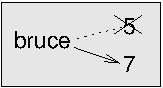
\includegraphics[scale=0.8]{figs/assign2.pdf}}
\caption{Diagramma di stato.}
\label{fig.assign2}
\end{figure}



\section{Aggiornare le variabili}
\label{update}

\index{aggiornamento}
\index{variabile!aggiornamento}

Una delle forme più comuni di riassegnazione è l'{\bf aggiornamento},
dove il nuovo valore della variabile dipende da quello precedente.

\begin{verbatim}
>>> x = x + 1
\end{verbatim}
%
Questo significa: ``prendi il valore attuale di {\tt x}, aggiungi uno, e aggiorna {\tt x} al nuovo valore.''

Se tentate di aggiornare una variabile inesistente, si verifica un errore perché Python valuta il lato destro prima di assegnare un valore a {\tt x}:

\begin{verbatim}
>>> x = x + 1
NameError: name 'x' is not defined
\end{verbatim}
%
Prima di aggiornare una variabile occorre quindi {\bf inizializzarla},
di solito con una comune assegnazione:
\index{inizializzazione!prima di aggiornare}

\begin{verbatim}
>>> x = 0
>>> x = x + 1
\end{verbatim}
%
L'aggiornamento di una variabile aggiungendo 1 è detto {\bf incremento};
sottrarre 1 è detto invece {\bf decremento}.
\index{incremento}
\index{decremento}


\section{L'istruzione {\tt while}}
\index{istruzione!while}
\index{ciclo!while}
\index{iterazione}

Spesso i computer sono usati per automatizzare dei compiti ripetitivi: ripetere operazioni identiche o simili senza fare errori, è qualcosa che i computer fanno molto bene e le persone piuttosto male. Nella programmazione, la ripetizione è chiamata anche {\bf iterazione}.

Abbiamo già visto due funzioni, {\tt contoallarovescia} e \verb"stampa_n", che iterano usando la ricorsione. Dato che l'iterazione è un'operazione molto frequente, Python fornisce varie caratteristiche del linguaggio per renderla più semplice da implementare. Una è l'istruzione {\tt for}, che abbiamo già visto nel Paragrafo~\ref{repetition} e sulla quale torneremo.

Un'altra istruzione è {\tt while}. Ecco una variante di {\tt
contoallarovescia} che usa l'istruzione {\tt while}:

\begin{verbatim}
def contoallarovescia(n):
    while n > 0:
        print(n)
        n = n-1
    print('Via!')
\end{verbatim}
%
Si può quasi leggere il programma con l'istruzione {\tt while} come fosse scritto in inglese: significa ``Finché (while) {\tt n} è maggiore di 0, stampa il valore di {\tt n} e poi decrementa {\tt n} di 1.  Quando arrivi a 0, stampa la stringa {\tt Via!}''
\index{flusso di esecuzione}

In modo più formale, questo è il flusso di esecuzione di un'istruzione {\tt while}:

\begin{enumerate}

\item Determina se la condizione è vera ({\tt True}) o falsa ({\tt False}).

\item Se la condizione è falsa, esce dal ciclo {\tt while} e continua l'esecuzione dalla prima istruzione successiva.

\item Se la condizione è vera, esegue il blocco di istruzioni nel corpo del ciclo while e vi rimane, ritornando al punto 1.

\end{enumerate}

Questo tipo di flusso è chiamato ciclo, (in inglese {\em loop}), perché il terzo punto ritorna ciclicamente da capo. 
\index{condizione}
\index{ciclo}
\index{corpo}

Il corpo del ciclo deve cambiare il valore di una o più variabili in modo che la condizione prima o poi diventi falsa e il ciclo abbia termine. Altrimenti, il ciclo verrebbe ripetuto continuamente, dando luogo ad un {\bf ciclo infinito}. Una fonte inesauribile di divertimento per gli informatici, è osservare che le istruzioni dello shampoo:
``lava, risciacqua, ripeti'' sono un ciclo infinito.

\index{ciclo!infinito}

Nel caso di {\tt contoallarovescia}, è evidente che il ciclo terminerà: se {\tt n} è zero o negativo, il ciclo non viene mai eseguito. Altrimenti, {\tt n} diventa via via più piccolo ad ogni ripetizione del ciclo stesso, fino a diventare, prima o poi, zero. 

In altri cicli, può non essere così evidente. Per esempio:

\begin{verbatim}
def sequenza(n):
    while n != 1:
        print(n)
        if n % 2 == 0:        # n è pari
            n = n / 2
        else:               # n è dispari
            n = n*3+1
\end{verbatim}
%
La condizione di questo ciclo è {\tt n != 1}, per cui il ciclo si ripeterà
fino a quando {\tt n} non sarà uguale a {\tt 1}, cosa che rende falsa la condizione.

Ad ogni ripetizione del ciclo, il programma stampa il valore di {\tt n} e poi controlla se è pari o dispari. Se è pari, {\tt n} viene diviso per 2. Se è dispari, {\tt n} è moltiplicato per 3 e al risultato viene aggiunto 1. Se per esempio il valore passato a {\tt sequenza} è 3, i valori risultanti di {\tt n} saranno nell'ordine 3, 10, 5, 16, 8, 4, 2, 1.

Dato che {\tt n} a volte sale e a volte scende, non c'è modo di stabilire che {\tt n} raggiungerà 1 in modo da terminare il ciclo. Solo per qualche particolare valore di {\tt n}, possiamo dimostrarlo: ad esempio, se il valore di partenza è una potenza di 2, {\tt n} sarà per forza un numero pari ad ogni ciclo, fino a raggiungere 1. L'esempio precedente finisce proprio con una sequenza simile, a partire dal numero 16.
\index{congettura di Collatz}

La domanda difficile è se il programma giunga a termine per {\em qualsiasi} valore positivo di {\tt n}. Sinora, nessuno è riuscito a dimostrarlo {\em né} a smentirlo!  (Vedere \url{http://it.wikipedia.org/wiki/Congettura_di_Collatz}.)

Come esercizio, riscrivete la funzione \verb"stampa_n" del Paragrafo~\ref{recursion} usando l'iterazione al posto della ricorsione.




\section{{\tt break}}
\index{break, istruzione}
\index{istruzione!break}

Vi può capitare di poter stabilire il momento in cui è necessario terminare un ciclo solo mentre il flusso di esecuzione si trova nel bel mezzo del corpo. In questi casi potete usare l'istruzione {\tt break} per interrompere il ciclo e saltarne fuori.

Per esempio, supponiamo che vogliate ricevere delle risposte dall'utente, fino a quando non viene digitata la parola {\tt fine}.  Potete scrivere:

\begin{verbatim}
while True:
    riga = input('> ')
    if riga == 'fine':
        break
    print(riga)

print('Finito!')
\end{verbatim}
%
La condizione del ciclo è {\tt True}, che è sempre vera per definizione, quindi il ciclo è destinato a continuare, a meno che non incontri l'istruzione {\tt break}.

Ad ogni ripetizione, il programma mostra come prompt il simbolo {\tt >}.
Se l'utente scrive {\tt fine}, l'istruzione {\tt break} interrompe il ciclo, altrimenti il programma ripete quello che l'utente ha scritto e ritorna da capo. Ecco un esempio di esecuzione:

\begin{verbatim}
> non ho finito
non ho finito
> fine
Finito!
\end{verbatim}
%
Questo modo di scrivere i cicli {\tt while} è frequente, perché vi permette di controllare la condizione ovunque all'interno del ciclo (e non solo all'inizio) e di esprimere la condizione di stop in modo affermativo (``fermati quando succede questo'') piuttosto che negativo (``continua fino a quando non succede questo'').


\section{Radici quadrate}
\label{squareroot}
\index{radice quadrata}

I cicli si usano spesso per calcolare risultati numerici, partendo da un valore approssimativo che viene migliorato iterativamente con approssimazioni successive.
\index{metodo di Newton}

Per esempio, un modo di calcolare le radici quadrate è il metodo di Newton. Supponiamo di voler calcolare la radice quadrata di $a$. A partire da una qualunque stima, $x$, possiamo calcolare una stima migliore con la formula seguente:

\[ y = \frac{x + a/x}{2} \]
%
Supponiamo per esempio che $a$ sia 4 e $x$ sia 3:

\begin{verbatim}
>>> a = 4
>>> x = 3
>>> y = (x + a/x) / 2
>>> y
2.16666666667
\end{verbatim}
%
Il risultato è più vicino al valore vero ($\sqrt{4} = 2$).  Se ripetiamo il procedimento usando la nuova stima, ci avviciniamo ulteriormente:

\begin{verbatim}
>>> x = y
>>> y = (x + a/x) / 2
>>> y
2.00641025641
\end{verbatim}
%
Dopo qualche ulteriore passaggio, la stima diventa quasi esatta:
\index{aggiornamento}

\begin{verbatim}
>>> x = y
>>> y = (x + a/x) / 2
>>> y
2.00001024003
>>> x = y
>>> y = (x + a/x) / 2
>>> y
2.00000000003
\end{verbatim}
%
In generale, non possiamo sapere {\em a priori} quanti passaggi ci vorranno per ottenere la risposta esatta, ma sapremo che ci saremo arrivati quando la stima non cambierà più:

\begin{verbatim}
>>> x = y
>>> y = (x + a/x) / 2
>>> y
2.0
>>> x = y
>>> y = (x + a/x) / 2
>>> y
2.0
\end{verbatim}
%
Possiamo fermarci quando {\tt y == x}.  Ecco quindi un ciclo che parte da una stima iniziale, {\tt x}, e la migliora fino a quando non cambia più:

\begin{verbatim}
while True:
    print(x)
    y = (x + a/x) / 2
    if y == x:
        break
    x = y
\end{verbatim}
%
Per la maggior parte dei valori di {\tt a}, questo codice funziona bene, ma in genere è pericoloso testare l'uguaglianza su valori decimali di tipo {\tt float},
perché sono solo approssimativamente esatti: la maggior parte dei numeri razionali come $1/3$, e irrazionali, come $\sqrt{2}$, non possono essere rappresentati in modo preciso con un {\tt float}.
\index{virgola mobile}
\index{epsilon}

Piuttosto di controllare se {\tt x} e {\tt y} sono identici, è meglio usare la funzione predefinita {\tt abs} per calcolare il valore assoluto della loro differenza:

\begin{verbatim}
    if abs(y-x) < epsilon:
        break
\end{verbatim}
%
Dove \verb"epsilon" è un valore molto piccolo, come {\tt 0.0000001}, che determina quando i due numeri confrontati sono abbastanza vicini da poter essere considerati praticamente uguali.


\section{Algoritmi}
\index{algoritmo}

Il metodo di Newton è un esempio di {\bf algoritmo}: è un'operazione meccanica per risolvere un tipo di problema (in questo caso, calcolare la radice quadrata).

Per capire cosa sia un algoritmo, può essere utile iniziare a vedere cosa non è un algoritmo. Quando a scuola vi insegnarono a fare le moltiplicazioni dei numeri a una cifra, probabilmente avevate imparato a memoria le tabelline, che significa ricordare 100 specifiche soluzioni. Una conoscenza di questo tipo non è algoritmica.

Ma se eravate dei bambini un po' pigri, probabilmente avevate imparato qualche trucchetto. Per esempio, per trovare il prodotto tra $n$ e 9, si scrive $n-1$ come prima cifra e $10-n$ come seconda cifra. Questo trucco è una soluzione generica per moltiplicare per nove qualunque numero a una cifra. Questo è un algoritmo!
\index{addizione!con riporto}
\index{sottrazione!con prestito}

Similmente, le tecniche che avete imparato per l'addizione con riporto, la sottrazione con prestito e le divisioni lunghe sono tutte algoritmi. Una caratteristica degli algoritmi è che non richiedono intelligenza per essere eseguiti. Sono procedimenti meccanici in cui ad ogni passo ne segue un altro, secondo delle semplici regole.

L'esecuzione di un algoritmo, in sé, è una cosa noiosa e ripetitiva. D'altra parte, la procedura di realizzazione di un algoritmo è interessante, intellettualmente stimolante, e una parte cruciale di quella che chiamiamo programmazione.

Alcune delle cose che le persone fanno in modo naturale senza difficoltà o senza nemmeno pensarci, sono le più difficili da esprimere con algoritmi. Capire il linguaggio naturale è un esempio calzante. Lo facciamo tutti, ma finora nessuno è stato in grado di spiegare {\em come} lo facciamo, almeno non sotto forma di un algoritmo.


\section{Debug}
\label{bisectbug}

Quando inizierete a scrivere programmi di grandi dimensioni, impiegherete più tempo per il debug: più codice significa più probabilità di commettere un errore e più posti in cui gli errori possono annidarsi.
\index{debug!binario}

Un metodo per ridurre il tempo di debug è il ``debug binario''.
Se nel vostro programma ci sono 100 righe e le controllate una ad una, ci vorranno 100 passaggi.

Provate invece a dividere il problema in due. Cercate verso la metà del programma un valore intermedio che potete controllare. Aggiungete un'istruzione di stampa (o qualcos'altro di controllabile) ed eseguite il programma.

Se il controllo nel punto mediano non è corretto, deve esserci un problema nella prima metà del programma. Se invece è corretto, l'errore sarà nella seconda metà.

Per ogni controllo eseguito in questa maniera, dimezzate le righe da controllare. Dopo 6 passaggi (che sono meno di 100), dovreste teoricamente arrivare a una o due righe di codice.

In pratica, non è sempre chiaro quale sia la ``metà del programma'' e non è sempre possibile controllare. Non ha neanche molto senso contare le righe e trovare la metà esatta. Meglio considerare i punti del programma dove è più probabile che vi siano errori e quelli dove è facile posizionare dei controlli. Poi, scegliere un punto dove stimate che le probabilità che l'errore sia prima o dopo quel punto siano circa le stesse.


\section{Glossario}

\begin{description}

\item[riassegnazione:] Assegnazione di un nuovo valore ad una variabile che  esiste già.
\index{riassegnazione}

\item[aggiornamento:] Riassegnazione in cui il nuovo valore della variabile dipende da quello precedente.
\index{aggiornamento}

\item[inizializzazione:] Assegnazione che fornisce un valore iniziale ad una variabile da aggiornare successivamente.
\index{inizializzazione!variabile}

\item[incremento:] Aggiornamento che aumenta il valore di una variabile (spesso di una unità).
\index{incremento}

\item[decremento:] Aggiornamento che riduce il valore di una variabile.
\index{decremento}

\item[iterazione:] Ripetizione di una serie di istruzioni utilizzando una funzione ricorsiva oppure un ciclo.
\index{iterazione}

\item[ciclo infinito:] Ciclo in cui la condizione che ne determina la fine non è mai soddisfatta.
\index{ciclo!infinito}

\item[algoritmo:]  Una procedura generica per risolvere una categoria di problemi.
\index{algoritmo}

\end{description}


\section{Esercizi}

\begin{exercise}
\index{algoritmo!radice quadrata}

Copiate il ciclo del Paragrafo~\ref{squareroot} e incapsulatelo in una funzione
di nome \verb"mia_radq" che prenda {\tt a} come parametro, scelga un valore appropriato di {\tt x}, e restituisca una stima del valore della radice quadrata di {\tt a}.  \index{incapsulamento}

Quale verifica, scrivete una funzione di nome \verb"test_radq" che stampi una tabella come questa:

\begin{verbatim}
a   mia_radq(a)   math.sqrt(a)  diff
-   ----------    ------------  ----
1.0 1.0           1.0           0.0
2.0 1.41421356237 1.41421356237 2.22044604925e-16
3.0 1.73205080757 1.73205080757 0.0
4.0 2.0           2.0           0.0
5.0 2.2360679775  2.2360679775  0.0
6.0 2.44948974278 2.44948974278 0.0
7.0 2.64575131106 2.64575131106 0.0
8.0 2.82842712475 2.82842712475 4.4408920985e-16
9.0 3.0           3.0           0.0
\end{verbatim}
%
La prima colonna è un numero, $a$; la seconda è la radice quadrata di $a$ calcolata con \verb"mia_radq"; la terza è la radice quadrata calcolata con {\tt math.sqrt}; la quarta è il valore assoluto della differenza tra le due stime.
\end{exercise}

\vspace{0.2in}
\begin{exercise}
\index{eval, funzione}
\index{funzione!eval}

La funzione predefinita {\tt eval} valuta un'espressione sotto forma di stringa, usando l'interprete Python. Ad esempio:

\begin{verbatim}
>>> eval('1 + 2 * 3')
7
>>> import math
>>> eval('math.sqrt(5)')
2.2360679774997898
>>> eval('type(math.pi)')
<class 'float'>
\end{verbatim}
%
Scrivete una funzione di nome \verb"eval_ciclo" che chieda iterativamente all'utente di inserire un dato, prenda il dato inserito e lo valuti con {\tt eval}, infine visualizzi il risultato.

Deve continuare fino a quando l'utente non scrive \verb"'fatto'", e poi restituire il valore dell'ultima espressione che ha valutato.

\end{exercise}

\vspace{0.2in}
\begin{exercise}
\index{Ramanujan, Srinivasa}

Il matematico Srinivasa Ramanujan scoprì una serie infinita che può essere usata per generare un'approssimazione di $1 / \pi$:
\index{pi}

\[ \frac{1}{\pi} = \frac{2\sqrt{2}}{9801} 
\sum^\infty_{k=0} \frac{(4k)!(1103+26390k)}{(k!)^4 396^{4k}} \]

Scrivete una funzione di nome \verb"stima_pi" che utilizzi questa formula per calcolare e restituire una stima di $\pi$.  Deve usare un ciclo {\tt while}
per calcolare gli elementi della sommatoria, fino a quando l'ultimo termine è più piccolo di {\tt 1e-15} (che è la notazione di Python per $10^{-15}$).
Controllate il risultato confrontandolo con {\tt math.pi}.

Soluzione: \url{http://thinkpython2.com/code/pi.py}.

\end{exercise}


\chapter{Stringhe}
\label{strings}

Le stringhe non sono valori come gli interi, i float e i booleani. Una stringa è una {\bf sequenza}, vale a dire un insieme ordinato di valori di altra natura.  In questo capitolo vedrete come si accede ai caratteri che compongono una stringa e imparerete alcuni metodi che le stringhe espongono.
\index{sequenza}


\section{Una stringa è una sequenza}
\index{carattere}
\index{parentesi quadre, operatore}
\index{operatore!parentesi quadre}

Una stringa è una sequenza di caratteri. Potete accedere ai singoli caratteri usando gli operatori parentesi quadre:

\begin{verbatim}
>>> frutto = 'banana'
>>> lettera = frutto[1]
\end{verbatim}
%
La seconda istruzione seleziona il carattere numero 1 della variabile {\tt
frutto} e lo assegna alla variabile {\tt lettera}.  
\index{indice}

L'espressione all'interno delle parentesi quadre è chiamato {\bf indice}.  
L'indice è un numero intero che indica (di qui il nome) il carattere della sequenza che desiderate estrarre.

Ma il risultato potrebbe lasciarvi perplessi:

\begin{verbatim}
>>> lettera
a
\end{verbatim}
%
Per la maggior parte delle persone, la prima lettera di \verb"'banana'" è {\tt b}, non
{\tt a}.  Ma per gli informatici, premesso che l'indice è la posizione a partire dall'inizio della stringa, la posizione della prima lettera è considerata la numero zero, non uno.

\begin{verbatim}
>>> lettera = frutto[0]
>>> lettera
b
\end{verbatim}
%
Quindi {\tt b} è la ``zero-esima'' lettera di \verb"'banana'", {\tt a}
è la prima lettera (``1-esima''), e {\tt n} è la seconda (``2-esima'')
lettera.
\index{indice!inizio da zero}
\index{zero, indice iniziale}

Potete usare come indice qualsiasi espressione, compresi variabili e operatori:

\begin{verbatim}
>>> i = 1
>>> frutto[i]
'a'
>>> frutto[i+1]
'n'
\end{verbatim}
%

Tuttavia, il valore risultante deve essere un intero. Altrimenti succede questo:
\index{indice}
\index{eccezione!TypeError}
\index{TypeError}

\begin{verbatim}
>>> lettera = frutto[1.5]
TypeError: string indices must be integers
\end{verbatim}
%

\section{{\tt len}}
\index{len, funzione}
\index{funzione!len}

{\tt len} è una funzione predefinita che restituisce il numero di caratteri contenuti in una stringa:

\begin{verbatim}
>>> frutto = 'banana'
>>> len(frutto)
6
\end{verbatim}
%
Per estrarre l'ultimo carattere di una stringa, si potrebbe pensare di scrivere qualcosa del genere:
\index{eccezione!IndexError}
\index{IndexError}

\begin{verbatim}
>>> lunghezza = len(frutto)
>>> ultimo = frutto[lunghezza]
IndexError: string index out of range
\end{verbatim}
%
La ragione dell'{\tt IndexError} è che non c'è nessuna lettera in {\tt
'banana'} con indice 6. Siccome partiamo a contare da zero, le sei lettere sono numerate da 0 a 5. Per estrarre l'ultimo carattere, dobbiamo perciò sottrarre 1 da {\tt lunghezza}:

\begin{verbatim}
>>> ultimo = frutto[lunghezza-1]
>>> ultimo
'a'
\end{verbatim}
%
Oppure, possiamo usare utilmente gli indici negativi, che contano a ritroso dalla fine della stringa: l'espressione {\tt frutto[-1]} ricava l'ultimo carattere della stringa, {\tt frutto[-2]} il penultimo carattere, e così via.
\index{indice!negativo}


\section{Attraversamento con un ciclo {\tt for}}
\label{for}
\index{attraversamento}
\index{ciclo!attraversamento}
\index{for, ciclo}
\index{ciclo!for}
\index{istruzione!for}

Parecchi tipi di calcolo comportano l'elaborazione di una stringa, un carattere per volta. Spesso iniziano dal primo carattere, selezionano un carattere per volta, eseguono una certa operazione e continuano fino alla fine della stringa. Questo tipo di elaborazione è detta {\bf attraversamento}. Un modo per scrivere un attraversamento è quello di usare un ciclo {\tt while}:

\begin{verbatim}
indice = 0
while indice < len(frutto):
    lettera = frutto[indice]
    print(lettera)
    indice = indice + 1
\end{verbatim}
%
Questo ciclo attraversa tutta la stringa e ne mostra le singole lettere, ciascuna su una riga separata. La condizione del ciclo è {\tt indice < len(frutto)}, per cui quando {\tt indice} è uguale alla lunghezza della stringa, la condizione diventa falsa e il corpo del ciclo non viene più eseguito. L'ultimo carattere a cui si accede è quello di indice {\tt len(frutto)-1}, cioè l'ultimo carattere della stringa.

Come esercizio, scrivete una funzione che riceva una stringa come argomento e ne stampi i singoli caratteri, uno per riga, partendo dall'ultimo a ritroso.

Un altro modo di scrivere un attraversamento è usare un ciclo {\tt for}:

\begin{verbatim}
for lettera in frutto:
    print(lettera)
\end{verbatim}
%
Ad ogni ciclo, il successivo carattere della stringa viene assegnato alla variabile {\tt lettera}. Il ciclo continua finché non rimangono più caratteri da analizzare.
\index{concatenamento}
\index{alfabetico}
\index{McCloskey, Robert}

L'esempio che segue illustra come usare il concatenamento (addizione di stringhe) e un ciclo {\tt for} per generare una serie alfabetica (cioè, disposta in ordine alfabetico). Nel libro {\em Make Way for Ducklings} di Robert McCloskey, ci sono degli anatroccoli che si chiamano Jack, Kack, Lack, Mack, Nack, Ouack, Pack, e Quack.  Questo ciclo restituisce i nomi in ordine:

\begin{verbatim}
prefissi = 'JKLMNOPQ'
suffisso = 'ack'

for lettera in prefissi:
    print(lettera + suffisso)
\end{verbatim}
%
Il risultato del programma è:

\begin{verbatim}
Jack
Kack
Lack
Mack
Nack
Oack
Pack
Qack
\end{verbatim}
%
È evidente che non è del tutto giusto, dato che ``Ouack'' e ``Quack'' sono scritti in modo errato.

Provate a modificare il programma per correggere questo errore.


\section{Slicing}
\label{slice}
\index{slicing!operatore di}
\index{operatore!di slicing}
\index{indice!slicing}
\index{stringa!slicing}
\index{slicing!stringa}

Un segmento o porzione di stringa è chiamato {\bf slice}. L'operazione di selezione di una porzione di stringa è simile alla selezione di un carattere, ed è detta {\bf slicing}:

\begin{verbatim}
>>> s = 'Monty Python'
>>> s[0:5]
'Monty'
>>> s[6:12]
'Python'
\end{verbatim}
%
L'operatore {\tt [n:m]} restituisce la porzione di stringa nell'intervallo compreso tra l'``n-esimo'' carattere incluso fino all'``m-esimo'' escluso. Questo comportamento è poco intuitivo, e per tenerlo a mente può essere d'aiuto immaginare gli indici puntare {\em tra} i caratteri, come spiegato nella Figura~\ref{fig.banana}.

\begin{figure}
\centerline
{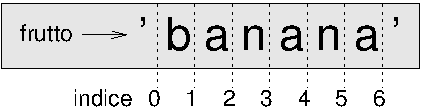
\includegraphics[scale=0.8]{figs/banana.pdf}}
\caption{Indici di slicing.}
\label{fig.banana}
\end{figure}


Se non è specificato il primo indice (quello prima dei due punti :), la porzione parte dall'inizio della stringa. Se manca il secondo indice, la porzione arriva fino in fondo alla stringa:

\begin{verbatim}
>>> frutto = 'banana'
>>> frutto[:3]
'ban'
>>> frutto[3:]
'ana'
\end{verbatim}
%
Se il primo indice è maggiore o uguale al secondo, il risultato è una {\bf stringa vuota}, rappresentata da due apici consecutivi.
\index{apici}

\begin{verbatim}
>>> frutto = 'banana'
>>> frutto[3:3]
''
\end{verbatim}
%
Una stringa vuota non contiene caratteri e ha lunghezza 0, ma a parte questo è a tutti gli effetti una stringa come le altre.

Proseguendo con l'esempio, data una stringa di nome {\tt frutto}, secondo voi che cosa significa {\tt frutto[:]}? Provate a vedere.
\index{copia!slicing}
\index{slicing!copia}


\section{Le stringhe sono immutabili}
\index{mutabilità}
\index{immutabilità}
\index{stringa!immutabile}

Per sostituire un carattere all'interno di una stringa, potreste pensare di utilizzare l'operatore {\tt []} sul lato sinistro di un'assegnazione, per esempio così:
\index{TypeError}
\index{eccezione!TypeError}

\begin{verbatim}
>>> saluto = 'Ciao, mondo!'
>>> saluto[0] = 'M'
TypeError: 'str' object does not support item assignment
\end{verbatim}
%
L'``oggetto'' ({\em object}) in questo caso è la stringa, e l'``elemento'' ({\em item}) è il carattere che avete tentato di assegnare. Per ora, consideriamo un  oggetto come la stessa cosa di un valore, ma più avanti (Paragrafo~\ref{equivalence}) puntualizzeremo meglio questa definizione. 
\index{oggetto}
\index{elemento}
\index{elemento!assegnazione}
\index{assegnazione!elemento}
\index{immutabilità}

La ragione dell'errore è che le stringhe sono {\bf immutabili}, in altre parole, non è consentito cambiare una stringa esistente. La cosa migliore da fare è creare una nuova stringa, variante dell'originale:

\begin{verbatim}
>>> saluto = 'Ciao, mondo!'
>>> nuovo_saluto = 'M' + saluto[1:]
>>> nuovo_saluto
'Miao, mondo!'
\end{verbatim}
%
Questo esempio concatena una nuova prima lettera con la restante porzione di {\tt saluto}. Non ha alcun effetto sulla stringa di origine, che resta invariata.
\index{concatenamento}


\section{Ricerca}
\label{find}

Cosa fa la funzione seguente?
\index{trova, funzione}
\index{funzione!trova}

\begin{verbatim}
def trova(parola, lettera):
    indice = 0
    while indice < len(parola):
        if parola[indice] == lettera:
            return indice
        indice = indice + 1
    return -1
\end{verbatim}
%
In un certo senso, {\tt trova} è l'inverso dell'operatore {\tt []}.
Anziché prendere un indice ed estrarre il carattere corrispondente, prende un carattere e trova l'indice in corrispondenza del quale appare il carattere. Se non trova il carattere indicato nella parola data, la funzione restituisce {\tt -1}.

Per la prima volta incontriamo l'istruzione {\tt return} all'interno di un ciclo. Se {\tt parola[indice] == lettera}, la funzione interrompe il ciclo e ritorna immediatamente, restituendo {\tt indice}. 

Se il carattere non compare nella stringa data, il programma termina il ciclo  normalmente e restituisce {\tt -1}.

Questo schema di calcolo---attraversare una sequenza e ritornare quando si trova ciò che si sta cercando---è chiamato {\bf ricerca}.
\index{attraversamento}
\index{ricerca!schema di}
\index{schema!di ricerca}

Come esercizio, modificate la funzione {\tt trova} in modo che richieda un terzo parametro, che rappresenta la posizione da cui si deve cominciare la ricerca all'interno della stringa {\tt parola}.


\section{Cicli e contatori}
\label{counter}
\index{contatore}
\index{contatori e cicli}
\index{cicli e contatori}
\index{ciclo!con stringhe}

Il programma seguente conta il numero di volte in cui la lettera {\tt a}
compare in una stringa:

\begin{verbatim}
parola = 'banana'
conta = 0
for lettera in parola:
    if lettera == 'a':
        conta = conta + 1
print(conta)
\end{verbatim}
%
Si tratta di un altro schema di calcolo chiamato {\bf contatore}.  La variabile {\tt conta} è inizializzata a 0, quindi incrementata di uno per ogni volta che viene trovata una {\tt a}.
Al termine del ciclo, {\tt conta} contiene il risultato: il numero totale di lettere {\tt a} nella stringa.

Come esercizio, incapsulate questo codice in una funzione di nome {\tt conta}, e generalizzatela in modo che accetti come argomenti sia la stringa che la lettera da cercare.
Quindi, riscrivete questa funzione in modo che, invece di attraversare completamente la stringa, faccia uso della versione a tre parametri di {\tt trova}, vista nel precedente paragrafo.
\index{incapsulamento}

\section{Metodi delle stringhe}
\label{optional}

Le stringhe espongono dei metodi che permettono di effettuare molte utili operazioni. Un {\bf metodo} è simile a una funzione---riceve argomenti e restituisce un valore---ma la sintassi è diversa. Prendiamo ad esempio il metodo {\tt upper}, che prende una stringa e crea una nuova stringa di tutte lettere maiuscole.
\index{metodo}
\index{stringa!metodi}

Al posto della sintassi delle funzioni, {\tt upper(parola)}, si usa la sintassi dei metodi, {\tt parola.upper()}.

\begin{verbatim}
>>> parola = 'banana'
>>> nuova_parola = parola.upper()
>>> nuova_parola
BANANA
\end{verbatim}
%
Questa forma di notazione a punto, in inglese {\em dot notation}, specifica il nome del metodo, {\tt upper}, preceduto dal nome della stringa a cui va applicato il metodo, {\tt parola}. Le parentesi vuote indicano che il metodo non ha argomenti.
\index{parentesi!vuote}
\index{notazione a punto}

La chiamata di un metodo è detta {\bf invocazione}; nel nostro caso, diciamo che stiamo invocando {\tt upper} su {\tt parola}.
\index{invocazione}

Visto che ci siamo, esiste un metodo delle stringhe chiamato {\tt find} che è molto simile alla funzione che abbiamo scritto prima:

\begin{verbatim}
>>> parola = 'banana'
>>> indice = parola.find('a')
>>> indice
1
\end{verbatim}
%
In questo esempio, abbiamo invocato {\tt find} su {\tt parola} e abbiamo passato come parametro la lettera che stiamo cercando.

In realtà, il metodo {\tt find} è più generale della nostra funzione: può ricercare anche sottostringhe e non solo singoli caratteri:

\begin{verbatim}
>>> parola.find('na')
2
\end{verbatim}
%
Di default, {\tt find} parte dall'inizio della stringa, ma può ricevere come secondo argomento l'indice da cui partire:
\index{argomento!opzionale}

\begin{verbatim}
>>> parola.find('na', 3)
4
\end{verbatim}
%
Questo è un esempio di {\bf argomento opzionale}; {\tt find} può anche avere un terzo argomento opzionale, l'indice in corrispondenza del quale fermarsi:

\begin{verbatim}
>>> nome = 'bob'
>>> nome.find('b', 1, 2)
-1
\end{verbatim}
%
In quest'ultimo caso la ricerca fallisce, perché {\tt b} non è compreso nell'intervallo da {\tt 1} a {\tt 2}, in quanto {\tt 2} si considera escluso. Questo comportamento rende {\tt find} coerente con l'operatore di slicing.


\section{L'operatore {\tt in}}
\label{inboth}
\index{in, operatore}
\index{operatore!in}
\index{booleano, operatore}
\index{operatore!booleano}

La parola {\tt in} è un operatore booleano che confronta due stringhe e restituisce {\tt True} se la prima è una sottostringa della seconda:

\begin{verbatim}
>>> 'a' in 'banana'
True
>>> 'seme' in 'banana'
False
\end{verbatim}
%
Ad esempio, la funzione che segue stampa tutte le lettere di {\tt parola1} che compaiono anche in {\tt parola2}:

\begin{verbatim}
def in_entrambe(parola1, parola2):
    for lettera in parola1:
        if lettera in parola2:
            print(lettera)
\end{verbatim}
%
Con qualche nome di variabile scelto bene, Python a volte si legge quasi come fosse un misto di inglese e italiano: ``per (ogni) lettera in parola1, se (la) lettera (è) in parola2, stampa (la) lettera.''

Ecco cosa succede se paragonate carote e patate:

\begin{verbatim}
>>> in_entrambe('carote', 'patate')
a
t
e
\end{verbatim}
%

\section{Confronto di stringhe}
\index{stringa!confronto}
\index{confronto!stringa}

Gli operatori di confronto funzionano anche sulle stringhe. Per controllare se
due stringhe sono uguali:

\begin{verbatim}
if parola == 'banana':
    print('Tutto ok, banane.')
\end{verbatim}
%
Altri operatori di confronto sono utili per mettere le parole in ordine alfabetico:

\begin{verbatim}
if parola < 'banana':
    print('La tua parola,' + parola + ', viene prima di banana.')
elif parola > 'banana':
    print('La tua parola,' + parola + ', viene dopo banana.')
else:
    print('Tutto ok, banane.')
\end{verbatim}
%
Attenzione che Python non gestisce le lettere maiuscole e minuscole come siamo abituati: in un confronto, le lettere maiuscole vengono sempre prima di tutte le minuscole, così che:

\begin{verbatim}
La tua parola, Papaya, viene prima di banana.
\end{verbatim}
%
Questo problema si risolve facilmente convertendo le stringhe in un formato standard, ad esempio tutte lettere minuscole, prima di effettuare il confronto.


\section{Debug}
\index{debug}
\index{attraversamento}

Quando usate gli indici per l'attraversamento dei valori di una sequenza, non è facile determinare bene l'inizio e la fine. Ecco una funzione che dovrebbe confrontare due parole e restituire {\tt True} quando una parola è scritta al contrario dell'altra, ma contiene due errori:

\begin{verbatim}
def al_contrario(parola1, parola2):
    if len(parola1) != len(parola2):
        return False
    
    i = 0
    j = len(parola2)

    while j > 0:
        if parola1[i] != parola2[j]:
            return False
        i = i+1
        j = j-1

    return True
\end{verbatim}
%
La prima istruzione {\tt if} controlla se le parole sono della stessa lunghezza. Se non è così, possiamo restituire immediatamente {\tt False}. Altrimenti, per il resto della funzione, possiamo presupporre che le parole abbiano pari lunghezza. È un altro esempio di condizione di guardia, vista nel Paragrafo~\ref{guardian}.
\index{guardia, condizione di}
\index{schema!guardiani}
\index{indice}

{\tt i} e {\tt j} sono indici: {\tt i} attraversa {\tt parola1}
in avanti, mentre {\tt j} attraversa {\tt parola2} a ritroso. Se troviamo due lettere che non coincidono, possiamo restituire subito {\tt False} Se continuiamo per tutto il ciclo e tutte le lettere coincidono, il valore di ritorno è {\tt True}.

Se proviamo la funzione con i valori ``pots'' e ``stop'', ci aspetteremmo di ricevere di ritorno {\tt True}, invece risulta un IndexError:
\index{IndexError}
\index{eccezione!IndexError}

\begin{verbatim}
>>> al_contrario('pots', 'stop')
...
  File "reverse.py", line 15, in al_contrario
    if parola1[i] != parola2[j]:
IndexError: string index out of range
\end{verbatim}
%
Per fare il debug, la mia prima mossa è di stampare il valore degli indici appena prima della riga dove è comparso l'errore.

\begin{verbatim}
    while j > 0:
        print(i, j)       # stampare qui
        
        if parola1[i] != parola2[j]:
            return False
        i = i+1
        j = j-1
\end{verbatim}
%
Ora, eseguendo di nuovo il programma, ho qualche informazione in più:

\begin{verbatim}
>>> al_contrario('pots', 'stop')
0 4
...
IndexError: string index out of range
\end{verbatim}
%
Alla prima esecuzione del ciclo, il valore di {\tt j} è 4,
che è fuori intervallo della stringa \verb"'pots'".
Infatti l'indice dell'ultimo carattere è 3, e il valore iniziale di {\tt j} va corretto in {\tt len(parola2)-1}.

Se correggo l'errore e rieseguo ancora il programma:

\begin{verbatim}
>>> al_contrario('pots', 'stop')
0 3
1 2
2 1
True
\end{verbatim}
%
Stavolta il risultato è giusto, ma pare che il ciclo sia stato eseguito solo per tre volte, il che è sospetto. Per avere un'idea di cosa stia succedendo, è utile disegnare un diagramma di stato. Durante la prima iterazione, il frame di \verb"al_contrario" è illustrato in Figura~\ref{fig.state4}.
\index{diagramma!di stato}

\begin{figure}
\centerline
{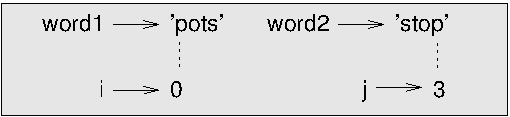
\includegraphics[scale=0.8]{figs/state4.pdf}}
\caption{Diagramma di Stato.}
\label{fig.state4}
\end{figure}

Mi sono preso la libertà di disporre le variabili nel frame e di aggiungere delle linee tratteggiate per evidenziare che i valori di {\tt i} e
{\tt j} indicano i caratteri in {\tt parola1} e {\tt parola2}.

Partendo da questo diagramma, sviluppate il programma su carta cambiando i valori di {\tt i} e {\tt j} ad ogni iterazione. Trovate e correggete il secondo errore in questa funzione.
\label{isreverse}


\section{Glossario}

\begin{description}

\item[oggetto:] Qualcosa a cui una variabile può fare riferimento. Per ora, potete utilizzare ``oggetto'' e ``valore'' indifferentemente.
\index{oggetto}

\item[sequenza:] Una raccolta ordinata di valori, in cui ciascun valore è identificato da un numero intero.
\index{sequenza}

\item[elemento:] Uno dei valori di una sequenza.
\index{elemento}

\item[indice:] Un valore intero usato per selezionare un elemento di una sequenza, come un carattere in una stringa. In Python gli indici partono da 0.
\index{indice}

\item[slice:] Porzione di una stringa identificata tramite un intervallo di indici.
\index{slice}

\item[stringa vuota:] Una stringa priva di caratteri e di lunghezza 0, rappresentata da due apici o virgolette successivi.
\index{stringa!vuota}

\item[immutabile:] Detto di una sequenza i cui elementi non possono essere cambiati.
\index{immutabilità}

\item[attraversare:] Iterare attraverso gli elementi di una sequenza, effettuando su ciascuno un'operazione simile.
\index{attraversamento}

\item[ricerca:] Schema di attraversamento che si ferma quando trova ciò che si sta cercando.
\index{ricerca!schema di}
\index{schema!di ricerca}

\item[contatore:] Variabile utilizzata per contare qualcosa, solitamente inizializzata a zero e poi incrementata.
\index{contatore}

\item[invocazione:] Istruzione che chiama un metodo.
\index{invocazione}

\item[argomento opzionale:] Un argomento di una funzione o di un metodo che non è obbligatorio.
\index{opzionale, argomento}
\index{argomento!opzionale}

\end{description}


\section{Esercizi}

\begin{exercise}
\index{stringa!metodi}
\index{metodo!stringa}

Leggete la documentazione dei metodi delle stringhe sul sito
\url{http://docs.python.org/3/library/stdtypes.html#string-methods}.
Fate degli esperimenti con alcuni metodi per assicurarvi di avere capito come funzionano. {\tt strip} e {\tt replace} sono particolarmente utili.

La documentazione utilizza una sintassi che può risultare poco chiara. Per esempio, in \verb"find(sub[, start[, end]])", le parentesi quadre indicano dei parametri opzionali (non vanno digitate). Quindi {\tt sub} è obbligatorio, ma
{\tt start} è opzionale, e se indicate {\tt start}, allora {\tt end} è a sua volta opzionale.
\index{opzionale, argomento}
\index{argomento!opzionale}

\end{exercise}

\vspace{0.2in}
\begin{exercise}
\index{count, metodo}
\index{metodo!count}

Esiste un metodo delle stringhe di nome {\tt count} che è simile alla funzione del Paragrafo~\ref{counter}.  Leggete la documentazione del metodo e scrivete un'invocazione che conti il numero di {\tt a} in \verb"'banana'".
\end{exercise}

\vspace{0.2in}
\begin{exercise}
\index{step, ampiezza}
\index{slicing!operatore di}
\index{operatore!di slicing}

Nello slicing, si può specificare un terzo indice che stabilisce lo {\em step} o ``passo'', cioè il numero di elementi da saltare tra un carattere estratto e il successivo. Uno step di 2 significa estrarre un carattere ogni 2 (uno sì, uno no), 3 significa uno ogni 3 (uno sì, due no), ecc.

\begin{verbatim}
>>> frutto = 'banana'
>>> frutto[0:5:2]
'bnn'
\end{verbatim}

Uno step di -1 fa scorrere all'indietro nella parola, per cui lo slicing \verb"[::-1]" genera una stringa scritta al contrario.
\index{palindromo}

Usate questo costrutto per scrivere una variante di una sola riga della funzione \verb"palindromo" dell'Esercizio~\ref{palindrome}.
\end{exercise}

\vspace{0.2in}
\begin{exercise}

Tutte le funzioni che seguono {\em dovrebbero} controllare se una stringa contiene almeno una lettera minuscola, ma qualcuna di esse è sbagliata. Per ogni funzione, descrivete cosa fa in realtà (supponendo che il parametro sia una stringa).

\begin{verbatim}
def una_minuscola1(s):
    for c in s:
        if c.islower():
            return True
        else:
            return False

def una_minuscola2(s):
    for c in s:
        if 'c'.islower():
            return 'True'
        else:
            return 'False'

def una_minuscola3(s):
    for c in s:
        flag = c.islower()
    return flag

def una_minuscola4(s):
    flag = False
    for c in s:
        flag = flag or c.islower()
    return flag

def una_minuscola5(s):
    for c in s:
        if not c.islower():
            return False
    return True
\end{verbatim}

\end{exercise}

\vspace{0.2in}
\begin{exercise}
\index{rotazione di lettere}


\label{exrotate}
Un cifrario di Cesare è un metodo di criptazione debole che consiste nel ``ruotare'' ogni lettera di una parola di un dato numero di posti seguendo la sequenza alfabetica, ricominciando da capo quando necessario. Ad esempio 'A' ruotata di 3 posti diventa 'D', 'Z' ruotata di 1 posto diventa 'A'.

Per ruotare una parola, si ruota ciascuna delle sue lettere dello stesso numero di posti prefissato.
Per esempio, ``cheer'' ruotata di 7 dà ``jolly'' e ``melon'' ruotata di -10
dà ``cubed''.  Nel film {\em 2001: Odissea nello Spazio}, il computer di bordo si chiama HAL, che non è altro che IBM ruotato di -1.

Scrivete una funzione di nome \verb"ruota_parola" che richieda una stringa e un intero come parametri, e che restituisca una nuova stringa che contiene le lettere della stringa di partenza ruotate della quantità indicata.

Potete usare le funzioni predefinite {\tt ord}, che converte un carattere in un codice numerico, e {\tt chr}, che converte i codici numerici in caratteri.
Le lettere sono codificate con il loro numero di ordine alfabetico, per esempio:

\begin{verbatim}
>>> ord('c') - ord('a')
2
\end{verbatim}

Dato che \verb"'c'" è la ``2-esima'' lettera dell'alfabeto.  Ma attenzione: i codici numerici delle lettere maiuscole sono diversi.

Su Internet, talvolta, vengono codificate in ROT13 (un cifrario di Cesare con rotazione 13) delle barzellette potenzialmente offensive. Se non siete suscettibili, cercatene qualcuna e decodificatela. Soluzione: \url{http://thinkpython2.com/code/rotate.py}.

\end{exercise}


\chapter{Esercitazione: Giochi con le parole}
\label{wordplay}

Questo capitolo contiene la seconda esercitazione, in cui dovrete risolvere dei quesiti che consistono nel ricercare parole che hanno delle particolari proprietà. Ad esempio, cercherete i più lunghi palindromi della lingua inglese e le parole le cui lettere sono disposte in ordine alfabetico. Illustrerò anche un'altra tecnica di sviluppo: la riduzione ad un problema già risolto.

\section{Leggere elenchi di parole}
\label{wordlist}

Per gli esercizi di questo capitolo ci serve un elenco di parole in inglese. Ci sono parecchi elenchi di parole disponibili sul Web, ma uno dei più adatti ai nostri scopi è quello raccolto da Grady Ward, di pubblico dominio, parte del progetto lessicale Moby (vedere \url{http://wikipedia.org/wiki/Moby_Project}). È un elenco di 113.809 parole ufficiali per cruciverba, cioè parole che sono considerate valide in un gioco di parole crociate o altri giochi con le parole. Nella raccolta Moby il nome del file è {\tt 113809of.fic}; potete anche scaricare una copia chiamata più semplicemente {\tt words.txt}, dal sito
\url{http://thinkpython2.com/code/words.txt}.
\index{Moby Project}
\index{cruciverba}

Il file è in testo semplice, e potete aprirlo con qualsiasi editor di testo, ma anche leggerlo con Python: la funzione predefinita {\tt open} richiede come parametro il nome di un file e restituisce un {\bf oggetto file} che potete utilizzare per questo scopo.
\index{open, funzione}
\index{funzione!open}
\index{testo!semplice}
\index{oggetto!file}

\begin{verbatim}
>>> fin = open('words.txt')
\end{verbatim}
%
{\tt fin} è un nome comunemente usato per un oggetto file usato per operazioni di input.

L'oggetto file comprende alcuni metodi di lettura, come {\tt readline}, che legge i caratteri da un file finché non giunge ad un ritorno a capo, e restituisce il risultato sotto forma di stringa:
\index{readline, metodo}
\index{metodo!readline}

\begin{verbatim}
>>> fin.readline()
'aa\n'
\end{verbatim}
%
La prima parola di questa speciale lista è ``aa'', che è un tipo di lava vulcanica. La sequenza \verb"\n" rappresenta il carattere di ritorno a capo che separa questa parola dalla successiva.

L'oggetto file tiene traccia del punto in cui si trova all'interno del file, così quando chiamate nuovamente {\tt readline}, ottenete la parola successiva:

\begin{verbatim}
>>> fin.readline()
'aah\n'
\end{verbatim}
%
La parola successiva è ``aah'', che è perfettamente valida per cui non fate quella faccia! Oppure, se il carattere di ritorno a capo vi dà fastidio, potete sbarazzarvene con il metodo delle stringhe {\tt strip}:
\index{strip, metodo}
\index{metodo!strip}

\begin{verbatim}
>>> riga = fin.readline()
>>> parola = riga.strip()
>>> parola
'aahed'
\end{verbatim}
%
Potete anche usare un oggetto file all'interno di un ciclo {\tt for}.
Questo programma legge {\tt words.txt} e stampa ogni parola, una per riga:
\index{open, funzione}
\index{funzione!open}

\begin{verbatim}
fin = open('words.txt')
for riga in fin:
    parola = riga.strip()
    print(parola)
\end{verbatim}
%




\section{Esercizi}

Le soluzioni a questi esercizi sono discusse nel prossimo paragrafo. Tentate almeno di risolverli prima di continuare la lettura.

\vspace{0.2in}
\begin{exercise}

Scrivete un programma che legga il file {\tt words.txt} e stampi solo le parole composte da più di 20 caratteri (caratteri spaziatori esclusi).
\index{spaziatore}

\end{exercise}

\vspace{0.2in}
\begin{exercise}

Nel 1939, Ernest Vincent Wright pubblicò una novella di 50.000 parole dal titolo
{\em Gadsby} che non conteneva alcuna lettera ``e''.  Dato che la ``e'' è la lettera più comune nella lingua inglese, non è una cosa facile.

Infatti, in italiano non ho mai composto un piccolo brano siffatto: sono pochi i vocaboli privi tali da riuscirci; finora non ho trovato alcun modo, ma conto di arrivarci in alcuni giorni, pur con un po' di difficoltà! Ma ora, basta così.

Scrivete una funzione di nome \verb"niente_e" che restituisca {\tt True} se una data parola non contiene la lettera ``e''.

Modificate il programma del paragrafo precedente in modo che stampi solo le parole dell'elenco prive della lettera ``e'', e ne calcoli la percentuale sul totale delle parole.
\index{lipogramma}

\end{exercise}

\vspace{0.2in}
\begin{exercise} 

Scrivete una funzione di nome {\tt evita} che richieda una parola e una stringa di lettere vietate, e restituisca {\tt True} se la parola non contiene alcuna lettera vietata.

Modificate poi il programma in modo che chieda all'utente di inserire una stringa di lettere vietate, e poi stampi il numero di parole che non ne contengono alcuna. Riuscite a trovare una combinazione di 5 lettere vietate che escluda il più piccolo numero di parole?

\end{exercise}


\vspace{0.2in}
\begin{exercise}

Scrivete una funzione di nome \verb"usa_solo" che richieda una parola e una stringa di lettere, e che restituisca {\tt True} se la parola contiene solo le lettere indicate. Riuscite a comporre una frase in inglese usando solo le lettere
{\tt acefhlo}?  Diversa da ``Hoe alfalfa''?

\end{exercise}

\vspace{0.2in}
\begin{exercise} 

Scrivete una funzione di nome \verb"usa_tutte" che richieda una parola e una stringa di lettere richieste e che restituisca {\tt True} se la parola utilizza tutte le lettere richieste almeno una volta. Quante parole ci sono che usano tutte le vocali {\tt aeiou}?  E {\tt aeiouy}?

\end{exercise}

\vspace{0.2in}
\begin{exercise}

Scrivete una funzione di nome \verb"alfabetica" che restituisca 
{\tt True} se le lettere di una parola compaiono in ordine alfabetico (le doppie valgono). Quante parole ``alfabetiche'' ci sono?
\index{alfabetico}

\end{exercise}


\section{Ricerca}
\label{search}
\index{ricerca!schema di}
\index{schema!di ricerca}

Tutti gli esercizi del paragrafo precedente hanno qualcosa in comune: possono essere risolti con lo schema di ricerca che abbiamo visto nel Paragrafo~\ref{find}.  L'esempio più semplice è:

\begin{verbatim}
def niente_e(parola):
    for lettera in parola:
        if lettera == 'e':
            return False
    return True
\end{verbatim}
%
Il ciclo {\tt for} attraversa i caratteri in {\tt parola}.  Se trova la lettera  ``e'', può immediatamente restituire {\tt False}; altrimenti deve esaminare la lettera seguente. Se il ciclo termina normalmente, vuol dire che non è stata trovata alcuna ``e'', per cui il risultato è {\tt True}.
\index{attraversamento}
\index{in, operatore}
\index{operatore!in}

Si potrebbe scrivere questa funzione in modo più conciso usando l'operatore {\tt in}, ma ho preferito iniziare con questa versione perché dimostra la logica dello schema di ricerca.
\index{generalizzazione}

{\tt evita} è una versione più generale di \verb"niente_e", ma la struttura è la stessa:

\begin{verbatim}
def evita(parola, vietate):
    for lettera in parola:
        if lettera in vietate:
            return False
    return True
\end{verbatim}
%
Possiamo restituire {\tt False} appena troviamo una delle lettere vietate; se arriviamo alla fine del ciclo, viene restituito {\tt True}.

\verb"usa_solo" è simile, solo che il senso della condizione è invertito:

\begin{verbatim}
def usa_solo(parola, valide):
    for lettera in parola: 
        if lettera not in valide:
            return False
    return True
\end{verbatim}
%
Invece di un elenco di lettere vietate, ne abbiamo uno di lettere disponibili. Se in {\tt parola} troviamo una lettera che non è una di quelle {\tt valide}, possiamo restituire {\tt False}.

\verb"usa_tutte" è ancora simile, solo che rovesciamo il ruolo della parola e della stringa di lettere:

\begin{verbatim}
def usa_tutte(parola, richieste):
    for lettera in richieste: 
        if lettera not in parola:
            return False
    return True
\end{verbatim}
%
Invece di attraversare le lettere in {\tt parola}, il ciclo attraversa le lettere richieste. Se una qualsiasi delle lettere richieste non compare nella parola, restituiamo {\tt False}.
\index{attraversamento}

Ma se avete pensato davvero da informatici, avrete riconosciuto che \verb"usa_tutte" era un'istanza di un problema già risolto in precedenza, e avrete scritto:

\begin{verbatim}
def usa_tutte(parola, richieste):
    return usa_solo(richieste, parola)
\end{verbatim}
%
Ecco un esempio di metodo di sviluppo di un programma chiamato {\bf riduzione ad un problema già risolto}, che significa che avete riconosciuto che il problema su cui state lavorando è un'istanza di un problema già risolto in precedenza, al quale potete applicare una soluzione che avevate già sviluppato.
\index{riduzione ad un problema già risolto}
\index{tecnica di sviluppo!riduzione}


\section{Cicli con gli indici}
\index{ciclo!con indici}
\index{indice!nei cicli}

Ho scritto le funzioni del paragrafo precedente utilizzando dei cicli {\tt for}
perché avevo bisogno solo dei caratteri nelle stringhe e non dovevo fare nulla con gli indici.

Per \verb"alfabetica" dobbiamo comparare delle lettere adiacenti, che è un po' laborioso con un ciclo {\tt for}:

\begin{verbatim}
def alfabetica(parola):
    precedente = parola[0]
    for c in parola:
        if c < precedente:
            return False
        precedente = c
    return True
\end{verbatim}


Un'alternativa è usare la ricorsione:

\begin{verbatim}
def alfabetica(parola):
    if len(parola) <= 1:
        return True
    if parola[0] > parola[1]:
        return False
    return alfabetica(parola[1:])
\end{verbatim}

E un'altra opzione è usare un ciclo {\tt while}:

\begin{verbatim}
def alfabetica(parola):
    i = 0
    while i < len(parola)-1:
        if parola[i+1] < parola[i]:
            return False
        i = i+1
    return True
\end{verbatim}
%
Il ciclo comincia da {\tt i=0} e finisce a {\tt i=len(parola)-1}.  Ogni volta che viene eseguito, il ciclo confronta l' $i$-esimo carattere (consideratelo come il carattere attuale) con l' $i+1$-esimo carattere (consideratelo come quello successivo).

Se il carattere successivo è minore di quello attuale (cioè viene alfabeticamente prima), allora abbiamo scoperto un'interruzione nella serie alfabetica e la funzione restituisce {\tt False}.

Se arriviamo a fine ciclo senza trovare difetti, la parola ha superato il test. Per convincervi che il ciclo è terminato correttamente, prendete un esempio come \verb"'flossy'".  La lunghezza della parola è 6, quindi l'ultima ripetizione del ciclo si ha quando {\tt i} è 4, che è l'indice del penultimo carattere. Nell'ultima iterazione, il penultimo carattere è comparato all'ultimo, che è quello che vogliamo.
\index{palindromo}

Ecco una variante di \verb"palindromo" (vedere l'Esercizio~\ref{palindrome}) che usa due indici; uno parte dall'inizio e aumenta, uno parte dalla fine e diminuisce.

\begin{verbatim}
def palindromo(parola):
    i = 0
    j = len(parola)-1

    while i<j:
        if parola[i] != parola[j]:
            return False
        i = i+1
        j = j-1

    return True
\end{verbatim}

Oppure, possiamo ridurre ad un problema già risolto e scrivere:

\begin{verbatim}
def palindromo(parola):
    return al_contrario(parola, parola)
\end{verbatim}
\index{riduzione ad un problema già risolto}
\index{tecnica di sviluppo!riduzione}

Usando \verb"al_contrario" del Paragrafo~\ref{isreverse}.


\section{Debug}
\index{debug}
\index{test!difficoltà}
\index{programma!test}

Collaudare i programmi non è facile. Le funzioni di questo capitolo sono relativamente agevoli da provare, perché potete facilmente controllare il risultato da voi. Nonostante ciò, scegliere un insieme di parole che riescano a escludere ogni possibile errore è un qualcosa tra il difficile e l'impossibile.

Prendiamo ad esempio \verb"niente_e". Ci sono due evidenti casi da controllare: le parole che hanno una o più 'e' devono dare come risultato {\tt False};
quelle che invece non hanno `e', {\tt True}. E fin qui, in un caso o nell'altro, non c'è niente di particolarmente difficile.

Per ciascun caso ci sono alcuni sottocasi meno ovvi. Tra le parole che contengono ``e'', dovreste provare parole che iniziano con ``e'', finiscono con ``e'', hanno ``e'' da qualche parte nel mezzo della parola. Dovreste poi provare parole lunghe, parole corte e parole cortissime. Nello specifico, la stringa vuota è un esempio di {\bf caso particolare}, che è uno dei casi meno ovvi dove si nascondono spesso gli errori.
\index{caso!particolare}

Oltre che con i casi da voi ideati, sarebbe anche bene fare un test del vostro programma con un elenco di parole come {\tt words.txt}.  Scansionando l'output potreste intercettare qualche errore, ma attenzione: può trattarsi di un certo tipo di errore (parole che non dovrebbero essere incluse ma invece ci sono) e non di un altro (parole che dovrebbero essere incluse ma non ci sono).

In linea generale, fare dei test può aiutarvi a trovare i bug, ma non è facile generare un buon insieme di casi di prova, e anche se ci riuscite non potete essere certi che il vostro programma sia corretto al 100 per cento.

Secondo un leggendario informatico:
\index{test!e assenza di bug}

\begin{quote}
Il test di un programma può essere usato per dimostrare la presenza di bug, ma mai per dimostrarne l'assenza!

--- Edsger W. Dijkstra
\end{quote}
\index{Dijkstra, Edsger}


\section{Glossario}

\begin{description}

\item[oggetto file:] Un valore che rappresenta un file aperto.
\index{oggetto!file}

\item[riduzione ad un problema già risolto:] Modo di risolvere un problema esprimendolo come un'istanza di un problema precedentemente risolto.
\index{riduzione ad un problema già risolto}
\index{tecnica di sviluppo!riduzione}

\item[caso particolare:] un caso atipico o non ovvio (e con meno probabilità di essere gestito correttamente) che viene testato.
\index{caso!particolare}

\end{description}


\section{Esercizi}

\begin{exercise}
\index{Car Talk}
\index{quesito}
\index{lettere!doppie}

Questa domanda deriva da un quesito trasmesso nel programma radiofonico {\em Car Talk} 
(\url{http://www.cartalk.com/content/puzzlers}):

\begin{quote}
``Ditemi una parola inglese con tre lettere doppie consecutive. Vi dò un paio di parole che andrebbero quasi bene, ma non del tutto. Per esempio la parola ``committee'', c-o-m-m-i-t-t-e-e. Sarebbe buona se non fosse per la ``i'' che si insinua in mezzo. O ``Mississippi'': M-i-s-s-i-s-s-i-p-p-i. Togliendo le ``i'' andrebbe bene. Ma esiste una parola che ha tre coppie di lettere uguali consecutive, e per quanto ne so dovrebbe essere l'unica. Magari ce ne sono altre 500, ma me ne viene in mente solo una. Qual è?''
\end{quote}

Scrivete un programma per trovare la parola.  Soluzione: \url{http://thinkpython2.com/code/cartalk1.py}.

\end{exercise}

\vspace{0.2in}
\begin{exercise}
Ecco un altro quesito di {\em Car Talk}
(\url{http://www.cartalk.com/content/puzzlers}):
\index{Car Talk}
\index{Puzzler}
\index{contachilometri}
\index{palindromo}

\begin{quote}
``L'altro giorno stavo guidando in autostrada e guardai il mio contachilometri. È a sei cifre, come la maggior parte dei contachilometri, e mostra solo chilometri interi. Se la mia macchina, per esempio, avesse 300.000 km, vedrei 3-0-0-0-0-0.''

``Quello che vidi quel giorno era interessante. Notai che le ultime 4 cifre erano palindrome, cioè si potevano leggere in modo identico sia da sinistra a destra che viceversa. Per esempio 5-4-4-5 è palindromo, per cui il contachilometri avrebbe potuto essere 3-1-5-4-4-5''

``Un chilometro dopo, gli ultimi 5 numeri erano palindromi. Per esempio potrei aver letto 3-6-5-4-5-6. Un altro chilometro dopo, le 4 cifre di mezzo erano palindrome. E tenetevi forte: un altro chilometro dopo tutte e 6 erano palindrome!''

``La domanda è: quanto segnava il contachilometri la prima volta che guardai?''
\end{quote}

Scrivete un programma in Python che controlli tutti i numeri a sei cifre e visualizzi i numeri che soddisfano le condizioni sopra indicate. Soluzione: \url{http://thinkpython2.com/code/cartalk2.py}.

\end{exercise}

\vspace{0.2in}
\begin{exercise}
Ecco un altro quesito di {\em Car Talk} (\url{http://www.cartalk.com/content/puzzlers}) che potete risolvere con una ricerca :
\index{Car Talk}
\index{Puzzler}
\index{palindromo}

\begin{quote}
``Di recente ho fatto visita a mia madre, e ci siamo accorti che le due cifre che compongono la mia età, invertite, formano la sua. Per esempio, se lei avesse 73 anni, io ne avrei 37. Ci siamo domandati quanto spesso succedesse questo negli anni, ma poi abbiamo divagato su altri discorsi senza darci una risposta.''

``Tornato a casa, ho calcolato che le cifre delle nostre età sono state sinora invertibili per sei volte. Ho calcolato anche che se fossimo fortunati succederebbe ancora tra pochi anni, e se fossimo veramente fortunati succederebbe un'altra volta ancora. In altre parole, potrebbe succedere per 8 volte in tutto. La domanda è: quanti anni ho io in questo momento?''

\end{quote}

Scrivete un programma in Python che ricerchi la soluzione a questo quesito. Suggerimento: potrebbe esservi utile il metodo delle stringhe {\tt zfill}.

Soluzione: \url{http://thinkpython2.com/code/cartalk3.py}.

\end{exercise}



\chapter{Liste}

Questo capitolo illustra uno dei più utili tipi predefiniti di Python, le liste. Imparerete anche altri dettagli sugli oggetti, e vedrete cosa succede in presenza di uno stesso oggetto con più nomi.

\section{Una lista è una sequenza}
\label{sequence}

Come una stringa, una {\bf lista} è una sequenza di valori. Mentre in una stringa i valori sono dei caratteri, in una lista possono essere di qualsiasi tipo. I valori che fanno parte della lista sono chiamati {\bf elementi}.
\index{lista}
\index{tipo!list}
\index{elemento}
\index{sequenza}

Ci sono vari modi per creare una nuova lista; quello più semplice consiste nel
racchiudere i suoi elementi tra parentesi quadrate (\verb"[" e \verb"]"):

\begin{verbatim}
[10, 20, 30, 40]
['Primi piatti', 'Secondi piatti', 'Dessert']
\end{verbatim}
%
Il primo esempio è una lista di quattro interi; il secondo è una lista
di tre stringhe. Non è necessario che gli elementi di una stessa lista siano tutti dello stesso tipo: la lista che segue contiene una stringa, un numero in virgola mobile, un intero e (meraviglia!) un'altra lista:

\begin{verbatim}
['spam', 2.0, 5, [10, 20]]
\end{verbatim}
%
Una lista all'interno di un'altra lista è detta lista {\bf nidificata}.
\index{lista!nidificata}

Una lista che non contiene elementi è detta lista vuota; potete crearne una scrivendo le due parentesi quadre vuote, \verb"[]".
\index{lista!vuota}

Avrete già intuito che potete assegnare i valori della lista a variabili:

\begin{verbatim}
>>> formaggi = ['Cheddar', 'Edam', 'Gouda']
>>> numeri = [42, 123]
>>> vuota = []
>>> print(formaggi, numeri, vuota)
['Cheddar', 'Edam', 'Gouda'] [42, 123] []
\end{verbatim}
%
\index{assegnazione}


\section{Le liste sono mutabili}
\label{mutable}
\index{lista!elemento}
\index{accesso}
\index{indice}
\index{parentesi quadre, operatore}
\index{operatore!parentesi quadre}

La sintassi per accedere agli elementi di una lista è la stessa usata per i caratteri di una stringa: le parentesi quadre, con un'espressione tra parentesi che specifica l'indice dell'elemento. E ricordate che gli indici partono da 0:

\begin{verbatim}
>>> formaggi[0]
'Cheddar'
\end{verbatim}
%
Ma a differenza delle stringhe, le liste sono mutabili. Quando l'operatore parentesi quadre compare sul lato sinistro di un'assegnazione, identifica l'elemento della lista che sarà riassegnato:
\index{mutabilità}

\begin{verbatim}
>>> numeri = [42, 123]
>>> numeri[1] = 5
>>> numeri
[42, 5]
\end{verbatim}
%
L'elemento di indice 1 di {\tt numeri}, che era 123, ora è 5
\index{indice!inizio da zero}
\index{zero, indice iniziale}

La Figura~\ref{fig.liststate} mostra il diagramma di stato di {\tt
formaggi}, {\tt numeri} e {\tt vuota}:
\index{diagramma!di stato}


\begin{figure}
\centerline
{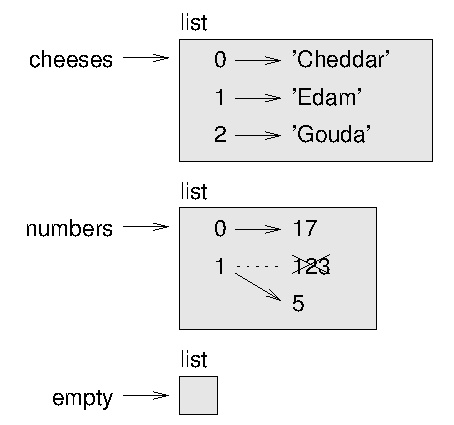
\includegraphics[scale=0.8]{figs/liststate.pdf}}
\caption{Diagramma di stato}
\label{fig.liststate}
\end{figure}

Le liste possono essere rappresentate da riquadri con la parola ``list'' all'esterno e i suoi elementi all'interno.  {\tt formaggi} si riferisce a una lista con tre elementi di indice 0, 1 e 2.
{\tt numeri} contiene due elementi; il diagramma mostra che il valore del secondo elemento è stato riassegnato da 123 a 5. {\tt vuota} si riferisce a una lista senza elementi.
\index{elemento, assegnazione}
\index{assegnazione!elemento}
\index{riassegnazione}

Gli indici delle liste funzionano nello stesso modo di quelli delle stringhe:

\begin{itemize}

\item L'indice può essere qualsiasi espressione di tipo intero.

\item Se tentate di leggere o modificare un elemento che non esiste, ottenete un messaggio d'errore {\tt IndexError}.
\index{eccezione!IndexError}
\index{IndexError}

\item Con un indice di valore negativo, si conta a ritroso dalla fine della
   lista.

\end{itemize}
\index{lista!indice}
\index{lista!appartenenza}
\index{appartenenza!lista}
\index{in, operatore}
\index{operatore!in}

Anche l'operatore {\tt in} funziona con le liste:

\begin{verbatim}
>>> formaggi = ['Cheddar', 'Edam', 'Gouda']
>>> 'Edam' in formaggi
True
>>> 'Brie' in formaggi
False
\end{verbatim}


\section{Attraversamento di una lista}
\index{lista!attraversamento}
\index{attraversamento!lista}
\index{for, ciclo}
\index{ciclo!for}
\index{istruzione!for}

Il modo più frequente di attraversare gli elementi di una lista è un ciclo {\tt for}. Anche qui, la sintassi è la stessa delle stringhe:

\begin{verbatim}
for formaggio in formaggi:
    print(formaggio)
\end{verbatim}
%
Questo metodo funziona bene per leggere gli elementi di una lista, ma se volete scrivere o aggiornare degli elementi vi servono gli indici. Un modo per farlo è usare una combinazione delle funzioni predefinite {\tt range} e {\tt len}:
\index{ciclo!con indici}
\index{indice!nei cicli}

\begin{verbatim}
for i in range(len(numeri)):
    numeri[i] = numeri[i] * 2
\end{verbatim}
%
Questo ciclo attraversa la lista e aggiorna tutti gli elementi. {\tt len}
restituisce il numero di elementi della lista.  {\tt range} restituisce una lista di indici da 0 a $n-1$, dove $n$ è la lunghezza della lista. Ad ogni ripetizione del ciclo, {\tt i} prende l'indice dell'elemento successivo. L'istruzione di assegnazione nel corpo usa {\tt i} per leggere il vecchio valore dell'elemento e assegnare quello nuovo.
\index{elemento!aggiornamento}
\index{aggiornamento!elemento}

Un ciclo {\tt for} su una lista vuota non esegue mai il corpo:

\begin{verbatim}
for x in []:
    print('Questo non succede mai.')
\end{verbatim}
%
Sebbene una lista possa contenerne un'altra, quella nidificata conta sempre come un singolo elemento. Quindi la lunghezza di questa lista è quattro:
\index{nidificata, lista}
\index{lista!nidificata}

\begin{verbatim}
['spam', 1, ['Brie', 'Roquefort', 'Pol le Veq'], [1, 2, 3]]
\end{verbatim}



\section{Operazioni sulle liste}
\index{lista!operazione}

L'operatore {\tt +} concatena delle liste:
\index{concatenamento!lista}
\index{lista!concatenamento}

\begin{verbatim}
>>> a = [1, 2, 3]
>>> b = [4, 5, 6]
>>> c = a + b
>>> c
[1, 2, 3, 4, 5, 6]
\end{verbatim}
%
L'operatore {\tt *} ripete una lista per un dato numero di volte:
\index{ripetizione!lista}
\index{lista!ripetizione}

\begin{verbatim}
>>> [0] * 4
[0, 0, 0, 0]
>>> [1, 2, 3] * 3
[1, 2, 3, 1, 2, 3, 1, 2, 3]
\end{verbatim}
%
Il primo esempio ripete {\tt [0]} per quattro volte. Il secondo ripete la lista {\tt [1, 2, 3]} per tre volte.


\section{Slicing delle liste}
\index{slicing!operatore di}
\index{operatore!di slicing}
\index{indice!slicing}
\index{lista!slicing}
\index{slicing!lista}

Anche l'operazione di slicing funziona sulle liste:

\begin{verbatim}
>>> t = ['a', 'b', 'c', 'd', 'e', 'f']
>>> t[1:3]
['b', 'c']
>>> t[:4]
['a', 'b', 'c', 'd']
>>> t[3:]
['d', 'e', 'f']
\end{verbatim}
%
Se omettete il primo indice, lo slicing comincia dall'inizio, mentre se manca il secondo, termina alla fine. Se vengono omessi entrambi, lo slicing è una copia dell'intera lista.
\index{lista!copia}
\index{slicing!copia}
\index{copia!slicing}

\begin{verbatim}
>>> t[:]
['a', 'b', 'c', 'd', 'e', 'f']
\end{verbatim}
%
Dato che le liste sono mutabili, spesso è utile farne una copia prima di eseguire operazioni che le modificano.
\index{mutabilità}

Un operatore di slicing sul lato sinistro di un'assegnazione, permette di aggiornare più elementi.
\index{slicing!aggiornamento}
\index{aggiornamento!slicing}

\begin{verbatim}
>>> t = ['a', 'b', 'c', 'd', 'e', 'f']
>>> t[1:3] = ['x', 'y']
>>> t
['a', 'x', 'y', 'd', 'e', 'f']
\end{verbatim}
%


\section{Metodi delle liste}
\index{lista!metodi}
\index{metodi delle liste}

Python fornisce dei metodi che operano sulle liste. Ad esempio,
{\tt append} aggiunge un nuovo elemento in coda alla lista:
\index{append, metodo}
\index{metodo!append}

\begin{verbatim}
>>> t = ['a', 'b', 'c']
>>> t.append('d')
>>> t
['a', 'b', 'c', 'd']
\end{verbatim}
%
{\tt extend} prende una lista come argomento e accoda tutti i suoi elementi:
\index{extend, metodo}
\index{metodo!extend}

\begin{verbatim}
>>> t1 = ['a', 'b', 'c']
>>> t2 = ['d', 'e']
>>> t1.extend(t2)
>>> t1
['a', 'b', 'c', 'd', 'e']
\end{verbatim}
%
Questo esempio lascia immutata la lista {\tt t2}.

{\tt sort} dispone gli elementi della lista in ordine crescente:
\index{sort, metodo}
\index{metodo!sort}

\begin{verbatim}
>>> t = ['d', 'c', 'e', 'b', 'a']
>>> t.sort()
>>> t
['a', 'b', 'c', 'd', 'e']
\end{verbatim}
%
La maggior parte dei metodi delle liste sono vuoti: modificano la lista e restituiscono {\tt None}. Se scrivete accidentalmente  {\tt t = t.sort()}, il risultato vi deluderà.
\index{metodo!vuoto}
\index{None, valore speciale}
\index{valore speciale!None}


\section{Mappare, filtrare e ridurre}
\label{filter}

Per sommare tutti i numeri in una lista, potete usare un ciclo come questo:

% see add.py

\begin{verbatim}
def somma_tutti(t):
    totale = 0
    for x in t:
        totale += x
    return totale
\end{verbatim}
%
{\tt totale} è inizializzato a 0. Ad ogni ripetizione del ciclo,
{\tt x} prende un elemento dalla lista. L'operatore {\tt +=} è una forma abbreviata per aggiornare una variabile. Questa
{\bf istruzione di assegnazione potenziata},
\index{aggiornamento!operatore di}
\index{operatore!di aggiornamento}
\index{assegnazione!potenziata}
\index{potenziata, assegnazione}

\begin{verbatim}
    totale += x
\end{verbatim}
%
è equivalente a

\begin{verbatim}
    totale = totale + x
\end{verbatim}
%
Man mano che il ciclo lavora, {\tt totale} accumula la somma degli elementi; una variabile usata in questo modo è detta anche {\bf accumulatore}.
\index{accumulatore!somma}

Sommare gli elementi di una lista è un'operazione talmente comune che Python contiene una apposita funzione predefinita, {\tt sum}:

\begin{verbatim}
>>> t = [1, 2, 3]
>>> sum(t)
6
\end{verbatim}
%
Una simile operazione che compatta una sequenza di elementi in un singolo valore, è chiamata {\bf riduzione}.
\index{riduzione, schema}
\index{schema!riduzione}
\index{attraversamento}

Talvolta è necessario attraversare una lista per costruirne contemporaneamente un'altra. Per esempio, la funzione seguente prende una lista di stringhe e restituisce una nuova lista che contiene le stesse stringhe in lettere maiuscole:

\begin{verbatim}
def tutte_maiuscole(t):
    res = []
    for s in t:
        res.append(s.capitalize())
    return res
\end{verbatim}
%
{\tt res} è inizializzata come una lista vuota; ad ogni ripetizione del ciclo viene accodato un elemento. Pertanto {\tt res} è una sorta di accumulatore.
\index{accumulatore!lista}

Un'operazione come quella di \verb"tutte_maiuscole" è chiamata anche {\bf
mappa}: applica una funzione (in questo caso il metodo {\tt
capitalize}) su ciascun elemento di una sequenza.
\index{mappa, schema}
\index{schema!mappa}
\index{filtro, schema}
\index{schema!filtro}

Un'altra operazione frequente è la selezione di alcuni elementi di una lista per formare una sottolista. Per esempio, la seguente funzione prende una lista di stringhe e restituisce una lista che contiene solo le stringhe scritte in lettere maiuscole:

\begin{verbatim}
def solo_maiuscole(t):
    res = []
    for s in t:
        if s.isupper():
            res.append(s)
    return res
\end{verbatim}
%
{\tt isupper} è un metodo delle stringhe che restituisce {\tt True} se la stringa contiene solo lettere maiuscole.

Un'operazione come quella di \verb"solo_maiuscole" è chiamata {\bf filtro} perché seleziona solo alcuni elementi, filtrando gli altri.

La maggior parte delle operazioni sulle liste possono essere espresse come combinazioni di mappa, filtro e riduzione.

\section{Cancellare elementi}
\index{elemento!cancellazione}
\index{cancellare, elementi di lista}

Ci sono vari modi per cancellare elementi da una lista. Se conoscete l'indice dell'elemento desiderato, potete usare
{\tt pop}:
\index{pop, metodo}
\index{metodo!pop}

\begin{verbatim}
>>> t = ['a', 'b', 'c']
>>> x = t.pop(1)
>>> t
['a', 'c']
>>> x
'b'
\end{verbatim}
%
{\tt pop} modifica la lista e restituisce l'elemento che è stato rimosso. Se omettete l'indice, il metodo cancella e restituisce l'ultimo elemento della lista.

Se non vi serve il valore rimosso, potete usare l'operatore {\tt del}:
\index{del, operatore}
\index{operatore!del}

\begin{verbatim}
>>> t = ['a', 'b', 'c']
>>> del t[1]
>>> t
['a', 'c']
\end{verbatim}
%

Se conoscete l'elemento da rimuovere ma non il suo indice, potete usare {\tt remove}:
\index{remove, metodo}
\index{metodo!remove}

\begin{verbatim}
>>> t = ['a', 'b', 'c']
>>> t.remove('b')
>>> t
['a', 'c']
\end{verbatim}
%
Il valore di ritorno di {\tt remove} è {\tt None}.
\index{None, valore speciale}
\index{valore speciale!None}

Per cancellare più di un elemento potete usare {\tt del} con lo slicing:

\begin{verbatim}
>>> t = ['a', 'b', 'c', 'd', 'e', 'f']
>>> del t[1:5]
>>> t
['a', 'f']
\end{verbatim}
%
Come di consueto, lo slicing seleziona gli elementi fino al secondo indice escluso.

\section{Liste e stringhe}
\index{lista}
\index{stringa}
\index{sequenza}

Una stringa è una sequenza di caratteri e una lista è una sequenza di valori, ma una lista di caratteri non è la stessa cosa di una stringa. Per convertire una stringa in una lista di caratteri, potete usare {\tt list}:
\index{list, funzione}
\index{funzione!list}

\begin{verbatim}
>>> s = 'spam'
>>> t = list(s)
>>> t
['s', 'p', 'a', 'm']
\end{verbatim}
%
Poiché {\tt list} è una funzione predefinita, va evitato di chiamare una variabile con questo nome. Personalmente evito anche {\tt l} perché somiglia troppo a {\tt 1}.  Ecco perché di solito uso {\tt t}.

La funzione {\tt list} separa una stringa in singole lettere. Se invece volete spezzare una stringa nelle singole parole, usate il metodo {\tt split}:
\index{split, metodo}
\index{metodo!split}

\begin{verbatim}
>>> s = 'profonda nostalgia dei fiordi'
>>> t = s.split()
>>> t
['profonda', 'nostalgia', 'dei', 'fiordi']
\end{verbatim}
%
Un argomento opzionale chiamato {\bf delimitatore} specifica quale carattere va considerato come separatore delle parole. L'esempio che segue usa il trattino come separatore:
\index{argomento!opzionale}
\index{delimitatore}

\begin{verbatim}
>>> s = 'spam-spam-spam'
>>> delimita = '-'
>>> t = s.split(delimita)
>>> t
['spam', 'spam', 'spam']
\end{verbatim}
%
{\tt join} è l'inverso di {\tt split}: prende una lista di stringhe e concatena gli elementi.  {\tt join} è un metodo delle stringhe, quindi lo dovete invocare per mezzo del delimitatore e passare la lista come parametro:
\index{join, metodo}
\index{metodo!join}
\index{concatenamento}

\begin{verbatim}
>>> t = ['profonda', 'nostalgia', 'dei', 'fiordi']
>>> delimita = ' '
>>> s = delimita.join(t)
>>> s
'profonda nostalgia dei fiordi'
\end{verbatim}
%
In questo caso il delimitatore è uno spazio, quindi
{\tt join} aggiunge uno spazio tra le parole. Per concatenare delle stringhe senza spazi, basta usare come delimitatore la stringa vuota \verb"''".
\index{stringa!vuota}


\section{Oggetti e valori}
\label{equivalence}
\index{oggetto}
\index{valore}

Se eseguiamo queste istruzioni di assegnazione:

\begin{verbatim}
a = 'banana'
b = 'banana'
\end{verbatim}
%
Sappiamo che {\tt a} e {\tt b} si riferiscono a una stringa, ma non sappiamo se si riferiscono alla {\em stessa} stringa.
Ci sono due possibili stati, illustrati in Figura~\ref{fig.list1}.
\index{alias}

\begin{figure}
\centerline
{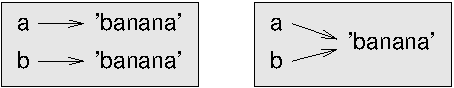
\includegraphics[scale=0.8]{figs/list1.pdf}}
\caption{Diagramma di stato.}
\label{fig.list1}
\end{figure}


In un caso, {\tt a} e {\tt b} si riferiscono a due oggetti diversi che hanno lo stesso valore. Nell'altro, si riferiscono allo stesso oggetto.
\index{is, operatore}
\index{operatore!is}

Per controllare se due variabili si riferiscono allo stesso oggetto, potete usare l'operatore {\tt is}.

\begin{verbatim}
>>> a = 'banana'
>>> b = 'banana'
>>> a is b
True
\end{verbatim}
%
In questo esempio, Python ha creato un unico oggetto stringa, e sia {\tt a} che {\tt b} fanno riferimento ad esso.

Ma se create due liste, ottenete due oggetti distinti:

\begin{verbatim}
>>> a = [1, 2, 3]
>>> b = [1, 2, 3]
>>> a is b
False
\end{verbatim}
%
Quindi il diagramma di stato somiglia a quello di Figura~\ref{fig.list2}.
\index{diagramma!di stato}

\begin{figure}
\centerline
{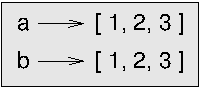
\includegraphics[scale=0.8]{figs/list2.pdf}}
\caption{Diagramma di stato.}
\label{fig.list2}
\end{figure}

In quest'ultimo caso si dice che le due liste sono {\bf equivalenti},
perché contengono gli stessi elementi, ma non {\bf identiche}, perché non sono lo stesso oggetto.
Se due oggetti sono identici, sono anche equivalenti, ma se sono equivalenti non sono necessariamente identici.
\index{equivalente}
\index{identità}

Fino ad ora abbiamo usato ``oggetto'' e ``valore'' indifferentemente, ma è più preciso dire che un oggetto ha un valore.  Se valutate {\tt [1,2,3]}, ottenete un oggetto lista il cui valore è una sequenza di interi. Se un'altra lista contiene gli stessi elementi, diciamo che ha lo stesso valore, ma non che è lo stesso oggetto.
\index{oggetto}
\index{valore}


\section{Alias}
\index{alias}
\index{riferimento!alias}

Se la variabile {\tt a} si riferisce a un oggetto e assegnate {\tt b = a},
allora entrambe le variabili si riferiscono allo stesso oggetto.

\begin{verbatim}
>>> a = [1, 2, 3]
>>> b = a
>>> b is a
True
\end{verbatim}
%
Il diagramma di stato è quello in Figura~\ref{fig.list3}.
\index{diagramma!di stato}

\begin{figure}
\centerline
{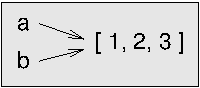
\includegraphics[scale=0.8]{figs/list3.pdf}}
\caption{Diagramma di stato.}
\label{fig.list3}
\end{figure}

L'associazione tra una variabile e un oggetto è chiamato {\bf
riferimento}. In questo esempio ci sono due riferimenti allo stesso oggetto.
\index{riferimento}

Un oggetto che ha più di un riferimento ha anche più di un nome, e si dice quindi che l'oggetto ha degli {\bf alias}.
\index{mutabilità}

Se l'oggetto munito di alias è mutabile, i cambiamenti provocati da un alias si riflettono anche sull'altro:

\begin{verbatim}
>>> b[0] = 42
>>> a
[42, 2, 3]
\end{verbatim}
%
Sebbene questo comportamento possa essere utile, è anche fonte di errori. In genere è più sicuro evitare gli alias quando si sta lavorando con oggetti mutabili.
\index{immutabilità}

Per gli oggetti immutabili come le stringhe, gli alias non sono un problema. In questo esempio:

\begin{verbatim}
a = 'banana'
b = 'banana'
\end{verbatim}
%
Non fa quasi mai differenza se {\tt a} e {\tt b} facciano riferimento alla stessa stringa o meno.


\section{Liste come argomenti}
\label{list.arguments}
\index{lista!come argomento}
\index{argomento}
\index{argomento!lista}
\index{riferimento}
\index{parametro}

Quando passate una lista a una funzione, questa riceve un riferimento alla lista. Se la funzione modifica la lista, il chiamante vede la modifica. Per esempio, \verb"decapita" rimuove il primo elemento di una lista:

\begin{verbatim}
def decapita(t):
    del t[0]
\end{verbatim}
%
Vediamo come si usa:

\begin{verbatim}
>>> lettere = ['a', 'b', 'c']
>>> decapita(lettere)
>>> lettere
['b', 'c']
\end{verbatim}
%
Il parametro {\tt t} e la variabile {\tt lettere} sono due alias dello stesso oggetto. Il diagramma di stack è riportato in Figura~\ref{fig.stack5}.
\index{diagramma!di stack}

\begin{figure}
\centerline
{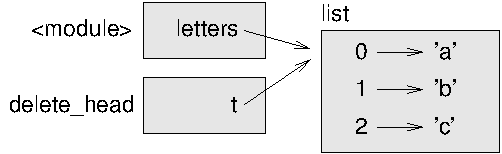
\includegraphics[scale=0.8]{figs/stack5.pdf}}
\caption{Diagramma di stack.}
\label{fig.stack5}
\end{figure}


Dato che la lista è condivisa da due frame, la disegno in mezzo.

È importante distinguere tra operazioni che modificano le liste e operazioni che creano nuove liste. Per esempio il metodo {\tt append} modifica una lista, ma l'operatore {\tt +} ne crea una nuova.

Ecco un esempio che usa {\tt append}:
\index{append, metodo}
\index{metodo!append}
\index{lista!concatenamento}
\index{concatenamento!lista}
%
\begin{verbatim}
>>> t1 = [1, 2]
>>> t2 = t1.append(3)
>>> t1
[1, 2, 3]
>>> t2
None
\end{verbatim}
%
Il valore di ritorno di {\tt append} è {\tt None}.

Un esempio di utilizzo dell'operatore {\tt +}:
%
\begin{verbatim}
>>> t3 = t1 + [4]
>>> t1
[1, 2, 3]
>>> t3
[1, 2, 3, 4]
\end{verbatim}
%
Il risultato è una nuova lista, e la lista di origine resta immutata.

Questa differenza è importante quando scrivete delle funzioni che devono modificare delle liste. Per esempio, questa funzione
{\em non} cancella il primo elemento della lista:
%
\begin{verbatim}
def non_decapita(t):
    t = t[1:]              # SBAGLIATO!
\end{verbatim}
%
L'operatore di slicing crea una nuova lista e l'assegnazione fa in modo che {\tt t} si riferisca ad essa, ma tutto ciò non ha effetti sul chiamante.
\index{slicing!operatore di}
\index{operatore!di slicing}
%
\begin{verbatim}
>>> t4 = [1, 2, 3]
>>> non_decapita(t4)
>>> t4
[1, 2, 3]
\end{verbatim}
%
Alla chiamata di \verb"non_decapita", {\tt t} e {\tt t4} fanno riferimento
alla stessa lista.  Alla fine, {\tt t} fa riferimento ad una nuova lista,
mentre {\tt t4} continua a fare riferimento alla stessa lista, non modificata.

Un'alternativa valida è scrivere una funzione che crea e restituisce una nuova lista. Per esempio, {\tt ritaglia} restituisce tutti gli elementi di una lista tranne il primo:

\begin{verbatim}
def ritaglia(t):
    return t[1:]
\end{verbatim}
%
Questa funzione lascia intatta la lista di origine. Ecco come si usa:

\begin{verbatim}
>>> lettere = ['a', 'b', 'c']
>>> resto = ritaglia(lettere)
>>> resto
['b', 'c']
\end{verbatim}



\section{Debug}
\index{debug}

Un uso poco accurato delle liste (e degli altri oggetti mutabili) può portare a lunghe ore di debug. Ecco alcune delle trappole più comuni e i modi per evitarle:

\begin{enumerate}

\item La maggior parte dei metodi delle liste modificano l'argomento e restituiscono {\tt None}.  È il comportamento opposto dei metodi delle stringhe, che restituiscono una nuova stringa e lasciano immutato l'originale.

Se siete abituati a scrivere il codice per le stringhe così:

\begin{verbatim}
parola = parola.strip()
\end{verbatim}

Può venire spontaneo di scrivere il codice per le liste così:

\begin{verbatim}
t = t.sort()           # SBAGLIATO!
\end{verbatim}
\index{sort, metodo}
\index{metodo!sort}

Ma poiché {\tt sort} restituisce {\tt None}, l'operazione successiva che eseguite su {\tt t} con tutta probabilità fallirà.

Prima di usare i metodi delle liste e gli operatori, leggetene attentamente la documentazione e fate una prova in modalità interattiva.


\item Scegliete un costrutto e usate sempre quello.

Una parte dei problemi delle liste deriva dal fatto che ci sono molti modi per fare le stesse cose. Per esempio, per rimuovere un elemento da una lista potete usare {\tt pop}, {\tt remove}, {\tt del}, oppure lo slicing.

Per aggiungere un elemento potete usare il metodo {\tt append} o l'operatore {\tt +}. Supponendo che {\tt t} sia una lista e {\tt x} un elemento, le espressioni seguenti vanno entrambe bene:

\begin{verbatim}
t.append(x)
t = t + [x]
\end{verbatim}

Mentre queste sono sbagliate:

\begin{verbatim}
t.append([x])          # SBAGLIATO!
t = t.append(x)        # SBAGLIATO!
t + [x]                # SBAGLIATO!
t = t + x              # SBAGLIATO!
\end{verbatim}

Provate ognuno di questi esempi in modalità interattiva per verificare quello che fanno. Noterete che solo l'ultima espressione causa un errore di esecuzione; le altre sono consentite, ma fanno la cosa sbagliata.


\item Fate copie per evitare gli alias.
\index{alias!copiare per evitare}
\index{copia!per evitare alias}

Se volete usare un metodo come {\tt sort} che modifica l'argomento, ma anche mantenere inalterata la lista di origine, potete farne una copia.

\begin{verbatim}
>>> t = [3, 1, 2]
>>> t2 = t[:]
>>> t2.sort()
>>> t
[3, 1, 2]
>>> t2
[1, 2, 3]
\end{verbatim}

In questo esempio, si può anche usare la funzione predefinita {\tt sorted},
che restituisce una nuova lista ordinata e lascia intatta quella di origine.
\index{sorted!funzione}
\index{funzione!sorted}

\begin{verbatim}
>>> t2 = sorted(t)
>>> t
[3, 1, 2]
>>> t2
[1, 2, 3]
\end{verbatim}

\end{enumerate}


\section{Glossario}

\begin{description}

\item[lista:] Una sequenza di valori.
\index{lista}

\item[elemento:] Uno dei valori in una lista (o in altri tipi di sequenza).
\index{elemento}

\item[lista nidificata:] Lista che è contenuta come elemento in un'altra lista.
\index{lista!nidificata}

\item[accumulatore:] Variabile usata in un ciclo per sommare cumulativamente un risultato.
\index{accumulatore}

\item[assegnazione potenziata:] Istruzione che aggiorna un valore di una variabile usando un operatore come \verb"+=".
\index{assegnazione!potenziata}
\index{attraversamento}

\item[riduzione:] Schema di calcolo che attraversa una sequenza e ne accumula gli elementi in un singolo risultato.
\index{riduzione, schema}
\index{schema!riduzione}

\item[mappa:] Schema di calcolo che attraversa una sequenza ed esegue una stessa operazione su ciascun elemento della sequenza.
\index{mappa, schema}
\index{schema!mappa}

\item[filtro:] Schema di calcolo che attraversa una lista e seleziona solo gli elementi che soddisfano un dato criterio.
\index{filtro, schema}
\index{schema!filtro}

\item[oggetto:] Qualcosa a cui una variabile può fare riferimento. Un oggetto ha un tipo e un valore.
\index{oggetto}

\item[equivalente:] Avente lo stesso valore.
\index{equivalente}

\item[identico:] Essere lo stesso oggetto (implica anche l'equivalenza).
\index{identico}

\item[riferimento:] L'associazione tra una variabile e il suo valore.
\index{riferimento}

\item[alias:] Due o più variabili che si riferiscono allo stesso oggetto, con nomi diversi.
\index{alias}

\item[delimitatore:] Carattere o stringa usato per indicare i punti dove una stringa deve essere spezzata.
\index{delimitatore}

\end{description}


\section{Esercizi}

Potete scaricare le soluzioni degli esercizi seguenti all'indirizzo
\url{http://thinkpython2.com/code/list_exercises.py}.

\vspace{0.2in}
\begin{exercise}

Scrivete una funzione di nome \verb"somma_nidificata" che prenda una lista di liste di numeri interi e sommi gli elementi di tutte le liste nidificate.
Esempio:

\begin{verbatim}
>>> t = [[1, 2], [3], [4, 5, 6]]
>>> somma_nidificata(t)
21
\end{verbatim}

\end{exercise}

\vspace{0.2in}
\begin{exercise}
\label{cumulative}
\index{cumulativa, somma}

Scrivete una funzione di nome \verb"somma_cumulata" che prenda una lista di numeri e restituisca la somma cumulata, cioè una nuova lista dove l'$i$-esimo elemento è la somma dei primi $i+1$ elementi della lista di origine. Per esempio:

\begin{verbatim}
>>> t = [1, 2, 3]
>>> somma_cumulata(t)
[1, 3, 6]
\end{verbatim}

\end{exercise}

\vspace{0.2in}
\begin{exercise}

Scrivete una funzione di nome \verb"mediani" che prenda una lista e restituisca una nuova lista che contenga tutti gli elementi, esclusi il primo e l'ultimo.
Esempio:

\begin{verbatim}
>>> t = [1, 2, 3, 4]
>>> mediani(t)
[2, 3]
\end{verbatim}

\end{exercise}

\vspace{0.2in}
\begin{exercise}

Scrivete una funzione di nome \verb"tronca" che prenda una lista, la modifichi togliendo il primo e l'ultimo elemento, e restituisca {\tt None}.
Esempio:

\begin{verbatim}
>>> t = [1, 2, 3, 4]
>>> tronca(t)
>>> t
[2, 3]
\end{verbatim}
\end{exercise}

\vspace{0.2in}
\begin{exercise}
Scrivete una funzione di nome \verb"ordinata" che prenda una lista come parametro e restituisca {\tt True} se la lista è ordinata in senso crescente, {\tt False} altrimenti. Esempio:

\begin{verbatim}
>>> ordinata([1, 2, 2])
True
>>> ordinata(['b', 'a'])
False
\end{verbatim}

\end{exercise}

\vspace{0.2in}
\begin{exercise}
\label{anagram}
\index{anagramma}

Due parole sono anagrammi se potete ottenerle riordinando le lettere di cui sono composte. Scrivete una funzione di nome \verb"anagramma"
che riceva due stringhe e restituisca {\tt True} se sono anagrammi.
\end{exercise}

\vspace{0.2in}
\begin{exercise}
\label{duplicate}
\index{duplicato}
\index{unicità}

Scrivete una funzione di nome \verb"ha_duplicati" che richieda una lista e restituisca {\tt True} se contiene elementi che compaiono più di una volta. Non deve modificare la lista di origine.

\end{exercise}

\vspace{0.2in}
\begin{exercise}

Questo è un esercizio sul cosiddetto ``Paradosso del compleanno''; potete approfondirlo leggendo \url{http://it.wikipedia.org/wiki/Paradosso_del_compleanno}.
\index{compleanno, paradosso del}

Se in una classe ci sono 23 studenti, quante probabilità ci sono che due di loro compiano gli anni lo stesso giorno? Potete stimare questa probabilità generando alcuni campioni a caso di 23 date e controllando le corrispondenze. Suggerimento: per generare date in modo casuale usate la funzione {\tt randint} nel modulo {\tt random}.
\index{random, modulo}
\index{modulo!random}
\index{randint, funzione}
\index{funzione!randint}

Potete scaricare la mia soluzione da \url{http://thinkpython2.com/code/birthday.py}.

\end{exercise}

\vspace{0.2in}
\begin{exercise}
\index{append, metodo}
\index{metodo!append}
\index{lista!concatenamento}
\index{concatenamento!lista}

Scrivete una funzione che legga il file {\tt words.txt} e crei una lista in cui ogni parola è un elemento. Scrivete due versioni della funzione, una che usi il metodo {\tt append} e una il costrutto {\tt t = t + [x]}. Quale richiede più tempo di esecuzione? Perché?

Soluzione: \url{http://thinkpython2.com/code/wordlist.py}.

\end{exercise}

\vspace{0.2in}
\begin{exercise}
\label{wordlist1}
\label{bisection}
\index{appartenenza!ricerca binaria}
\index{ricerca!binaria}
\index{appartenenza!ricerca binaria}
\index{ricerca!binaria}

Per controllare se una parola è contenuta in un elenco, è possibile usare l'operatore {\tt in}, ma è un metodo lento, perché ricerca le parole seguendo il loro ordine.

Dato che le parole sono in ordine alfabetico, possiamo accelerare l'operazione con una ricerca binaria (o per bisezione), che è un po' come cercare una parola nel vocabolario.
Partite nel mezzo e controllate se la parola che cercate viene prima o dopo la parola di metà elenco. Se prima, cercherete nella prima metà nello stesso modo, se dopo, cercherete nella seconda metà.

Ad ogni passaggio, dimezzate lo spazio di ricerca. Se l'elenco ha 113.809 parole, ci vorranno circa 17 passaggi per trovare la parola o concludere che non c'è.

Scrivete una funzione di nome {\tt bisezione} che richieda una lista ordinata e un valore da ricercare, e restituisca {\tt True} se la parola fa parte della lista, o {\tt False} se non è presente.
\index{bisect, modulo}
\index{modulo!bisect}

Oppure, potete leggere la documentazione del modulo {\tt bisect} e usare quello!  Soluzione: \url{http://thinkpython2.com/code/inlist.py}.

\end{exercise}

\vspace{0.2in}
\begin{exercise}
\index{bifronte, parola}

Una coppia di parole è ``bifronte'' se l'una si legge nel verso opposto dell'altra. Scrivete un programma che trovi tutte le parole bifronti nella lista di parole.  Soluzione: \url{http://thinkpython2.com/code/reverse_pair.py}.

\end{exercise}

\vspace{0.2in}
\begin{exercise}
\index{incastro, parola}

Due parole si ``incastrano'' se, prendendo le loro lettere alternativamente  dall'una e dall'altra, si forma una nuova parola. Per esempio, le parole inglesi ``shoe'' and ``cold'' incastrandosi formano ``schooled''.


\begin{enumerate}

\item Scrivete un programma che trovi tutte le coppie di parole che possono incastrarsi. Suggerimento: non elaborate tutte le coppie!

\item Riuscite a trovare dei gruppi di tre parole che possono incastrarsi tra loro? Cioè, tre parole da cui, prendendo le lettere una ad una alternativamente, nell'ordine, si formi una nuova parola? (Es. ``ace'', ``bus'' e ``as'' danno ``abacuses'')

\end{enumerate}

Soluzione: \url{http://thinkpython2.com/code/interlock.py}.
Fonte: Questo esercizio è tratto da un esempio di \url{http://puzzlers.org}.
\end{exercise}


\chapter{Dizionari}

Questo capitolo illustra un altro tipo predefinito chiamato dizionario. I dizionari sono una delle migliori caratteristiche di Python; sono i mattoni che costituiscono molti eleganti ed efficienti algoritmi.

\section{Un dizionario è una mappatura}
\index{dizionario}
\index{tipo!dict}
\index{chiave}
\index{chiave-valore, coppia}
\index{indice}
Un {\bf dizionario} è simile ad una lista, ma è più generico. Infatti, mentre in una lista gli indici devono essere numeri interi, in un dizionario possono essere (quasi) di ogni tipo.

Un dizionario contiene una raccolta di indici, chiamati {\bf chiavi}, e una raccolta di valori. Ciascuna chiave è associata ad un unico valore. L'associazione tra una chiave e un valore è detta {\bf coppia chiave-valore} o anche {\bf elemento}.
\index{elemento}

In linguaggio matematico, un dizionario rappresenta una relazione di corrispondenza, o {\bf mappatura}, da una chiave a un valore, e si può dire pertanto che ogni chiave ``mappa in'' un valore.

Come esempio, costruiamo un dizionario che trasforma le parole dall'inglese all'italiano, quindi chiavi e valori saranno tutte delle stringhe.

La funzione {\tt dict} crea un nuovo dizionario privo di elementi. Siccome {\tt dict} è il nome di una funzione predefinita, è meglio evitare di usarlo come nome di variabile.
\index{dict, funzione}
\index{funzione!dict}

\begin{verbatim}
>>> eng2it = dict()
>>> eng2it
{}
\end{verbatim}

Le parentesi graffe, \verb"{}", rappresentano un dizionario vuoto. Per aggiungere elementi al dizionario, usate le parentesi quadre:
\index{graffe, parentesi}
\index{parentesi!graffe}

\begin{verbatim}
>>> eng2it['one'] = 'uno'
\end{verbatim}
%
Questa riga crea un elemento che contiene una corrispondenza dalla chiave
\verb"'one'" al valore \verb"'uno'".  Se stampiamo di nuovo il dizionario, vedremo ora una coppia chiave-valore separati da due punti:

\begin{verbatim}
>>> eng2it
{'one': 'uno'}
\end{verbatim}
%
Questo formato di output può essere anche usato per gli inserimenti. Ad esempio potete creare un nuovo dizionario con tre elementi:

\begin{verbatim}
>>> eng2it = {'one': 'uno', 'two': 'due', 'three': 'tre'}
\end{verbatim}
%
Se stampate ancora una volta {\tt eng2it}, avrete una sorpresa:

\begin{verbatim}
>>> eng2it
{'one': 'uno', 'three': 'tre', 'two': 'due'}
\end{verbatim}
%
L'ordine delle coppie chiave-valore non è necessariamente lo stesso. Se scrivete lo stesso esempio nel vostro computer, potreste ottenere un altro risultato ancora. In genere, l'ordine degli elementi di un dizionario è imprevedibile.

Ma questo non è un problema, perché gli elementi di un dizionario non sono indicizzati con degli indici numerici. Infatti, per cercare un valore si usano invece le chiavi:

\begin{verbatim}
>>> eng2it['two']
'due'
\end{verbatim}
%
La chiave \verb"'two'" corrisponde correttamente al valore \verb"'due'" e l'ordine degli elementi nel dizionario è ininfluente.

Se la chiave non è contenuta nel dizionario, viene generato un errore::
\index{eccezione!KeyError}
\index{KeyError}

\begin{verbatim}
>>> print(eng2it['four'])
KeyError: 'four'
\end{verbatim}
%
La funzione {\tt len} è applicabile ai dizionari, e restituisce il numero di coppie chiave-valore:
\index{len, funzione}
\index{funzione!len}

\begin{verbatim}
>>> len(eng2it)
3
\end{verbatim}
%
Anche l'operatore {\tt in} funziona con i dizionari: informa se qualcosa compare come {\em chiave} nel dizionario (non è condizione sufficiente che sia contenuto come valore).
\index{appartenenza!dizionario}
\index{in, operatore}
\index{operatore!in}

\begin{verbatim}
>>> 'one' in eng2it
True
>>> 'uno' in eng2it
False
\end{verbatim}
%
Per controllare invece se qualcosa compare come valore, potete usare il metodo {\tt values}, che restituisce una raccolta dei valori, e quindi usare l'operatore {\tt in}:
\index{values, metodo}
\index{metodo!values}

\begin{verbatim}
>>> vals = eng2it.values()
>>> 'uno' in vals
True
\end{verbatim}
%
L'operatore {\tt in} utilizza algoritmi diversi per liste e dizionari. Per le prime, ne ricerca gli elementi in base all'ordine, come nel Paragrafo~\ref{find}.  Se la lista si allunga, anche il tempo di ricerca si allunga in proporzione. Per i secondi, Python usa un algoritmo chiamato {\bf tabella hash} che ha notevoli proprietà: l'operatore {\tt in} impiega sempre circa lo stesso tempo, indipendentemente da quanti elementi contiene il dizionario. Rimando la spiegazione di come ciò sia possibile all'Appendice~\ref{hashtable}: per capirla, occorre prima leggere qualche altro capitolo.
\index{tabella hash}

\section{Il dizionario come raccolta di contatori}
\label{histogram}
\index{contatore}

Supponiamo che vi venga data una stringa e che vogliate contare quante volte vi compare ciascuna lettera. Ci sono alcuni modi per farlo:

\begin{enumerate}

\item Potete creare 26 variabili, una per lettera dell'alfabeto. Quindi, fare un attraversamento della stringa e per ciascun carattere incrementate il contatore corrispondente, magari usando delle condizioni in serie.

\item Potete creare una lista di 26 elementi, quindi convertire ogni carattere in un numero (usando la funzione predefinita {\tt ord}), utilizzare il numero come indice e incrementare il contatore corrispondente.

\item Potete creare un dizionario con i caratteri come chiavi e i contatori come valore corrispondente. La prima volta che incontrate un carattere, lo aggiungete come elemento al dizionario. Successivamente, incrementerete il valore dell'elemento esistente.

\end{enumerate}

Ciascuna di queste opzioni esegue lo stesso calcolo, ma lo implementa in modo diverso.
\index{implementazione}

Un'{\bf implementazione} è un modo per effettuare un'elaborazione. Le implementazioni non sono tutte uguali, alcune sono migliori di altre: per esempio, un vantaggio dell'implementazione con il dizionario è che non serve sapere in anticipo quali lettere ci siano nella stringa e quali no, dobbiamo solo fare spazio per le lettere che compariranno effettivamente.

Ecco come potrebbe essere scritto il codice:

\begin{verbatim}
def istogramma(s):
    d = dict()
    for c in s:
        if c not in d:
            d[c] = 1
        else:
            d[c] += 1
    return d
\end{verbatim}
%
Il nome di questa funzione è {\tt istogramma}, che è un termine statistico per indicare un insieme di contatori (o frequenze).
\index{istogramma}
\index{frequenza}
\index{attraversamento}

La prima riga della funzione crea un dizionario vuoto. Il ciclo {\tt for}  attraversa la stringa. Ad ogni ripetizione, se il carattere {\tt c} non compare nel dizionario crea un nuovo elemento di chiave {\tt c} e valore iniziale 1 (dato che incontra questa lettera per la prima volta). Se invece {\tt c} è già presente, incrementa {\tt d[c]} di una unità.
\index{istogramma}

Vediamo come funziona:

\begin{verbatim}
>>> h = istogramma('brontosauro')
>>> h
{'a': 1, 'b': 1, 'o': 3, 'n': 1, 's': 1, 'r': 2, 'u': 1, 't': 1}
\end{verbatim}
%
L'istogramma indica che le lettere \verb"'a'" e \verb"'b'"
compaiono una volta, la \verb"'o'" tre volte e così via.

I dizionari supportano il metodo {\tt get} che richiede una chiave e un valore predefinito. Se la chiave è presente nel dizionario, {\tt get} restituisce il suo valore corrispondente, altrimenti restituisce il valore predefinito. Per esempio:
\index{get, metodo}
\index{metodo!get}

\begin{verbatim}
>>> h = istogramma('a')
>>> h
{'a': 1}
>>> h.get('a', 0)
1
>>> h.get('b', 0)
0
\end{verbatim}
%
Come esercizio, usate {\tt get} per scrivere {\tt istogramma} in modo più compatto. Dovreste riuscire a fare a meno dell'istruzione {\tt if}.


\section{Cicli e dizionari}
\index{dizionario!ciclo con}
\index{ciclo!con dizionario}
\index{attraversamento}

Se usate un dizionario in un ciclo {\tt for}, quest'ultimo attraversa le chiavi del dizionario. Per esempio, \verb"stampa_isto" visualizza ciascuna chiave e il valore corrispondente:

\begin{verbatim}
def stampa_isto(h):
    for c in h:
        print(c, h[c])
\end{verbatim}
%
Ecco come risulta l'output:

\begin{verbatim}
>>> h = istogramma('parrot')
>>> stampa_isto(h)
a 1
p 1
r 2
t 1
o 1
\end{verbatim}
%
Di nuovo, le chiavi sono alla rinfusa. Per attraversare le chiavi disponendole
in ordine, si può utilizzare la funzione predefinita {\tt sorted}:
\index{sorted, funzione}
\index{funzione!sorted}

\begin{verbatim}
>>> for chiave in sorted(h):
...     print(chiave, h[chiave])
a 1
o 1
p 1
r 2
t 1
\end{verbatim}




\section{Lookup inverso}
\label{raise}
\index{dizionario!lookup}
\index{dizionario!lookup inverso}
\index{lookup!dizionario}
\index{lookup inverso, dizionario}

Dato un dizionario {\tt d} e una chiave {\tt k}, è facile trovare il valore corrispondente alla chiave: {\tt v = d[k]}.  Questa operazione è chiamata {\bf lookup}.

Ma se invece volete trovare la chiave {\tt k} conoscendo il valore {\tt v}?
Avete due problemi: primo, ci possono essere più chiavi che corrispondono al valore {\tt v}.  A seconda dell'applicazione, potete riuscire a trovarne uno, oppure può essere necessario ricavare una lista che li contenga tutti. Secondo, non c'è una sintassi semplice per fare un {\bf lookup inverso}; dovete impostare una ricerca.

Ecco una funzione che richiede un valore e restituisce la prima chiave a cui corrisponde quel valore:

\begin{verbatim}
def inverso_lookup(d, v):
    for k in d:
        if d[k] == v:
            return k
    raise LookupError()
\end{verbatim}
%
Questa funzione è un altro esempio di schema di ricerca, ma usa un'istruzione che non abbiamo mai visto prima, {\tt raise}.  L'istruzione {\tt raise}
solleva un'eccezione; in questo caso genera un errore {\tt LookupError}, che è un eccezione predefinita usata per indicare che un'operazione di lookup è fallita.
\index{ricerca}
\index{schema!di ricerca}
\index{raise, istruzione}
\index{istruzione!raise}
\index{eccezione!LookupError}
\index{LookupError}

Se arriviamo a fine ciclo, significa che {\tt v}
non compare nel dizionario come valore, per cui solleviamo un'eccezione.

Ecco un esempio di lookup inverso riuscito:

\begin{verbatim}
>>> h = istogramma('parrot')
>>> chiave = inverso_lookup(h, 2)
>>> chiave
'r'
\end{verbatim}
%
E di uno fallito:

\begin{verbatim}
>>> chiave = inverso_lookup(h, 3)
Traceback (most recent call last):
  File "<stdin>", line 1, in ?
  File "<stdin>", line 5, in inverso_lookup
LookupError
\end{verbatim}
%
Quando generate un errore, l'effetto è lo stesso di quando lo genera Python: viene stampato un traceback con un messaggio di errore.
\index{traceback}
\index{argomento!opzionale}

L'istruzione {\tt raise} può ricevere come parametro opzionale un messaggio di errore dettagliato. Per esempio:

\begin{verbatim}
>>> raise LookupError('il valore non compare nel dizionario')
Traceback (most recent call last):
  File "<stdin>", line 1, in ?
LookupError: il valore non compare nel dizionario
\end{verbatim}
%

Un lookup inverso è molto più lento di un lookup; se dovete farlo spesso, o se il dizionario diventa molto grande, le prestazioni del vostro programma potrebbero risentirne.


\section{Dizionari e liste}
\label{invert}

Le liste possono comparire come valori in un dizionario. Per esempio, se avete un dizionario che fa corrispondere le lettere alle loro frequenze, potreste volere l'inverso; cioè creare un dizionario che a partire dalle frequenze fa corrispondere le lettere. Poiché ci possono essere più lettere con la stessa frequenza, ogni valore del dizionario inverso dovrebbe essere una lista di lettere.
\index{dizionario!inverso}

Ecco una funzione che inverte un dizionario:

\begin{verbatim}
def inverti_diz(d):
    inverso = dict()
    for chiave in d:
        valore = d[chiave]
        if valore not in inverso:
            inverso[valore] = [chiave]
        else:
            inverso[valore].append(chiave)
    return inverso
\end{verbatim}
%
Per ogni ripetizione del ciclo, {\tt chiave} prende una chiave da {\tt d} e 
{\tt valore} assume il corrispondente valore.  Se {\tt valore} non appartiene a  {\tt inverso}, vuol dire che non è ancora comparso, per cui creiamo un nuovo elemento e lo inizializziamo con un {\bf singleton} (lista che contiene un solo elemento).  Altrimenti, se il valore era già apparso, accodiamo la chiave corrispondente alla lista esistente.
\index{singleton}

Ecco un esempio:

\begin{verbatim}
>>> isto = istogramma('parrot')
>>> isto
{'a': 1, 'p': 1, 'r': 2, 't': 1, 'o': 1}
>>> inverso = inverti_diz(isto)
>>> inverso
{1: ['a', 'p', 't', 'o'], 2: ['r']}
\end{verbatim}

\begin{figure}
\centerline
{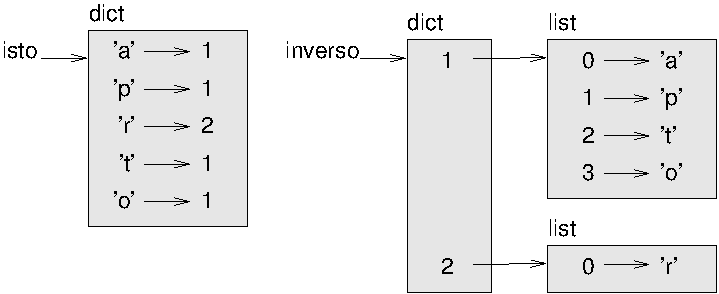
\includegraphics[scale=0.8]{figs/dict1.pdf}}
\caption{Diagramma di stato.}
\label{fig.dict1}
\end{figure}

La Figura~\ref{fig.dict1} è un diagramma di stato che mostra {\tt isto} e {\tt inverso}.
Un dizionario viene rappresentato come un riquadro con la scritta {\tt dict} sopra e le coppie chiave-valore all'interno. Se i valori sono interi, float o stringhe, li raffiguro dentro il riquadro, lascio invece all'esterno le liste per mantenere semplice il diagramma.
\index{diagramma!di stato}

Le liste possono essere valori nel dizionario, come mostra questo esempio, ma non possono essere chiavi. Ecco cosa succede se ci provate:
\index{TypeError}
\index{eccezione!TypeError}


\begin{verbatim}
>>> t = [1, 2, 3]
>>> d = dict()
>>> d[t] = 'oops'
Traceback (most recent call last):
  File "<stdin>", line 1, in ?
TypeError: list objects are unhashable
\end{verbatim}
%
Ho accennato che i dizionari sono implementati usando una tabella hash, e questo implica che alle chiavi deve poter essere applicato un {\bf hash}.
\index{hash, funzione}
\index{hashing}

Un {\bf hash} è una funzione che prende un valore (di qualsiasi tipo) e restituisce un intero. I dizionari usano questi interi, chiamati valori hash, per conservare e consultare le coppie chiave-valore.
\index{immutabilità}

Questo sistema funziona se le chiavi sono immutabili; ma se sono mutabili, come le liste, succedono disastri. Per esempio, nel creare una coppia chiave-valore, Python fa l'hashing della chiave e la immagazzina nello spazio corrispondente. Se modificate la chiave e quindi viene nuovamente calcolato l'hash, si collocherebbe in un altro spazio. In quel caso potreste avere due voci della stessa chiave, oppure non riuscire a trovare una chiave. In ogni caso il dizionario non funzionerà correttamente.

Ecco perché le chiavi devono essere idonee all'hashing, e quelle mutabili come le liste non lo sono. Il modo più semplice per aggirare questo limite è usare le tuple, che vedremo nel prossimo capitolo.

Dato che i dizionari sono mutabili, non possono essere usati come chiavi ma {\em possono} essere usati come valori.


\section{Memoizzazione}
\label{memoize}

Se vi siete sbizzarriti con la funzione {\tt fibonacci} del Paragrafo~\ref{one.more.example}, avrete notato che più grande è l'argomento che passate, maggiore è il tempo necessario per l'esecuzione della funzione. Inoltre, il tempo di elaborazione cresce rapidamente.
\index{fibonacci, funzione}
\index{funzione!fibonacci}

Per capire il motivo, confrontate la Figura~\ref{fig.fibonacci}, che mostra il {\bf grafico di chiamata} di {\tt fibonacci} con {\tt n=4}:

\begin{figure}
\centerline
{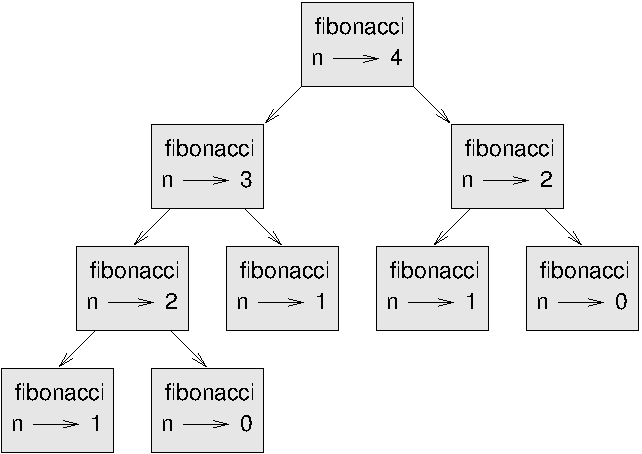
\includegraphics[scale=0.7]{figs/fibonacci.pdf}}
\caption{Grafico di chiamata.}
\label{fig.fibonacci}
\end{figure}

Un grafico di chiamata mostra l'insieme dei frame della funzione, con linee che collegano ciascun frame ai frame delle funzioni che chiama a sua volta. In cima al grafico, {\tt fibonacci} con {\tt n=4} chiama {\tt fibonacci} con {\tt
n=3} e {\tt n=2}.  A sua volta, {\tt fibonacci} con {\tt n=3} chiama
{\tt fibonacci} con {\tt n=2} e {\tt n=1}.  E così via.
\index{funzione!frame di}
\index{frame}
\index{grafico di chiamata}

Provate a contare quante volte vengono chiamate {\tt fibonacci(0)} e {\tt fibonacci(1)}. Questa è una soluzione inefficiente del problema, che peggiora ulteriormente al crescere dell'argomento.
\index{memoizzazione}

Una soluzione migliore è tenere da parte i valori che sono già stati calcolati, conservandoli in un dizionario. La tecnica di conservare per un uso successivo un valore già calcolato, così da non doverlo ricalcolare ogni volta, viene detta {\bf memoizzazione}.  Ecco una versione di {\tt fibonacci} che usa la memoizzazione:

\begin{verbatim}
memo = {0:0, 1:1}

def fibonacci(n):
    if n in memo:
        return memo[n]

    res = fibonacci(n-1) + fibonacci(n-2)
    memo[n] = res
    return res
\end{verbatim}
%
{\tt memo} è un dizionario che conserva i numeri di Fibonacci già conosciuti. Parte con due elementi: 0 che corrisponde a 0, e 1 che corrisponde a 1.

Ogni volta che {\tt fibonacci} viene chiamata, controlla innanzitutto {\tt memo}.
Se quest'ultimo contiene già il risultato, ritorna immediatamente. Altrimenti deve calcolare il nuovo valore, lo aggiunge al dizionario e lo restituisce.

Provate ad eseguire questa versione di {\tt fibonacci} e a confrontarla con l'originale: troverete che è molto più veloce.



\section{Variabili globali}
\index{variabile!globale}

Nell'esempio precedente, {\tt memo} viene creato esternamente alla funzione, pertanto appartiene al frame speciale chiamato \verb"__main__".
Le variabili di \verb"__main__" sono dette anche {\bf globali}
perché ad esse possono accedere tutte le funzioni. A differenza delle variabili locali, che sono distrutte una volta terminata l'esecuzione della loro funzione, quelle globali persistono tra una chiamata di funzione e l'altra.
\index{flag}
\index{main}

Di frequente le variabili globali vengono usate come controlli o {\bf flag}; vale a dire, variabili booleane che indicano quando una certa condizione è soddisfatta (True). Per esempio, alcuni programmi usano un flag di nome {\tt verbose} per controllare che livello di dettaglio dare ad un output:

\begin{verbatim}
verbose = True

def esempio1():
    if verbose:
        print('esempio1 in esecuzione')
\end{verbatim}
%
Se cercate di riassegnare una variabile globale, potreste avere una sorpresa. L'esempio seguente vorrebbe controllare se una funzione è stata chiamata:
\index{riassegnazione}

\begin{verbatim}
stata_chiamata = False

def esempio2():
    stata_chiamata = True         # SBAGLIATO
\end{verbatim}
%
Ma se la eseguite vedrete che il valore di \verb"stata_chiamata"
non cambia. Il motivo è che la funzione {\tt esempio2} crea una nuova variabile di nome \verb"stata_chiamata", che è locale, viene distrutta al termine della funzione e non ha effetti sulla variabile globale.
\index{global, istruzione}
\index{istruzione!global}
\index{dichiarazione}

Per riassegnare una variabile globale dall'interno di una funzione, dovete
{\bf dichiarare} la variabile globale prima di usarla:

\begin{verbatim}
stata_chiamata = False

def esempio2():
    global stata_chiamata 
    stata_chiamata = True
\end{verbatim}
%
L'istruzione {\tt global} dice all'interprete una cosa del genere: ``In questa funzione, quando dico \verb"stata_chiamata", intendo la variabile globale: non crearne una locale''.
\index{aggiornamento!variabile globale}
\index{variabile!globale!aggiornamento}

Ecco un altro esempio che cerca di aggiornare una variabile globale:

\begin{verbatim}
conta = 0

def esempio3():
    conta = conta + 1          # SBAGLIATO
\end{verbatim}
%
Se lo eseguite, ottenete:
\index{UnboundLocalError}
\index{eccezione!UnboundLocalError}

\begin{verbatim}
UnboundLocalError: local variable 'conta' referenced before assignment
\end{verbatim}
%
Python presume che {\tt conta} all'interno della funzione sia una variabile locale, e con questa premessa significa che state usando la variabile prima di averla inizializzata. La soluzione è ancora quella di dichiarare {\tt conta} globale.
\index{contatore}

\begin{verbatim}
def esempio3():
    global conta
    conta += 1
\end{verbatim}
%
Se una variabile globale fa riferimento ad un valore mutabile, potete modificare il valore senza dichiarare la variabile:
\index{mutabilità}

\begin{verbatim}
noto = {0:0, 1:1}

def esempio4():
    noto[2] = 1
\end{verbatim}
%
Pertanto, potete aggiungere, rimuovere e sostituire elementi di una lista o dizionario globali; tuttavia, se volete riassegnare la variabile, occorre dichiararla:

\begin{verbatim}
def esempio5():
    global noto
    noto = dict()
\end{verbatim}
%
Le variabili globali possono risultare utili, ma se ce ne sono molte e le modificate di frequente, possono rendere difficile il debug del programma. 


\section{Debug}
\index{debug}

Se lavorate con banche dati di grosse dimensioni, può diventare oneroso fare il debug stampando e controllando i risultati di output manualmente. Ecco allora alcuni suggerimenti per fare il debug in queste situazioni:

\begin{description}

\item[Ridurre l'input:] Se possibile, riducete le dimensioni della banca dati. Per esempio, se il programma legge un file di testo, cominciate con le sole prime 10 righe o con il più piccolo campione che riuscite a trovare. Potete anche adattare i file stessi, o (meglio) modificare il programma, in modo che legga solo le prime {\tt n} righe.

Se c'è un errore, potete ridurre {\tt n} al più piccolo valore per il quale si manifesta l'errore, poi aumentarlo gradualmente finché non trovate e correggete l'errore.

\item[Controllare riassunti e tipi:] Invece di stampare e controllare l'intera banca dati, prendete in considerazione di stampare riassunti dei dati: ad esempio il numero di elementi in un dizionario o la sommatoria di una lista di numeri.

Una causa frequente di errori in esecuzione è un valore che non è del tipo giusto. Per fare il debug di questo tipo di errori basta spesso stampare il tipo di un valore.

\item[Scrivere controlli automatici:]  Talvolta è utile scrivere del codice per controllare automaticamente gli errori. Per esempio, se dovete calcolare la media di una lista di numeri, potete controllare che il risultato non sia maggiore dell'elemento più grande della lista e non sia minore del più piccolo. Questo è detto ``controllo di congruenza'' perché mira a trovare i risultati ``incongruenti''.
\index{congruenza, controllo di}
\index{coerenza, controllo di}

Un altro tipo di controllo confronta i risultati di due calcoli per vedere se collimano. Questo è chiamato ``controllo di coerenza''.

\item[Stampare gli output in bella copia:] Una buona presentazione dei risultati di debug rende più facile trovare un errore. Abbiamo visto un esempio nel Paragrafo~\ref{factdebug}.  Uno strumento utile è il modulo {\tt pprint}: esso contiene la funzione {\tt pprint} che mostra i tipi predefiniti in un formato più leggibile (pprint infatti sta per ``pretty print'').
\index{bella copia}
\index{pprint, modulo}
\index{modulo!pprint}

\end{description}

Ancora, il tempo che impiegate a scrivere del codice temporaneo può essere ripagato dalla riduzione del tempo di debug.
\index{impalcatura}

\section{Glossario}

\begin{description}

\item[mappatura:] Relazione per cui a ciascun elemento di un insieme corrisponde un elemento di un altro insieme.
\index{mappatura}

\item[dizionario:] Una mappatura da chiavi nei loro valori corrispondenti.
\index{dizionario}

\item[coppia chiave-valore:] Rappresentazione della mappatura da una chiave in un valore.
\index{chiave-valore, coppia}

\item[elemento:] In un dizionario, altro nome della coppia chiave-valore.
\index{elemento!dizionario}

\item[chiave:] Oggetto che compare in un dizionario come prima voce di una coppia chiave-valore.
\index{chiave}

\item[valore:] Oggetto che compare in un dizionario come seconda voce di una coppia chiave-valore. È più specifico dell'utilizzo del termine ``valore'' fatto sinora.
\index{valore}

\item[implementazione:] Un modo per effettuare un'elaborazione.
\index{implementazione}

\item[tabella hash:] Algoritmo usato per implementare i dizionari in Python.
\index{tabella hash}

\item[funzione hash:] Funzione usata da una tabella hash per calcolare la collocazione di una chiave.
\index{hash, funzione}

\item[hash-abile:] Un tipo a cui si può applicare la funzione hash. I tipi immutabili come interi, float e stringhe lo sono; i tipi mutabili come liste e dizionari no.
\index{hashing}

\item[lookup:] Operazione su un dizionario che trova il valore corrispondente a una data chiave.
\index{lookup}

\item[lookup inverso:] Operazione su un dizionario che trova una o più chiavi alle quali è associato un dato valore.
\index{lookup inverso}

\item[singleton:] Lista (o altra sequenza) con un singolo elemento.
\index{singleton}

\item[grafico di chiamata:] Diagramma che mostra tutti i frame creati durante l'esecuzione di un programma, con frecce che collegano ciascun chiamante ad ogni chiamata.
\index{chiamata, grafico di}
\index{diagramma!grafico di chiamata}

\item[memoizzazione:] Conservare un valore calcolato per evitarne il successivo ricalcolo.
\index{memoizzazione}

\item[variabile globale:]  Variabile definita al di fuori di una funzione, alla quale ogni funzione può accedere.
\index{globale, variabile}

\item[istruzione global:]  Istruzione che dichiara globale il nome di una variabile.
\index{global, istruzione}
\index{istruzione!global}

\item[controllo o flag:] Variabile booleana usata per indicare se una condizione è soddisfatta.
\index{flag}

\item[dichiarazione:] Istruzione come {\tt global}, che comunica all'interprete un'informazione su una variabile.
\index{dichiarazione}

\end{description}

\section{Esercizi}


\begin{exercise}
\label{wordlist2}
\index{insieme di appartenenza}
\index{appartenenza!insieme di}

Scrivete una funzione che legga le parole in {\tt words.txt} e le inserisca come chiavi in un dizionario. I valori non hanno importanza. Usate poi l'operatore {\tt in} come modo rapido per controllare se una stringa è contenuta nel dizionario.

Se avete svolto l'Esercizio~\ref{wordlist1}, potete confrontare la velocità di questa implementazione con l'operatore {\tt in} applicato alla lista e la ricerca binaria.

\end{exercise}

\vspace{0.2in}
\begin{exercise}
\label{setdefault}

Leggete la documentazione del metodo dei dizionari {\tt setdefault}
e usatelo per scrivere una versione più concisa di \verb"inverti_diz".
Soluzione: \url{http://thinkpython2.com/code/invert_dict.py}.
\index{setdefault, metodo}
\index{metodo!setdefault}

\end{exercise}

\vspace{0.2in}
\begin{exercise}

Applicate la memoizzazione alla funzione di Ackermann dell'Esercizio~\ref{ackermann} e provate a vedere se questa tecnica rende possibile il calcolo della funzione con argomenti più grandi. Suggerimento: no.
Soluzione: \url{http://thinkpython2.com/code/ackermann_memo.py}.
\index{Ackermann, funzione di}
\index{funzione!ack}

\end{exercise}

\vspace{0.2in}
\begin{exercise}
\index{duplicato}

Se avete svolto l'Esercizio~\ref{duplicate}, avete già una funzione di nome \verb"ha_duplicati" che richiede come parametro una lista e restituisce {\tt True} se ci sono oggetti ripetuti all'interno della lista.

Usate un dizionario per scrivere una versione più rapida e semplice di
\verb"ha_duplicati". 
Soluzione: \url{http://thinkpython2.com/code/has_duplicates.py}.

\end{exercise}

\vspace{0.2in}
\begin{exercise}
\label{exrotatepairs}
\index{lettere!rotazione}
\index{rotazione!lettere}

Due parole sono ``ruotabili'' se potete far ruotare le lettere dell'una per ottenere l'altra (vedere \verb"ruota_parola" nell'Esercizio~\ref{exrotate}).

Scrivete un programma che legga un elenco di parole e trovi tutte le coppie di parole ruotabili. Soluzione: \url{http://thinkpython2.com/code/rotate_pairs.py}.

\end{exercise}

\vspace{0.2in}
\begin{exercise}
\index{Car Talk}
\index{Puzzler}

Ecco un altro quesito tratto da {\em Car Talk} (\url{http://www.cartalk.com/content/puzzlers}):

\begin{quote}
``Questo ci è stato mandato da un amico di nome Dan O'Leary. Si è recentemente imbattuto in una parola inglese di una sillaba e cinque lettere che ha questa singolare proprietà: se togliete la prima lettera, le lettere restanti formano un omofono della prima parola, cioè un'altra parola che pronunciata suona allo stesso modo. Se poi rimettete la prima lettera e togliete la seconda, ottenete ancora un altro omofono della parola di origine. Qual è questa parola?''

``Facciamo un esempio che non funziona del tutto. Prendiamo la parola 'wrack'; togliendo la prima lettera resta 'rack', che è un'altra parola ma è un perfetto omofono. Se però rimettete la prima lettera e togliete la seconda, ottenete 'wack' che pure esiste ma non è un omofono delle altre due parole.''

``Esiste comunque almeno una parola, che Dan e noi conosciamo, che dà due parole omofone di quattro lettere, sia che togliate la prima oppure la seconda lettera.''
\end{quote}
\index{omofono}
\index{riducibile, parola}
\index{parola, riducibile}

Potete usare il dizionario dell'Esercizio~\ref{wordlist2} per controllare se esiste una tale stringa nell'elenco di parole.

Per controllare se due parole sono omofone, potete usare il CMU Pronouncing Dictionary, scaricabile da
\url{http://www.speech.cs.cmu.edu/cgi-bin/cmudict} oppure da
\url{http://thinkpython2.com/code/c06d} e potete anche procurarvi
\url{http://thinkpython2.com/code/pronounce.py}, che fornisce una funzione di nome \verb"read_dictionary" che legge il dizionario delle pronunce e restituisce un dizionario Python in cui a ciascuna parola corrisponde la stringa che ne descrive la pronuncia.

Scrivete un programma che elenchi tutte le parole che risolvono il quesito. Soluzione: \url{http://thinkpython2.com/code/homophone.py}.

\end{exercise}



\chapter{Tuple}
\label{tuplechap}

Questo capitolo illustra un altro tipo di dati predefinito, le tuple, per poi mostrare come liste, tuple e dizionari possono lavorare insieme. Viene inoltre presentata una utile caratteristica per le liste di argomenti a lunghezza variabile: gli operatori di raccolta e spacchettamento.

\section{Le tuple sono immutabili}
\index{tupla}
\index{tipo!tuple}
\index{sequenza}

Una tupla è una sequenza di valori. I valori possono essere di qualsiasi tipo, sono indicizzati tramite numeri interi, e in questo somigliano moltissimo alle liste. La differenza fondamentale è che le tuple sono immutabili.
\index{mutabilità}
\index{immutabilità}

Sintatticamente, la tupla è un elenco di valori separati da virgole:

\begin{verbatim}
>>> t = 'a', 'b', 'c', 'd', 'e'
\end{verbatim}
%
Sebbene non sia necessario, è convenzione racchiudere le tuple tra
   parentesi tonde:
\index{parentesi!tuple in}

\begin{verbatim}
>>> t = ('a', 'b', 'c', 'd', 'e')
\end{verbatim}
%
Per creare una tupla con un singolo elemento, occorre aggiungere una
virgola dopo l'elemento:
\index{singleton}
\index{tupla!singleton}

\begin{verbatim}
>>> t1 = 'a',
>>> type(t1)
<class 'tuple'>
\end{verbatim}
%
Senza la virgola, infatti, un unico valore tra parentesi non è una tupla ma una stringa:

\begin{verbatim}
>>> t2 = ('a')
>>> type(t2)
<class 'str'>
\end{verbatim}
%
Un altro modo di creare una tupla è usare la funzione predefinita {\tt tuple}.
Se priva di argomento, crea una tupla vuota:
\index{tuple, funzione}
\index{funzione!tuple}

\begin{verbatim}
>>> t = tuple()
>>> t
()
\end{verbatim}
%
Se l'argomento è una sequenza (stringa, lista o tupla), il risultato è una tupla con gli elementi della sequenza:

\begin{verbatim}
>>> t = tuple('lupini')
>>> t
('l', 'u', 'p', 'i', 'n', 'i')
\end{verbatim}
%
Siccome {\tt tuple} è il nome di una funzione predefinita, bisogna evitare di usarlo come nome di variabile.

La maggior parte degli operatori delle liste funzionano anche con le tuple. L'operatore parentesi quadre indicizza un elemento della tupla:
\index{parentesi quadre, operatore}
\index{operatore!parentesi quadre}

\begin{verbatim}
>>> t = ('a', 'b', 'c', 'd', 'e')
>>> t[0]
'a'
\end{verbatim}
%
E l'operatore di slicing seleziona una serie di elementi consecutivi:
\index{slicing!operatore di}
\index{operatore!di slicing}
\index{tupla!slicing}
\index{slicing!tupla}

\begin{verbatim}
>>> t[1:3]
('b', 'c')
\end{verbatim}
%
Ma a differenza delle liste, se cercate di modificare gli elementi di una tupla ottenete un messaggio d'errore:
\index{eccezione!TypeError}
\index{TypeError}
\index{elemento!assegnazione}
\index{assegnazione!elemento}

\begin{verbatim}
>>> t[0] = 'A'
TypeError: object doesn't support item assignment
\end{verbatim}
%
Dato che le tuple sono immutabili, non si può modificarne gli elementi. Ma potete sostituire una tupla con un'altra:

\begin{verbatim}
>>> t = ('A',) + t[1:]
>>> t
('A', 'b', 'c', 'd', 'e')
\end{verbatim}
%

Questa istruzione crea una nuova tupla e poi fa in modo che {\tt t} si riferisca ad essa.

Gli operatori di confronto funzionano con le tuple e le altre sequenze; Python inizia a confrontare il primo elemento di ciascuna sequenza. Se sono uguali, passa all'elemento successivo e così via, finché non trova due elementi diversi. Gli eventuali elementi che seguono vengono trascurati (anche se sono molto grandi).

\begin{verbatim}
>>> (0, 1, 2) < (0, 3, 4)
True
>>> (0, 1, 2000000) < (0, 3, 4)
True
\end{verbatim}
%

\section{Assegnazione di tupla}
\label{tuple.assignment}
\index{tupla!assegnazione}
\index{assegnazione!tupla}
\index{scambio, schema di}
\index{schema!di scambio}

Spesso è utile scambiare i valori di due variabili tra loro. Con le istruzioni di assegnazione convenzionali, dobbiamo usare una variabile temporanea. Per esempio per scambiare {\tt a} e {\tt b}:

\begin{verbatim}
>>> temp = a
>>> a = b
>>> b = temp
\end{verbatim}
%
Questo metodo è farraginoso; l'utilizzo dell'{\bf assegnazione di tupla} è più elegante:

\begin{verbatim}
>>> a, b = b, a
\end{verbatim}
%
Sul lato sinistro abbiamo una tupla di variabili; su quello destro, una tupla di espressioni. Ciascun valore viene assegnato alla rispettiva variabile. Tutte le espressioni sul lato destro vengono valutate prima di ogni assegnazione.

Il numero di variabili sulla sinistra deve essere uguale al numero di valori sulla destra:
\index{eccezione!ValueError}
\index{ValueError}

\begin{verbatim}
>>> a, b = 1, 2, 3
ValueError: too many values to unpack
\end{verbatim}
%
Più in generale, sul lato destro può esserci qualsiasi tipo di sequenza (stringhe, liste o tuple). Per esempio, per separare un indirizzo email tra nome utente e dominio, potete scrivere:
\index{split, metodo}
\index{metodo!split}
\index{email, indirizzo}

\begin{verbatim}
>>> indirizzo = 'monty@python.org'
>>> nome, dominio = indirizzo.split('@')
\end{verbatim}
%
Il valore di ritorno del metodo {\tt split} è una lista con due elementi; il primo è assegnato alla variabile {\tt nome}, il secondo a {\tt dominio}.

\begin{verbatim}
>>> nome
'monty'
>>> dominio
'python.org'
\end{verbatim}
%

\section{Tuple come valori di ritorno}
\index{tupla}
\index{valore!tupla}
\index{valore di ritorno!tupla}
\index{funzione!tupla come valore di ritorno}

In senso stretto, una funzione può restituire un solo valore di ritorno, ma se il valore è una tupla, l'effetto pratico è quello di restituire valori molteplici. Per esempio, se volete dividere due interi e calcolare quoziente e resto, è poco efficiente calcolare {\tt x/y} e poi {\tt x\%y}.  Meglio calcolarli entrambi in una volta sola.
\index{divmod}

La funzione predefinita {\tt divmod} riceve due argomenti e restituisce una tupla di due valori, il quoziente e il resto. E potete memorizzare il risultato con una tupla:

\begin{verbatim}
>>> t = divmod(7, 3)
>>> t
(2, 1)
\end{verbatim}
%
Oppure, usate l'assegnazione di tupla per conservare gli elementi separatamente:
\index{tupla!assegnazione}
\index{assegnazione!tupla}

\begin{verbatim}
>>> quoziente, resto = divmod(7, 3)
>>> quoziente
2
>>> resto
1
\end{verbatim}
%
Ecco un esempio di funzione che restituisce una tupla:

\begin{verbatim}
def min_max(t):
    return min(t), max(t)
\end{verbatim}
%
{\tt max} e {\tt min} sono funzioni predefinite che estraggono da una sequenza il valore massimo e quello minimo.  \verb"min_max" li estrae entrambi e restituisce una tupla di due valori.
\index{max, funzione}
\index{funzione!max}
\index{min, funzione}
\index{funzione!min}


\section{Tuple di argomenti a lunghezza variabile}
\label{gather}
\index{lunghezza variabile, tupla di argomenti}
\index{argomento!tupla di lunghezza variabile}
\index{raccolta}
\index{parametro!raccolta}
\index{argomento!raccolta}

Le funzioni possono ricevere un numero variabile di argomenti. Un nome di parametro che comincia con {\tt *}, {\bf raccoglie} gli argomenti in una tupla. Per esempio, {\tt stampatutti} riceve un qualsiasi numero di argomenti e li visualizza:

\begin{verbatim}
def stampatutti(*args):
    print(args)
\end{verbatim}
%
Il parametro di raccolta può avere qualunque nome, ma per convenzione si usa {\tt args}. Ecco come funziona:

\begin{verbatim}
>>> stampatutti(1, 2.0, '3')
(1, 2.0, '3')
\end{verbatim}
%
Il contrario della raccolta è lo {\bf spacchettamento}.  Se avete una sequenza di valori e volete passarla a una funzione come argomenti multipli, usate ancora
 l'operatore {\tt *}. Per esempio, {\tt divmod} richiede esattamente due argomenti; passare una tupla non funziona:
\index{spacchettamento}
\index{argomento!spacchettamento}
\index{TypeError}
\index{eccezione!TypeError}

\begin{verbatim}
>>> t = (7, 3)
>>> divmod(t)
TypeError: divmod expected 2 arguments, got 1
\end{verbatim}
%
Ma se spacchettate la tupla, funziona:

\begin{verbatim}
>>> divmod(*t)
(2, 1)
\end{verbatim}
%


Molte funzioni predefinite possono usare le tuple di argomenti a lunghezza variabile. Ad esempio, {\tt max} e {\tt min} ricevono un numero qualunque di argomenti:
\index{max, funzione}
\index{funzione!max}
\index{min, funzione}
\index{funzione!min}

\begin{verbatim}
>>> max(1,2,3)
3
\end{verbatim}
%
Ma con {\tt sum} non funziona.
\index{sum, funzione}
\index{funzione!sum}

\begin{verbatim}
>>> sum(1,2,3)
TypeError: sum expected at most 2 arguments, got 3
\end{verbatim}
%
Per esercizio, scrivete una funzione di nome {\tt sommatutto} che riceva un numero di argomenti a piacere e ne restituisca la somma.


\section{Liste e tuple}
\index{zip, funzione}
\index{funzione!zip}

{\tt zip} è una funzione predefinita che riceve due o più sequenze e restituisce una lista di tuple, dove ciascuna tupla contiene un elemento di ciascuna sequenza.  Il nome si riferisce alla cerniera-lampo ({\em zipper}), che unisce due file di dentelli, alternandoli.

Questo esempio abbina una stringa e una lista:

\begin{verbatim}
>>> s = 'abc'
>>> t = [0, 1, 2]
>>> zip(s, t)
<zip object at 0x7f7d0a9e7c48>
\end{verbatim}
%

Il risultato è un {\bf oggetto zip} capace di iterare attraverso le coppie.  L'uso più frequente di {\tt zip} è in un ciclo {\tt for}:

\begin{verbatim}
>>> for coppia in zip(s, t):
...     print(coppia)
...
('a', 0)
('b', 1)
('c', 2)
\end{verbatim}
%
Un oggetto zip è un tipo di {\bf iteratore}, che è un qualsiasi oggetto in grado di iterare attraverso una sequenza. Gli iteratori sono per certi versi simili alle liste, ma a differenza di queste ultime, non si può usare un indice per scegliere un elemento da un iteratore.
\index{iteratore}

Se desiderate usare operatori e metodi delle liste, potete crearne una utilizzando un oggetto zip:

\begin{verbatim}
>>> list(zip(s, t))
[('a', 0), ('b', 1), ('c', 2)]
\end{verbatim}
%
Il risultato è una lista di tuple, e in questo esempio ciascuna tupla contiene un carattere della stringa e il corrispondente elemento della lista.
\index{lista!di tuple}

Se le sequenze non sono della stessa lunghezza, il risultato ha la lunghezza di quella più corta:

\begin{verbatim}
>>> list(zip('Anna', 'Edo'))
[('A', 'E'), ('n', 'd'), ('n', 'o')]
\end{verbatim}
%
Potete usare l'assegnazione di tupla in un ciclo {\tt for} per attraversare una lista di tuple:
\index{attraversamento}
\index{tupla!assegnazione}
\index{assegnazione!tupla}

\begin{verbatim}
t = [('a', 0), ('b', 1), ('c', 2)]
for lettera, numero in t:
    print(numero, lettera)
\end{verbatim}
%
Ad ogni ciclo, Python seleziona la tupla successiva all'interno della lista e ne assegna gli elementi a {\tt lettera} e {\tt numero}, quindi li stampa.  Il risultato di questo ciclo è:
\index{ciclo}

\begin{verbatim}
0 a
1 b
2 c
\end{verbatim}
%
Se combinate {\tt zip}, {\tt for} e assegnazione di tupla, ottenete un utile costrutto per attraversare due o più sequenze contemporaneamente. Per esempio, \verb"corrispondenza" prende due sequenze, {\tt t1} e
{\tt t2}, e restituisce {\tt True} se esiste almeno un indice {\tt i}
tale che {\tt t1[i] == t2[i]}:
\index{for, ciclo}

\begin{verbatim}
def corrispondenza(t1, t2):
    for x, y in zip(t1, t2):
        if x == y:
            return True
    return False
\end{verbatim}
%
Se volete attraversare gli elementi di una sequenza e i loro indici, potete usare la funzione predefinita {\tt enumerate}:
\index{attraversamento}
\index{enumerate, funzione}
\index{funzione!enumerate}

\begin{verbatim}
for indice, elemento in enumerate('abc'):
    print(indice, elemento)
\end{verbatim}
%
Il risultato di {\tt enumerate} è un oggetto enumerate, che itera una sequenza di coppie; ogni coppia contiene un indice (a partire da 0) e un elemento della sequenza data.
In questo esempio l'output è di nuovo:

\begin{verbatim}
0 a
1 b
2 c
\end{verbatim}
%
\index{iteratore}
\index{oggetto!enumerate}
\index{enumerate, oggetto}
%


\section{Dizionari e tuple}
\label{dictuple}
\index{dizionario}
\index{items, metodo}
\index{metodo!items}
\index{chiave-valore, coppia}

I dizionari supportano un metodo di nome {\tt items} che restituisce una sequenza di tuple, dove ogni tupla è una delle coppie chiave-valore.

\begin{verbatim}
>>> d = {'a':0, 'b':1, 'c':2}
>>> t = d.items()
>>> t
dict_items([('c', 2), ('a', 0), ('b', 1)])
\end{verbatim}
%
Il risultato è un oggetto \verb"dict_items", un iteratore che itera le coppie chiave-valore. Si può usare in un ciclo {\tt for} in questo modo:
\index{iteratore}

\begin{verbatim}
>>> for chiave, valore in d.items():
...     print(chiave, valore)
...
c 2
a 0
b 1
\end{verbatim}

Come di consueto per i dizionari, gli elementi non sono in un ordine particolare.
Per altro verso, potete usare una lista di tuple per inizializzare un nuovo dizionario: \index{dizionario!inizializzazione}

\begin{verbatim}
>>> t = [('a', 0), ('c', 2), ('b', 1)]
>>> d = dict(t)
>>> d
{'a': 0, 'c': 2, 'b': 1}
\end{verbatim}

La combinazione di {\tt dict} e {\tt zip} produce un modo conciso di creare un dizionario:
\index{zip, funzione!uso con dict}

\begin{verbatim}
>>> d = dict(zip('abc', range(3)))
>>> d
{'a': 0, 'c': 2, 'b': 1}
\end{verbatim}
%
Anche il metodo dei dizionari {\tt update} prende una lista di tuple e le aggiunge, come coppie chiave-valore, a un dizionario esistente.
\index{update, metodo}
\index{metodo!update}
\index{attraversamento!dizionario}
\index{dizionario!attraversamento}

L'uso delle tuple come chiavi di un dizionario è frequente (soprattutto perché le liste non si possono usare in quanto mutabili). Per esempio, un elenco telefonico può mappare da coppie di nomi e cognomi nei numeri di telefono. Supponendo di aver definito {\tt cognome}, {\tt nome} e {\tt numero}, possiamo scrivere:
\index{tupla!come chiave di dizionario}
\index{hashing}

\begin{verbatim}
elenco[cognome,nome] = numero
\end{verbatim}
%
L'espressione tra parentesi quadre è una tupla. Possiamo usare l'assegnazione di tupla per attraversare questo dizionario.
\index{tupla!in parentesi quadre}

\begin{verbatim}
for cognome, nome in elenco:
    print(nome, cognome, elenco[cognome,nome])
\end{verbatim}
%
Questo ciclo attraversa le chiavi in {\tt elenco}, che sono tuple. Assegna gli elementi di ogni tupla a {\tt cognome} e {\tt nome}, quindi stampa il nome completo e il numero di telefono corrispondente.

Ci sono due modi per rappresentare le tuple in un diagramma di stato. La versione più dettagliata mostra gli indici e gli elementi così come compaiono in una lista. Per esempio la tupla \verb"('Cleese', 'John')" comparirebbe come in Figura~\ref{fig.tuple1}.
\index{diagramma!di stato}

\begin{figure}
\centerline
{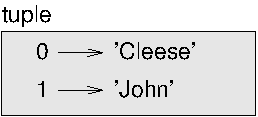
\includegraphics[scale=0.8]{figs/tuple1.pdf}}
\caption{Diagramma di stato.}
\label{fig.tuple1}
\end{figure}

Ma in un diagramma più ampio è meglio tralasciare i dettagli. Per esempio, quello dell'elenco telefonico può essere come in Figura~\ref{fig.dict2}.

\begin{figure}
\centerline
{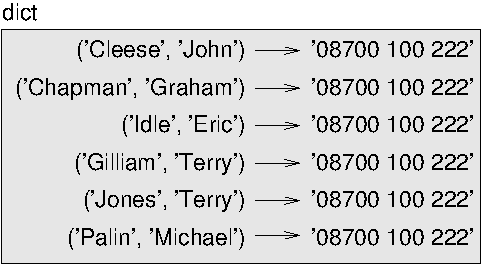
\includegraphics[scale=0.8]{figs/dict2.pdf}}
\caption{Diagramma di stato.}
\label{fig.dict2}
\end{figure}

Qui le tuple sono mostrate usando la sintassi di Python come abbreviazione grafica. Il numero di telefono nel diagramma è quello dei reclami della BBC, per cui vi prego, non chiamatelo.


\section{Sequenze di sequenze}
\index{sequenza}

Ci siamo concentrati finora sulle liste di tuple, ma quasi tutti gli esempi di questo capitolo funzionano anche con liste di liste, tuple di tuple, e tuple di liste. Per evitare di elencare tutte le possibili combinazioni, è più semplice usare il termine sequenze di sequenze.

In molti casi, i diversi tipi di sequenze (strighe, liste, tuple) possono essere intercambiabili. E allora, con che criterio usarne una piuttosto di un'altra?
\index{stringa}
\index{lista}
\index{tupla}
\index{mutabilità}
\index{immutabilità}

Le stringhe sono ovviamente le più limitate, perché gli elementi devono essere dei caratteri. E sono anche immutabili. Se dovete cambiare i caratteri in una stringa, anziché crearne una nuova, utilizzare una lista di caratteri può essere una scelta migliore.

Le liste sono usate più di frequente delle tuple, soprattutto perché sono mutabili. Ma ci sono alcuni casi in cui le tuple sono preferibili:

\begin{enumerate}

\item In certi contesti, come un'istruzione {\tt return}, è sintatticamente più semplice creare una tupla anziché una lista.

\item Se vi serve una sequenza da usare come chiave di un dizionario, dovete per forza usare un tipo immutabile come una tupla o una stringa.

\item Se state passando una sequenza come argomento a una funzione, usare le tuple riduce le possibilità di comportamenti imprevisti dovuti agli alias.

\end{enumerate}

Siccome le tuple sono immutabili, non possiedono metodi come {\tt sort} e {\tt reverse}, che modificano delle liste esistenti.
Però Python contiene la funzione {\tt sorted}, che richiede una sequenza e restituisce una nuova lista con gli stessi elementi della sequenza, ordinati, e {\tt reversed}, che prende una sequenza e restituisce un iteratore che attraversa la lista in ordine inverso.
\index{sorted, funzione}
\index{funzione!sorted}
\index{reversed, funzione}
\index{funzione!reversed}
\index{iteratore}


\section{Debug}
\index{debug}
\index{struttura di dati}
\index{formato, errore di}
\index{errore!di formato}

Liste, dizionari e tuple sono esempi di {\bf strutture di dati}; in questo capitolo abbiamo iniziato a vedere strutture di dati composte, come liste di tuple, o dizionari che contengono tuple come chiavi e liste come valori. Si tratta di elementi utili, ma soggetti a quelli che io chiamo {\tt errori di formato}; cioè errori causati dal fatto che una struttura di dati è di tipo, dimensione o struttura sbagliati. Ad esempio, se un programma si aspetta una lista che contiene un numero intero e invece gli passate un intero puro e semplice (non incluso in una lista), non funzionerà.
\index{structshape, modulo}
\index{modulo!structshape}

Per facilitare il debug di questo genere di errori, ho scritto un modulo di nome {\tt structshape} che contiene una funzione, anch'essa di nome
{\tt structshape}, che riceve come argomento una qualunque struttura di dati e restituisce una stringa che ne riassume il formato. Potete scaricarlo dal sito \url{http://thinkpython2.com/code/structshape.py}

Questo è il risultato per una lista semplice:

\begin{verbatim}
>>> from structshape import structshape
>>> t = [1,2,3]
>>> structshape(t)
'list of 3 int'
\end{verbatim}
%
Un programma più aggraziato avrebbe scritto ``list of 3 int{\em s}'', ma è più semplice non avere a che fare con i plurali. Ecco una lista di liste:

\begin{verbatim}
>>> t2 = [[1,2], [3,4], [5,6]]
>>> structshape(t2)
'list of 3 list of 2 int'
\end{verbatim}
%
Se gli elementi della lista non sono dello stesso tipo,
{\tt structshape} li raggruppa, in ordine, per tipo:

\begin{verbatim}
>>> t3 = [1, 2, 3, 4.0, '5', '6', [7], [8], 9]
>>> structshape(t3)
'list of (3 int, float, 2 str, 2 list of int, int)'
\end{verbatim}
%
Ecco una lista di tuple:

\begin{verbatim}
>>> s = 'abc'
>>> lt = zip(list(t, s))
>>> structshape(lt)
'list of 3 tuple of (int, str)'
\end{verbatim}
%
Ed ecco un dizionario di 3 elementi in cui corrispondono interi a stringhe

\begin{verbatim}
>>> d = dict(lt) 
>>> structshape(d)
'dict of 3 int->str'
\end{verbatim}
%
Se fate fatica a tenere sotto controllo le vostre strutture di dati,
{\tt structshape} può esservi di aiuto.


\section{Glossario}

\begin{description}

\item[tupla:] Una sequenza di elementi immutabile.
\index{tupla}

\item[assegnazione di tupla:] Assegnazione costituita da una sequenza sul lato destro e una tupla di variabili su quello sinistro. Il lato destro viene valutato, quindi gli elementi vengono assegnati alle variabili sulla sinistra.
\index{tupla!assegnazione}
\index{assegnazione!tupla}

\item[raccolta:] L'operazione di assemblare una tupla di argomenti a lunghezza variabile.
\index{raccolta}

\item[spacchettamento:] L'operazione di trattare una sequenza come una lista di argomenti.
\index{spacchettamento}

\item[oggetto zip:] Il risultato della chiamata della funzione predefinita {\tt zip}; un oggetto che itera attraverso una sequenza di tuple.
\index{zip, oggetto}
\index{oggetto!zip}

\item[iteratore:] Un oggetto in grado di iterare attraverso una sequenza, ma che non fornisce operatori e metodi delle liste.
\index{iteratore}

\item[struttura di dati:] Una raccolta di valori correlati, spesso organizzati in liste, dizionari, tuple, ecc.
\index{struttura di dati}

\item[errore di formato:] Errore dovuto ad un valore che ha un formato sbagliato, ovvero tipo o dimensioni errati.
\index{formato}

\end{description}


\section{Esercizi}

\begin{exercise}

Scrivete una funzione di nome \verb"piu_frequente" che riceva una stringa e stampi le lettere in ordine di frequenza decrescente. Trovate delle frasi di esempio in diverse lingue e osservate come varia la frequenza delle lettere. Confrontate i vostri risultati con le tabelle del sito
\url{http://en.wikipedia.org/wiki/Letter_frequencies}.  Soluzione:
\url{http://thinkpython2.com/code/most_frequent.py}.  
\index{lettere!frequenza} 
\index{frequenza!di lettere}

\end{exercise}

\vspace{0.2in}
\begin{exercise}
\label{anagrams}
\index{anagramma, insieme}
\index{insieme!anagramma}

Ancora anagrammi!

\begin{enumerate}

\item Scrivete un programma che legga un elenco di parole da un file (vedi Paragrafo~\ref{wordlist}) e stampi tutti gli insiemi di parole che sono tra loro anagrammabili.

Un esempio di come si può presentare il risultato:

\begin{verbatim}
['deltas', 'desalt', 'lasted', 'salted', 'slated', 'staled']
['retainers', 'ternaries']
['generating', 'greatening']
['resmelts', 'smelters', 'termless']
\end{verbatim}
%
Suggerimento: potete costruire un dizionario che faccia corrispondere un gruppo di lettere con una lista di parole che si possono scrivere con quelle lettere. Il problema è: come rappresentare il gruppo di lettere in modo che possano essere usate come chiave?

\item Modificate il programma in modo che stampi la lista di anagrammi più lunga per prima, seguita dalla seconda più lunga, e così via.
\index{Scarabeo}

\item Nel gioco da tavolo {\em Scarabeo}, fate un ``en-plein'' quando giocate tutte le sette lettere sul vostro leggio formando, insieme a una lettera sul tavolo, una parola di otto lettere. Con quale gruppo di 8 lettere si può fare un ``en-plein'' con maggior probabilità?
Suggerimento: il gruppo dà sette combinazioni.

% (7, ['angriest', 'astringe', 'ganister', 'gantries', 'granites',
% 'ingrates', 'rangiest'])

Soluzione: \url{http://thinkpython2.com/code/anagram_sets.py}.

\end{enumerate}
\end{exercise}

\vspace{0.2in}
\begin{exercise}
\index{metatesi}

Si ha una metatesi quando una parola si può ottenere scambiando due lettere di un'altra parola, per esempio: ``conversa'' e ``conserva''.  Scrivete un programma che trovi tutte le coppie con metatesi nel dizionario. Suggerimento: non provate tutte le possibili coppie di parole e non provate tutti i possibili scambi. Soluzione: \url{http://thinkpython2.com/code/metathesis.py}.
Fonte: Esercizio suggerito da un esempio nel sito \url{http://puzzlers.org}.

\end{exercise}


\vspace{0.2in}
\begin{exercise}
\index{Car Talk}
\index{Puzzler}

Ed ecco un altro quesito di Car Talk:
(\url{http://www.cartalk.com/content/puzzlers}):

\begin{quote}
Qual è la più lunga parola inglese che rimane una parola valida se le togliete una lettera alla volta? 
Le lettere possono essere rimosse sia agli estremi o in mezzo, ma senza spostare le lettere rimanenti. Ogni volta che togliete una lettera, ottenete un'altra parola inglese. Se andate avanti, ottenete un'altra parola. Ora, voglio sapere qual è la parola più lunga possibile e quante lettere ha.

Vi faccio un piccolo esempio: Sprite. Partite da sprite, togliete una lettera, una interna, come la r e resta la parola spite, poi togliete la e finale e avete spit, togliamo la s e resta pit, poi it, infine I.
\end{quote}
\index{parola, riducibile}

Scrivete un programma che trovi tutte le parole che sono riducibili in questa maniera, quindi trovate la più lunga.

Questo esercizio è un po' più impegnativo degli altri, quindi eccovi alcuni suggerimenti:

\begin{enumerate}

\item Potete scrivere una funzione che prenda una parola e calcoli una lista di tutte le parole che si possono formare togliendo una lettera. Queste sono le ``figlie'' della parola.
\index{definizione!ricorsiva}

\item Ricorsivamente, una parola è riducibile se qualcuna delle sue figlie è a sua volta riducibile. Come caso base, potete considerare riducibile la stringa vuota.

\item L'elenco di parole che ho fornito, {\tt words.txt}, non contiene parole di una lettera. Potete quindi aggiungere ``I'', ``a'', e la stringa vuota.

\item Per migliorare le prestazioni del programma, potete memoizzare le parole che sono risultate riducibili.

\end{enumerate}

Soluzione: \url{http://thinkpython2.com/code/reducible.py}.

\end{exercise}



\chapter{Esercitazione: Scelta della struttura di dati}

Giunti a questo punto, avete conosciuto le principali strutture di dati di Python, e avete visto alcuni algoritmi che le utilizzano. Se vi interessa saperne di più sugli algoritmi, potrebbe essere un buon momento per leggere l'Appendice~\ref{algorithms}.
Non è però necessario per proseguire la lettura: fatelo quando vi pare opportuno.

L'esercitazione di questo capitolo vi aiutèrà ad impratichirvi nella scelta e nell'uso delle strutture di dati.

\section{Analisi di frequenza delle parole}
\label{analysis}

Come al solito, tentate almeno di risolvere gli esercizi prima di guardare le mie risoluzioni.

\vspace{0.2in}
\begin{exercise}

Scrivete un programma che legga un file di testo, separi da ogni riga le singole parole, scarti gli spazi bianchi e la punteggiatura dalle parole, e converta tutto in lettere minuscole.
\index{string, modulo}
\index{modulo!string}

Suggerimento: il modulo {\tt string} fornisce una stringa chiamata {\tt whitespace}, che contiene i caratteri spaziatori come spazio, tabulazione, a capo ecc., e una di nome {\tt punctuation} che contiene i caratteri di punteggiatura. Vediamo se Python ce lo conferma:

\begin{verbatim}
>>> import string
>>> string.punctuation
'!"#$%&'()*+,-./:;<=>?@[\]^_`{|}~'
\end{verbatim}
%
Potete anche fare uso dei metodi delle stringhe {\tt strip},
{\tt replace} e {\tt translate}.
\index{strip, metodo}
\index{metodo!strip}
\index{replace, metodo}
\index{metodo!replace}
\index{translate, metodo}
\index{metodo!translate}

\end{exercise}

\vspace{0.2in}
\begin{exercise}
\index{Progetto Gutenberg}

Andate sul sito del Progetto Gutenberg (\url{http://gutenberg.org}) e scaricate il libro fuori copyright che preferite, in formato di testo semplice.
\index{testo!semplice}

Modificate il programma dell'esercizio precedente in modo che legga il libro da voi scaricato, salti le informazioni di intestazione all'inizio del file, ed elabori il resto come sopra.

Quindi modificate il programma in modo che conti il numero di parole totale del libro, e quante volte è usata ciascuna parola.
\index{parola, frequenza}
\index{frequenza!di parole}

Visualizzate il numero di parole diverse usate nel libro. Confrontate libri diversi di diversi autori, scritti in epoche diverse. Quale autore usa il vocabolario più ricco?
\end{exercise}

\vspace{0.2in}
\begin{exercise}

Modificate il programma dell'esercizio precedente in modo da visualizzare le 20 parole più usate nel libro.

\end{exercise}

\vspace{0.2in}
\begin{exercise}

Modificate il programma precedente in modo che acquisisca un elenco di parole (vedi Paragrafo~\ref{wordlist}) e quindi stampi l'elenco delle parole contenute nel libro che non sono presenti nell'elenco di parole. Quante di esse sono errori di stampa? Quante sono parole comuni che {\em dovrebbero} essere nell'elenco, e quante sono del tutto oscure?

\end{exercise}


\section{Numeri casuali}
\index{numero casuale}
\index{deterministico}
\index{pseudocasuale}

A parità di dati in ingresso, la maggior parte dei programmi genera gli stessi risultati ad ogni esecuzione, e per questo motivo sono detti deterministici. Di solito il determinismo è una cosa giusta, poiché è ovvio attendersi che gli stessi dati producano gli stessi risultati. Per certe applicazioni, tuttavia, è richiesto che l'elaboratore sia imprevedibile: i videogiochi sono un classico esempio, ma ce ne sono anche altri.

Creare un programma realmente non-deterministico è una cosa piuttosto difficile, ma ci sono dei sistemi per renderlo almeno apparentemente non-deterministico. Uno di questi è utilizzare degli algoritmi che generano dei numeri {\bf pseudocasuali}. Questi numeri non sono veri numeri casuali, dato che sono generati da un elaboratore deterministico, ma a prima vista è praticamente impossibile distinguerli da numeri casuali.
\index{random, modulo}
\index{modulo!random}

Il modulo {\tt random} contiene delle funzioni che generano numeri pseudocasuali (d'ora in avanti chiamati ``casuali'' per semplicità).
\index{random, funzione}
\index{funzione!random}

La funzione {\tt random} restituisce un numero casuale in virgola mobile compreso nell'intervallo tra 0.0 e 1.0 (incluso 0.0 ma escluso 1.0).  Ad ogni chiamata di {\tt random}, si ottiene il numero successivo di una lunga serie di numeri casuali. Per vedere un esempio provate ad eseguire questo ciclo:

\begin{verbatim}
import random

for i in range(10):
    x = random.random()
    print(x)
\end{verbatim}
%
La funzione {\tt randint} richiede due parametri interi, uno  {\tt inferiore} e uno  {\tt superiore}, e restituisce un intero casuale nell'intervallo tra i due parametri (entrambi compresi)
\index{randint, funzione}
\index{funzione!randint}

\begin{verbatim}
>>> random.randint(5, 10)
5
>>> random.randint(5, 10)
9
\end{verbatim}
%
Per estrarre un elemento a caso da una sequenza, potete usare
{\tt choice}:
\index{choice, funzione}
\index{funzione!choice}

\begin{verbatim}
>>> t = [1, 2, 3]
>>> random.choice(t)
2
>>> random.choice(t)
3
\end{verbatim}
%
Il modulo {\tt random} contiene anche delle funzioni per generare valori pseudocasuali da distribuzioni continue, incluse gaussiane, esponenziali, gamma, e alcune altre.

\vspace{0.2in}
\begin{exercise}
\index{istogramma!scelta casuale}

Scrivete una funzione di nome \verb"estrai_da_isto" che prenda un istogramma come definito nel Paragrafo~\ref{histogram} e restituisca un valore casuale dall'istogramma, scelto in modo che la probabilità sia proporzionale alla frequenza. Per esempio, dato questo istogramma:

\begin{verbatim}
>>> t = ['a', 'a', 'b']
>>> isto = istogramma(t)
>>> isto
{'a': 2, 'b': 1}
\end{verbatim}
%
la vostra funzione dovrebbe restituire \verb"'a'" con probabilità $2/3$ e \verb"'b'" con probabilità $1/3$.
\end{exercise}


\section{Istogramma di parole}

Provate a risolvere gli esercizi precedenti prima di procedere oltre. Le soluzioni sono scaricabili da
 \url{http://thinkpython2.com/code/analyze_book1.py}.  Vi servirà anche \url{http://thinkpython2.com/code/emma.txt}.

Ecco un programma che legge un file e costruisce un istogramma della parole in esso contenute:
\index{istogramma!frequenza delle parole}

\begin{verbatim}
import string

def elabora_file(nomefile):
    isto = dict()
    fp = open(nomefile)
    for riga in fp:
        elabora_riga(riga, isto)
    return isto

def elabora_riga(riga, isto):
    riga = riga.replace('-', ' ')
    
    for parola in riga.split():
        parola = parola.strip(string.punctuation + string.whitespace)
        parola = parola.lower()
        isto[parola] = isto.get(parola, 0) + 1

isto = elabora_file('emma.txt')
\end{verbatim}
%
Questo programma legge il file {\tt emma.txt}, che contiene il testo di {\em
  Emma} di Jane Austen.
\index{Austin, Jane}

\verb"elabora_file" legge ciclicamente le righe del file, passandole una per volta a \verb"elabora_riga".  L'istogramma {\tt isto} viene usato come un accumulatore.
\index{accumulatore!istogramma}
\index{attraversamento}

\verb"elabora_riga" usa il metodo delle stringhe {\tt replace} per sostituire i trattini con gli spazi, prima di usare {\tt split} per suddividere la riga in una lista di stringhe. Attraversa poi la lista di parole e usa {\tt strip}
e {\tt lower} per togliere la punteggiatura e convertire in lettere minuscole. (Diciamo per semplicità che le stringhe sono ``convertite'': essendo queste immutabili, i metodi come {\tt strip} e {\tt lower} in realtà restituiscono nuove stringhe).

Infine, \verb"elabora_riga" aggiorna l'istogramma creando un nuovo elemento o incrementandone uno esistente.
\index{aggiornamento!istogramma}

Per contare il numero di parole totali, possiamo aggiungere le frequenze nell'istogramma:

\begin{verbatim}
def parole_totali(isto):
    return sum(isto.values())
\end{verbatim}
%
Il numero di parole diverse è semplicemente il numero di elementi nel dizionario:

\begin{verbatim}
def parole_diverse(isto):
    return len(isto)
\end{verbatim}
%
Ed ecco del codice per stampare i risultati:

\begin{verbatim}
print('Numero totale di parole:', parole_totali(isto))
print('Numero di parole diverse:', parole_diverse(isto))
\end{verbatim}
%
E i relativi risultati:

\begin{verbatim}
Numero totale di parole: 161080
Numero di parole diverse: 7214
\end{verbatim}
%

\section{Parole più comuni}

Per trovare le parole più comuni, possiamo creare una lista di tuple, in cui ciascuna tupla contiene una parola e la sua frequenza, ed ordinarle:

La  funzione seguente prende un istogramma e restituisce una lista di tuple parola-frequenza:

\begin{verbatim}
def piu_comuni(isto):
    t = []
    for chiave, valore in isto.items():
        t.append((valore, chiave))

    t.sort(reverse=True)
    return t
\end{verbatim}
%
In ogni tupla, la frequenza compare per prima, quindi la lista risultante è ordinata per frequenza. Ecco un ciclo che stampa le dieci parole più comuni:

\begin{verbatim}
t = piu_comuni(hist)
print('Le parole più comuni sono:')
for freq, parola in t[:10]:
    print(parola, freq, sep='\t')
\end{verbatim}
%
Ho usato l'argomento con nome {\tt sep} per dire a {\tt print} di usare un carattere di tabulazione come ``separatore'', anziché uno spazio, in modo che la seconda colonna risulti allineata.
E questi sono i risultati nel caso di {\em Emma}:

\begin{verbatim}
Le parole più comuni sono:
to      5242
the     5205
and     4897
of      4295
i       3191
a       3130
it      2529
her     2483
was     2400
she     2364
\end{verbatim}
%
Si potrebbe semplificare il codice utilizzando il parametro {\tt key} della funzione {\tt sort}.  Se vi incuriosisce, leggete
\url{https://wiki.python.org/moin/HowTo/Sorting}.

\section{Parametri opzionali}
\index{parametro!opzionale}

Abbiamo già visto funzioni predefinite e metodi che ricevono argomenti opzionali. È possibile anche scrivere funzioni personalizzate con degli argomenti opzionali. Ad esempio, questa è una funzione che stampa le parole più comuni in un istogramma:
\index{funzione!personalizzata}

\begin{verbatim}
def stampa_piu_comuni(isto, num=10):
    t = piu_comuni(isto)
    print('Le parole più comuni sono:')
    for freq, parola in t[:num]:
        print(parola, freq, sep='\t')
\end{verbatim}

Il primo parametro è obbligatorio; il secondo è opzionale. Il {\bf valore di default} di {\tt num} è 10.
\index{valore di default}

Se passate un solo argomento:

\begin{verbatim}
stampa_piu_comuni(isto)
\end{verbatim}

{\tt num} assume il valore predefinito. Se ne passate due:

\begin{verbatim}
stampa_piu_comuni(isto, 20)
\end{verbatim}

{\tt num} assume il valore che avete specificato. In altre parole, l'argomento opzionale {\bf sovrascrive} il valore predefinito.
\index{sovrascrittura}

Se una funzione ha sia parametri obbligatori che opzionali, tutti quelli obbligatori devono essere scritti per primi, seguiti da quelli opzionali.


\section{Sottrazione di dizionari}
\label{dictsub}
\index{dizionario!sottrazione}
\index{sottrazione!dizionario}

Trovare le parole del libro non comprese nell'elenco {\tt words.txt} è un problema che possiamo classificare come sottrazione di insiemi, cioè occorre trovare le parole appartenenti a un insieme (le parole contenute nel libro) che non si trovano nell'altro insieme (l'elenco).

{\tt sottrai} prende i dizionari {\tt d1} e {\tt d2} e ne restituisce uno nuovo che contiene tutte le chiavi di {\tt d1} che non si trovano in {\tt d2}.  Siccome non ci interessano affatto i valori, li impostiamo tutti a None.

\begin{verbatim}
def sottrai(d1, d2):
    res = dict()
    for chiave in d1:
        if chiave not in d2:
            res[chiave] = None
    return res
\end{verbatim}
%
Quindi usiamo \verb"elabora_file" per costruire un istogramma di
{\tt words.txt}, per poi sottrarre:

\begin{verbatim}
parole = elabora_file('words.txt')
diff = sottrai(isto, parole)

print('Parole del libro che non si trovano nell'elenco:')
for parola in diff:
    print(parola, end=' ')
\end{verbatim}
%
Ecco alcuni risultati per {\em Emma}:

\begin{verbatim}
Parole del libro che non si trovano nell'elenco:
 rencontre jane's blanche woodhouses disingenuousness 
friend's venice apartment ...
\end{verbatim}
%
Alcune parole sono nomi propri e possessivi. Altre come ``rencontre'' sono desuete. Ma qualcuna è davvero una parola comune che nell'elenco dovrebbe esserci!

\vspace{0.2in}
\begin{exercise}
\index{insieme}
\index{tipo!set}

Python dispone di una struttura di dati chiamata {\tt set}, o insieme, che fornisce molte operazioni comuni sugli insiemi. Al riguardo, potete leggere il Paragrafo~\ref{sets} o la documentazione sul sito  
\url{http://docs.python.org/3/library/stdtypes.html#types-set}. 

Scrivete un programma che usi la sottrazione di insiemi per trovare le parole del libro che non sono nell'elenco. Soluzione:
\url{http://thinkpython2.com/code/analyze_book2.py}.

\end{exercise}


\section{Parole a caso}
\label{randomwords}
\index{istogramma!scelta casuale}

Per scegliere una parola a caso dall'istogramma, l'algoritmo più semplice è  costruire una lista che contiene più copie di ciascuna parola, secondo la frequenza osservata, e poi estrarre a caso da questa lista:

\begin{verbatim}
def parola_caso(h):
    t = []
    for parola, freq in h.items():
        t.extend([parola] * freq)

    return random.choice(t)
\end{verbatim}
%
L'espressione {\tt [parola] * freq} crea una lista con {\tt freq}
copie della stringa {\tt parola}.  Il metodo {\tt extend}
è simile a {\tt append}, con la differenza che l'argomento è una sequenza.

Questo algoritmo funziona, ma non è molto efficiente: ogni volta che estraete una parola, ricostruisce la lista, che è grande come il libro originale. Un ovvio miglioramento è di costruire la lista una sola volta e poi fare estrazioni multiple, ma la lista è ancora grande.

Un'alternativa è:

\begin{enumerate}

\item Usare {\tt keys} per ottenere una lista delle parole del libro.

\item Costruire una lista che contiene la somma cumulativa delle frequenze delle parole (vedere l'Esercizio~\ref{cumulative}).  L'ultimo elemento della lista è il numero totale delle parole nel libro, $n$.
  
\item Scegliere un numero a caso da 1 a $n$.  Usare una ricerca binaria
  (vedere l'Esercizio~\ref{bisection}) per trovare l'indice dove il numero casuale si inserirebbe nella somma cumulativa.

\item Usare l'indice per trovare la parola corrispondente nella lista di parole.

\end{enumerate}

\vspace{0.2in}
\begin{exercise}
\label{randhist}
\index{algoritmo}

Scrivete un programma che usi questo algoritmo per scegliere una parola a caso dal libro. Soluzione: \url{http://thinkpython2.com/code/analyze_book3.py}.

\end{exercise}



\section{Analisi di Markov}
\label{markov}
\index{Markov, analisi di}

Scegliendo a caso delle parole dal libro, potete avere un'idea del vocabolario usato dall'autore, ma difficilmente otterrete una frase di senso compiuto:

\begin{verbatim}
this the small regard harriet which knightley's it most things
\end{verbatim}
%
Una serie di parole estratte a caso raramente hanno senso, perché non esistono relazioni tra parole successive. In una frase, per esempio, è prevedibile che ad un articolo come ``il'' segua un aggettivo o un sostantivo, ma non un verbo o un avverbio.

Un modo per misurare questo tipo di relazioni è l'analisi di Markov che, per una data sequenza di parole, descrive la probabilità della parola che potrebbe seguire. Prendiamo la canzone dei Monty Python {\em Eric, the Half a Bee} che comincia così:

\begin{quote}
Half a bee, philosophically, \\
Must, ipso facto, half not be. \\
But half the bee has got to be \\
Vis a vis, its entity. D'you see? \\
\\
But can a bee be said to be \\
Or not to be an entire bee \\
When half the bee is not a bee \\
Due to some ancient injury? \\
\end{quote}
%
In questo testo, la frase ``half the'' è sempre seguita dalla parola ``bee,''
ma la frase ``the bee'' può essere seguita sia da
``has'' che da ``is''.
\index{prefisso}
\index{suffisso}
\index{mappatura}

Il risultato dell'analisi di Markov è una mappatura da ciascun prefisso
(come ``half the'' e ``the bee'') in tutti i possibili suffissi (come ``has'' e ``is'').
\index{testo!casuale}

Eseguita questa mappatura, potete generare un testo casuale partendo da qualunque prefisso e scegliendo a caso uno dei possibili suffissi. Poi, potete combinare la fine del prefisso e il nuovo suffisso per formare il successivo prefisso, e ripetere l'operazione.

Ad esempio, se partite con il prefisso ``Half a,'' la parola successiva sarà senz'altro ``bee,'' perché il prefisso compare solo una volta nel testo. Il prefisso successivo sarà ``a bee,'' quindi il suffisso successivo potrà essere ``philosophically'', ``be'' oppure ``due''.

In questo esempio, la lunghezza del prefisso è sempre di due parole, ma potete fare l'analisi di Markov con prefissi di qualunque lunghezza.

\vspace{0.2in}
\begin{exercise}

Analisi di Markov:

\begin{enumerate}

\item Scrivete un programma che legga un testo da un file ed esegua l'analisi di Markov. Il risultato dovrebbe essere un dizionario che fa corrispondere i prefissi a una raccolta di possibili suffissi. La raccolta può essere una lista, tupla o dizionario: a voi valutare la scelta più appropriata. Potete testare il vostro programma con una lunghezza del prefisso di due parole, ma dovreste scrivere il programma in modo da poter provare facilmente anche lunghezze superiori.

\item Aggiungete una funzione al programma precedente per generare un testo casuale basato sull'analisi di Markov. Ecco un esempio tratto da {\em Emma} con prefisso di lunghezza 2: 

\begin{quote}
He was very clever, be it sweetness or be angry, ashamed or only
amused, at such a stroke. She had never thought of Hannah till you
were never meant for me?" "I cannot make speeches, Emma:" he soon cut
it all himself.
\end{quote}

In questo esempio, ho lasciato la punteggiatura attaccata alle parole. Il risultato sintatticamente è quasi accettabile, ma non del tutto. Semanticamente, è quasi sensato, ma non del tutto.

Cosa succede se aumentate la lunghezza del prefisso? Il testo casuale è più sensato?

\item Ottenuto un programma funzionante, potete tentare un ``minestrone'': se combinate testi presi da due o più libri, il testo generato mescolerà il vocabolario e le frasi dei sorgenti in modi interessanti.
\index{minestrone}

\end{enumerate}

Fonte: Questa esercitazione è tratta da un esempio in Kernighan e
Pike, {\em The Practice of Programming}, Addison-Wesley, 1999.

\end{exercise}

Cercate di svolgere questo esercizio prima di andare oltre; poi potete scaricare la mia soluzione dal sito \url{http://thinkpython2.com/code/markov.py}.  Vi servirà anche \url{http://thinkpython2.com/code/emma.txt}.


\section{Strutture di dati}
\index{struttura di dati}

Utilizzare l'analisi di Markov per generare testi casuali è divertente, ma c'è anche un obiettivo in questo esercizio: la scelta della struttura di dati. Per risolverlo, dovevate infatti scegliere:

\begin{itemize}

\item Come rappresentare i prefissi.

\item Come rappresentare la raccolta di possibili suffissi.

\item Come rappresentare la mappatura da ciascun prefisso nella raccolta di suffissi.

\end{itemize}

L'ultima è facile: un dizionario è la scelta scontata per mappare da chiavi nei corrispondenti valori.

Per i prefissi, le possibili scelte sono: stringa, lista di stringhe o tuple di stringhe. Per i suffissi, un'opzione è una lista, l'altra è un istogramma (cioè un dizionario).
\index{implementazione}

Quale scegliere? Per prima cosa dovete chiedervi quali tipi di operazione dovete implementare per ciascuna struttura di dati. Per i prefissi, ci serve poter rimuovere le parole all'inizio e aggiungerne in coda. Per esempio, se il prefisso attuale è ``Half a,'' e la parola successiva è ``bee,'' dobbiamo essere in grado di formare il prefisso successivo, ``a bee''.
\index{tupla!come chiave di dizionario}

La prima ipotesi allora potrebbe essere una lista, dato che permette di aggiungere e rimuovere elementi in modo semplice, tuttavia abbiamo anche bisogno di usare i prefissi come chiavi di un dizionario, cosa che esclude le liste. Con le tuple non possiamo aggiungere o rimuovere, ma possiamo sempre usare l'operatore di addizione per formare una nuova tupla:

\begin{verbatim}
def cambia(prefisso, parola):
    return prefisso[1:] + (parola,)
\end{verbatim}
%
{\tt cambia} prende una tupla di parole, {\tt prefisso}, e una stringa, 
{\tt parola}, e forma una nuova tupla che comprende tutte le parole
in {\tt prefisso} tranne la prima, e {\tt parola} aggiunta alla fine.

Per la raccolta di suffissi, le operazioni che dobbiamo eseguire comprendono l'aggiunta di un nuovo suffisso (o l'incremento della frequenza di un suffisso esistente) e l'estrazione di un elemento a caso.

Aggiungere un nuovo suffisso è ugualmente semplice sia nel caso di implementazione di una lista sia di un istogramma. Estrarre un elemento da una lista è facile, da un istogramma difficile da fare in modo efficiente (vedere Esercizio~\ref{randhist}).

Sinora abbiamo considerato soprattutto la facilità di implementazione, ma ci sono altri fattori da tenere in considerazione nella scelta delle strutture di dati. Una è il tempo di esecuzione. A volte ci sono ragioni teoriche per attendersi che una struttura sia più veloce di un'altra; per esempio ho già accennato che l'operatore {\tt in} è più rapido nei dizionari che non nelle liste, almeno in presenza di un gran numero di elementi.

Ma spesso non è possibile sapere {\em a priori} quale implementazione sarà più veloce. Una scelta possibile è implementarle entrambe e provare quale si comporta meglio. Questo approccio è detto {\bf benchmarking}.  Un'alternativa pratica è quella di scegliere la struttura di dati più facile da implementare e vedere se è abbastanza veloce per quell'applicazione. Se è così, non c'è bisogno di andare oltre. Altrimenti, ci sono strumenti, come il modulo {\tt profile} che è in grado di segnalare i punti in cui il programma impiega la maggior parte del tempo.
\index{benchmarking}
\index{profile, modulo}
\index{modulo!profile}

Altro fattore da considerare è lo spazio di archiviazione. Ad esempio, usare un istogramma per la raccolta di suffissi può richiedere meno spazio, perché è necessario memorizzare ogni parola solo una volta, indipendentemente da quante volte compaia nel testo. In qualche caso, risparmiare spazio significa avere un programma più veloce; in casi estremi, il programma può non funzionare affatto se provoca l'esaurimento della memoria. Ma per molte applicazioni, lo spazio è di secondaria importanza rispetto al tempo di esecuzione.

Un'ultima considerazione: in questa discussione, era sottointeso che avremmo dovuto usare una stessa struttura di dati sia per l'analisi che per la generazione. Ma siccome sono fasi separate, nulla vieta di usare un tipo di struttura per l'analisi e poi convertirlo in un'altra struttura per la generazione. Sarebbe un guadagno, se il tempo risparmiato durante la generazione superasse quello impiegato nella conversione.


\section{Debug}
\index{debug}

Quando fate il debug di un programma, e specialmente se state affrontando un bug ostico, ci sono cinque cose da provare:

\begin{description}

\item[Leggere:] Esaminate il vostro codice, rileggetelo e controllate che esprima esattamente quello che voi intendete dire.

\item[Eseguire:] Sperimentate facendo modifiche ed eseguendo le diverse versioni. Spesso, se visualizzate la cosa giusta al posto giusto all'interno del programma, il problema diventa evidente; magari occorre spendere un po' di tempo per inserire qualche ``impalcatura''.

\item[Rimuginare:] Prendetevi il tempo per pensarci su! Che tipo di errore è: di sintassi, di runtime o di semantica? Che informazioni si traggono dal messaggio di errore o dall'output del programma? Che tipo di errore potrebbe causare il problema che vedete? Quali modifiche avete fatto prima che si verificasse il problema?

\item[Parlare a una papera di gomma:] Spiegando il problema a qualcun altro, talvolta si trova la risposta ancor prima di finire di formulare la domanda. Ma spesso non serve nemmeno un'altra persona: potete semplicemente parlare ad una papera di gomma. E da qui nasce la nota tecnica chiamata {\bf debug con la papera di gomma}.  Non me lo sono inventato: date un'occhiata a 
  \url{https://en.wikipedia.org/wiki/Rubber_duck_debugging}.
  
\item[Tornare indietro:] A un certo punto, la cosa migliore da fare è tornare sui vostri passi, annullare le ultime modifiche, fino a riottenere un programma funzionante e comprensibile. Poi rifate da capo.

\end{description}

I programmatori principianti a volte si fissano su uno di questi punti e tralasciano gli altri. Ciascuno di essi ha dei punti deboli.
\index{errore!di battitura}

Per esempio, leggere il codice va bene se il problema è un errore di battitura, ma non se c'è un fraintendimento concettuale. Se non capite cosa fa il vostro programma, potete leggerlo 100 volte senza riuscire a trovare l'errore, perché l'errore sta nella vostra testa.
\index{debug!sperimentale}

Fare esperimenti va bene, specie se si tratta di piccoli, semplici test. Ma se fate esperimenti senza pensare o leggere il codice, potete cascare in uno schema che io chiamo ``programmare a tentoni'', che significa fare tentativi a casaccio finché il programma non fa la cosa giusta. Inutile dirlo, questo può richiedere un sacco di tempo.
\index{tecnica di sviluppo!programmazione a tentoni}

Dovete prendervi il tempo di riflettere. Il debug è come una scienza sperimentale. Dovete avere almeno un'ipotesi di quale sia il problema. Se ci sono due o più possibilità, provate a elaborare un test che ne elimini una.

Ma anche le migliori tecniche di debug falliranno se ci sono troppi errori o se il codice che state cercando di sistemare è troppo grande e complesso. Allora l'opzione migliore è di tornare indietro e semplificare il programma, fino ad ottenere qualcosa di funzionante e che riuscite a capire.

I principianti spesso sono riluttanti a tornare sui loro passi e si spaventano all'idea di cancellare anche una singola riga di codice (anche se è sbagliata). Se vi fa sentire meglio, copiate il programma in un altro file prima di sfrondarlo, potrete così ripristinare i pezzi di codice uno alla volta.

Trovare un bug difficile richiede lettura, esecuzione, rimuginazione e a volte ritornare sui propri passi. Se rimanete bloccati su una di queste attività, provate le altre.


\section{Glossario}

\begin{description}

\item[deterministico:] Qualità di un programma di fare le stesse cose ogni volte che viene eseguito, a parità di dati di input.
\index{deterministico}

\item[pseudocasuale:] Detto di una sequenza di numeri che sembrano casuali, ma sono generati da un programma deterministico.
\index{pseudocasuale}

\item[valore di default:] Il valore predefinito di un parametro opzionale quando non viene specificato altrimenti.
\index{default, valore di}

\item[sovrascrivere:] Sostituire un valore di default con un argomento.
\index{sovrascrittura}

\item[benchmarking:] Procedura di scelta tra strutture di dati di vario tipo, implementando le alternative e provandole su un campione di possibili input.
\index{benchmarking}

\item[debug con la papera di gomma:] Fare il debug spiegando il problema ad un oggetto inanimato, come una papera di gomma.  Articolare un problema può aiutare a risolverlo, nonostante la papera di gomma non sappia nulla di Python. 
\index{debug!con la papera di gomma}

\end{description}


\section{Esercizi}

\begin{exercise}
\index{frequenza!di parole}
\index{Zipf, legge di}

Il ``rango'' di una parola è la sua posizione in un elenco di parole ordinate in base alla frequenza: la parola più comune ha rango 1, la seconda più comune rango 2, ecc.

La legge di Zipf descrive una relazione tra rango e frequenza delle parole nei linguaggi naturali
(\url{http://it.wikipedia.org/wiki/Legge_di_Zipf}), in particolare predice che la frequenza, $f$, della parola di rango $r$ è:

\[ f = c r^{-s} \]
%
dove $s$ e $c$ sono parametri che dipendono dal linguaggio e dal testo. Logaritmizzando ambo i lati dell'equazione, si ottiene:
\index{logaritmo}

\[ \log f = \log c - s \log r \]
%
che rappresentata su un grafico con log $r$ in ascissa e log $f$ in ordinata, è una retta di coefficiente angolare $-s$ e termine noto log $c$.

Scrivete un programma che legga un testo da un file, conti le frequenza delle parole e stampi una riga per ogni parola, in ordine decrescente di frequenza, con i valori di log $f$ e log $r$.  Usate un programma a vostra scelta per costruire il grafico dei risultati e controllare se formano una retta. Riuscite a stimare il valore di $s$?

Soluzione: \url{http://thinkpython2.com/code/zipf.py}.  Per avviare la mia risoluzione serve il modulo di plotting {\tt matplotlib}.
Se avete installato Anaconda, avete già {\tt matplotlib}; altrimenti potrebbe essere necessario installarlo.
\index{Matplotlib}

\end{exercise}


\chapter{File}

Questo capitolo spiega il concetto di programma ``persistente'', che mantiene i propri dati in archivi permanenti, e mostra come usare diversi tipi di archivi, come file e database.

\section{Persistenza}
\index{file}
\index{tipo!file}
\index{persistenza}

La maggior parte dei programmi che abbiamo visto finora sono transitori, nel senso che vengono eseguiti per breve tempo e producono un risultato, ma quando vengono chiusi i loro dati svaniscono. Se rieseguite il programma, questo ricomincia da zero.

Altri programmi sono {\bf persistenti}: sono eseguiti per un lungo tempo (o di continuo); mantengono almeno una parte dei loro dati archiviati in modo permanente, come su un disco fisso; e se vengono arrestati e riavviati, riprendono il loro lavoro da dove lo avevano lasciato.

Esempi di programmi persistenti sono i sistemi operativi, eseguiti praticamente ogni volta che un computer viene acceso, e i web server, che lavorano di continuo in attesa di richieste provenienti dalla rete.

Per i programmi, uno dei modi più semplici di mantenere i loro dati è di leggerli e scriverli su file di testo. Abbiamo già visto qualche programma che legge dei file di testo; in questo capitolo ne vedremo alcuni che li scrivono.

Un'alternativa è conservare la situazione del programma in un database. In questo capitolo mostrerò un semplice database e un modulo, {\tt pickle}, che rende agevole l'archiviazione dei dati.
\index{pickle, modulo}
\index{modulo!pickle}


\section{Lettura e scrittura}
\index{file!lettura e scrittura}

Un file di testo è un una sequenza di caratteri salvata su un dispositivo permanente come un disco fisso, una memoria flash o un CD-ROM. Abbiamo già visto come aprire e leggere un file nel Paragrafo~\ref{wordlist}.
\index{open, funzione}
\index{funzione!open}

Per scrivere un file, lo dovete aprire indicando la modalità \verb"'w'" come secondo parametro:

\begin{verbatim}
>>> fout = open('output.txt', 'w')
\end{verbatim}
%
Se il file esiste già, l'apertura in modalità scrittura lo ripulisce dai vecchi dati e riparte da zero, quindi fate attenzione! Se non esiste, ne viene creato uno nuovo.

{\tt open} restituisce un oggetto file che fornisce i metodi per lavorare con il file.

Il metodo {\tt write} inserisce i dati nel file.

\begin{verbatim}
>>> riga1 = "E questa qui è l'acacia,\n"
>>> fout.write(riga1)
25
\end{verbatim}
%
Il valore di ritorno è il numero di caratteri che sono stati scritti. L'oggetto file tiene traccia di dove si trova, e se invocate ancora il metodo {\tt write}, aggiunge i nuovi dati in coda al file.

\begin{verbatim}
>>> riga2 = "l'emblema della nostra terra.\n"
>>> fout.write(riga2)
30
\end{verbatim}
%
Quando avete finito di scrivere, è opportuno chiudere il file.

\begin{verbatim}
>>> fout.close()
\end{verbatim}
%
\index{close, metodo}
\index{metodo!close}

Se non chiudete il file, viene comunque chiuso automaticamente al termine del programma.

\section{L'operatore di formato}
\index{formato!operatore di}
\index{operatore!di formato}

L'argomento di {\tt write} deve essere una stringa, e se volessimo inserire valori di tipo diverso in un file dovremmo prima convertirli in stringhe. Il metodo più semplice per farlo è usare {\tt str}:

\begin{verbatim}
>>> x = 52
>>> fout.write(str(x))
\end{verbatim}
%
Un'alternativa è utilizzare l'{\bf operatore di formato}, {\tt \%}.  Quando viene applicato agli interi, {\tt \%} rappresenta l'operatore modulo.  Ma se il primo operando è una stringa, {\tt \%} diventa l'operatore di formato.
\index{formato!stringa di}
\index{stringa!di formato}

Il primo operando è detto {\bf stringa di formato}, che contiene una o più {\bf sequenze di formato}, che specificano il formato del secondo operando. Il risultato è una stringa.
\index{formato!sequenza di}
\index{sequenza!di formato}

Per esempio, la sequenza di formato \verb"'%d'" significa che il secondo operando dovrebbe essere nel formato di numero intero in base decimale:

\begin{verbatim}
>>> cammelli = 42
>>> '%d' % cammelli
'42'
\end{verbatim}
%
Il risultato è la stringa \verb"'42'", che non va confusa con il valore intero {\tt 42}.

Una sequenza di formato può comparire dovunque all'interno di una
   stringa, e così possiamo incorporare un valore in una frase:

\begin{verbatim}
>>> 'Ho contato %d cammelli.' % cammelli
'Ho contato 42 cammelli.'
\end{verbatim}
%
Se nella stringa c'è più di una sequenza di formato, il secondo operando deve essere una tupla. Ciascuna sequenza di formato corrisponde a un elemento della tupla, nell'ordine.

L'esempio che segue usa \verb"'%d'" per formattare un intero,
\verb"'%g'" per formattare un decimale a virgola mobile (floating-point), e \verb"'%s'" per formattare una stringa:

\begin{verbatim}
>>> 'In %d anni ho contato %g %s.' % (3, 0.1, 'cammelli')
'In 3 anni ho contato 0.1 cammelli.'
\end{verbatim}
%
Naturalmente, il numero degli elementi nella tupla deve essere pari a quello delle sequenze di formato nella stringa, ed i tipi degli elementi devono corrispondere a quelli delle sequenze di formato:
\index{eccezione!TypeError}
\index{TypeError}

\begin{verbatim}
>>> '%d %d %d' % (1, 2)
TypeError: not enough arguments for format string
>>> '%d' % 'dollari'
TypeError: %d format: a number is required, not str
\end{verbatim}
%
Nel primo esempio, non ci sono abbastanza elementi; nel secondo, l'elemento è del tipo sbagliato.

Per saperne di più sull'operatore di formato: 
\url{https://docs.python.org/3/library/stdtypes.html#printf-style-string-formatting}. Un'alternativa più potente è il metodo di formato delle stringhe, potete leggerne la documentazione sul sito 
\url{https://docs.python.org/3/library/stdtypes.html#str.format}.


\section{Nomi di file e percorsi}
\label{paths}
\index{file!nome}
\index{percorso}
\index{directory}
\index{cartella}

Il file sono organizzati in {\bf directory} (chiamate anche ``cartelle'').
Ogni programma in esecuzione ha una ``directory corrente'', che è la directory predefinita per la maggior parte delle operazioni che compie.
Ad esempio, quando aprite un file in lettura, Python lo cerca nella sua directory corrente.
\index{os, modulo}
\index{modulo!os}

Il modulo {\tt os} fornisce delle funzioni per lavorare con file e directory (``os'' sta per ``sistema operativo'').  {\tt os.getcwd} restituisce il nome della directory corrente:
\index{getcwd, funzione}
\index{funzione!getcwd}

\begin{verbatim}
>>> import os
>>> cwd = os.getcwd()
>>> cwd
'/home/dinsdale'
\end{verbatim}
%
{\tt cwd} sta per ``{\em current working directory}'' (directory di lavoro corrente). 
Il risultato di questo esempio è {\tt /home/dinsdale}, che è la directory home di un utente di nome {\tt dinsdale}.
\index{lavoro, directory di}
\index{directory!di lavoro}

Una stringa come \verb"'/home/dinsdale'", che individua la collocazione di un file o una directory, è chiamata {\bf percorso}.

Un semplice nome di file, come {\tt memo.txt} è pure considerato un percorso,
ma è un {\bf percorso relativo} perché si riferisce alla directory corrente.  Se la directory corrente è {\tt /home/dinsdale}, il nome di file {\tt memo.txt} starebbe per {\tt /home/dinsdale/memo.txt}.
\index{percorso!relativo}

Un percorso che comincia per {\tt /} non dipende dalla directory corrente;
viene chiamato {\bf percorso assoluto}.  Per trovare il percorso assoluto del file, si può usare {\tt os.path.abspath}:
\index{percorso!assoluto}

I percorsi visti finora sono semplici nomi di file, quindi sono percorsi relativi alla directory corrente. Per avere invece il percorso assoluto, potete usare {\tt os.path.abspath}:

\begin{verbatim}
>>> os.path.abspath('memo.txt')
'/home/dinsdale/memo.txt'
\end{verbatim}
%
{\tt os.path} fornisce altre funzioni per lavorare con nomi di file e percorsi. Per esempio, {\tt os.path.exists} controlla se un file o una cartella esistono:
\index{exists, funzione}
\index{funzione!exists}

\begin{verbatim}
>>> os.path.exists('memo.txt')
True
\end{verbatim}
%
Se esiste, {\tt os.path.isdir} controlla se è una directory:

\begin{verbatim}
>>> os.path.isdir('memo.txt')
False
>>> os.path.isdir('/home/dinsdale')
True
\end{verbatim}
%
Similmente, {\tt os.path.isfile} controlla se è un file.

{\tt os.listdir} restituisce una lista dei file e delle altre directory nella cartella indicata:

\begin{verbatim}
>>> os.listdir(cwd)
['musica', 'immagini', 'memo.txt']
\end{verbatim}
%
Per dimostrare l'uso di queste funzioni, l'esempio seguente
``esplora'' il contenuto di una directory, stampa il nome di tutti i file e si chiama ricorsivamente su tutte le sottodirectory.
\index{directory!esplorazione}

\begin{verbatim}
def esplora(dirnome):
    for nome in os.listdir(dirnome):
        percorso = os.path.join(dirnome, nome)

        if os.path.isfile(percorso):
            print(percorso)
        else:
            esplora(percorso)
\end{verbatim}
%
{\tt os.path.join} prende il nome di una directory e il nome di un file e li unisce a formare un percorso completo.  

Il modulo {\tt os} contiene una funzione di nome {\tt walk}
che è simile a questa ma più versatile. Come esercizio, leggetene la documentazione e usatela per stampare i nomi dei file di una data directory e delle sue sottodirectory. Soluzione: \url{http://thinkpython2.com/code/walk.py}.


\section{Gestire le eccezioni}
\label{catch}

Parecchie cose possono andare storte quando si cerca di leggere e scrivere file. Se tentate di aprire un file che non esiste, si verifica un
{\tt IOError}:
\index{open, funzione}
\index{funzione!open}
\index{eccezione!IOError}
\index{IOError}

\begin{verbatim}
>>> fin = open('file_corrotto')
IOError: [Errno 2] No such file or directory: 'file_corrotto'
\end{verbatim}
%
Se non avete il permesso di accedere al file:
\index{file!permesso}
\index{permesso, accesso a file}

\begin{verbatim}
>>> fout = open('/etc/passwd', 'w')
PermissionError: [Errno 13] Permission denied: '/etc/passwd'
\end{verbatim}
%
E se cercate di aprire una directory in lettura, ottenete:

\begin{verbatim}
>>> fin = open('/home')
IsADirectoryError: [Errno 21] Is a directory: '/home'
\end{verbatim}
%
Per evitare questi errori, potete usare funzioni come {\tt os.path.exists}
e {\tt os.path.isfile}, ma ci vorrebbe molto tempo e molto codice per controllare tutte le possibilità (se ``{\tt Errno 21}'' significa qualcosa, ci sono almeno 21 cose che possono andare male).
\index{eccezione, gestione}
\index{try, istruzione}
\index{istruzione!try}

È meglio allora andare avanti e provare---e affrontare i problemi quando si presentano---che è proprio quello che fa l'istruzione {\tt try}. La sintassi è simile a un'istruzione {\tt if...else}:

\begin{verbatim}
try:    
    fin = open('file_corrotto')
except:
    print('Qualcosa non funziona.')
\end{verbatim}
%
Python comincia con l'eseguire la clausola {\tt try}.  Se tutto va bene, tralascia la clausola {\tt except} e procede. Se si verifica un'eccezione, salta fuori dalla clausola {\tt try} e va ad eseguire la clausola {\tt except}.

Utilizzare in questo modo l'istruzione {\tt try} viene detto {\bf
gestire} un'eccezione. Nell'esempio precedente, la clausola {\tt except} stampa un messaggio di errore che non è di grande aiuto. In genere, gestire un'eccezione vi dà la possibilità di sistemare il problema, o riprovare, o per lo meno arrestare il programma in maniera morbida.


\section{Database}
\index{database}

Un {\bf database} è un file che è progettato per archiviare dati. Molti database sono organizzati come un dizionario, nel senso che fanno una mappatura da chiavi in valori. La grande differenza tra database e dizionari è che i primi risiedono su disco (o altro dispositivo permanente), e persistono quando il programma viene chiuso.
\index{dbm, modulo}
\index{modulo!dbm}

Il modulo {\tt dbm} fornisce un'interfaccia per creare e aggiornare file di database. Come esempio, creerò un database che contiene le didascalie di alcuni file di immagini.
\index{open, funzione}
\index{funzione!open}

Un database si apre in modo simile agli altri file:

\begin{verbatim}
>>> import dbm
>>> db = dbm.open('didascalie', 'c')
\end{verbatim}
%
La modalità \verb"'c'" significa che il database deve essere creato se non esiste già. Il risultato è un oggetto database che può essere utilizzato (per la maggior parte delle operazioni) come un dizionario. 
\index{database, oggetto}
\index{oggetto!database}

Se create un nuovo elemento, {\tt dbm} aggiorna il file di database.
\index{aggiornamento!di database}


\begin{verbatim}
>>> db['cleese.png'] = 'Foto di John Cleese.'
\end{verbatim}
%
Quando accedete a uno degli elementi, {\tt dbm} legge il file:

\begin{verbatim}
>>> db['cleese.png']
b'Foto di John Cleese.'
\end{verbatim}
%
Il risultato è un {\bf oggetto bytes}, ed è per questo che comincia per {\tt b}.  Un oggetto bytes è per molti aspetti simile ad una stringa. Quando approfondirete Python la differenza diverrà importante, ma per ora possiamo soprassedere.
\index{bytes, oggetto}
\index{oggetto!bytes}

Se fate una nuova assegnazione a una chiave esistente, {\tt dbm} sostituisce il vecchio valore:

\begin{verbatim}
>>> db['cleese.png'] = 'Foto di John Cleese che cammina in modo ridicolo.'
>>> db['cleese.png']
b'Foto di John Cleese che cammina in modo ridicolo.'
\end{verbatim}
%
Certi metodi dei dizionari, come {\tt keys} e {\tt items}, non funzionano con gli oggetti database, ma funziona l'iterazione con un ciclo {\tt for}.
\index{dizionario, metodi!anydbm, modulo}

\begin{verbatim}
for chiave in db:
    print(chiave, db[chiave])
\end{verbatim}
%
Come con gli altri file, dovete chiudere il database quando avete finito:

\begin{verbatim}
>>> db.close()
\end{verbatim}
%
\index{close, metodo}
\index{metodo!close}


\section{Pickling}
\index{pickling}

Un limite di {\tt dbm} è che le chiavi e i valori devono essere delle stringhe, oppure bytes. Se cercate di utilizzare qualsiasi altro tipo, si verifica un errore.
\index{pickle, modulo}
\index{modulo!pickle}

Il modulo {\tt pickle} può essere di aiuto: trasforma quasi ogni tipo di oggetto in una stringa, adatta per essere inserita in un database, e quindi ritrasforma la stringa in oggetto.

{\tt pickle.dumps} accetta un oggetto come parametro e ne restituisce una serializzazione, ovvero una rappresentazione sotto forma di una stringa ({\tt dumps} è l'abbreviazione di ``dump string'', scarica stringa):

\begin{verbatim}
>>> import pickle
>>> t = [1, 2, 3]
>>> pickle.dumps(t)
b'\x80\x03]q\x00(K\x01K\x02K\x03e.'
\end{verbatim}
%
Il formato non è immediatamente leggibile: è progettato per essere facile da interpretare da parte di {\tt pickle}. In seguito, {\tt pickle.loads}
(``carica stringa'') ricostruisce l'oggetto:

\begin{verbatim}
>>> t1 = [1, 2, 3]
>>> s = pickle.dumps(t1)
>>> t2 = pickle.loads(s)
>>> t2
[1, 2, 3]
\end{verbatim}
%
Sebbene il nuovo oggetto abbia lo stesso valore di quello vecchio, non è in genere lo stesso oggetto:

\begin{verbatim}
>>> t1 == t2
True
>>> t1 is t2
False
\end{verbatim}
%
In altre parole, fare una serializzazione con {\tt pickle} e poi l'operazione inversa, ha lo stesso effetto di copiare l'oggetto.

Potete usare {\tt pickle} per archiviare in un database tutto ciò che non è una stringa. In effetti, questa combinazione è tanto frequente da essere stata incapsulata in un modulo chiamato {\tt shelve}.  
\index{shelve, modulo}
\index{modulo!shelve}


\section{Pipe}
\index{shell}
\index{pipe}

Molti sistemi operativi forniscono un'interfaccia a riga di comando, nota anche come {\bf shell}.  Le shell sono dotate di comandi per spostarsi nel file system e per lanciare le applicazioni. Per esempio, in UNIX potete cambiare directory con il comando {\tt cd},
visualizzarne il contenuto con {\tt ls}, e lanciare un web browser scrivendone il nome, per esempio {\tt firefox}.
\index{ls (comando Unix)}
\index{comando Unix!ls}

Qualsiasi programma lanciabile dalla shell può essere lanciato anche da Python usando un {\bf oggetto pipe}, che rappresenta un programma in esecuzione.

Ad esempio, il comando Unix {\tt ls -l} di norma mostra il contenuto della cartella attuale (in formato esteso). Potete lanciare {\tt ls} anche con {\tt os.popen}\footnote{{\tt popen} ora è deprecato, cioè siamo invitati a smettere di usarlo e ad iniziare ad usare invece il modulo {\tt subprocess}. Ma per i casi semplici, trovo che
{\tt subprocess} sia più complicato del necessario. Pertanto continuerò ad usare {\tt popen} finché non verrà rimosso definitivamente.}:
\index{popen, funzione}
\index{funzione!popen}

\begin{verbatim}
>>> cmd = 'ls -l'
>>> fp = os.popen(cmd)
\end{verbatim}
%
L'argomento è una stringa che contiene un comando shell. Il valore di ritorno è un oggetto che si comporta come un file aperto. Potete leggere l'output del processo {\tt ls} una riga per volta con {\tt readline}, oppure ottenere tutto in una volta con {\tt read}:
\index{readline, metodo}
\index{metodo!readline}
\index{read, metodo}
\index{metodo!read}

\begin{verbatim}
>>> res = fp.read()
\end{verbatim}
%
Quando avete finito, chiudete la pipe come se fosse un file:
\index{close, metodo}
\index{metodo!close}

\begin{verbatim}
>>> stat = fp.close()
>>> print(stat)
None
\end{verbatim}
%
Il valore di ritorno è lo stato finale del processo {\tt ls};
{\tt None} significa che si è chiuso normalmente (senza errori).

Altro esempio, in molti sistemi Unix il comando {\tt md5sum}
legge il contenuto di un file e ne calcola una checksum . Per saperne di più: \url{http://it.wikipedia.org/wiki/MD5}.  Questo comando è un mezzo efficiente per controllare se due file hanno lo stesso contenuto. La probabilità che due diversi contenuti diano la stessa checksum è piccolissima (per intenderci, è improbabile che succeda prima che l'universo collassi).
\index{md5}
\index{checksum}

Potete allora usare una pipe per eseguire {\tt md5sum} da Python e ottenere il risultato:

\begin{verbatim}
>>> nomefile = 'book.tex'
>>> cmd = 'md5sum ' + nomefile
>>> fp = os.popen(cmd)
>>> res = fp.read()
>>> stat = fp.close()
>>> print(res)
1e0033f0ed0656636de0d75144ba32e0  book.tex
>>> print(stat)
None
\end{verbatim}


\section{Scrivere moduli}
\label{modules}
\index{modulo, scrittura}
\index{conteggio}

Qualunque file che contenga codice Python può essere importato come modulo. Per esempio, supponiamo di avere un file di nome {\tt wc.py} che contiene il codice che segue:

\begin{verbatim}
def contarighe(nomefile):
    conta = 0
    for riga in open(nomefile):
        conta += 1
    return conta

print(contarighe('wc.py'))
\end{verbatim}
%
Se eseguite questo programma, legge se stesso e stampa il numero delle righe nel file, che è 7. Potete anche importare il file in questo modo:

\begin{verbatim}
>>> import wc
7
\end{verbatim}
%
Ora avete un oggetto modulo {\tt wc}:
\index{oggetto!modulo}

\begin{verbatim}
>>> wc
<module 'wc' from 'wc.py'>
\end{verbatim}
%
L'oggetto modulo fornisce \verb"contarighe":

\begin{verbatim}
>>> wc.contarighe('wc.py')
7
\end{verbatim}
%
Ecco come scrivere moduli in Python.

L'unico difetto di questo esempio è che quando importate il modulo, esegue anche il codice di prova in fondo. Di solito, invece, un modulo definisce solo delle nuove funzioni ma non le esegue.
\index{import, istruzione}
\index{istruzione!import}

I programmi che verranno importati come moduli usano spesso questo costrutto:

\begin{verbatim}
if __name__ == '__main__':
    print(contarighe('wc.py'))
\end{verbatim}
%
\verb"__name__" è una variabile predefinita che viene impostata all'avvio del programma. Se questo viene avviato come script,
\verb"__name__" ha il valore \verb"'__main__'"; in quel caso, il codice viene eseguito. Altrimenti, se viene importato come modulo, il codice di prova viene saltato.
\index{name, variabile predefinita}
\index{main}

Come esercizio, scrivete questo esempio in un file di nome {\tt wc.py} ed eseguitelo come script. Poi avviate l'interprete e scrivete
{\tt import wc}.  Che valore ha \verb"__name__"
quando il modulo viene importato?

Attenzione: Se importate un modulo già importato, Python non fa nulla. Non rilegge il file, anche se è cambiato.
\index{modulo!reload}
\index{reload, funzione}
\index{funzione!reload}

Se volete ricaricare un modulo potete usare la funzione {\tt reload}, ma potrebbe dare delle noie, quindi la cosa più sicura è riavviare l'interprete e importare nuovamente il modulo.


\section{Debug}
\index{debug}
\index{spaziatore}

Quando leggete e scrivete file, è possibile incontrare dei problemi con gli spaziatori. Questi errori sono difficili da correggere perché spazi, tabulazioni e ritorni a capo di solito non sono visibili.

\begin{verbatim}
>>> s = '1 2\t 3\n 4'
>>> print(s)
1 2	 3
 4
\end{verbatim}
\index{repr, funzione}
\index{funzione!repr}
\index{stringa!rappresentazione}

La funzione predefinita {\tt repr} può essere utile: riceve come argomento qualsiasi oggetto e restituisce una rappresentazione dell'oggetto in forma di stringa. Per le stringhe, essa rappresenta gli spaziatori con delle sequenze con barra inversa:

\begin{verbatim}
>>> print(repr(s))
'1 2\t 3\n 4'
\end{verbatim}

Questa funzione può quindi aiutare nel debug.

Un altro problema in cui potreste imbattervi è che sistemi diversi usano caratteri diversi per indicare la fine della riga. Alcuni usano il carattere di ritorno a capo, rappresentato da \verb"\n".  Altri usano quello di ritorno carrello, rappresentato da \verb"\r".  Alcuni usano entrambi. Se spostate i file da un sistema all'altro, queste incongruenze possono causare errori.
\index{fine riga, carattere}

Comunque, esistono per ogni sistema delle applicazioni che convertono da un formato a un altro. Potete trovarne (e leggere altro sull'argomento) sul sito \url{http://it.wikipedia.org/wiki/Ritorno_a_capo}.  Oppure, naturalmente, potete scriverne una voi.


\section{Glossario}

\begin{description}

\item[persistente:] Di un programma eseguito per un tempo indefinito e che memorizza almeno parte dei suoi dati in dispositivi permanenti.
\index{persistenza}

\item[operatore di formato:] Operatore indicato da {\tt \%}, che a partire da una stringa di formato e una tupla produce una stringa che include gli elementi della tupla, ciascuno nel formato specificato dalla stringa di formato.
\index{operatore!di formato}

\item[stringa di formato:] Stringa usata con l'operatore di formato e che contiene le sequenze di formato.  
\index{stringa!di formato}

\item[sequenza di formato:] Sequenza di caratteri in una stringa di formato, come {\tt \%d}, che specifica in quale formato deve essere un valore.
\index{sequenza!di formato}

\item[file di testo:] Sequenza di caratteri salvata in un dispositivo di archiviazione permanente come un disco fisso.
\index{file!di testo}

\item[directory:] Raccolta di file; è dotata di un nome ed è chiamata anche cartella.
\index{directory}

\item[percorso:] Stringa che localizza un file.
\index{percorso}

\item[percorso relativo:] Un percorso che parte dalla cartella di lavoro attuale.
\index{percorso!relativo}

\item[percorso assoluto:] Un percorso che parte dalla cartella principale del file system.
\index{percorso!assoluto}

\item[gestire:] Prevenire l'arresto di un programma causato da un errore, mediante le istruzioni {\tt try}
e {\tt except}.
\index{gestire}

\item[database:] Un file i cui contenuti sono organizzati come un dizionario, con chiavi che corrispondono a valori.
\index{database}

\item[oggetto bytes:] Un oggetto simile ad una stringa.
\index{bytes, oggetto}
\index{oggetto!bytes}

\item[shell:] Un programma che permette all'utente di inserire comandi e di eseguirli, avviando altri programmi.
\index{shell}

\item[oggetto pipe:] Un oggetto che rappresenta un programma in esecuzione e che consente ad un programma Python di eseguire comandi e leggere i risultati.
\index{pipe, oggetto}
\index{oggetto!pipe}

\end{description}


\section{Esercizi}

\begin{exercise}

Scrivete una funzione di nome {\tt sed} che richieda come argomenti una stringa modello, una stringa di sostituzione, e due nomi di file. La funzione deve leggere il primo file e scriverne il contenuto nel secondo file (creandolo se necessario). Se la stringa modello compare da qualche parte nel testo del file, la funzione deve sostituirla con la seconda stringa.

Se si verifica un errore in apertura, lettura, scrittura, chiusura del file, il vostro programma deve gestire l'eccezione, stampare un messaggio di errore e terminare. Soluzione: \url{http://thinkpython2.com/code/sed.py}.

\end{exercise}

\vspace{0.2in}
\begin{exercise}
\index{anagramma, insieme}
\index{insieme!anagramma}

Se avete scaricato la mia soluzione dell'Esercizio~\ref{anagrams} dal sito
\url{http://thinkpython2.com/code/anagram_sets.py}, avrete visto che crea un dizionario che fa corrispondere una stringa ordinata di lettere alla lista di parole che possono essere scritte con quelle lettere. Per esempio, \verb"'opst'" corrisponde alla lista \verb"['opts', 'post', 'pots', 'spot', 'stop', 'tops']".

Scrivete un modulo che importi \verb"anagram_sets" e fornisca due nuove funzioni: \verb"arch_anagrammi" deve archiviare il dizionario di anagrammi in uno ``shelf''; \verb"leggi_anagrammi" deve cercare una parola e restituire una lista dei suoi anagrammi. Soluzione: \url{http://thinkpython2.com/code/anagram_db.py}

\end{exercise}

\vspace{0.2in}
\begin{exercise}
\label{checksum}
\index{MP3}

In una grande raccolta di file MP3 possono esserci più copie della stessa canzone, messe in cartelle diverse o con nomi di file differenti. Scopo di questo esercizio è di ricercare i duplicati.

\begin{enumerate}

\item Scrivete un programma che cerchi in una cartella e, ricorsivamente, nelle sue sottocartelle, e restituisca un elenco dei percorsi completi di tutti i file con una stessa estensione (come {\tt .mp3}).
Suggerimento: {\tt os.path} contiene alcune funzioni utili per trattare nomi di file e percorsi.
\index{duplicato}
\index{md5, algoritmo}
\index{algoritmo!md5}
\index{checksum}

\item Per riconoscere i duplicati, potete usare {\tt md5sum}
per calcolare la ``checksum'' di ogni file. Se due file hanno la stessa checksum, significa che con ogni probabilità hanno lo stesso contenuto.
\index{md5sum}

\item Per effettuare un doppio controllo, usate il comando Unix {\tt diff}.
\index{diff}

\end{enumerate}

Soluzione: \url{http://thinkpython2.com/code/find_duplicates.py}.

\end{exercise}



\chapter{Classi e oggetti}
\label{clobjects}

A questo punto, sapete come usare le funzioni per organizzare il codice, e i tipi predefiniti per organizzare i dati. Il passo successivo è imparare la programmazione orientata agli oggetti, che usa tipi personalizzati in modo da organizzare sia il codice che i dati. La programmazione orientata agli oggetti è un argomento vasto, per addentrarsi nel quale occorrono alcuni capitoli.
\index{programmazione!orientata agli oggetti}

Il codice degli esempi di questo capitolo è scaricabile dal sito
\url{http://thinkpython2.com/code/Point1.py}; le soluzioni degli esercizi da
\url{http://thinkpython2.com/code/Point1_soln.py}.


\section{Tipi personalizzati}
\label{point}
\index{tipo!personalizzato}

Abbiamo usato molti dei tipi predefiniti in Python, e ora siamo pronti
   per crearne uno nuovo: come esempio, creeremo un tipo che chiameremo {\tt Punto}, che rappresenta un punto in un piano cartesiano bidimensionale.
\index{punto, matematico}

Nella notazione matematica, il punto è denotato da una coppia ordinata di numeri, dette coordinate; le coordinate dei punti sono spesso scritte tra parentesi con una virgola che separa i due valori. Per esempio, $(0,0)$ rappresenta l'origine e $(x,y)$ il punto che si trova a $x$ unità a destra e $y$ unità in alto rispetto all'origine.

Ci sono alcuni modi per rappresentare i punti in Python:

\begin{itemize}

\item Memorizzare le coordinate in due variabili separate, {\tt x} e {\tt y}.

\item Memorizzare le coordinate come elementi di una lista o di una tupla.

\item Creare un nuovo tipo che rappresenti i punti come degli oggetti.

\end{itemize}
\index{rappresentazione}

L'ultima opzione è più complessa delle altre, ma ha dei vantaggi che saranno presto chiariti.

Un tipo personalizzato, definito dal programmatore, è chiamato anche {\bf classe}.
Una definizione di classe ha questa sintassi:
\index{classe}
\index{oggetto!classe}
\index{classe!definizione di}
\index{definizione!di classe}

\begin{verbatim}
class Punto:
    """Rappresenta un punto in un piano."""
\end{verbatim}
%
L'intestazione indica che la nuova classe si chiama {\tt Punto}.
Il corpo è una stringa di documentazione che spiega cosa fa la classe. Al suo interno si possono poi definire metodi e variabili, ma ci arriveremo tra poco.
\index{Punto, classe}
\index{classe!Punto}
\index{docstring}

La definizione di una classe di nome {\tt Punto} crea un {\bf oggetto classe}.

\begin{verbatim}
>>> Punto
<class '__main__.Punto'>
\end{verbatim}
%
Poiché la classe {\tt Punto} è stata definita al livello principale, il suo ``cognome e nome'' è \verb"__main__.Punto".
\index{oggetto!classe}

L'oggetto classe è simile ad uno stampo che ci permette di fabbricare degli oggetti. Per creare un nuovo oggetto Punto, basta chiamare {\tt Punto} come se fosse una funzione.

\begin{verbatim}
>>> nuovo = Punto()
>>> nuovo
<__main__.Punto object at 0xb7e9d3ac>
\end{verbatim}
%
Il valore di ritorno è un riferimento ad un oggetto Punto, che qui abbiamo assegnato alla variabile {\tt nuovo}.  
La creazione di un nuovo oggetto è detta
{\bf istanziazione}, e l'oggetto è un'{\bf istanza} della classe.
\index{istanza}
\index{istanziare}

Quando stampate un'istanza, Python informa a quale classe appartiene e in quale posizione di memoria è collocata (il prefisso {\tt 0x} significa che il numero che segue è in formato esadecimale).
\index{esadecimale}

Ogni oggetto è un'istanza di una qualche classe, per cui i termini ``oggetto'' ed
``istanza'' sono equivalenti.  In questa sede, utilizzerò ``istanza'' per indicare che sto parlando di un tipo personalizzato.

\section{Attributi}
\label{attributes}
\index{istanza!attributo di}
\index{attributo!di istanza}
\index{dot notation}

Potete assegnare dei valori ad un'istanza usando la notazione a punto:

\begin{verbatim}
>>> nuovo.x = 3.0
>>> nuovo.y = 4.0
\end{verbatim}
%
Questa sintassi è simile a quella usata per la selezione di una variabile appartenente ad un modulo, tipo {\tt math.pi} o {\tt string.whitespace}.  In questo caso però, stiamo assegnando dei valori a degli elementi di un oggetto, ai quali è stato attribuito un nome (x e y). Questi elementi sono detti {\bf attributi}.

Il diagramma di stato in Figura~\ref{fig.point} mostra il risultato delle assegnazioni. Un diagramma di stato che illustra un oggetto e i suoi attributi è detto {\bf diagramma di oggetto} .
\index{diagramma!di stato}
\index{diagramma!di oggetto}

\begin{figure}
\centerline
{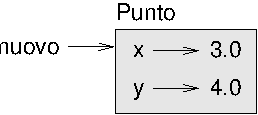
\includegraphics[scale=0.8]{figs/point.pdf}}
\caption{Diagramma di oggetto}
\label{fig.point}
\end{figure}


La variabile {\tt nuovo} fa riferimento ad un oggetto Punto che contiene due
   attributi, ed ogni attributo fa riferimento ad un numero in virgola mobile.

Potete leggere il valore di un attributo usando la stessa sintassi:

\begin{verbatim}
>>> nuovo.y
4.0
>>> x = nuovo.x
>>> x
3.0
\end{verbatim}
%
L'espressione {\tt nuovo.x} significa: ``Vai all'oggetto a cui {\tt nuovo}
fa riferimento e prendi il valore di {\tt x}''. In questo esempio, assegniamo il valore ad una variabile di nome {\tt x}. Non c'è conflitto tra la variabile locale {\tt x} e l'attributo {\tt x}.

Potete usare la notazione a punto all'interno di qualunque espressione, per esempio:

\begin{verbatim}
>>> print('(%g, %g)' % (nuovo.x, nuovo.y))
(3.0, 4.0)
>>> distanza = math.sqrt(nuovo.x**2 + nuovo.y**2)
>>> distanza
5.0
\end{verbatim}
%
Potete anche passare un'istanza come argomento, nel modo consueto:
\index{istanza!come argomento}

\begin{verbatim}
def stampa_punto(p):
    print('(%g, %g)' % (p.x, p.y))
\end{verbatim}
%
La funzione \verb"stampa_punto" riceve come argomento un Punto e lo visualizza in notazione matematica. Per invocarla, passate {\tt nuovo} come argomento:

\begin{verbatim}
>>> stampa_punto(nuovo)
(3.0, 4.0)
\end{verbatim}
%
Dentro alla funzione, il parametro {\tt p} è un alias di {\tt nuovo}, quindi se la funzione modifica {\tt p}, anche {\tt nuovo} viene modificato di conseguenza.
\index{alias}

Per esercizio, scrivete una funzione di nome \verb"distanza_tra_punti" che riceva due Punti come argomenti e ne restituisca la distanza.


\section{Rettangoli}
\label{rectangles}

A volte è abbastanza ovvio stabilire gli attributi necessari ad un oggetto, ma in altre occasioni occorre fare delle scelte. Immaginate di progettare una classe che rappresenti un rettangolo: quali attributi dovete usare per specificarne le dimensioni e la collocazione nel piano? Per semplicità, ignorate l'inclinazione e supponete che il rettangolo sia allineato in orizzontale o verticale.
\index{rappresentazione}

Ci sono almeno due possibili scelte: 

\begin{itemize}

\item Definire il centro del rettangolo oppure un angolo, e le sue dimensioni (altezza e larghezza);

\item Definire due angoli opposti.

\end{itemize}

È difficile stabilire quale delle due opzioni sia la migliore, ma giusto per fare un esempio implementeremo la prima.
\index{Rettangolo, classe}
\index{classe!Rettangolo}

Definiamo la nuova classe:

\begin{verbatim}
class Rettangolo:
    """Rappresenta un rettangolo. 

    attributi: larghezza, altezza, angolo.
    """
\end{verbatim}
%
La docstring elenca gli attributi:  {\tt larghezza} e
{\tt altezza} sono numeri; {\tt angolo} è un oggetto Punto che identifica l'angolo in basso a sinistra.

Per ottenere una rappresentazione di un rettangolo, dovete istanziare un oggetto Rettangolo e assegnare dei valori ai suoi attributi:

\begin{verbatim}
box = Rettangolo()
box.larghezza = 100.0
box.altezza = 200.0
box.angolo = Punto()
box.angolo.x = 0.0
box.angolo.y = 0.0
\end{verbatim}
%
L'espressione {\tt box.angolo.x} significa:
``Vai all'oggetto a cui {\tt box} fa riferimento e seleziona l'attributo chiamato
{\tt angolo}; poi vai a quell'oggetto e seleziona l'attributo chiamato {\tt x}.''

\begin{figure}
\centerline
{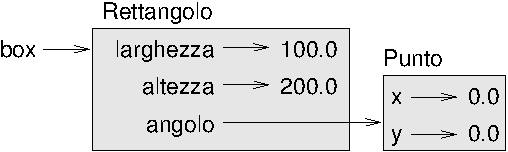
\includegraphics[scale=0.8]{figs/rectangle.pdf}}
\caption{Diagramma di oggetto.}
\label{fig.rectangle}
\end{figure}


La Figura~\ref{fig.rectangle} mostra lo stato di questo oggetto.
Un oggetto che è un attributo di un altro oggetto è detto {\bf oggetto contenuto} (embedded).
\index{diagramma!di stato}
\index{diagramma!di oggetto}
\index{oggetto contenuto (embedded)}


\section{Istanze come valori di ritorno}
\index{istanza!come valore di ritorno}
\index{valore di ritorno}

Le funzioni possono restituire istanze. Per esempio, \verb"trova_centro"
prende un oggetto {\tt Rettangolo} come argomento e restituisce un oggetto {\tt Punto} che contiene le coordinate del centro di {\tt Rettangolo}:

\begin{verbatim}
def trova_centro(rett):
    p = Punto()
    p.x = rett.angolo.x + rett.larghezza/2
    p.y = rett.angolo.y + rett.altezza/2
    return p
\end{verbatim}
%
Ecco un esempio che passa {\tt box} come argomento e assegna il Punto risultante a {\tt centro}:

\begin{verbatim}
>>> centro = trova_centro(box)
>>> stampa_punto(centro)
(50, 100)
\end{verbatim}
%

\section{Gli oggetti sono mutabili}
\index{oggetto!mutabile}
\index{mutabilità}

Potete cambiare lo stato di un oggetto con un'assegnazione ad uno dei suoi attributi. Per esempio, per cambiare le dimensioni di un rettangolo senza cambiarne la posizione, potete modificare i valori di {\tt larghezza} e {\tt altezza}:

\begin{verbatim}
box.larghezza = box.larghezza + 50
box.altezza = box.altezza + 100
\end{verbatim}
%
Potete anche scrivere delle funzioni che modificano oggetti. Per esempio,
\verb"accresci_rettangolo" prende un oggetto Rettangolo e due numeri,
{\tt dlargh} e {\tt dalt}, e li aggiunge alla larghezza e all'altezza del rettangolo:

\begin{verbatim}
def accresci_rettangolo(rett, dlargh, dalt):
    rett.larghezza += dlargh
    rett.altezza += dalt
\end{verbatim}
%
Ecco un esempio dell'effetto della funzione:

\begin{verbatim}
>>> box.larghezza, box.altezza
(150.0, 300.0)
>>> accresci_rettangolo(box, 50, 100)
>>> box.larghezza, box.altezza
(200.0, 400.0)
\end{verbatim}
%
Dentro la funzione, {\tt rett} è un alias di {\tt box}, pertanto quando la funzione modifica {\tt rett}, anche {\tt box} cambia.

Come esercizio, scrivete una funzione di nome \verb"sposta_rettangolo" che prenda come parametri un Rettangolo e due valori {\tt dx} e {\tt dy}.  La funzione deve spostare il rettangolo nel piano, aggiungendo {\tt dx} alla coordinata {\tt x} di {\tt angolo}, e aggiungendo {\tt dy} alla coordinata {\tt y} di {\tt angolo}.



\section{Copia}
\label{copying}
\index{alias}

Abbiamo già visto che gli alias possono rendere il programma difficile
   da leggere, perché una modifica in un punto del programma può dare degli effetti inattesi in un altro punto. Non è semplice tenere traccia di tutte le variabili che potrebbero fare riferimento ad un dato oggetto.
\index{copia!di un oggetto}
\index{oggetto!copia}
\index{copy, modulo}
\index{modulo!copy}

La copia di un oggetto è spesso una comoda alternativa all'alias.
Il modulo {\tt copy} contiene una funzione, anch'essa di nome {\tt copy}, che permette di duplicare qualsiasi oggetto:

\begin{verbatim}
>>> p1 = Punto()
>>> p1.x = 3.0
>>> p1.y = 4.0

>>> import copy
>>> p2 = copy.copy(p1)
\end{verbatim}
%
{\tt p1} e {\tt p2} contengono gli stessi dati, ma non sono lo stesso Punto.

\begin{verbatim}
>>> stampa_punto(p1)
(3, 4)
>>> stampa_punto(p2)
(3, 4)
>>> p1 is p2
False
>>> p1 == p2
False
\end{verbatim}
%
L'operatore {\tt is} indica che {\tt p1} e {\tt p2} non sono lo stesso oggetto, come volevasi dimostrare. Ma forse vi aspettavate che l'operatore {\tt ==} desse {\tt True}, perché i due punti contengono gli stessi dati. Invece, dovete sapere che, nel caso di istanze, il comportamento predefinito dell'operatore {\tt ==} è lo stesso dell'operatore {\tt is}: controlla l'identità dell'oggetto e non l'equivalenza. Questo perché, per i tipi personalizzati, Python non sa cosa debba essere considerato equivalente. O almeno, non lo sa ancora.
\index{is, operatore}
\index{operatore!is}
\index{identità}
\index{equivalenza}

Nell'usare {\tt copy.copy} per duplicare un Rettangolo, noterete che copia l'oggetto Rettangolo ma non l'oggetto Punto contenuto.
\index{oggetto contenuto (embedded)!copia}

\begin{verbatim}
>>> box2 = copy.copy(box)
>>> box2 is box
False
>>> box2.angolo is box.angolo
True
\end{verbatim}

\begin{figure}
\centerline
{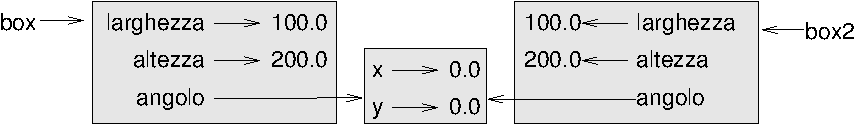
\includegraphics[scale=0.8]{figs/rectangle2.pdf}}
\caption{Diagramma di oggetto.}
\label{fig.rectangle2}
\end{figure}

La Figura~\ref{fig.rectangle2} mostra la situazione del diagramma di oggetto.
\index{diagramma!di stato}
\index{diagramma!di oggetto}

Questa operazione è chiamata {\bf copia shallow} (o copia superficiale) perché copia l'oggetto ed ogni riferimento che contiene, ma non gli oggetti contenuti.
\index{shallow, copia}
\index{copia!shallow}

Nella maggior parte dei casi, questo non è il comportamento ideale. Nel nostro esempio, invocare \verb"accresci_rettangolo" su uno dei Rettangoli non influenzerebbe l'altro, ma invocare \verb"sposta_rettangolo" su uno dei due, influenzerebbe entrambi! Tutto ciò genera confusione ed è foriero di errori.
\index{profonda, copia}
\index{copia!profonda}

Fortunatamente, il modulo {\tt copy} è dotato anche di un altro metodo chiamato {\tt deepcopy} che non solo copia l'oggetto, ma anche gli oggetti a cui si riferisce, e gli oggetti a cui questi ultimi a loro volta si riferiscono, e così via. Non vi sorprenderà che questa si chiami {\bf copia profonda}.
\index{deepcopy, funzione}
\index{funzione!deepcopy}

\begin{verbatim}
>>> box3 = copy.deepcopy(box)
>>> box3 is box
False
>>> box3.angolo is box.angolo
False
\end{verbatim}
%
{\tt box3} e {\tt box} sono oggetti completamente diversi.

Come esercizio, scrivete una versione di \verb"sposta_rettangolo" che crei e restituisca un nuovo Rettangolo anziché modificare quello di origine.



\section{Debug}
\label{hasattr}
\index{debug}

Iniziando a lavorare con gli oggetti, è facile imbattersi in alcuni nuovi tipi di eccezioni. Se cercate di accedere ad un attributo che non esiste, si verifica un {\tt AttributeError}:
\index{eccezione!AttributeError}
\index{AttributeError}

\begin{verbatim}
>>> p = Punto()
>>> p.x = 3
>>> p.y = 4
>>> p.z
AttributeError: Punto instance has no attribute 'z'
\end{verbatim}
%
Se non siete sicuri di che tipo sia un oggetto, potete chiederlo:
\index{type, funzione}
\index{funzione!type}

\begin{verbatim}
>>> type(p)
<class '__main__.Punto'>
\end{verbatim}
%
Si può usare anche {\tt isinstance} per controllare se un oggetto è un'istanza di una classe:
\index{isinstance, funzione}
\index{funzione!isinstance}

\begin{verbatim}
>>> isinstance(p, Punto)
True
\end{verbatim}
%
Se volete sapere se un oggetto ha un certo attributo, usate la funzione predefinita {\tt hasattr}:
\index{hasattr, funzione}
\index{funzione!hasattr}

\begin{verbatim}
>>> hasattr(p, 'x')
True
>>> hasattr(p, 'z')
False
\end{verbatim}
%
Il primo argomento può essere un qualunque oggetto, il secondo è una {\em
stringa} che contiene il nome dell'attributo.
\index{attributo}

Si può anche usare un'istruzione {\tt try} per controllare che l'oggetto contenga gli attributi che servono:
\index{try, istruzione}
\index{istruzione!try}

\begin{verbatim}
try:
    x = p.x
except AttributeError:
    x = 0
\end{verbatim}

Questa tecnica può facilitare la scrittura di funzioni che trattano tipi di dati differenti; vedremo altro su questo tema nel Paragrafo~\ref{polymorphism}.

\section{Glossario}

\begin{description}

\item[classe:] Tipo di dato personalizzato definito dal programmatore. Una definizione di classe crea un nuovo oggetto classe.
\index{classe}
\index{tipo!personalizzato}

\item[oggetto classe:] Oggetto che contiene le informazioni su un tipo personalizzato e che può essere usato per creare istanze del tipo.
\index{oggetto!classe}

\item[istanza:] Oggetto che appartiene ad una classe.
\index{istanza}

\item[istanziare:] Creare un nuovo oggetto.
\index{istanziare}

\item[attributo:] Uno dei valori associati ad un oggetto, dotato di un nome.
\index{attributo!istanza}
\index{istanza!attributo di}

\item[oggetto contenuto (embedded):] Oggetto che è contenuto come attributo di un altro oggetto (detto contenitore).
\index{oggetto contenuto (embedded)}

\item[copia shallow:] copia ``superficiale'' dei contenuti di un oggetto, senza includere alcun riferimento ad eventuali oggetti contenuti; è implementata grazie alla funzione {\tt copy} del modulo {\tt copy}.
\index{copia!shallow}

\item[copia profonda:] Copia del contenuto di un oggetto e anche degli eventuali
oggetti interni e degli oggetti a loro volta contenuti in essi; è implementata grazie alla funzione {\tt deepcopy} del modulo {\tt copy}.
\index{copia!profonda}

\item[diagramma di oggetto:] Diagramma che mostra gli oggetti, i loro attributi e i valori di questi ultimi.
\index{diagramma!di oggetto}

\end{description}


\section{Esercizi}

\begin{exercise}

Scrivete una definizione di classe di nome {\tt Cerchio}, avente gli attributi
{\tt centro} e {\tt raggio}, dove {\tt centro} è un oggetto Punto e {\tt raggio} è un numero.

Istanziate un oggetto Cerchio che rappresenti un cerchio con il centro nel punto $(150, 100)$ e di raggio 75.

Scrivete una funzione di nome \verb"punto_nel_cerchio", che prenda un Cerchio e un Punto e restituisca True se il punto giace dentro il cerchio, circonferenza compresa.

Scrivete una funzione di nome \verb"rett_nel_cerchio", che prenda un Cerchio e un  Rettangolo e restituisca True se il rettangolo giace interamente all'interno del cerchio, circonferenza compresa.

Scrivete una funzione di nome \verb"rett_cerchio_sovrapp", che prenda un Cerchio e un Rettangolo e restituisca True se almeno uno degli angoli del Rettangolo ricade all'interno del cerchio. Oppure, più difficile, se una qualunque porzione del Rettangolo ricade all'interno del cerchio.

Soluzione: \url{http://thinkpython2.com/code/Circle.py}.

\end{exercise}

\vspace{0.2in}
\begin{exercise}

Scrivete una funzione di nome \verb"disegna_rett" che prenda un oggetto Turtle e
un Rettangolo e usi la Tartaruga per disegnare il Rettangolo.  Vedere il
Capitolo~\ref{turtlechap} per esempi di uso degli oggetti Turtle.

Scrivete una funzione di nome \verb"disegna_cerchio" che prenda un oggetto Turtle e un Cerchio, e disegni il Cerchio.

Soluzione: \url{http://thinkpython2.com/code/draw.py}.

\end{exercise}



\chapter{Classi e funzioni}
\label{time}

Ora che sappiamo come creare dei nuovi tipi, il passo successivo è scrivere delle funzioni che prendano i tipi personalizzati come parametri e restituiscano dei risultati. In questo capitolo presenterò anche lo ``stile di programmazione funzionale'' e due nuove tecniche di sviluppo.

Il codice degli esempi di questo capitolo è scaricabile dal sito
\url{http://thinkpython2.com/code/Time1.py}.
Le soluzioni degli esercizi si trovano qui:
\url{http://thinkpython2.com/code/Time1_soln.py}.

\section{Tempo}
\label{isafter}

Facciamo un altro esempio di tipo personalizzato, creato dal programmatore, e definiamo una classe chiamata {\tt Tempo} che permette di rappresentare un'ora del giorno:
\index{tipo!personalizzato}
\index{Tempo, classe}
\index{classe!Tempo}

\begin{verbatim}
class Tempo:
    """Rappresenta un'ora del giorno.
       
    attributi: ora, minuto, secondo
    """
\end{verbatim}
%
Possiamo creare un nuovo oggetto {\tt Tempo}, assegnandogli tre attributi per le
ore, i minuti e i secondi:

\begin{verbatim}
tempo = Tempo()
tempo.ora = 11
tempo.minuto = 59
tempo.secondo = 30
\end{verbatim}
%
Il diagramma di stato dell'oggetto {\tt Tempo} è riportato in Figura~\ref{fig.time}.
\index{diagramma!di stato}
\index{diagramma!di oggetto}

Provate ora a scrivete una funzione di nome \verb"stampa_tempo" che accetti un oggetto Tempo come argomento e ne stampi il risultato nel formato {\tt ore:minuti:secondi}.
Suggerimento: la sequenza di formato \verb"'%.2d'" stampa un intero usando almeno due cifre, compreso uno zero iniziale dove necessario.

Scrivete poi una funzione booleana \verb"viene_dopo" che riceva come argomenti due oggetti Tempo, {\tt t1} e {\tt t2}, e restituisca {\tt True} se {\tt t1} è temporalmente successivo a {\tt t2} e {\tt False} in caso contrario.  Opzione più difficile: non usate un'istruzione {\tt if}.


\begin{figure}
\centerline
{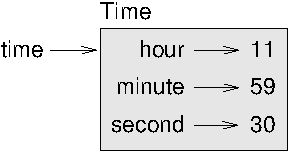
\includegraphics[scale=0.8]{figs/time.pdf}}
\caption{Diagramma di oggetto.}
\label{fig.time}
\end{figure}


\section{Funzioni pure}
\index{prototipo ed evoluzioni}
\index{tecnica di sviluppo!prototipo ed evoluzioni}

Nei prossimi paragrafi scriveremo due funzioni che sommano dei valori, espressi in termini temporali. Illustreremo così due tipi di funzioni: le funzioni pure e i modificatori. Dimostreremo anche una tecnica di sviluppo che chiameremo {\bf prototipo ed evoluzioni}, che è un modo di affrontare un problema complesso partendo da un prototipo semplice e trattando poi in maniera incrementale gli aspetti di maggior complessità.

Ecco un semplice prototipo della funzione \verb"somma_tempo":

\begin{verbatim}
def somma_tempo(t1, t2):
    somma = Tempo()
    somma.ora = t1.ora + t2.ora
    somma.minuto = t1.minuto + t2.minuto
    somma.secondo = t1.secondo + t2.secondo
    return somma
\end{verbatim}
%
La funzione crea un nuovo oggetto {\tt Tempo}, ne inizializza gli attributi, e restituisce un riferimento al nuovo oggetto. Questa è detta {\bf funzione pura},  perché non modifica alcuno degli oggetti che le vengono passati come argomento e, oltre a restituire un valore, non ha effetti visibili come visualizzare valori o chiedere input all'utente.
\index{funzione!pura}

Per provare questa funzione, creiamo due oggetti Tempo: {\tt inizio}
che contiene l'ora di inizio di un film, come {\em I Monty Python e il Sacro Graal}, e {\tt durata} che contiene la durata del film, che è un'ora e 35 minuti.
\index{Monty Python e il Sacro Graal}

\verb"somma_tempo" ci dirà a che ora finisce il film.

\begin{verbatim}
>>> inizio = Tempo()
>>> inizio.ora = 9
>>> inizio.minuto = 45
>>> inizio.secondo =  0

>>> durata = Tempo()
>>> durata.ora = 1
>>> durata.minuto = 35
>>> durata.secondo = 0

>>> fine = somma_tempo(inizio, durata)
>>> stampa_tempo(fine)
10:80:00
\end{verbatim}
%
Il risultato, {\tt 10:80:00} non è soddisfacente. Il problema è che questa funzione non gestisce correttamente i casi in cui la somma dei minuti e dei secondi equivale o supera sessanta. Quando questo accade, dobbiamo ``riportare'' i 60 secondi come minuto ulteriore, o i 60 minuti come ora ulteriore.
\index{addizione!con riporto}

Ecco allora una versione migliorata della funzione:

\begin{verbatim}
def somma_tempo(t1, t2):
    somma = Tempo()
    somma.ora = t1.ora + t2.ora
    somma.minuto = t1.minuto + t2.minuto
    somma.secondo = t1.secondo + t2.secondo

    if somma.secondo >= 60:
        somma.secondo -= 60
        somma.minuto += 1

    if somma.minuto >= 60:
        somma.minuto -= 60
        somma.ora += 1

    return somma
\end{verbatim}
%
Sebbene questa funzione sia corretta, comincia ad essere lunga. Tra poco vedremo un'alternativa più concisa.


\section{Modificatori}
\label{increment}
\index{modificatore}
\index{funzione!modificatore}

Ci sono casi in cui è utile che una funzione possa modificare gli oggetti che assume come parametri. I cambiamenti risulteranno visibili anche al chiamante. Funzioni che si comportano in questo modo sono dette {\bf modificatori}.
\index{incremento}

{\tt incremento}, che aggiunge un dato numero di secondi ad un oggetto {\tt Tempo}, può essere scritta intuitivamente come modificatore. Ecco un primo abbozzo della funzione:

\begin{verbatim}
def incremento(tempo, secondi):
    tempo.secondo += secondi

    if tempo.secondo >= 60:
        tempo.secondo -= 60
        tempo.minuto += 1

    if tempo.minuto >= 60:
        tempo.minuto -= 60
        tempo.ora += 1
\end{verbatim}
%
La prima riga esegue l'operazione di addizione fondamentale, mentre le successive controllano i casi particolari che abbiamo già visto prima.
\index{caso!particolare}

Questa funzione è corretta? Cosa succede se {\tt secondi}
è molto più grande di 60?  

In questo caso non è più sufficiente un unico riporto tra secondi e minuti: dobbiamo fare in modo di ripetere il controllo più volte, finché {\tt tempo.secondo} diventa minore di 60. Allora, una possibile soluzione è quella di sostituire le istruzioni {\tt if} con delle istruzioni {\tt while}.
Questo renderebbe la funzione corretta, ma non molto efficiente.

Come esercizio, scrivete una versione corretta di {\tt incremento} che non contenga alcun ciclo.

Tutto quello che può essere fatto con i modificatori può anche essere fatto con le funzioni pure. Tanto è vero che alcuni linguaggi di programmazione prevedono unicamente l'uso di funzioni pure. Si può affermare che i programmi che utilizzano funzioni pure sono più veloci da sviluppare e meno soggetti ad errori rispetto a quelli che fanno uso dei modificatori. Ma in qualche caso i modificatori convengono, perché i programmi funzionali risultano meno efficienti.

In linea generale, raccomando di usare funzioni pure quando possibile e usare i modificatori solo se c'è un evidente vantaggio nel farlo. Questo tipo di approccio può essere definito {\bf stile di programmazione funzionale}.
\index{stile di programmazione funzionale}

Per esercizio, scrivete una versione ``pura'' di {\tt incremento} che crei e restituisca un nuovo oggetto Tempo anziché modificare il parametro.


\section{Sviluppo prototipale e Sviluppo pianificato}
\label{prototype}
\index{prototipo ed evoluzioni}
\index{tecnica di sviluppo!prototipo ed evoluzioni}
\index{sviluppo pianificato}
\index{tecnica di sviluppo!pianificato}

La tecnica di sviluppo del programma che sto illustrando in questo Capitolo è detta ``prototipo ed evoluzioni'': per ogni funzione, si inizia scrivendo una versione grezza (prototipo) che effettui solo i calcoli fondamentali, provandola e via via migliorandola e correggendo gli errori.

Sebbene questo approccio possa essere abbastanza efficace, specie se non avete una adeguata conoscenza del problema, può condurre a scrivere del codice inutilmente complesso (perché deve affrontare molti casi particolari) e poco affidabile (dato che è difficile essere certi che tutti gli errori siano stati rimossi).

Un'alternativa è lo {\bf sviluppo pianificato}, nel quale una conoscenza approfondita degli aspetti del problema da affrontare rende la programmazione molto più semplice. Nel nostro caso, questa conoscenza sta nel fatto che l'oggetto Tempo è rappresentabile da un numero a tre cifre in base numerica 60! (vedere \url{http://it.wikipedia.org/wiki/Sistema_sessagesimale}.)  L'attributo
{\tt secondo} è la ``colonna delle unità'', l'attributo {\tt minuto}
è la ``colonna delle sessantine'', e l'attributo {\tt ora} quella della ``trecentosessantine''.
\index{sessagesimale}

Quando abbiamo scritto \verb"somma_tempo" e {\tt incremento}, stavamo a tutti gli effetti calcolando una addizione in base 60, e questo è il motivo per cui dovevamo gestire i riporti tra secondi e minuti e tra minuti e ore.
\index{addizione!con riporto}

Questa osservazione ci suggerisce un altro tipo di approccio al problema: possiamo convertire l'oggetto Tempo in un numero intero e approfittare della capacità del computer di effettuare operazioni sui numeri interi.

Questa funzione converte Tempo in un intero:

\begin{verbatim}
def tempo_in_int(tempo):
    minuti = tempo.ora * 60 + tempo.minuto
    secondi = minuti * 60 + tempo.secondo
    return secondi
\end{verbatim}
%
E questa è la funzione inversa, che converte un intero in un Tempo (ricordate che {\tt divmod} divide il primo argomento per il secondo e restituisce una tupla che contiene il quoziente e il resto).
\index{divmod}

\begin{verbatim}
def int_in_tempo(secondi):
    tempo = Tempo()
    minuti, tempo.secondo = divmod(secondi, 60)
    tempo.ora, tempo.minuto = divmod(minuti, 60)
    return tempo
\end{verbatim}
%
Per convincervi della esattezza di queste funzioni, pensateci un po' su e fate qualche prova. Una maniera di collaudarle è controllare che \verb"tempo_in_int(int_in_tempo(x)) == x" per vari valori di {\tt x}. Questo è un esempio di controllo di coerenza.
\index{coerenza, controllo di}

Quando vi siete convinti, potete usarle per riscrivere \verb"somma_tempo":

\begin{verbatim}
def somma_tempo(t1, t2):
    secondi = tempo_in_int(t1) + tempo_in_int(t2)
    return int_in_tempo(secondi)
\end{verbatim}
%
Questa versione è più concisa dell'originale e più facile da verificare.

Come esercizio, riscrivete {\tt incremento} usando \verb"tempo_in_int" e \verb"int_in_tempo".

Sicuramente, la conversione numerica da base 60 a base 10 e viceversa è più astratta e meno immediata rispetto al lavoro diretto con i tempi, che è istintivamente migliore.

Ma avendo l'intuizione di trattare i tempi come numeri in base 60, e    investendo il tempo necessario per scrivere le funzioni di conversione (\verb"tempo_in_int" e \verb"int_in_tempo"), abbiamo ottenuto un programma molto più corto, facile da leggere e correggere, e più affidabile.

Risulta anche più semplice aggiungere nuove caratteristiche, in un secondo tempo. Ad esempio, immaginate di dover sottrarre due Tempi per determinare l'intervallo trascorso. L'approccio iniziale avrebbe reso necessaria l'implementazione di una sottrazione con il prestito. Invece, con le funzioni di conversione, è molto più facile e rapido avere un programma corretto.
\index{sottrazione!con prestito}
\index{generalizzazione}

Paradossalmente, qualche volta rendere un problema più difficile (o più generale) lo rende più semplice, perché ci sono meno casi particolari da gestire e minori possibilità di errore.


\section{Debug}
\index{debug}

Un oggetto Tempo è ben impostato se i valori di {\tt minuto} e {\tt
secondo} sono compresi tra 0 e 60 (zero incluso ma 60 escluso) e se 
{\tt ora} è positiva.  {\tt ora} e {\tt minuto} devono essere interi, ma potremmo anche permettere a {\tt secondo} di avere una parte decimale.
\index{invariante}

Requisiti come questi sono detti {\bf invarianti} perché devono essere sempre soddisfatti. In altre parole, se non sono soddisfatti significa che qualcosa non è andato per il verso giusto.

Scrivere del codice per controllare le invarianti può servire a trovare errori e a identificarne le cause. Per esempio, potete scrivere una funzione
 \verb"tempo_valido" che prende un oggetto Tempo e restituisce
{\tt False} se viola un'invariante:

\begin{verbatim}
def tempo_valido(tempo):
    if tempo.ora < 0 or tempo.minuto < 0 or tempo.secondo < 0:
        return False
    if tempo.minuto >= 60 or tempo.secondo >= 60:
        return False
    return True
\end{verbatim}
%
All'inizio di ogni funzione, potete controllare l'argomento per assicurarvi della sua validità:
\index{raise, istruzione}
\index{istruzione!raise}

\begin{verbatim}
def somma_tempo(t1, t2):
    if not tempo_valido(t1) or not tempo_valido(t2):
        raise ValueError, 'oggetto Tempo non valido in somma_tempo'
    secondi = tempo_in_int(t1) + tempo_in_int(t2)
    return int_in_tempo(secondi)
\end{verbatim}
%
Oppure potete usare un'istruzione {\tt assert}, che controlla una data invariante e solleva un'eccezione in caso di difetti:
\index{assert, istruzione}
\index{istruzione!assert}

\begin{verbatim}
def somma_tempo(t1, t2):
    assert tempo_valido(t1) and tempo_valido(t2)
    secondi = tempo_in_int(t1) + tempo_in_int(t2)
    return int_in_tempo(secondi)
\end{verbatim}
%
Le istruzioni {\tt assert} sono utili perché permettono di distinguere il codice che tratta le condizioni normali da quello che controlla gli errori.


\section{Glossario}

\begin{description}

\item[prototipo ed evoluzioni:] Tecnica di sviluppo del programma a partire da un prototipo che viene gradualmente provato, esteso e migliorato.
\index{prototipo ed evoluzioni}

\item[sviluppo pianificato:] Tecnica di sviluppo che comporta profonde conoscenze del problema e maggiore pianificazione rispetto allo sviluppo incrementale o per prototipo.
\index{sviluppo pianificato}

\item[funzione pura:] Funzione che non modifica gli oggetti ricevuti come argomenti. La maggior parte delle funzioni pure sono produttive.
\index{funzione!pura}

\item[modificatore:] Funzione che cambia uno o più oggetti ricevuti come argomenti. La maggior parte dei modificatori sono vuoti, ovvero restituiscono {\tt None}.
\index{modificatore}

\item[stile di programmazione funzionale:] Stile di programmazione in cui la maggior parte delle funzioni è pura.
\index{stile di programmazione funzionale}

\item[invariante:] Condizione che deve sempre essere vera durante l'esecuzione del programma.
\index{invariante}

\item[istruzione assert:] Istruzione che controlla una condizione e solleva un'eccezione se fallisce.
\index{assert, istruzione}
\index{istruzione!assert}

\end{description}


\section{Esercizi}

Il codice degli esempi di questo capitolo è scaricabile dal sito
\url{http://thinkpython2.com/code/Time1.py}; le soluzioni degli esercizi si trovano in \url{http://thinkpython2.com/code/Time1_soln.py}.

\vspace{0.2in}
\begin{exercise}

Scrivete una funzione di nome \verb"moltiplica_tempo" che accetti un oggetto Tempo e un numero, e restituisca un nuovo oggetto Tempo che contiene il prodotto del Tempo iniziale per il numero.

Usate poi \verb"moltiplica_tempo" per scrivere una funzione che prenda un oggetto Tempo che rappresenta il tempo finale di una gara, e un numero che rappresenta la distanza percorsa, e restituisca un oggetto Tempo che rappresenta la media di gara (tempo al chilometro).
\index{cadenza di corsa}

\end{exercise}

\vspace{0.2in}
\begin{exercise}
\index{datetime, modulo}
\index{modulo!datetime}

Il modulo {\tt datetime} fornisce l'oggetto {\tt time}, simile all'oggetto Tempo di questo capitolo, ma che contiene un ricco insieme di metodi e operatori. Leggetene la documentazione sul sito \url{http://docs.python.org/3/library/datetime.html}.

\begin{enumerate}

\item Usate il modulo {\tt datetime} per scrivere un programma che ricavi la data odierna e visualizzi il giorno della settimana.

\item Scrivete un programma che riceva una data di nascita come input e visualizzi l'età dell'utente e il numero di giorni, ore, minuti e secondi che mancano al prossimo compleanno.
\index{compleanno}

\item Date due persone nate in giorni diversi, esiste un giorno in cui uno ha un'età doppia dell'altro. Questo è il loro ``Giorno del Doppio''. Scrivete un programma che prenda due date di nascita e calcoli quando si verifica il ``Giorno del Doppio''.

\item Un po' più difficile: scrivetene una versione più generale che calcoli il giorno in cui una persona ha $n$ volte l'età di un'altra.
\index{Giorno del Doppio}

\end{enumerate}

Soluzione: \url{http://thinkpython2.com/code/double.py}

\end{exercise}


\chapter{Classi e metodi}

Anche se abbiamo usato alcune delle caratteristiche {\em object-oriented} di Python, i programmi degli ultimi due capitoli non sono del tutto orientati agli oggetti, perché non mettono in evidenza le relazioni che esistono tra i tipi personalizzati e le funzioni che operano su di essi. Il passo successivo è di trasformare queste funzioni in metodi, in modo da rendere esplicite queste relazioni.

Il codice degli esempi di questo capitolo è scaricabile dal sito
\url{http://thinkpython2.com/code/Time2.py}, e le soluzioni degli esercizi da \url{http://thinkpython2.com/code/Point2_soln.py}.

\section{Funzionalità orientate agli oggetti}
\index{programmazione!orientata agli oggetti}

Python è un {\bf linguaggio di programmazione orientato agli oggetti}, in altre parole contiene delle funzionalità a supporto della programmazione orientata agli oggetti, che ha le seguenti caratteristiche distintive:

\begin{itemize}

\item I programmi includono definizioni di classi e metodi.  

\item Buona parte dell'elaborazione è espressa in termini di operazioni sugli oggetti.

\item Gli oggetti corrispondono spesso ad un oggetto o concetto del mondo reale, mentre i metodi che operano sugli oggetti corrispondono spesso al modo in cui gli oggetti interagiscono tra loro nella realtà quotidiana.

\end{itemize}

Per esempio, la classe {\tt Tempo} definita nel Capitolo~\ref{time}
corrisponde al modo in cui le persone pensano alle ore del giorno, e le funzioni che abbiamo definite corrispondono al tipo di operazioni che le persone fanno con il tempo. Allo stesso modo, le classi {\tt Punto} e {\tt Rettangolo} nel Capitolo~\ref{clobjects} corrispondono ai rispettivi concetti matematici.

Finora, non abbiamo tratto vantaggio dalle capacità di supporto della   programmazione orientata agli oggetti fornite da Python. A dire il vero, queste funzionalità non sono indispensabili; piuttosto, forniscono una sintassi alternativa per fare le cose che abbiamo già fatto. Ma in molti casi questa alternativa è più concisa e si adatta in modo più accurato alla struttura del programma.

Ad esempio, nel programma {\tt Time1.py} non c'è una chiara connessione tra la definizione della classe e le definizioni di funzione che seguono. A un esame più attento, è però evidente che tutte queste funzioni ricevono almeno un oggetto {\tt Tempo} come argomento.
\index{metodo}
\index{funzione}

Questa osservazione giustifica l'esistenza dei {\bf metodi}; un metodo è una funzione associata ad una particolare classe. Abbiamo già visto qualche metodo per le stringhe, le liste, i dizionari e le tuple. In questo capitolo, definiremo dei metodi per i tipi personalizzati.
\index{sintassi}
\index{semantica}
\index{tipo!personalizzato}

Da un punto di vista logico, i metodi sono la stessa cosa delle funzioni, ma con due differenze sintattiche:

\begin{itemize}

\item I metodi sono definiti all'interno di una definizione di classe, per      rendere esplicita la relazione tra la classe stessa ed il metodo.

\item La sintassi per invocare un metodo è diversa da quella usata per       chiamare una funzione.

\end{itemize}

Nei prossimi paragrafi prenderemo le funzioni scritte nei due capitoli    precedenti e le trasformeremo in metodi. Questa trasformazione è puramente meccanica e si fa seguendo una serie di passi: se siete in grado di convertire da funzione a metodo e viceversa, riuscirete anche a scegliere la forma migliore, qualsiasi cosa dobbiate fare.


\section{Stampa di oggetti}
\index{oggetto!stampa}

Nel Capitolo~\ref{time}, abbiamo definito una classe chiamata
{\tt Tempo}, e nel Paragrafo~\ref{isafter}, avete scritto una funzione di nome \verb"stampa_tempo":

\begin{verbatim}
class Tempo:
    """Rappresenta un'ora del giorno."""

def stampa_tempo(tempo):
    print('%.2d:%.2d:%.2d' % (tempo.ora, tempo.minuto, tempo.secondo))
\end{verbatim}
%
Per chiamare questa funzione occorre passare un oggetto {\tt Tempo} come    argomento:

\begin{verbatim}
>>> inizio = Tempo()
>>> inizio.ora = 9
>>> inizio.minuto = 45
>>> inizio.secondo = 00
>>> stampa_tempo(inizio)
09:45:00
\end{verbatim}
%
Per trasformare \verb"stampa_tempo" in un metodo, tutto quello che dobbiamo fare è spostare la definizione della funzione all'interno della definizione della classe. Notate bene la modifica nell'indentazione.
\index{indentazione}

\begin{verbatim}
class Tempo:
    def stampa_tempo(tempo):
        print('%.2d:%.2d:%.2d' % (tempo.ora, tempo.minuto, tempo.secondo))
\end{verbatim}
%
Ora ci sono due modi di chiamare \verb"stampa_tempo".  Il primo (e meno usato) è utilizzare la sintassi delle funzioni:
\index{funzione!sintassi}
\index{dot notation}


\begin{verbatim}
>>> Tempo.stampa_tempo(inizio)
09:45:00
\end{verbatim}
%
In questo uso della notazione a punto, {\tt Tempo} è il nome della classe e
 \verb"stampa_tempo" è il nome del metodo.  {\tt inizio} è passato come parametro.

Il secondo modo, più conciso, è usare la sintassi dei metodi:
\index{metodo!sintassi}

\begin{verbatim}
>>> inizio.stampa_tempo()
09:45:00
\end{verbatim}
%
Sempre usando la {\em dot notation}, \verb"stampa_tempo" è ancora il nome del metodo, mentre {\tt inizio} è l'oggetto sul quale il metodo è invocato, che è chiamato il {\bf soggetto}.  Come il soggetto di una frase è ciò a cui si riferisce la frase, il soggetto del metodo è ciò a cui si applica l'invocazione del metodo.
\index{soggetto}

All'interno del metodo, il soggetto viene assegnato al primo dei parametri: in questo caso, {\tt inizio} viene assegnato a {\tt tempo}.
\index{self (nome di parametro)}
\index{parametro!self}

Per convenzione, il primo parametro di un metodo viene chiamato {\tt self}, di conseguenza è bene riscrivere \verb"stampa_tempo" così:

\begin{verbatim}
class Tempo:
    def stampa_tempo(self):
        print('%.2d:%.2d:%.2d' % (self.ora, self.minuto, self.secondo))
\end{verbatim}
%
La ragione di questa convenzione è una metafora implicita:
\index{metafora, invocazione di metodo}

\begin{itemize}

\item La sintassi di una chiamata di funzione, \verb"stampa_tempo(inizio)",
  suggerisce che la funzione è la parte attiva, che dice qualcosa del tipo: ``Ehi, \verb"stampa_tempo"!  Ti passo un oggetto da stampare!''

\item Nella programmazione orientata agli oggetti, la parte attiva sono gli oggetti.  L'invocazione di un metodo come \verb"inizio.stampa_tempo()" dice:
  ``Ehi, {\tt inizio}!  Stampa te stesso!''

\end{itemize}

Questo cambio di prospettiva sarà anche più elegante, ma cogliere la sua utilità non è immediato. Nei semplici esempi che abbiamo visto finora, può non esserlo. Ma in altri casi, spostare la responsabilità dalle funzioni agli oggetti rende possibile scrivere funzioni (o metodi) più versatili e rende più facile mantenere e riusare il codice.

Come esercizio, riscrivete \verb"tempo_in_int" (vedere Paragrafo~\ref{prototype}) come metodo.
Potreste pensare di riscrivere anche \verb"int_in_tempo" come metodo, ma non avrebbe molto senso: non vi sarebbe alcun oggetto sul quale invocarlo.



\section{Un altro esempio}
\index{incremento}

Ecco una versione di {\tt incremento} (vedere Paragrafo~\ref{increment}),
riscritto come metodo:

\begin{verbatim}
# all'interno della classe Tempo:

    def incremento(self, secondi):
        secondi += self.tempo_in_int()
        return int_in_tempo(secondi)
\end{verbatim}
%
Questa versione presuppone che \verb"tempo_in_int" sia stato scritto come metodo.  Notate anche che si tratta di una funzione pura e non un modificatore.

Ecco come invocare {\tt incremento}:

\begin{verbatim}
>>> inizio.stampa_tempo()
09:45:00
>>> fine = inizio.incremento(1337)
>>> fine.stampa_tempo()
10:07:17
\end{verbatim}
%
Il soggetto, {\tt inizio}, viene assegnato quale primo parametro, a
{\tt self}.  L'argomento, {\tt 1337}, viene assegnato quale secondo parametro, a {\tt secondi}.

Questo meccanismo può confondere le idee, specie se commettete qualche errore. Per esempio, se invocate {\tt incremento} con due argomenti ottenete:
\index{eccezione!TypeError}
\index{TypeError}

\begin{verbatim}
>>> fine = inizio.incremento(1337, 460)
TypeError: incremento() takes 2 positional arguments but 3 were given
\end{verbatim}
%
Il messaggio di errore a prima vista non è chiaro, perché ci sono solo due argomenti tra parentesi. Ma bisogna tener conto che anche il soggetto è considerato un argomento, ecco perché in totale fanno tre.

Tra parentesi, un {\bf argomento posizionale} è un argomento privo di nome di un parametro; cioè, non è un argomento con nome. In questa chiamata di funzione:
\index{posizionale, argomento}
\index{argomento!posizionale}

\begin{verbatim}
sketch(pappagallo, gabbia, morto=True)
\end{verbatim}

{\tt pappagallo} e {\tt gabbia} sono argomenti posizionali, e {\tt morto} è un argomento con nome.


\section{Un esempio più complesso}

\verb"viene_dopo" (vedere Paragrafo~\ref{isafter}) è leggermente più complesso da riscrivere come metodo, perché richiede come parametri due oggetti Tempo. In questo caso, la convenzione prevede di denominare il primo parametro {\tt self} e il secondo {\tt other}:
\index{other (nome di parametro)}
\index{parametro!other}

\begin{verbatim}
# all'interno della classe Tempo:

    def viene_dopo(self, other):
        return self.tempo_in_int() > other.tempo_in_int()
\end{verbatim}
%
Per usare questo metodo, lo dovete invocare su un oggetto e passare l'altro come argomento:

\begin{verbatim}
>>> fine.viene_dopo(inizio)
True
\end{verbatim}
%
Una particolarità di questa sintassi è che si legge quasi come in italiano:
``fine viene dopo inizio?''


\section{Il metodo speciale init}
\index{init, metodo}
\index{metodo!init}

Il metodo init (abbreviazione di {\em initialization}, ovvero inizializzazione) è un metodo speciale che viene invocato quando un oggetto viene istanziato. Il suo nome completo è \verb"__init__" (due caratteri underscore, 
seguiti da {\tt init}, e da altri due  underscore). Un metodo init per la classe  {\tt Tempo} può essere il seguente:

\begin{verbatim}
# all'interno della classe Tempo:

    def __init__(self, ora=0, minuto=0, secondo=0):
        self.ora = ora
        self.minuto = minuto
        self.secondo = secondo
\end{verbatim}
%
È prassi che i parametri di \verb"__init__" abbiano gli stessi nomi degli attributi. L'istruzione

\begin{verbatim}
        self.ora = ora
\end{verbatim}
%
memorizza il valore del parametro {\tt ora} come attributo di {\tt self}.
\index{parametro!opzionale}
\index{valore di default}
\index{sovrascrittura}

I parametri sono opzionali, quindi se chiamate {\tt Tempo} senza argomenti, ottenete i valori di default.

\begin{verbatim}
>>> tempo = Tempo()
>>> tempo.stampa_tempo()
00:00:00
\end{verbatim}
%
Se fornite un argomento, esso va a sovrascrivere {\tt ora}:

\begin{verbatim}
>>> tempo = Tempo (9)
>>> tempo.stampa_tempo()
09:00:00
\end{verbatim}
%
Se ne fornite due, sovrascrivono {\tt ora} e {\tt minuto}.

\begin{verbatim}
>>> tempo = Tempo(9, 45)
>>> tempo.stampa_tempo()
09:45:00
\end{verbatim}
%
E se ne fornite tre, sovrascrivono tutti e tre i valori di default.

Per esercizio, scrivete un metodo init per la classe {\tt Punto} che prenda {\tt x} e {\tt y} come parametri opzionali e li assegni agli attributi corrispondenti.
\index{Punto, classe}
\index{classe!Punto}

\section{Il metodo speciale {\tt \_\_str\_\_}}
\index{str metodo@\_\_str\_\_, metodo}
\index{metodo!\_\_str\_\_}

\verb"__str__" è un altro metodo speciale, come \verb"__init__",
che ha lo scopo di restituire una rappresentazione di un oggetto in forma di stringa.
\index{rappresentazione!di stringa}

Ecco ad esempio un metodo {\tt str} per un oggetto Tempo:

\begin{verbatim}
# all'interno della classe Tempo:

    def __str__(self):
        return '%.2d:%.2d:%.2d' % (self.ora, self.minuto, self.secondo)
\end{verbatim}
%
Quando stampate un oggetto con l'istruzione di stampa, Python invoca il metodo {\tt str}:
\index{stampa, istruzione di}
\index{istruzione!di stampa}

\begin{verbatim}
>>> tempo = Tempo(9, 45)
>>> print(tempo)
09:45:00
\end{verbatim}
%
Personalmente, quando scrivo una nuova classe, quasi sempre inizio con lo scrivere \verb"__init__", che rende più facile istanziare un oggetto, e 
\verb"__str__", che è utile per il debugging.

Come esercizio, scrivete un metodo {\tt str} per la classe {\tt Punto}.  Create un oggetto Punto e stampatelo.


\section{Operator overloading}
\label{operator.overloading}

Nei tipi personalizzati, avete la possibilità di adattare il comportamento degli operatori attraverso la definizione di altri appositi metodi speciali. Per esempio se definite il metodo speciale di nome \verb"__add__" per la classe {\tt Tempo}, potete poi usare l'operatore {\tt +} sugli oggetti Tempo.
\index{tipo!personalizzato}

Ecco come potrebbe essere scritta la definizione:
\index{add, metodo}
\index{metodo!add}

\begin{verbatim}
# all'interno della classe Tempo:

    def __add__(self, other):
        secondi = self.tempo_in_int() + other.tempo_in_int()
        return int_in_tempo(secondi)
\end{verbatim}
%
Ed ecco come può essere usata:

\begin{verbatim}
>>> inizio = Tempo(9, 45)
>>> durata = Tempo(1, 35)
>>> print(inizio + durata)
11:20:00
\end{verbatim}
%
Quando applicate l'operatore {\tt +} agli oggetti Tempo, Python invoca
\verb"__add__".  Quando stampate il risultato, Python invoca 
\verb"__str__".  Accadono parecchie cose, dietro le quinte!
\index{operator overloading}

Cambiare il comportamento degli operatori in modo che funzionino con i tipi personalizzati è chiamato {\bf operator overloading} (letteralmente, sovraccarico degli operatori). In Python, per ogni operatore esiste un corrispondente metodo speciale, come
\verb"__add__".  Per ulteriori dettagli consultate
\url{http://docs.python.org/2/reference/datamodel.html#specialnames}.

Esercitatevi scrivendo un metodo {\tt add} per la classe Punto.  


\section{Smistamento in base al tipo}

Nel Paragrafo precedente abbiamo sommato due oggetti Tempo, ma potrebbe anche capitare di voler aggiungere un numero intero a un oggetto Tempo. Quella che segue è una versione di \verb"__add__"
che controlla il tipo di {\tt other} e, a seconda dei casi, invoca o
\verb"somma_tempo" o {\tt incremento}:

\begin{verbatim}
# all'interno della classe Tempo:

    def __add__(self, other):
        if isinstance(other, Tempo):
            return self.somma_tempo(other)
        else:
            return self.incremento(other)

    def somma_tempo(self, other):
        secondi = self.tempo_in_int() + other.tempo_in_int()
        return int_in_tempo(secondi)

    def incremento(self, secondi):
        secondi += self.tempo_in_int()
        return int_in_tempo(secondi)
\end{verbatim}
%
La funzione predefinita {\tt isinstance} prende un valore e un oggetto classe, e restiutisce {\tt True} se il valore è un'istanza della classe.
\index{isinstance, funzione}
\index{funzione!isinstance}

Quindi, se {\tt other} è un oggetto Tempo, \verb"__add__" invoca
\verb"somma_tempo".  Altrimenti, considera che il parametro sia un numero, e invoca {\tt incremento}.  Questa operazione è detta {\bf smistamento in base al tipo}, perché invia il calcolo a metodi diversi a seconda del tipo di argomento.
\index{smistamento in base al tipo}

Ecco degli esempi che usano l'operatore {\tt +} con tipi diversi:

\begin{verbatim}
>>> inizio = Tempo(9, 45)
>>> durata = Tempo(1, 35)
>>> print(inizio + durata)
11:20:00
>>> print(inizio + 1337)
10:07:17
\end{verbatim}
%
Sfortunatamente, questa implementazione di addizione non è commutativa. Se l'intero è il primo operando vi risulterà infatti:
\index{commutatività}

\begin{verbatim}
>>> print(1337 + inizio)
TypeError: unsupported operand type(s) for +: 'int' and 'instance'
\end{verbatim}
%
Il problema è che, invece di chiedere all'oggetto Tempo di aggiungere un intero, Python chiede all'intero di aggiungere un oggetto Tempo, ma l'intero non ha la minima idea di come farlo. Ma a questo c'è una soluzione intelligente: il metodo speciale \verb"__radd__", che sta per {\em right-side add} (``addizione lato destro'').
Questo metodo viene invocato quando un oggetto Tempo compare sul lato destro dell'operatore {\tt +}.  Eccone la definizione:
\index{radd, metodo}
\index{metodo!radd}

\begin{verbatim}
# all'interno della classe Tempo:

    def __radd__(self, other):
        return self.__add__(other)
\end{verbatim}
%
Ed eccolo in azione:

\begin{verbatim}
>>> print(1337 + inizio)
10:07:17
\end{verbatim}
%

Come esercizio, scrivete un metodo {\tt add} per i Punti che possa funzionare sia con un oggetto Punto che con una tupla:  

\begin{itemize}

\item Se il secondo operando è un Punto, il metodo deve restituire un nuovo Punto la cui coordinata $x$ sia la somma delle coordinate $x$ degli operandi, e lo stesso per le coordinate $y$.

\item Se il secondo operando è una tupla, il metodo deve aggiungere il primo elemento della tupla alla coordinata $x$ e il secondo elemento alla coordinata $y$, e restituire un nuovo Punto con le coordinate risultanti.

\end{itemize}



\section{Polimorfismo}
\label{polymorphism}

Lo smistamento in base al tipo è utile all'occorrenza, ma (fortunatamente) non è sempre necessario. Spesso potete evitarlo scrivendo le funzioni in modo che operino correttamente con argomenti di tipo diverso.
\index{smistamento in base al tipo}

Molte delle funzioni che abbiamo scritto per le stringhe, funzioneranno anche con qualsiasi altro tipo di sequenza.
Per esempio, nel Paragrafo~\ref{histogram}
abbiamo usato {\tt istogramma} per contare quante volte ciascuna lettera appare in una parola.

\begin{verbatim}
def istogramma(s):
    d = dict()
    for c in s:
        if c not in d:
            d[c] = 1
        else:
            d[c] = d[c]+1
    return d
\end{verbatim}
%
Questa funzione è applicabile anche a liste, tuple e perfino dizionari, a condizione che gli elementi di {\tt s} siano idonei all'hashing, in modo da poter essere usati come chiavi in {\tt d}.

\begin{verbatim}
>>> t = ['spam', 'uovo', 'spam', 'spam', 'bacon', 'spam']
>>> istogramma(t)
{'bacon': 1, 'uovo': 1, 'spam': 4}
\end{verbatim}
%
Le funzioni che sono in grado di operare con tipi diversi sono dette {\bf polimorfiche}.
Il polimorfismo facilita il riuso del codice.  Ad esempio, la funzione predefinita {\tt sum}, che addiziona gli elementi di una sequenza, funziona alla sola condizione che gli elementi della sequenza siano addizionabili.
\index{polimorfismo}

Dato che agli oggetti Tempo abbiamo fornito un metodo {\tt add}, funzionano con
{\tt sum}:

\begin{verbatim}
>>> t1 = Tempo(7, 43)
>>> t2 = Tempo(7, 41)
>>> t3 = Tempo(7, 37)
>>> totale = sum([t1, t2, t3])
>>> print(totale)
23:01:00
\end{verbatim}
%
In linea generale, se tutte le operazioni all'interno di una funzione si possono applicare ad un dato tipo, la funzione può operare con quel tipo.

Il miglior genere di polimorfismo è quello involontario, quando scoprite che una funzione che avete già scritto può essere applicata anche ad un tipo che non avevate previsto.


\section{Debug}
\index{debug}

È consentito aggiungere attributi in qualsiasi momento dell'esecuzione di un programma, ma se avete oggetti dello stesso tipo che non hanno gli stessi attributi, è facile generare errori. Inizializzare tutti gli attributi di un oggetto nel metodo init è considerata una prassi migliore.
\index{init, metodo}
\index{attributo!inizializzazione}

Se non siete certi che un oggetto abbia un particolare attributo, potete usare la funzione predefinita {\tt hasattr} (vedere Paragrafo~\ref{hasattr}).
\index{hasattr, funzione}
\index{funzione!hasattr}
\index{dict, attributo@\_\_dict\_\_ attributo}
\index{attributo!\_\_dict\_\_}

Un altro modo di accedere agli attributi è la funzione predefinita {\tt vars}, che prende un oggetto e restituisce un dizionario che fa corrispondere nomi degli attributi (come stringhe) e i relativi valori:

\begin{verbatim}
>>> p = Punto(3, 4)
>>> vars(p)
{'y': 4, 'x': 3}
\end{verbatim}
%
Per gli scopi del debug, può essere utile tenere questa funzione a portata di mano:

\begin{verbatim}
def stampa_attributi(oggetto):
    for attr in vars(oggetto):
        print(attr, getattr(oggetto, attr))
\end{verbatim}
%
\verb"stampa_attributi" attraversa il dizionario e stampa ciascun nome di attributo con il suo valore.
\index{attraversamento!dizionario}
\index{dizionario!attraversamento}

La funzione predefinita {\tt getattr} prende un oggetto e un nome di attributo (come stringa) e restituisce il valore dell'attributo.
\index{getattr, funzione}
\index{funzione!getattr}


\section{Interfaccia e implementazione}

Uno degli scopi della progettazione orientata agli oggetti è di rendere più agevole la manutenzione del software, che significa poter mantenere il programma funzionante quando altre parti del sistema vengono cambiate e poter modificare il programma per adeguarlo a dei nuovi requisiti.
\index{interfaccia}
\index{implementazione}
\index{manutenzione}
\index{progettazione!orientata agli oggetti}

Un principio di progettazione che aiuta a raggiungere questo obiettivo è di tenere le interfacce separate dalle implementazioni.
Per gli oggetti, significa che i metodi esposti da una classe non devono dipendere da come vengono rappresentati gli attributi.
\index{attributo}

Per esempio, in questo capitolo abbiamo sviluppato una classe che rappresenta un'ora del giorno. I metodi esposti da questa classe comprendono
\verb"tempo_in_int", \verb"viene_dopo", e \verb"somma_tempo".

Quei metodi possono essere implementati in diversi modi. I dettagli dell'implementazione dipendono da come rappresentiamo il tempo. In questo capitolo, gli attributi di un oggetto {\tt Tempo} sono {\tt ora}, {\tt minuto}, e {\tt secondo}.

Come alternativa, avremmo potuto sostituire quegli attributi con un singolo numero intero, come secondi trascorsi dalla mezzanotte. Con questa implementazione, alcuni metodi come \verb"viene_dopo", sarebbero diventati più facili da scrivere, ma altri più difficili.

Dopo aver sviluppato una nuova classe, potreste scoprire una implementazione migliore. Se altre parti del programma usano quella classe, cambiare l'interfaccia può essere dispendioso in termini di tempo e fonte di errori.  

Ma se avete progettato l'interfaccia accuratamente, potete cambiare l'implementazione senza cambiare l'interfaccia, che significa che non occorre cambiare altre parti del programma.


\section{Glossario}

\begin{description}

\item[linguaggio orientato agli oggetti:] Linguaggio che possiede delle caratteristiche, come tipi personalizzati e metodi, che facilitano la programmazione orientata agli oggetti. 
\index{linguaggio!orientato agli oggetti}

\item[programmazione orientata agli oggetti:] Paradigma di programmazione in cui i dati e le operazioni sui dati vengono organizzati in classi e metodi.
\index{programmazione!orientata agli oggetti}

\item[metodo:] Funzione definita all'interno di una definizione di classe e che viene invocata su istanze di quella classe.
\index{metodo}

\item[soggetto:] L'oggetto sul quale viene invocato un metodo.
\index{soggetto}

\item[argomento posizionale:] Un argomento che non include il nome di un
parametro, ovvero non è un argomento con nome.
\index{posizionale, argomento}
\index{argomento!posizionale}

\item[operator overloading:] Cambiare il comportamento di un operatore come
{\tt +} in modo che funzioni con un tipo personalizzato.
\index{overloading}
\index{operator overloading}

\item[smistamento in base al tipo:] Schema di programmazione che controlla il tipo di un operando e invoca funzioni diverse in base ai diversi tipi.
\index{smistamento in base al tipo}

\item[polimorfico:] Di una funzione che può operare con più di un tipo di dati.
\index{polimorfismo}

\item[information hiding:] Principio per cui l'interfaccia di un oggetto non deve dipendere dalla sua implementazione, con particolare riferimento alla rappresentazione dei suoi attributi.
\index{information hiding}


\end{description}

\section{Esercizi}

\vspace{0.2in}
\begin{exercise}

Scaricate il codice degli esempi di questo capitolo
(\url{http://thinkpython2.com/code/Time2.py}).  Cambiate gli attributi di {\tt Tempo} con un singolo intero che rappresenta i secondi dalla mezzanotte. Quindi modificate i metodi (e la funzione \verb"int_in_tempo") in modo che funzionino con la nuova implementazione. Non dovete cambiare il codice di prova in {\tt main}.  Quando avete finito, l'output dovrebbe essere lo stesso di prima. Soluzione: \url{http://thinkpython2.com/code/Time2_soln.py}.
\end{exercise}

\vspace{0.2in}
\begin{exercise}
\label{kangaroo}
\index{valore di default!evitare i mutabili}
\index{oggetto mutabile, come valore di default}
\index{peggior bug}
\index{bug!il peggiore}
\index{Canguro, classe}
\index{classe!Canguro}

Questo esercizio è un aneddoto monitorio su uno degli errori più comuni e difficili da trovare in Python. Scrivete una definizione di una classe di nome {\tt Canguro} con i metodi seguenti:

\begin{enumerate}

\item Un metodo \verb"__init__" che inizializza un attributo di nome
\verb"contenuto_tasca" ad una lista vuota.

\item Un metodo di nome \verb"intasca" che prende un oggetto di qualsiasi tipo e lo inserisce in \verb"contenuto_tasca".

\item Un metodo \verb"__str__" che restituisce una stringa di rappresentazione  dell'oggetto Canguro e dei contenuti della tasca.

\end{enumerate}
%
Provate il codice creando due oggetti {\tt Canguro}, assegnandoli a variabili di nome {\tt can} e {\tt guro}, e aggiungendo poi {\tt guro} al contenuto della tasca di {\tt can}.

Scaricate \url{http://thinkpython2.com/code/BadKangaroo.py}.  Contiene una soluzione al problema precedente, ma con un grande e serio errore. Trovatelo e sistematelo.  

Se vi bloccate, potete scaricare
\url{http://thinkpython2.com/code/GoodKangaroo.py}, che spiega il problema e illustra una soluzione.
\index{alias}
\index{contenuto, oggetto}
\index{oggetto!contenuto}

\end{exercise}


\chapter{Ereditarietà}

La caratteristica più frequentemente associata alla programmazione orientata agli oggetti è l'{\bf ereditarietà}, che è la capacità di definire una nuova classe come versione modificata di una classe già esistente.
In questo capitolo illustrerò l'ereditarietà usando delle classi che rappresentano carte da gioco, mazzi di carte e mani di poker. 

Se non giocate a poker, potete leggere qualcosa in proposito sul sito \url{http://it.wikipedia.org/wiki/Poker}, ma non è un obbligo: vi spiegherò quello che serve.
\index{carte da gioco}
\index{poker}
\index{mazzo}

Il codice degli esempi di questo capitolo è scaricabile da
\url{http://thinkpython2.com/code/Card.py}.


\section{Oggetti Carta}

In un mazzo ci sono 52 carte, e ciascuna appartiene a uno tra quattro semi e a uno tra tredici valori. I semi sono Picche, Cuori, Quadri e Fiori (in ordine decrescente nel gioco del bridge). I valori sono Asso, 2, 3, 4, 5, 6, 7, 8, 9, 10, Fante, Regina e Re. A seconda del gioco, l'Asso può essere superiore al Re o inferiore al 2.
\index{valore (delle carte da gioco)}
\index{seme}

Se vogliamo definire un nuovo oggetto che rappresenti una carta da gioco, è evidente quali attributi dovrebbe avere: {\tt valore} e
{\tt seme}.  È meno evidente stabilire di che tipo devono essere questi attributi. Una possibilità è usare stringhe contenenti parole come
\verb"'Picche'" per i semi e \verb"'Regina'" per i valori. Ma un problema di questa implementazione è che non è facile confrontare le carte per vedere quale abbia un seme o un valore superiore.
\index{codificare}
\index{criptare}
\index{corrispondenza}
\index{rappresentazione}

Un'alternativa è usare degli interi per {\bf codificare} valori e semi.
In questo contesto, ``codificare'' significa determinare una corrispondenza tra numeri e semi o numeri e valori. Non significa che debba essere un segreto (quello è ``criptare'').

\newcommand{\mymapsto}{$\mapsto$}

Per esempio, questa tabella mostra i semi e i corrispondenti codici interi:

\begin{tabular}{l c l}
Picche & \mymapsto & 3 \\
Cuori & \mymapsto & 2 \\
Quadri & \mymapsto & 1 \\
Fiori & \mymapsto & 0
\end{tabular}

In questo modo, diventa facile confrontare le carte: siccome ai semi più alti corrispondono numeri più alti, si possono confrontare i semi confrontando i loro codici corrispondenti.

Nel caso dei valori, la corrispondenza è abbastanza immediata: ogni valore numerico corrisponde al rispettivo intero, mentre per le figure:

\begin{tabular}{l c l}
Fante & \mymapsto & 11 \\
Regina & \mymapsto & 12 \\
Re & \mymapsto & 13 \\
\end{tabular}

Uso il simbolo \mymapsto~per chiarire che queste corrispondenze non fanno parte del programma Python. Fanno parte del progetto del programma, ma non compaiono esplicitamente nel codice.
\index{Carta, classe}
\index{classe!Carta}

Ecco come si può presentare la definizione di classe per {\tt Carta}:

\begin{verbatim}
class Carta:
    """Rappresenta una carta da gioco standard."""

    def __init__(self, seme=0, valore=2):
        self.seme = seme
        self.valore = valore
\end{verbatim}
%
Come al solito, il metodo init prevede un parametro opzionale per ciascun attributo. La carta di default è il 2 di fiori.
\index{init, metodo}
\index{metodo!init}

Per creare una carta, si chiama la classe {\tt Carta} con il seme e il valore desiderati.

\begin{verbatim}
regina_di_quadri = Carta(1, 12)
\end{verbatim}
%


\section{Attributi di classe}
\label{class.attribute}
\index{classe!attributo di}
\index{attributo!di classe}

Per stampare gli oggetti Carta in un modo comprensibile agli utenti, occorre stabilire una corrispondenza dai codici interi ai relativi semi e valori. Un modo naturale per farlo è usare delle liste di stringhe, che assegneremo a degli {\bf attributi di classe}:

\begin{verbatim}
# all'interno della classe Carta:

    nomi_semi = ['Fiori', 'Quadri', 'Cuori', 'Picche']
    nomi_valori = [None, 'Asso', '2', '3', '4', '5', '6', '7', 
              '8', '9', '10', 'Fante', 'Regina', 'Re']

    def __str__(self):
        return '%s di %s' % (Carta.nomi_valori[self.valore],
                             Carta.nomi_semi[self.seme])
\end{verbatim}
%
Variabili come \verb"nomi_semi" e \verb"nomi_valori", che sono definite dentro la classe ma esternamente a ogni metodo, sono chiamate attributi di classe perché sono associati all'oggetto classe {\tt Carta}.
\index{istanza!attributo di}
\index{attributo!di istanza}

Questo termine li distingue da variabili come {\tt seme} e {\tt
  valore}, che sono chiamati {\bf attributi di istanza} perché sono associati ad una specifica istanza.
\index{dot notation}

Ad entrambi i tipi si accede usando la notazione a punto. Per esempio in \verb"__str__", {\tt self} è un oggetto carta e {\tt self.valore} è il suo valore.  Allo stesso modo, {\tt Carta} è un oggetto classe, e \verb"Carta.nomi_valori" è una lista di stringhe associata alla classe.

Ogni carta ha i suoi propri {\tt seme} e {\tt valore}, ma esiste una sola copia di \verb"nomi_semi" e \verb"nomi_valori".

Mettendo insieme il tutto, l'espressione
\verb"Carta.nomi_valori[self.valore]" significa ``usa l'attributo {\tt valore} dell'oggetto {\tt self} come indice nella lista \verb"nomi_valori"
dalla classe {\tt Carta}, e seleziona la stringa corrispondente.''

Il primo elemento della lista \verb"nomi_valori" è {\tt None} perché non esiste una carta di valore zero. Includendo {\tt None} come segnaposto, otteniamo una corrispondenza corretta per cui all'indice 2 corrisponde la stringa \verb"'2'", e così via. Per evitare questo trucco, avremmo potuto usare un dizionario al posto di una lista.

Con i metodi che abbiamo visto fin qui, possiamo creare e stampare i nomi delle carte:

\begin{verbatim}
>>> carta1 = Carta(2, 11)
>>> print(carta1)
Fante di Cuori
\end{verbatim}

\begin{figure}
\centerline
{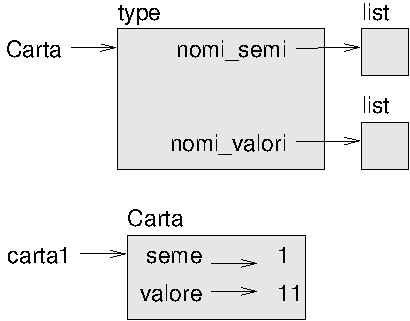
\includegraphics[scale=0.8]{figs/card1.pdf}}
\caption{Diagramma di oggetto.}
\label{fig.card1}
\end{figure}

La Figura~\ref{fig.card1} è un diagramma dell'oggetto classe {\tt Carta} e di una Carta, sua istanza.
{\tt Carta} è un oggetto classe, quindi è di tipo {\tt type}.  {\tt
carta1} invece è di tipo {\tt Carta}.  (Per motivi di spazio ho omesso i contenuti di \verb"nomi_semi" e \verb"nomi_valori").
\index{diagramma!di stato}
\index{diagramma!di oggetto}

\section{Confrontare le carte}
\label{comparecard}
\index{operatore!relazionale}


Per i tipi predefiniti, esistono gli operatori relazionali
({\tt <}, {\tt >}, {\tt ==}, etc.)
che permettono di confrontare i valori e determinare quale è maggiore, minore o uguale a un altro. Per i tipi personalizzati, possiamo sovrascrivere il comportamento degli operatori predefiniti grazie a un metodo speciale chiamato
\verb"__lt__", che sta per ``{\em less than}''.  
\index{tipo!personalizzato}

\verb"__lt__" richiede due parametri, {\tt self} e {\tt other},
e restituisce {\tt True} se {\tt self} è minore di {\tt other}.
\index{sovrascrittura}
\index{operator overloading}

L'ordinamento corretto delle carte da gioco non è immediato. Per esempio, tra il 3 di Fiori e il 2 di Quadri, quale è più grande? Una carta ha un valore maggiore, ma l'altra ha un seme superiore. Per confrontare le carte, bisogna prima stabilire se è più importante il seme oppure il valore.

La risposta dipenderà dalle regole del gioco a cui stiamo giocando, ma per semplificare supponiamo che sia più importante il seme, per cui le carte di Picche sovrastano tutte quelle di Quadri, e così via.
\index{cmp metodo@\_\_lt\_\_, metodo}
\index{metodo!\_\_lt\_\_}

Deciso questo, possiamo scrivere \verb"__lt__":

\begin{verbatim}
# all'interno della classe Carta:

    def __lt__(self, other):
        # controlla i semi
        if self.seme < other.seme: return True
        if self.seme > other.seme: return False

        # semi uguali... controlla i valori
        return self.valore < other.valore

\end{verbatim}
%
Potete scriverlo anche in modo più compatto, usando un confronto di tuple:
\index{tupla!confronto}
\index{confronto!tupla}

\begin{verbatim}
# all'interno della classe Carta:

    def __lt__(self, other):
        t1 = self.seme, self.valore
        t2 = other.seme, other.valore
        return t1 < t2
\end{verbatim}
%

Come esercizio, scrivete un metodo \verb"__lt__" per gli oggetti Tempo. Potete usare un confronto di tuple, ma anche prendere in considerazione di confrontare degli interi.


\section{Mazzi di carte}
\index{lista!di oggetti}
\index{mazzo, carte da gioco}

Ora che abbiamo le carte, il prossimo passo è definire i Mazzi. Dato che un mazzo è composto di carte, è ovvio che ogni Mazzo contenga una lista di carte come attributo.
\index{init, metodo}
\index{metodo!init}

Quella che segue è una definizione di classe di {\tt Mazzo}.  Il metodo init crea l'attributo {\tt carte} e genera l'insieme standard di 52 carte:
\index{composizione}
\index{ciclo!nidificato}
\index{Mazzo, classe}
\index{classe!Mazzo}

\begin{verbatim}
class Mazzo:

    def __init__(self):
        self.carte = []
        for seme in range(4):
            for valore in range(1, 14):
                carta = Carta(seme, valore)
                self.carte.append(carta)
\end{verbatim}
%
Il modo più facile di popolare il mazzo è quello di usare un ciclo nidificato. Il ciclo più esterno enumera i semi da 0 a 3; quello interno enumera i valori da 1 a 13. Ogni iterazione crea una nuova carta del seme e valore correnti e la accoda nella lista  {\tt self.carte}.
\index{append, metodo}
\index{metodo!append}


\section{Stampare il mazzo}
\label{printdeck}
\index{str metodo@\_\_str\_\_, metodo}
\index{metodo!\_\_str\_\_}

Ecco un metodo \verb"__str__" per {\tt Mazzo}:

\begin{verbatim}
#all'interno della classe Mazzo:

    def __str__(self):
        res = []
        for carta in self.carte:
            res.append(str(carta))
        return '\n'.join(res)
\end{verbatim}
%
Questo metodo illustra un modo efficiente di accumulare una stringa lunga: costruire una lista di stringhe e poi usare il metodo delle stringhe {\tt join}.
La funzione predefinita {\tt str} invoca il metodo \verb"__str__"
su ciascuna carta e restituisce la rappresentazione della stringa.
\index{accumulatore!stringa}
\index{stringa!accumulatore}
\index{join, metodo}
\index{metodo!join}
\index{ritorno a capo}

Dato che invochiamo {\tt join} su un carattere di ritorno a capo, le carte sono stampate su righe separate. Ed ecco quello che risulta:

\begin{verbatim}
>>> mazzo = Mazzo()
>>> print(mazzo)
Asso di Fiori
2 di Fiori
3 di Fiori
...
10 di Picche
Fante di Picche
Regina di Picche
Re di Picche
\end{verbatim}
%
Anche se il risultato viene visualizzato su 52 righe, si tratta di un'unica lunga stringa che contiene caratteri di ritorno a capo.


\section{Aggiungere, togliere, mescolare e ordinare}

Per distribuire le carte, ci serve un metodo che tolga una carta dal mazzo e la restituisca. Il metodo delle liste {\tt pop} è adatto allo scopo:
\index{pop, metodo}
\index{metodo!pop}

\begin{verbatim}
#all'interno della classe Mazzo:

    def togli_carta(self):
        return self.carte.pop()
\end{verbatim}
%
Siccome {\tt pop} rimuove {\em l'ultima} carta della lista, è come se distribuissimo le carte dal fondo del mazzo.
\index{append, metodo}
\index{metodo!append}

Per aggiungere una carta, usiamo il metodo delle liste {\tt append}:

\begin{verbatim}
#all'interno della classe Mazzo:

    def aggiungi_carta(self, carta):
        self.carte.append(carta)
\end{verbatim}
%
Un metodo come questo, che usa in realtà un altro metodo senza fare molto di più, da alcuni viene chiamato {\bf impiallacciatura}.  Questa metafora deriva dall'industria del legno: l'impiallaciatura consiste nell'incollare un sottile strato di legno di buona qualità sulla superficie di un pannello economico, per migliorarne l'aspetto.
\index{impiallacciatura}

In questo caso, \verb"aggiungi_carta" è un metodo ``sottile'' che esprime un'operazione su una lista, in una forma appropriata per i mazzi di carte. Esso migliora l'aspetto, ovvero l'interfaccia, dell'implementazione.

Per fare un altro esempio, scriviamo anche un metodo per un Mazzo di nome {\tt mescola}, usando la funzione {\tt shuffle} contenuta nel modulo {\tt random}:
\index{random, modulo}
\index{modulo!random}
\index{shuffle, funzione}
\index{funzione!shuffle}

\begin{verbatim}
# all'interno della classe Mazzo:
            
    def mescola(self):
        random.shuffle(self.carte)
\end{verbatim}
%
Non scordate di importare {\tt random}.

Come esercizio, scrivete un metodo per Mazzo di nome {\tt ordina} che usi il metodo delle liste {\tt sort} per ordinare le carte in un {\tt Mazzo}. Per determinare il criterio di ordinamento, {\tt sort} utilizza il metodo \verb"__lt__" che abbiamo definito.
\index{sort, metodo} \index{metodo!sort}


\section{Ereditarietà}
\index{ereditarietà}
\index{programmazione!orientata agli oggetti}

L'ereditarietà è la capacità di definire una nuova classe come versione modificata di una classe già esistente.

Come esempio, supponiamo di voler creare una classe che rappresenti una ``mano'' di carte, vale a dire un gruppo di carte distribuite a un giocatore. Una mano è simile a un mazzo: entrambi sono fatti di carte, ed entrambi richiedono operazioni come l'aggiunta e la rimozione di carte.

D'altra parte, ci sono altre operazioni che servono per la mano ma che non hanno senso per il mazzo. Nel poker, ad esempio, dobbiamo  confrontare due mani per vedere quale vince. Nel bridge, è utile calcolare il punteggio della mano per decidere la dichiarazione.

Questo tipo di relazione tra classi---simili, ma non uguali---porta all'ereditarietà.

Per definire una nuova classe che eredita da una classe esistente, basta scrivere tra parentesi il nome della classe esistente:
\index{parentesi!classe madre in}
\index{Mano, classe}
\index{classe!Mano}

\begin{verbatim}
class Mano(Mazzo):
    """Rappresenta una mano di carte da gioco."""
\end{verbatim}
%
Questa definizione indica che {\tt Mano} eredita da {\tt Mazzo};
ciò comporta che per Mano possiamo utilizzare i metodi di Mazzo come \verb"togli_carta" e \verb"aggiungi_carta".

Quando un nuova classe eredita da una esistente, quest'ultima è chiamata {\bf madre} (o superclasse) e quella nuova è chiamata {\bf figlia} (o sottoclasse).
\index{madre, classe}
\index{classe!madre}
\index{figlia, classe}
\index{classe!figlia}

In questo esempio, {\tt Mano} eredita \verb"__init__" da {\tt Mazzo}, ma in questo caso il metodo non fa la cosa giusta: invece di popolare la mano con 52 nuove carte, il metodo init di Mano dovrebbe inizializzare {\tt carte} con una lista vuota.
\index{sovrascrittura}
\index{init, metodo}
\index{metodo!init}

Ma se noi specifichiamo un nuovo metodo init nella classe {\tt Mano}, esso andrà a sovrascrivere quello della classe madre {\tt Mazzo}:

\begin{verbatim}
# all'interno della classe Mano:

    def __init__(self, label=''):
        self.carte = []
        self.label = label
\end{verbatim}
%
Allora, quando si crea una Mano, Python invoca questo metodo init specifico e non quello di {\tt Mazzo}:

\begin{verbatim}
>>> mano = Mano('nuova mano')
>>> mano.carte
[]
>>> mano.label
'nuova mano'
\end{verbatim}
%
Gli altri metodi vengono ereditati da {\tt Mazzo}, pertanto possiamo usare \verb"togli_carta" e \verb"aggiungi_carta" per distribuire una carta:

\begin{verbatim}
>>> mazzo = Mazzo()
>>> carta = mazzo.togli_carta()
>>> mano.aggiungi_carta(carta)
>>> print(mano)
Re di Picche
\end{verbatim}
%
Viene poi spontaneo incapsulare questo codice in un metodo di nome \verb"sposta_carte":
\index{incapsulamento}

\begin{verbatim}
# all'interno della classe Mazzo:

    def sposta_carte(self, mano, num):
        for i in range(num):
            mano.aggiungi_carta(self.togli_carta())
\end{verbatim}
%
\verb"sposta_carte" prende come argomenti un oggetto Mano e il numero di carte da distribuire. Modifica sia {\tt self} che {\tt mano}, e restituisce {\tt None}.

In alcuni giochi, le carte si spostano da una mano all'altra, o da una mano di nuovo al mazzo. Potete usare \verb"sposta_carte" per qualsiasi di queste operazioni: {\tt self} può essere sia un Mazzo che una Mano, e {\tt mano}, a dispetto del nome, può anche essere un {\tt Mazzo}.

L'ereditarietà è una caratteristica utile. Certi programmi che sarebbero ripetitivi senza ereditarietà, possono invece essere scritti in modo più elegante. Facilita il riuso del codice, poiché potete personalizzare il comportamento delle superclassi senza doverle modificare. In certi casi, la struttura dell'ereditarietà rispecchia quella del problema, il che rende il programma più facile da capire.

D'altra parte, l'ereditarietà può rendere il programma difficile da leggere. Quando viene invocato un metodo, a volte non è chiaro dove trovare la sua definizione. Il codice rilevante può essere sparso tra moduli diversi. Inoltre, molte cose che possono essere fatte usando l'ereditarietà si possono fare anche, o talvolta pure meglio, senza di essa. 


\section{Diagrammi di classe}
\label{class.diagram}

Sinora abbiamo visto i diagrammi di stack, che illustrano lo stato del programma, e i diagrammi di oggetto, che mostrano gli attributi di un oggetto e i loro valori. Questi diagrammi rappresentano una istantanea nell'esecuzione del programma, e quindi cambiano nel corso del programma.

Sono anche molto dettagliati, per alcuni scopi anche troppo. Un diagramma di classe è una rappresentazione più astratta della struttura di un programma. Invece di mostrare singoli oggetti, mostra le classi e le relazioni che sussistono tra le classi.

Ci sono alcuni tipi diversi di relazioni tra classi:

\begin{itemize}

\item Oggetti in una classe possono contenere riferimenti a oggetti in un'altra classe. Per esempio, ogni Rettangolo contiene un riferimento a un Punto, e ogni Mazzo contiene riferimenti a molte Carte. Questo tipo di relazione è chiamata {\bf HAS-A} (ha-un), come in: ``un Rettangolo ha un Punto''.

\item Una classe può ereditare da un'altra. Questa relazione è detta {\bf IS-A} (è-un), come in: ``una Mano è un tipo di Mazzo''.

\item Una classe può dipendere da un altra, nel senso che oggetti di una classe possono prendere come parametri oggetti di una seconda classe oppure usarli per svolgere parte delle elaborazioni. Una relazione di questo tipo è detta {\bf dipendenza}. 

\end{itemize}
\index{IS-A, relazione}
\index{HAS-A, relazione}
\index{diagramma!di classe}

Un {\bf diagramma di classe} è una rappresentazione grafica di queste relazioni.  Per esempio, la Figura~\ref{fig.class1} mostra le relazioni tra {\tt Carta}, {\tt Mazzo} e {\tt Mano}.

\begin{figure}
\centerline
{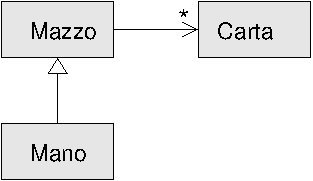
\includegraphics[scale=0.8]{figs/class1.pdf}}
\caption{Diagramma di classe.}
\label{fig.class1}
\end{figure}


La freccia con un triangolo vuoto rappresenta la relazione IS-A: in questo caso indica che Mano eredita da Mazzo.

La freccia standard rappresenta la relazione HAS-A; in questo caso un Mazzo ha riferimenti agli oggetti Carta.
\index{molteplicità (nel diagramma di classe)}

L'asterisco ({\tt *}) vicino alla testa della freccia indica una
{\bf molteplicità}, cioè quante Carte ha un Mazzo. Una molteplicità può essere un numero semplice, come {\tt 52}, un intervallo come {\tt 5..7}, o un asterisco che indica che un Mazzo può contenere un numero qualsiasi di Carte.

In questo diagramma non vi sono dipendenze. In genere, verrebbero illustrate con delle frecce tratteggiate. Se vi sono parecchie dipendenze, talvolta vengono omesse.

Un diagramma più dettagliato dovrebbe evidenziare che un Mazzo contiene in realtà una {\em lista} di Carte, ma i tipi predefiniti come liste e dizionari di solito non vengono inclusi in questi diagrammi.


\section{Debug}
\index{debug}

L'ereditarietà può rendere il debug difficoltoso, perché quando invocate un metodo su un oggetto, può risultare laborioso capire esattamente quale sia il metodo che viene invocato.
\index{ereditarietà}

Supponiamo che stiate scrivendo una funzione che lavori su oggetti Mano. Vorreste che fosse valida per Mani di tutti i tipi come ManiDiPoker, ManiDiBridge ecc. Se invocate un metodo come
{\tt mescola}, potrebbe essere quello definito in {\tt Mazzo},
ma se qualcuna delle sottoclassi sovrascrive il metodo, avrete invece quella diversa versione. Questo comportamento è appropriato, ma a volte può confondere.

Quando siete incerti sul flusso di esecuzione del vostro programma, la soluzione più semplice è aggiungere istruzioni di stampa all'inizio di ogni metodo importante. Se {\tt Mazzo.mescola} stampa un messaggio come {\tt Sto eseguendo Mazzo.mescola}, allora il programma traccia il flusso di esecuzione mentre viene eseguito.
\index{flusso di esecuzione}

In alternativa, potete usare la funzione seguente, che richiede un oggetto e un nome di metodo (come stringa) e restituisce la classe che contiene la definizione del metodo:

\begin{verbatim}
def trova_classe_def(obj, nome_metodo):
    for ty in type(obj).mro():
        if nome_metodo in ty.__dict__:
            return ty
\end{verbatim}
%
Ecco un esempio:

\begin{verbatim}
>>> mano = Mano()
>>> trova_classe_def(mano, 'mescola')
<class 'Carta.Mazzo'>
\end{verbatim}
%
Quindi il metodo {\tt mescola} di questa Mano è quello definito in{\tt Mazzo}.
\index{mro, metodo}
\index{metodo!mro}
\index{ordine di risoluzione dei metodi}

\verb"trova_classe_def" usa il metodo {\tt mro} per ricavare la lista degli oggetti classe (tipi) in cui verrà effettuata la ricerca dei metodi.  ``MRO'' sta per {\em Method Resolution Order} (ordine di risoluzione dei metodi), che è la sequenza di classi che Python ricerca per ``risolvere'' un nome di metodo.

Un consiglio per la progettazione di un programma: quando sovrascrivete un metodo, l'interfaccia del nuovo metodo dovrebbe essere la stessa di quello sostituito: deve richiedere gli stessi parametri, restituire lo stesso tipo, rispettare le stesse precondizioni e postcondizioni. Se rispettate questa regola, vedrete che ogni funzione progettata per un'istanza di una superclasse, come Mazzo, funzionerà anche con le istanze delle sottoclassi come Mano e ManoDiPoker.
\index{sovrascrittura}
\index{interfaccia}
\index{precondizione}
\index{postcondizione}

Se violate questa regola, conosciuta come ``principio di sostituzione di Liskov'', il vostro codice crollerà come (perdonatemi) un castello di carte.
\index{Liskov, principio di sostituzione}

\section{Incapsulamento dei dati}

Il capitolo precedente ha illustrato una tecnica di sviluppo detta
``progettazione orientata agli oggetti''.  Abbiamo identificato gli oggetti che ci servivano---come {\tt Tempo}, {\tt Punto} e {\tt Rettangolo}---e definito le classi per rappresentarli. Per ciascuno c'è un'evidente corrispondenza tra l'oggetto e una qualche entità del mondo reale (o per lo meno del mondo della matematica).
\index{tecnica di sviluppo!incapsulamento dei dati}

Ma altre volte la scelta degli oggetti e del modo in cui interagiscono è meno ovvia. In questo caso serve una tecnica di sviluppo diversa. Nella stessa maniera in cui abbiamo scoperto le interfacce delle funzioni per mezzo dell'incapsulamento e della generalizzazione, scopriamo ora le interfacce delle classi tramite l'{\bf incapsulamento dei dati}.
\index{incapsulamento!dei dati}

L'analisi di Markov, vista nel Paragrafo~\ref{markov}, è un buon esempio. Se scaricate il mio codice dal sito \url{http://thinkpython2.com/code/markov.py}, vi accorgerete che usa due variabili globali---\verb"suffix_map" e \verb"prefix"---che vengono lette e scritte da più funzioni.

\begin{verbatim}
suffix_map = {}        
prefix = ()            
\end{verbatim}

Siccome queste variabili sono globali, possiamo eseguire una sola analisi alla volta. Se leggessimo due testi contemporaneamente, i loro prefissi e suffissi verrebbero aggiunti nella stessa struttura di dati (il che produce comunque alcuni interessanti testi generati).

Per eseguire analisi multiple mantenendole separate, possiamo incapsulare lo stato di ciascuna analisi in un oggetto. Ecco come si presenta:

\begin{verbatim}
class Markov:

    def __init__(self):
        self.suffix_map = {}
        self.prefix = ()    
\end{verbatim}

Poi, trasformiamo le funzioni in metodi. Ecco per esempio \verb"elabora_parola":

\begin{verbatim}
    def elabora_parola(self, parola, ordine=2):
        if len(self.prefix) < ordine:
            self.prefix += (parola,)
            return

        try:
            self.suffix_map[self.prefix].append(parola)
        except KeyError:
            # se non c'e' una voce per questo prefisso, creane una
            self.suffix_map[self.prefix] = [parola]

        self.prefix = shift(self.prefix, parola)        
\end{verbatim}

Questa trasformazione di un programma---cambiarne la forma senza cambiarne il comportamento---è un altro esempio di refactoring (vedi Paragrafo~\ref{refactoring}).
\index{refactoring}

L'esempio suggerisce una tecnica di sviluppo per progettare oggetti e metodi:

\begin{enumerate}

\item Cominciare scrivendo funzioni che leggono e scrivono variabili globali (dove necessario)

\item Una volta ottenuto un programma funzionante, cercare le associazioni tra le variabili globali e le funzioni che le usano.

\item Incapsulare le variabili correlate come attributi di un oggetto.

\item Trasformare le funzioni associate in metodi della nuova classe.

\end{enumerate}

Come esercizio, scaricate il mio codice da
(\url{http://thinkpython2.com/code/markov.py}), e seguite i passi appena descritti per incapsulare le varibili globali come attributi di una nuova classe chiamata {\tt Markov}.  Soluzione: \url{http://thinkpython2.com/code/Markov.py} (notare la M maiuscola).


\section{Glossario}

\begin{description}

\item[codificare:]  Rappresentare un insieme di valori usando un altro insieme di valori e costruendo una mappatura tra di essi.
\index{codificare}

\item[attributo di classe:] Attributo associato ad un oggetto classe. Gli attributi di classe sono definiti all'interno di una definizione di classe ma esternamente ad ogni metodo.
\index{classe!attributo di}
\index{attributo!di classe}

\item[attributo di istanza:] Attributo associato ad un'istanza di una classe.
\index{istanza!attributo di}
\index{attributo!di istanza}

\item[impiallacciatura:] Metodo o funzione che fornisce un'interfaccia diversa a un'altra funzione, senza effettuare ulteriori calcoli.
\index{impiallacciatura}

\item[ereditarietà:] Capacità di definire una classe come versione modificata di una classe già definita in precedenza.
\index{ereditarietà}

\item[classe madre o superclasse:] Classe dalla quale una classe figlia eredita.
\index{classe!madre}

\item[classe figlia o sottoclasse:] Nuova classe creata ereditando da una classe esistente.
\index{classe!figlia}

\item[relazione IS-A:] Relazione tra una classe figlia e la sua classe madre.
\index{IS-A, relazione}

\item[relazione HAS-A:] Relazione tra due classi dove le istanze di una classe contengono riferimenti alle istanze dell'altra classe.
\index{HAS-A, relazione}

\item[dipendenza:] Relazione tra due classi dove istanze di una classe utilizzano istanze dell'altra classe, ma senza conservarle sotto forma di attributi.
\index{dipendenza, relazione}

\item[diagramma di classe:] Diagramma che illustra le classi di un programma e le relazioni tra di esse.
\index{diagramma!di classe}

\item[molteplicità:] Notazione in un diagramma di classe che mostra, per una relazione HAS-A, quanti riferimenti ad istanze di un'altra classe ci sono.
\index{molteplicità (nel diagramma di classe)}

\item[incapsulamento dei dati:] Tecnica di sviluppo che prevede un prototipo che usa variabili globali e una versione finale in cui le variabili globali vengono trasformate in attributi di istanza.
\index{incapsulamento!dei dati}
\index{tecnica di sviluppo!incapsulamento dei dati}

\end{description}

\newpage
\section{Esercizi}

\begin{exercise}
Dato il seguente programma, disegnate un diagramma di classe UML ({\em Unified Modeling Language}) che illustri queste classi e le relazioni che intercorrono tra esse.

\begin{verbatim}
class PingPongMadre:
    pass

class Ping(PingPongMadre):
    def __init__(self, pong):
        self.pong = pong


class Pong(PingPongMadre):
    def __init__(self, pings=None):
        if pings is None:
            self.pings = []
        else:
            self.pings = pings

    def add_ping(self, ping):
        self.pings.append(ping)

pong = Pong()
ping = Ping(pong)
pong.add_ping(ping)
\end{verbatim}


\end{exercise}

\vspace{0.2in}
\begin{exercise}

Scrivete un metodo per Mazzo di nome \verb"dai_mani" che prenda come parametri il numero di mani e il numero di carte da dare a ciascuna mano, e crei il numero stabilito di oggetti Mano, distribuisca il numero prefissato di carte a ogni mano e restituisca una lista delle Mani.

\end{exercise}

\vspace{0.2in}
\begin{exercise}
\label{poker}

Quelle che seguono sono le possibili combinazioni nel gioco del poker, in ordine crescente di valore e decrescente di probabilità:
\index{poker}

\begin{description}

\item[coppia:] due carte dello stesso valore
\vspace{-0.05in}

\item[doppia coppia:] due coppie di carte dello stesso valore
\vspace{-0.05in}

\item[tris:] tre carte dello stesso valore
\vspace{-0.05in}

\item[scala:] cinque carte con valori in sequenza (gli assi possono essere sia la carta di valore inferiore che quella di valore superiore, per cui {\tt Asso-2-3-4-5} è una scala, e anche {\tt 10-Fante-Regina-Re-Asso}, ma non {\tt Regina-Re-Asso-2-3}).
\vspace{-0.05in}

\item[colore:] cinque carte dello stesso seme
\vspace{-0.05in}

\item[full:] tre carte dello stesso valore più una coppia di carte dello stesso valore
\vspace{-0.05in}

\item[poker:] quattro carte dello stesso valore
\vspace{-0.05in}

\item[scala reale:] cinque carte dello stesso seme in scala (definita come sopra)
\vspace{-0.05in}

\end{description}
%
Scopo di questo esercizio è stimare la probabilità di avere servita una di queste combinazioni.

\begin{enumerate}

\item Scaricate i file seguenti da \url{http://thinkpython2.com/code}:

\begin{description}

\item[{\tt Card.py}]: Versione completa delle classi {\tt Carta},
{\tt Mazzo} e {\tt Mano} di questo capitolo.

\item[{\tt PokerHand.py}]: Implementazione incompleta di una classe che rappresenta una mano di poker con del codice di prova.


\end{description}
%
\item Se eseguite {\tt PokerHand.py}, serve delle mani di sette carte e controlla se qualcuna contenga un colore. Leggete attentamente il codice prima di proseguire.

\item Aggiungete dei metodi a {\tt PokerHand.py} di nome \verb"ha_coppia",
\verb"ha_doppiacoppia", ecc. che restituiscano True o False a seconda che le mani soddisfino o meno il rispettivo criterio. Il codice deve funzionare indipendentemente dal numero di carte che contiene la mano (5 e 7 carte sono i casi più comuni).

\item Scrivete un metodo di nome {\tt classifica} che riconosca la combinazione più elevata in una mano e imposta di conseguenza l'attributo
{\tt label}.  Per esempio, una mano di 7 carte può contenere un colore e una coppia; deve essere etichettata ``colore''.

\item Quando siete sicuri che i vostri metodi di classificazione funzionano, il passo successivo è stimare la probabilità delle varie mani. Scrivete una funzione in {\tt PokerHand.py} che mescoli un mazzo di carte, lo divida in mani, le classifichi e conti quante volte compare ciascuna combinazione.

\item Stampate una tabella delle combinazioni con le rispettive probabilità. Eseguite il vostro programma con numeri sempre più grandi di mani finché i valori ottenuti convergono ad un ragionevole grado di accuratezza. Confrontate i vostri risultati con i valori pubblicati su \url{http://en.wikipedia.org/wiki/Hand_rankings}.

\end{enumerate}

Soluzione: \url{http://thinkpython2.com/code/PokerHandSoln.py}.
\end{exercise}


\chapter{Ulteriori strumenti}

Uno degli obiettivi di questo libro è di illustrarvi il minimo indispensabile di Python. Quando esistono due modi diversi di fare qualcosa, preferisco sceglierne uno ed evitare di citare l'altro, oppure inserire il secondo all'interno di un esercizio.

Ora vorrei tornare a recuperare alcune chicche che avevo tralasciato. Python è dotato di parecchie funzionalità che non sono indispensabili---potete scrivere del buon codice anche senza usarle---ma che in certi casi vi permettono di scrivere del codice più conciso, leggibile, efficiente, o anche tutte e tre le cose insieme.

% TODO: add the with statement

\section{Espressioni condizionali}

Abbiamo visto nel Paragrafo~\ref{conditional.execution} le istruzioni condizionali, che vengono usate di frequente per scegliere uno tra due valori alternativi, per esempio:
\index{condizionale, espressione}
\index{espressione!condizionale}

\begin{verbatim}
if x > 0:
    y = math.log(x)
else:
    y = float('nan')
\end{verbatim}

Questa istruzione controlla se {\tt x} è positivo. Se lo è, calcola
{\tt math.log}, altrimenti {\tt math.log} scatenerebbe un ValueError.  Per evitare che il programma si arresti, generiamo un ``NaN'', che è un valore a virgola mobile speciale che rappresenta ``Not a Number'' (Non è un Numero).
\index{NaN}
\index{floating-point}

Possiamo scrivere questa condizione in modo più conciso utilizzando un'{\bf espressione condizionale}:

\begin{verbatim}
y = math.log(x) if x > 0 else float('nan')
\end{verbatim}

Si può quasi leggere questa riga come fosse: ``{\tt y} diventa log-{\tt x}
se {\tt x} è maggiore di 0; altrimenti diventa NaN''.

A volte, le funzioni ricorsive possono essere riscritte utilizzando le espressioni  condizionali. Prendiamo ad esempio una versione ricorsiva di {\tt fattoriale}:
\index{fattoriale}
\index{funzione!fattoriale}

\begin{verbatim}
def fattoriale(n):
    if n == 0:
        return 1
    else:
        return n * fattoriale(n-1)
\end{verbatim}

Si può riscrivere così:

\begin{verbatim}
def fattoriale(n):
    return 1 if n == 0 else n * fattoriale(n-1)
\end{verbatim}

Un altro utilizzo delle espressioni condizionali è la gestione degli argomenti opzionali. Per esempio, ecco il metodo init di
{\tt GoodKangaroo} (vedere Esercizio~\ref{kangaroo}):
\index{opzionale, argomento}
\index{argomento!opzionale}

\begin{verbatim}
    def __init__(self, nome, contenuti=None):
        self.nome = nome
        if contenuti == None:
        contenuti = []
        self.contenuto_tasca = contenuti
\end{verbatim}

Si può riscrivere così:

\begin{verbatim}
    def __init__(self, nome, contenuti=None):
        self.nome = nome
        self.contenuto_tasca = [] if contenuti == None else contenuti 
\end{verbatim}

In generale, si può sostituire un'istruzione condizionale con un'espressione condizionale se entrambe le ramificazioni contengono semplici espressioni che vengono o ritornate o assegnate alla stessa variabile.
\index{condizionale, istruzione}
\index{istruzione!condizionale}



\section{List comprehension}

Nel Paragrafo~\ref{filter} abbiamo visto gli schemi di mappa e filtro. Per esempio, questa funzione prende una lista di stringhe, mappa il metodo delle stringhe {\tt capitalize} negli elementi e restituisce una nuova lista di stringhe:

\begin{verbatim}
def tutte_maiuscole(t):
    res = []
    for s in t:
        res.append(s.capitalize())
    return res
\end{verbatim}

Si può scrivere in modo più conciso utilizzando una {\bf list comprehension}:
\index{list comprehension}

\begin{verbatim}
def tutte_maiuscole(t):
    return [s.capitalize() for s in t]
\end{verbatim}

Gli operatori parentesi quadre indicano che stiamo costruendo una nuova lista. L'espressione all'interno delle parentesi specifica gli elementi della lista, e il costrutto {\tt for} specifica la sequenza che stiamo attraversando.
\index{lista}
\index{for, ciclo}

La sintassi di una list comprehension è un po' sgraziata, perché la variabile del ciclo, {\tt s} in questo esempio, compare nell'espressione prima di ottenerne la definizione.
\index{loop variable}

Si può usare la list comprehension anche per filtrare. Per esempio, questa funzione seleziona solo gli elementi di {\tt t} che sono composti di lettere maiuscole, e restituisce una nuova lista:
\index{filtro, schema}
\index{schema!filtro}

\begin{verbatim}
def solo_maiuscole(t):
    res = []
    for s in t:
        if s.isupper():
            res.append(s)
    return res
\end{verbatim}

Riscriviamola usando una list comprehension:

\begin{verbatim}
def solo_maiuscole(t):
    return [s for s in t if s.isupper()]
\end{verbatim}

Le list comprehension sono concise e leggibili, almeno per le espressioni semplici. E di solito sono più veloci dei cicli \verb'for' equivalenti, a volte molto più veloci. Capisco quindi se mi state biasimando per non avervene parlato prima.

La giustificazione è che il debug delle list comprehension è più difficile, perché non potete inserire delle istruzioni di stampa nel ciclo. Vi consiglio di usarle solo se i calcoli sono abbastanza semplici da avere buone probabilità di azzeccarci al primo colpo. Che per un principiante, vuol dire quasi mai.
\index{debug}


\section{Generator expression}

Le {\bf generator expression} assomigliano sintatticamente a delle list comprehension, ma con parentesi tonde anziché quadre:
\index{generator expression}

\begin{verbatim}
>>> g = (x**2 for x in range(5))
>>> g
<generator object <genexpr> at 0x7f4c45a786c0>
\end{verbatim}
%
Il risultato è un oggetto generatore che è in grado di iterare attraverso una sequenza di valori. Ma a differenza di una list comprehension, non calcola i valori tutti in una volta: attende che gli venga chiesto di farlo.
Con la funzione predefinita {\tt next}, si ottiene dal generatore il valore successivo:
\index{generatore, oggetto}
\index{oggetto!generatore}

\begin{verbatim}
>>> next(g)
0
>>> next(g)
1
\end{verbatim}
%
Arrivati alla fine della sequenza, {\tt next} solleva un'eccezione
StopIteration.  Si può anche usare un ciclo {\tt for} per iterare attraverso i valori:
\index{StopIteration}
\index{eccezione!StopIteration}

\begin{verbatim}
>>> for val in g:
...     print(val)
4
9
16
\end{verbatim}
%
L'oggetto generatore mantiene traccia del punto in cui si trova all'interno della sequenza, quindi il ciclo {\tt for} riprende da dove {\tt next} era rimasto. Una volta che il generatore è esaurito, continua sollevando delle {\tt StopIteration}:

\begin{verbatim}
>>> next(g)
StopIteration
\end{verbatim}

Le generator expression vengono usate spesso con funzioni come {\tt sum},
{\tt max}, e {\tt min}:
\index{sum, funzione}
\index{funzione!sum}

\begin{verbatim}
>>> sum(x**2 for x in range(5))
30
\end{verbatim}


\section{{\tt any} e {\tt all}}

Python dispone di una funzione predefinita di nome {\tt any}, che prende una sequenza di valori booleani e restituisce {\tt True} se almeno uno dei valori è {\tt True}.  Funziona sulle liste:
\index{any, funzione}
\index{funzione!any}

\begin{verbatim}
>>> any([False, False, True])
True
\end{verbatim}
%
Ma viene usata spesso con le generator expression:
\index{generator expression}

\begin{verbatim}
>>> any(lettera == 't' for lettera in 'monty')
True
\end{verbatim}
%
Questo esempio non è granché utile, perché fa la stessa cosa dell'operatore {\tt in}.  Ma possiamo usare {\tt any} per riscrivere alcune delle funzioni di ricerca che avevamo scritto nel Paragrafo~\ref{search}.  Per esempio, avremmo potuto scrivere {\tt evita} così:
\index{schema di ricerca}
\index{ricerca!schema}

\begin{verbatim}
def evita(parola, vietate):
    return not any(lettera in vietate for lettera in parola)
\end{verbatim}
%
La funzione si legge quasi come fosse: ``la {\tt parola} evita le
{\tt vietate} se non c'è alcuna lettera in {\tt vietate} per ogni lettera in {\tt parola}.''

L'uso di {\tt any} con una generator expression è efficiente, perché si ferma immediatamente se trova un valore {\tt True}, senza dover necessariamente verificare tutta la sequenza. 

Python contiene poi un'altra funzione predefinita, {\tt all}, che restituisce
{\tt True} se ogni elemento di una sequenza è {\tt True}.  Come esercizio, usate {\tt all} per riscrivere la funzione \verb"usa_tutte" del Paragrafo~\ref{search}.
\index{all, funzione}
\index{funzione!all}


\section{Insiemi (set)}
\label{sets}

Nel Paragrafo~\ref{dictsub} avevo utilizzato dei dizionari per trovare le parole che comparivano in un testo, ma non in un elenco di parole. La funzione che avevo scritto prendeva {\tt d1}, contenente le parole del testo come chiavi, e {\tt d2}, contenente l'elenco di parole. Essa restituiva un dizionario contenente le chiavi di {\tt d1} che non comparivano in {\tt d2}.

\begin{verbatim}
def sottrai(d1, d2):
    res = dict()
    for chiave in d1:
        if chiave not in d2:
            res[chiave] = None
    return res
\end{verbatim}
%
In tutti questi dizionari, i valori sono {\tt None} perché non sono necessari e non vengono usati. Ma questo spreca dello spazio di memoria.
\index{sottrazione!di dizionari}

Python dispone di un altro tipo predefinito chiamato {\bf insieme} o {\tt set}, che si comporta come una raccolta di chiavi di dizionario prive di valori. Aggiungere elementi ad un insieme è rapido, come pure controllare se un elemento appartiene all'insieme. Vengono poi forniti metodi e operatori per eseguire le comuni operazioni sugli insiemi.
\index{insieme}
\index{oggetto!set}

Per esempio, la sottrazione di insiemi è disponibile sotto forma di metodo chiamato {\tt difference} oppure come operatore, {\tt -}.  Possiamo allora riscrivere {\tt sottrai} in questo modo:
\index{sottrazione!di insiemi}

\begin{verbatim}
def sottrai(d1, d2):
    return set(d1) - set(d2)
\end{verbatim}
%
Il risultato è un insieme anziché un dizionario, ma per operazioni come l'iterazione il comportamento è identico. 

Alcuni esercizi di questo libro possono essere svolti in modo conciso ed efficiente usando gli insiemi.  Per esempio, questa è una soluzione di
\verb"ha_duplicati", dall'Esercizio~\ref{duplicate}, che utilizza un dizionario:

\begin{verbatim}
def ha_duplicati(t):
    d = {}
    for x in t:
        if x in d:
            return True
        d[x] = True
    return False
\end{verbatim}

Quando un elemento compare per la prima volta, viene aggiunto al dizionario. Se il medesimo elemento ricompare, la funzione restituisce {\tt True}.

Usando gli insiemi, si può riscrivere la funzione così:

\begin{verbatim}
def ha_duplicati(t):
    return len(set(t)) < len(t)
\end{verbatim}
%
Siccome un elemento può comparire in un insieme solo una volta, se in {\tt t} esiste qualche elemento che compare più volte, l'insieme risulterà più piccolo di {\tt t}. Se invece non ci sono duplicati, l'insieme avrà la stessa dimensione di {\tt t}.
\index{duplicato}

Si possono usare gli insiemi anche per risolvere alcuni esercizi del Capitolo~\ref{wordplay}.  Per esempio, questa è la versione di
\verb"usa_solo" con un ciclo:

\begin{verbatim}
def usa_solo(parola, valide):
    for lettera in parola: 
        if lettera not in valide:
            return False
    return True
\end{verbatim}
%
\verb"usa_solo" controlla se tutte le lettere in una {\tt word} sono tra quelle {\tt valide}.  La possiamo riscrivere così:

\begin{verbatim}
def usa_solo(parola, valide):
    return set(parola) <= set(valide)
\end{verbatim}
%
L'operatore \verb"<=" controlla se un insieme è un sottoinsieme di un altro, compresa la possibilità che siano uguali, il che è vero se tutte le lettere nella {\tt parola} fanno parte delle {\tt valide}.
\index{sottoinsieme}

Per esercizio, riscrivete la funzione \verb"evita" usando gli insiemi.


\section{Contatori}

Un contatore è una specie di insieme, tranne per il fatto che se un elemento compare più di una volta, il contatore prende nota di quante volte compare. Se vi è noto il concetto matematico di {\bf multiinsieme}, un contatore è un modo immediato per rappresentarlo.
\index{contatore}
\index{oggetto!Counter}
\index{multiinsieme}

Il contatore è definito all'interno di un modulo standard chiamato {\tt collections}, quindi dovete innanzitutto importarlo. Potete inizializzare un contatore con una stringa, lista o qualsiasi altro oggetto che sia iterabile:
\index{collections}
\index{modulo!collections}

\begin{verbatim}
>>> from collections import Counter
>>> conta = Counter('parrot')
>>> conta
Counter({'r': 2, 't': 1, 'o': 1, 'p': 1, 'a': 1})
\end{verbatim}

I contatori si comportano per molti versi come i dizionari: fanno corrispondere ciascuna chiave al numero di volte in cui essa compare. Come per i dizionari, le chiavi devono essere idonee all'hashing.

A differenza dei dizionari, i contatori non sollevano eccezioni in caso di accesso a un elemento che non esiste; invece, restituiscono 0:

\begin{verbatim}
>>> conta['d']
0
\end{verbatim}

Possiamo usare i contatori per riscrivere \verb"anagramma" dell'Esercizio~\ref{anagram}:

\begin{verbatim}
def anagramma(parola1, parola2):
    return Counter(parola1) == Counter(parola2)
\end{verbatim}

Se due parole sono anagrammi, contengono le stesse lettere, lo stesso numero di volte: pertanto i loro contatori sono equivalenti.

Anche i contatori sono dotati dei metodi e degli operatori per eseguire le operazioni tipiche degli insiemi, incluse addizione, sottrazione e intersezione.  Ed espongono un metodo molto utile, \verb"most_common", che
restituisce una lista di coppie valore-frequenza, in ordine di frequenza decrescente:

\begin{verbatim}
>>> conta = Counter('parrot')
>>> for valore, frequenza in count.most_common(3):
...     print(valore, frequenza)
r 2
p 1
a 1
\end{verbatim}


\section{defaultdict}

Il modulo {\tt collections} contiene anche {\tt defaultdict}, che è simile a un dizionario, con la differenza che quando si tenta di accedere ad una chiave inesistente, può generare al volo un nuovo valore.
\index{defaultdict}
\index{oggetto!defaultdict}
\index{collections}
\index{modulo!collections}

Nel creare un defaultdict, dovete fornire una funzione che viene usata per creare i nuovi valori. Una funzione usata per creare oggetti viene detta da alcuni {\bf factory}. Le funzioni predefinite che creano liste, insiemi e altri tipi, possono essere usate come factory:
\index{factory, funzione}

\begin{verbatim}
>>> from collections import defaultdict
>>> d = defaultdict(list)
\end{verbatim}

Notate che l'argomento è {\tt list}, che è un oggetto classe, non {\tt list()}, che è una nuova lista. La funzione che avete creato viene chiamata soltanto quando tentate di accedere ad una chiave che non esiste.

\begin{verbatim}
>>> t = d['nuova chiave']
>>> t
[]
\end{verbatim}

La nuova lista, che chiamiamo {\tt t}, viene aggiunta al dizionario. Quindi se modifichiamo {\tt t}, i cambiamenti compaiono in {\tt d}:

\begin{verbatim}
>>> t.append('nuovo valore')
>>> d
defaultdict(<class 'list'>, {'nuova chiave': ['nuovo valore']})
\end{verbatim}

Se state creando un dizionario di liste, usare {\tt defaultdict} permette spesso di scrivere codice più semplice. Nella mia risoluzione dell'Esercizio~\ref{anagrams}, che potete scaricare da
\url{http://thinkpython2.com/code/anagram_sets.py}, ho creato un dizionario che mappa da una stringa ordinata di lettere nella lista di parole che si possono comporre con quelle lettere. Per esempio, {\tt 'opst'} corrisponde alla lista {\tt ['opts', 'post', 'pots', 'spot', 'stop', 'tops']}.

Questo è il codice di partenza:

\begin{verbatim}
def tutti_anagrammi(nomefile):
    d = {}
    for riga in open(nomefile):
        parola = riga.strip().lower()
        t = signature(parola)
        if t not in d:
            d[t] = [parola]
        else:
            d[t].append(parola)
    return d
\end{verbatim}

Si può semplificare usando {\tt setdefault}, che potreste avere usato nell'Esercizio~\ref{setdefault}:
\index{setdefault}

\begin{verbatim}
def tutti_anagrammi(nomefile):
    d = {}
    for riga in open(nomefile):
        parola = riga.strip().lower()
        t = signature(parola)
        d.setdefault(t, []).append(parola)
    return d
\end{verbatim}

Questa soluzione ha il difetto di creare ogni volta una nuova lista, anche se non è necessario. Non è un grande problema se si tratta di liste, ma se la funzione factory è complessa, può diventarlo.
\index{factory, funzione}

Ma si può evitare il problema e semplificare il codice con un {\tt defaultdict}:

\begin{verbatim}
def tutti_anagrammi(nomefile):
    d = defaultdict(list)
    for riga in open(nomefile):
        parola = riga.strip().lower()
        t = signature(parola)
        d[t].append(parola)
    return d
\end{verbatim}

La mia risoluzione dell'Esercizio~\ref{poker}, scaricabile da
\url{http://thinkpython2.com/code/PokerHandSoln.py},
usa {\tt setdefault} nella funzione
\verb"has_straightflush".  Ha il difetto di creare un oggetto {\tt Mano} ad ogni ripetizione del ciclo, anche se non serve. Come esercizio, riscrivetela usando un defaultdict.


\section{Tuple con nome (namedtuple)}

Molti oggetti semplici sono, fondamentalmente, delle raccolte di valori tra loro correlati. Ad esempio, l'oggetto Punto che abbiamo definito nel Capitolo~\ref{clobjects} contiene due numeri, {\tt x} e {\tt y}.  Nella definizione di una classe come questa, si comincia di solito con un metodo init e un metodo str:

\begin{verbatim}
class Punto:

    def __init__(self, x=0, y=0):
        self.x = x
        self.y = y

    def __str__(self):
        return '(%g, %g)' % (self.x, self.y)
\end{verbatim}

Qui serve molto codice per trasportare una piccola quantità di informazione. Python dispone di un modo più conciso per dire la stessa cosa:

\begin{verbatim}
from collections import namedtuple
Punto = namedtuple('Punto', ['x', 'y'])
\end{verbatim}

Il primo argomento è il nome della classe che volete creare. Il secondo è una lista degli attributi, come stringhe, che l'oggetto Punto deve avere. Il valore di ritorno da {\tt namedtuple} è un oggetto classe:
\index{namedtuple}
\index{tupla!con nome}
\index{oggetto!namedtuple}
\index{collections}
\index{modulo!collections}

\begin{verbatim}
>>> Punto
<class '__main__.Punto'>
\end{verbatim}

{\tt Punto} dispone automaticamente dei metodi \verb"__init__" e
\verb"__str__", pertanto non occorre scriverli.
\index{classe, oggetto}
\index{oggetto!classe}

Per creare un oggetto Punto, usate la classe Punto come fosse una funzione:

\begin{verbatim}
>>> p = Punto(1, 2)
>>> p
Punto(x=1, y=2)
\end{verbatim}

Il metodo init assegna gli argomenti agli attributi usando i nomi che avete specificato. Il metodo str mostra una rappresentazione dell'oggetto Punto e dei suoi attributi. 

Potete accedere agli elementi della namedtuple usando il loro nome:

\begin{verbatim}
>>> p.x, p.y
(1, 2)
\end{verbatim}

Ma potete anche trattare una namedtuple come una tupla, e usare gli indici:

\begin{verbatim}
>>> p[0], p[1]
(1, 2)

>>> x, y = p
>>> x, y
(1, 2)
\end{verbatim}

Le tuple con nome offrono un modo rapido per definire delle classi semplici.
Per contro, le classi semplici non sempre rimangono tali. Si potrebbe decidere in un secondo tempo di voler aggiungere dei metodi a una tupla con nome. In quel caso, occorrerebbe definire una nuova classe che erediti dalla tupla con nome:
\index{ereditarietà}

\begin{verbatim}
class IperPunto(Punto):
    # aggiungere qui altri metodi
\end{verbatim}

Oppure si può passare ad una definizione di classe tradizionale.


\section{Raccolta di argomenti con nome}

Nel Paragrafo~\ref{gather}, avevamo visto come scrivere una funzione che raccoglie in una tupla i suoi argomenti:
\index{raccolta}

\begin{verbatim}
def stampatutti(*args):
    print(args)
\end{verbatim}
%
Questa funzione può essere chiamata con un numero qualunque di argomenti posizionali (cioè, argomenti che non hanno nome):
\index{posizionale, argomento}
\index{argomento!posizionale}

\begin{verbatim}
>>> stampatutti(1, 2.0, '3')
(1, 2.0, '3')
\end{verbatim}
%
Tuttavia, l'operatore di raccolta {\tt *} non funziona con gli argomenti con nome:
\index{argomento!con nome}

\begin{verbatim}
>>> stampatutti(1, 2.0, terzo='3')
TypeError: stampatutti() got an unexpected keyword argument 'terzo'
\end{verbatim}
%
Per raccogliere gli argomenti con nome, si usa invece l'operatore {\tt **}:

\begin{verbatim}
def stampatutti(*args, **kwargs):
    print(args, kwargs)
\end{verbatim}
%
Si può chiamare il parametro di raccolta come si vuole, ma per prassi si usa
{\tt kwargs}.  Il risultato è un dizionario che mappa i nomi nei valori:

\begin{verbatim}
>>> stampatutti(1, 2.0, terzo='3')
(1, 2.0) {'terzo': '3'}
\end{verbatim}
%
Se disponete di un dizionario di nomi e valori, potete usare l'operatore di spacchettamento, {\tt **} , per chiamare una funzione:
\index{spacchettamento}

\begin{verbatim}
>>> d = dict(x=1, y=2)
>>> Punto(**d)
Punto(x=1, y=2)
\end{verbatim}
%
Senza l'operatore di spacchettamento, la funzione interpreterebbe {\tt d} come un singolo argomento posizionale, assegnandolo a {\tt x} e lamentando l'assenza di qualcosa da assegnare a {\tt y}:

\begin{verbatim}
>>> d = dict(x=1, y=2)
>>> Punto(d)
Traceback (most recent call last):
  File "<stdin>", line 1, in <module>
TypeError: __new__() missing 1 required positional argument: 'y'
\end{verbatim}
%
Quando si lavora con funzioni che hanno parecchi parametri, è una buona idea creare e passare loro dei dizionari che contengono le opzioni di uso più frequente.


\section{Glossario}

\begin{description}

\item[espressione condizionale:] Un'espressione che contiene uno tra due alternativi valori, a seconda di una data condizione.
\index{condizionale, espressione}
\index{espressione!condizionale}

\item[list comprehension:] Espressione con un ciclo {\tt for} tra parentesi quadre che genera una nuova lista.
\index{list comprehension}

\item[generator expression:] Espressione con un ciclo {\tt for} tra parentesi tonde che produce un oggetto generatore.  
\index{generator expression}

\item[multiinsieme:] Ente matematico che rappresenta una corrispondenza tra gli elementi di un insieme e il numero di volte in cui compaiono. 

\item[factory:] Funzione, di solito passata come argomento, usata per creare oggetti.
\index{factory, funzione}

\end{description}


\section{Esercizi}

\begin{exercise}

La seguente funzione calcola ricorsivamente il coefficiente binomiale:

\begin{verbatim}
def coeff_binomiale(n, k):
    """Calcola il coefficiente binomiale "n sopra k".

    n: numero di prove
    k: numero di successi

    ritorna: int
    """
    if k == 0:
        return 1
    if n == 0:
        return 0

    res = coeff_binomiale(n-1, k) + coeff_binomiale(n-1, k-1)
    return res
\end{verbatim}

Riscrivete il corpo della funzione usando delle espressioni condizionali nidificate.

Nota: questa funzione non è molto efficiente, perché finisce per calcolare continuamente gli stessi valori. Potreste renderla più efficiente con la memoizzazione (vedere Paragrafo~\ref{memoize}). Riscontrerete però che è difficile farlo, scrivendola con le espressioni condizionali.

\end{exercise}


\appendix

\chapter{Debug}

\index{debug}
Nell'operazione di rimozione degli errori da un programma, è opportuno distinguere i vari tipi di errore in modo da poterli rintracciare più velocemente:

\begin{itemize}

\item Gli errori di sintassi vengono scoperti dall'interprete quando traduce il codice sorgente in codice macchina. Indicano che c'è qualcosa di sbagliato nella struttura del programma. Esempio: omettere i due punti alla fine di una istruzione {\tt def} genera il messaggio, un po' ridondante, {\tt SyntaxError: invalid syntax}.
\index{sintassi!errore di}
\index{errore!di sintassi}

\item Gli errori di runtime sono prodotti dall'interprete se qualcosa va storto durante l'esecuzione del programma. Nella maggior parte dei casi, il messaggio di errore specifica dove si è verificato l'errore e quali funzioni erano in esecuzione. Esempio: una ricorsione infinita causa un errore di runtime ``{\tt maximum recursion depth exceeded}''.
\index{errore!in esecuzione}
\index{errore!di runtime}
\index{runtime!errore di}
\index{eccezione}

\item Gli errori di semantica sono dei problemi con un programma che viene eseguito senza produrre messaggi di errore, ma che non fa le cose nel modo giusto. Esempio: un'espressione può essere valutata secondo un ordine diverso da quello che si intendeva, generando un risultato non corretto.
\index{semantica!errore di}
\index{errore!di semantica}
\end{itemize}

La prima cosa da fare nel debug è capire con che tipo di errore abbiamo a che fare. Anche se i paragrafi che seguono sono organizzati per tipo di errore, alcune tecniche sono applicabili in più di una situazione.


\section{Errori di sintassi}
\index{errore!messaggio di}

Gli errori di sintassi sono in genere facili da sistemare, una volta capito in cosa consistono. Purtroppo, il messaggio di errore spesso è poco utile. Quelli più comuni sono: {\tt SyntaxError: invalid syntax} e
{\tt SyntaxError: invalid token}, nessuno dei quali è molto esplicativo.

In compenso, il messaggio comunica il punto del programma dove si è verificato il problema. Più precisamente, dice dove Python ha notato il problema, che non è necessariamente il punto in cui si trova l'errore.
A volte l'errore è prima del punto indicato dal messaggio, spesso nella riga precedente.
\index{sviluppo incrementale}
\index{tecnica di sviluppo!incrementale}

Se state costruendo il programma in modo incrementale, è molto probabile che l'errore sia nell'ultima riga che avete aggiunto.

Se state copiando il codice da un libro, cominciate confrontando attentamente il vostro codice con quello del libro. Controllate ogni carattere. Ricordate però che anche il libro può essere sbagliato, e se vedete qualcosa che somiglia a un errore di sintassi, potrebbe esserlo.

Ecco alcuni modi di evitare i più comuni errori di sintassi:
\index{sintassi}

\begin{enumerate}

\item Accertatevi di non usare parole chiave di Python come nomi di variabile.
\index{parola chiave}

\item Controllate che ci siano i due punti alla fine di ogni intestazione di tutte le istruzioni composte, inclusi {\tt for}, {\tt while},
{\tt if}, e le istruzioni {\tt def}.
\index{intestazione}
\index{due punti}

\item Accertatevi che ogni stringa nel codice sia racchiusa da una coppia di virgolette o apici, e che questi siano di tipo indifferenziato e non ``tipografici''.
\index{virgolette}

\item Se avete stringhe a righe multiple con triple virgolette, accertatevi di averle chiuse in modo appropriato. Una stringa non chiusa può causare un errore di {\tt invalid token} al termine del programma, oppure può trattare la parte che segue del programma come fosse una stringa, finché non incontra la stringa successiva. Nel secondo caso, potrebbe anche non produrre affatto un messaggio di errore!
\index{stringa!a righe multiple}

\item Un operatore di apertura non chiuso---\verb+(+, \verb+{+, o
  \verb+[+---fa sì che Python consideri la riga successiva come parte dell'istruzione corrente. In genere, si verifica un errore nella riga immediatamente successiva.

\item Controllate che non ci sia il classico {\tt =} al posto di {\tt ==} all'interno di un'istruzione condizionale.
\index{istruzione!condizionale}

\item Controllate l'indentazione per assicurarvi che il codice sia allineato nel modo corretto. Python può gestire sia spazi che tabulazioni, ma se li mescolate possono esserci problemi. Il modo migliore di evitarli è usare un editor di testo appositamente realizzato per Python, che gestisca l'indentazione in modo coerente.
\index{indentazione}
\index{spazi}

\item Se nel codice (compresi stringhe e commenti) ci sono caratteri non-ASCII, tipo le lettere accentate, potrebbero causare problemi, anche se Python 3 gestisce abbastanza bene questi caratteri. Fate attenzione, se copiate e incollate del testo da una pagina web o da altre fonti.

\end{enumerate}

Se nulla di tutto questo funziona, continuate con il paragrafo seguente...


\subsection{Continuo a fare modifiche ma non cambia nulla.}

Se l'interprete dice che c'è un errore ma non lo trovate, può essere che voi e l'interprete non stiate guardando lo stesso codice. Controllate il vostro ambiente di programmazione per assicurarvi che il programma che state modificando sia proprio quello che Python sta tentando di eseguire.

Se non ne siete certi, provate a mettere deliberatamente un evidente errore di sintassi all'inizio del programma e rieseguitelo. Se l'interprete non trova l'errore, non state eseguendo il nuovo codice.

Alcune cause possibili:

\begin{itemize}

\item Avete modificato il file e dimenticato di salvare le modifiche prima dell'esecuzione. Alcuni ambienti di programmazione lo fanno automaticamente, ma altri no.

\item Avete cambiato il nome del file, ma state eseguendo ancora quello con il vecchio nome.

\item Qualcosa nel vostro ambiente di sviluppo non è configurato correttamente.

\item Se state scrivendo un modulo usando {\tt import}, accertatevi di non dare al vostro modulo lo stesso nome di uno dei moduli standard di Python.

\item Se state usando {\tt import} per leggere un modulo, ricordatevi che dovete riavviare l'interprete o usare {\tt reload} per leggere un file modificato. Se importate nuovamente il modulo, non succederà nulla.
\index{modulo!reload}
\index{reload, funzione}
\index{funzione!reload}

\end{itemize}

Se vi bloccate e non riuscite a capire cosa sta succedendo, un'alternativa è ripartire con un nuovo programma come ``Ciao, mondo!'', e accertarvi di avere un programma ben conosciuto da eseguire. Quindi, aggiungete gradualmente i pezzi del programma originale a quello nuovo.


\section{Errori di runtime}

Una volta che il programma è sintatticamente corretto, Python può leggerlo e quantomeno cominciare ad eseguirlo. Cosa può succedere di spiacevole?


\subsection{Il programma non fa assolutamente nulla.}

È il problema più frequente se il vostro file consiste di funzioni e classi, ma in realtà non invoca alcuna funzione per avviare l'esecuzione. Può essere una cosa intenzionale, se intendete utilizzarlo solo come modulo da importare allo scopo di fornire le classi e le funzioni.

Se non è questo il caso, assicuratevi che nel programma ci sia una chiamata di funzione e che il flusso di esecuzione la raggiunga (vedete anche il paragrafo ``Flusso di esecuzione'' più avanti).


\subsection{Il programma si blocca.}
\index{ciclo!infinito}
\index{ricorsione!infinita}
\index{blocco}

Se un programma si blocca e pare che non stia succedendo nulla, spesso vuol dire che è incappato in un ciclo infinito o in una ricorsione infinita.

\begin{itemize}

\item Se c'è un ciclo particolare dove sospettate che stia il problema, aggiungete un'istruzione di stampa immediatamente prima del ciclo che dice:
``Sto entrando nel ciclo'' e una immediatamente dopo che dice:
``Sto uscendo dal ciclo''.

Avviate il programma. Se viene visualizzato il primo messaggio ma non il secondo, c'è un ciclo infinito. Proseguite con il Paragrafo ``Ciclo infinito'' più sotto.

\item Il più delle volte, in presenza di una ricorsione infinita, il programma funziona per qualche tempo per poi produrre un errore {\tt RuntimeError: Maximum
recursion depth exceeded}.  Se succede questo, andate al Paragrafo
``Ricorsione infinita''.

Se non ottenete questo errore ma sospettate che ci sia un problema con un metodo o funzione ricorsivi, potete usare ugualmente le tecniche illustrate nel Paragrafo ``Ricorsione infinita''.

\item Se nessuno di questi punti funziona, fate delle prove su altri cicli o funzioni e metodi ricorsivi.

\item Se ancora non funziona, forse non avete ben chiaro il flusso di esecuzione del vostro programma. Andate al relativo Paragrafo.

\end{itemize}


\subsubsection{Ciclo infinito}
\index{ciclo!infinito}
\index{condizione}
\index{ciclo!condizione}

Se sospettate che vi sia un ciclo infinito e di sapere quale ciclo in particolare stia causando il problema, aggiungete un'istruzione di stampa alla fine del ciclo in modo da visualizzare il valore delle variabili nella condizione e il valore della condizione.

Per esempio:

\begin{verbatim}
while x > 0 and y < 0 :
    # fa qualcosa con x
    # fa qualcosa con y

    print('x: ', x)
    print('y: ', y)
    print('condizione: ', (x > 0 and y < 0))
\end{verbatim}
%
Ora, eseguendo il programma, vedrete tre righe di output per ogni ripetizione del ciclo. All'ultimo passaggio, la condizione dovrebbe risultare {\tt False}.  Se il ciclo continua, vedrete comunque i valori di {\tt x} e {\tt y}, e potrete capire meglio il motivo per cui non vengono aggiornati correttamente.


\subsubsection{Ricorsione infinita}
\index{ricorsione!infinita}

Il più delle volte, una ricorsione infinita provoca un errore di {\tt Maximum recursion depth exceeded}, dopo che il programma è stato in esecuzione per qualche istante.

Se sospettate che una funzione stia provocando una ricorsione infinita, controllate innanzitutto che esista un caso base. Deve esistere un qualche tipo di condizione che provoca il ritorno della funzione senza generare un'altra chiamata ricorsiva. Se no, occorre ripensare l'algoritmo e stabilire un caso base.

Se il caso base c'è ma sembra che il programma non lo raggiunga mai, aggiungete un'istruzione di stampa all'inizio della funzione, in modo da visualizzare i parametri. Ora, eseguendo il programma vedrete alcune righe di output con i valori dei parametri per ogni chiamata della funzione. Se i parametri non tendono verso il caso base, avrete qualche spunto per capire il perché.


\subsubsection{Flusso di esecuzione}
\index{flusso di esecuzione}

Se non siete sicuri di come il flusso di esecuzione si muova dentro il vostro programma, aggiungete delle istruzioni di stampa all'inizio di ogni funzione con un messaggio del tipo ``sto eseguendo la funzione {\tt pippo}'', dove
{\tt pippo} è il nome della funzione.

Ora, eseguendo il programma, verrà stampata una traccia di ogni funzione che viene invocata.


\subsection{Quando eseguo il programma è sollevata un'eccezione.}
\index{eccezione}
\index{errore!in esecuzione}

Se qualcosa non va durante l'esecuzione, Python stampa un messaggio che include il nome dell'eccezione, la riga del programma dove il problema si è verificato, ed un traceback.
\index{traceback}

Il traceback identifica la funzione che era in esecuzione, quella che l'aveva chiamata, quella che {\em a sua volta} l'aveva chiamata e così via. In altre parole, traccia la sequenza di chiamate di funzione che hanno condotto alla situazione attuale. Include anche il numero di riga del file dove è avvenuta ciascuna chiamata.

Innanzitutto bisogna esaminare il punto del programma dove è emerso l'errore e vedere se si riesce a capire cosa è successo. Questi sono alcuni dei più comuni errori in esecuzione:

\begin{description}

\item[NameError:]  State cercando di usare una variabile che non esiste nell'ambiente attuale. Controllate che il nome sia scritto esattamente e che sia coerente. Ricordate anche che le variabili locali sono, per l'appunto, locali: non potete fare loro riferimento dall'esterno della funzione in cui sono definite.
\index{NameError}
\index{eccezione!NameError}

\item[TypeError:] Ci sono alcune possibili cause:
\index{TypeError}
\index{eccezione!TypeError}

\begin{itemize}

\item  State cercando di usare un valore in modo improprio. Esempio: indicizzare una stringa, lista o tupla con qualcosa di diverso da un numero intero. 
\index{indice}

\item C'è una mancata corrispondenza tra gli elementi in una stringa di formato e gli elementi passati per la conversione. Succede se il numero degli elementi non corrisponde o se viene tentata una conversione non valida.
\index{formato!operatore di}
\index{operatore!di formato}

\item State passando a una funzione un numero sbagliato di argomenti. Per i metodi, guardatetene la definizione e controllate che il primo parametro sia {\tt self}.  Quindi guardate l'invocazione: assicuratevi di invocare il metodo su un oggetto con il giusto tipo e di fornire correttamente gli altri argomenti.

\end{itemize}

\item[KeyError:]  State tentando di accedere a un elemento di un dizionario usando una chiave che nel dizionario non esiste. Se le chiavi sono delle stringhe, ricordate che c'è differenza tra lettere maiuscole e minuscole.
\index{KeyError}
\index{eccezione!KeyError}
\index{dizionario}

\item[AttributeError:] State tentando di accedere a un attributo o a un metodo che non esiste. Controllate se è scritto giusto! Potete usare la funzione predefinita {\tt vars} per elencare gli attributi esistenti.

Se un AttributeError indica che un oggetto è di tipo {\tt NoneType},
vuol dire che è {\tt None}.  Il problema non è il nome dell'attributo, ma l'oggetto. la ragione per cui un oggetto è {\tt None} può essere dimenticare di ritornare un valore da una funzione: se arrivate in fondo a una funzione senza intercettare un'istruzione {\tt return}, questa restituisce {\tt None}.  Un'altra causa frequente è usare il risultato di un metodo di una lista, come {\tt sort}, che restituisce {\tt None}.
\index{AttributeError}
\index{eccezione!AttributeError}

\item[IndexError:] L'indice che state usando per accedere a una lista, stringa o tupla è maggiore della lunghezza della sequenza meno uno. Immediatamente prima dell'ubicazione dell'errore aggiungete un'istruzione di stampa che mostri il valore dell'indice e la lunghezza della struttura. Quest'ultima è della lunghezza esatta? E l'indice ha il valore corretto?
\index{IndexError}
\index{eccezione!IndexError}

\end{description}

Il debugger Python ({\tt pdb}) è utile per catturare le eccezioni, perché vi permette di esaminare lo stato del programma immediatamente prima dell'errore. Potete leggere approfondimenti su {\tt pdb} sul sito \url{https://docs.python.org/3/library/pdb.html}.
\index{debugger (pdb)}
\index{pdb (Python debugger)}

\subsection{Ho aggiunto talmente tante istruzioni di stampa che sono sommerso di output.}
\index{stampa, istruzione di}
\index{istruzione!di stampa}

Una controindicazione delle istruzioni di stampa nel debugging è che si rischia di essere inondati di messaggi. Ci sono due modi di procedere: o semplificate l'output o semplificate il programma.

Per semplificare l'output, potete rimuovere o commentare le istruzioni di stampa superflue, o accorparle, o dare all'output un formato più leggibile.

Per semplificare il programma, ci sono diverse opzioni. Primo, riducete il problema che il programma sta affrontando. Per esempio, se state cercando una lista, cercatene una {\em piccola}.  Se il programma riceve input dall'utente, dategli il dato più semplice che causa il problema.
\index{codice morto}

Secondo, ripulite il programma. Togliete il codice inutile e riorganizzate il programma in modo da renderlo il più facile possibile da leggere. Per esempio, se sospettate che l'errore sia in una parte profondamente nidificata del programma, cercate di riscrivere quella parte con una struttura più semplice. Se sospettate di una corposa funzione, provate a suddividerla in funzioni più piccole e a testarle separatamente.
\index{test!caso di prova minimo}
\index{caso di prova minimo}

Spesso, il procedimento di ricercare il caso di prova più circoscritto porta a trovare l'errore. Se riscontrate che il programma funziona in un caso ma non in un altro, questo vi dà una chiave di lettura di quello che sta succedendo.

Allo stesso modo, riscrivere un pezzo di codice vi può aiutare a trovare errori insidiosi. Una modifica che pensavate ininfluente sul programma, e che invece influisce, può farvi trovare il bandolo della matassa.


\section{Errori di semantica}

Gli errori di semantica sono i più difficili da affrontare, perché l'interprete non fornisce informazioni su ciò che non va. Sapete per certo solo quello che il programma dovrebbe fare, ma non fa.
\index{semantica!errore di}
\index{errore!di semantica}

Innanzitutto occorre stabilire una connessione logica tra il testo del programma e il comportamento che vedete. Vi serve un'ipotesi di cosa sta facendo in realtà il programma. Quello che rende difficili le cose è che i computer eseguono le operazioni in tempi rapidissimi. 

Vi capiterà di desiderare di poter rallentare il programma ad una velocità umana, e in effetti con alcuni strumenti di debug potete farlo. Ma il tempo che ci vuole per inserire alcune istruzioni di stampa ben calibrate è spesso più breve di quello necessario a impostare il debugger, inserire e togliere i punti di interruzione, ed eseguire i passi per portare il programma dove si verifica l'errore .

\subsection{Il mio programma non funziona.}

Dovreste porvi queste domande:

\begin{itemize}

\item C'è qualcosa che il programma dovrebbe fare ma che non sembra accadere? Trovate la parte del codice che esegue quella funzione e assicuratevi che sia effettivamente eseguita quando ritenete che dovrebbe esserlo.

\item Sta succedendo qualcosa che non dovrebbe succedere? Trovate il codice che genera quella funzione e controllate se viene eseguita quando invece non dovrebbe esserlo.

\item Una porzione di codice sta producendo effetti inattesi? Assicuratevi di capire il codice in questione, specie se coinvolge funzioni o metodi in altri moduli Python. Leggete la documentazione delle funzioni che chiamate. Provatele scrivendo semplici test e controllando i risultati.

\end{itemize}

Per programmare, vi serve un modello mentale di come funziona il programma. Se scrivete un programma che non fa quello che volete, spesso il problema non è nel programma ma nel vostro modello mentale.
\index{modello mentale}

Il modo migliore per correggere il vostro modello mentale è spezzare il programma nei suoi componenti (di solito funzioni e metodi) e provare indipendentemente ogni singolo componente.
Quando avrete trovato la discrepanza tra il vostro modello e la realtà, potrete risolvere il problema.

Naturalmente, dovreste costruire e provare i componenti mentre state sviluppando il programma. Così, se vi imbattete in un problema, dovrebbe esserci solo una piccola quantità di codice di cui occorre verificare l'esattezza.


\subsection{Ho una grande e complicata espressione che non fa quello che voglio.}
\index{espressione!grande e complicata}

Scrivere espressioni complesse va bene fino a quando restano leggibili, ma poi possono diventare difficili da correggere. Un buon consiglio è di spezzare un'espressione complessa in una serie di assegnazioni a variabili temporanee.

Per esempio:

\begin{verbatim}
self.mani[i].aggiungiCarta(self.mani[self.trovaVicino(i)].togliCarta())
\end{verbatim}
%
Può essere riscritta così:

\begin{verbatim}
vicino = self.trovaVicino(i)
cartaScelta = self.mani[vicino].togliCarta()
self.mani[i].aggiungiCarta(cartaScelta)
\end{verbatim}
%
La versione esplicita è più leggibile perché i nomi delle variabili aggiungono informazione, ed è più facile da correggere perché potete controllare i tipi delle variabili intermedie e visualizzare il loro valore.
\index{variabile!temporanea}

Un altro problema che si verifica con le grandi espressioni è che l'ordine di valutazione delle operazioni può essere diverso da quello che pensate.
Per esempio, nel tradurre in Python l'espressione
$\frac{x}{2 \pi}$, potreste scrivere:

\begin{verbatim}
y = x / 2 * math.pi
\end{verbatim}
%
È sbagliato, perché moltiplicazione e divisione hanno la stessa priorità e vengono calcolate da sinistra verso destra; quindi quell'espressione calcola $x \pi / 2$.
\index{ordine delle operazioni}
\index{precedenza}

Un buon modo di fare il debug delle espressioni è aggiungere delle parentesi per rendere esplicito l'ordine delle operazioni.

\begin{verbatim}
 y = x / (2 * math.pi)
\end{verbatim}
%
Usate le parentesi ogni volta che non siete certi dell'ordine delle operazioni. Non solo il programma sarà corretto (nel senso che farà quello che volete), sarà anche più leggibile da altre persone che non hanno imparato a memoria l'ordine delle operazioni


\subsection{Ho una funzione che non restituisce quello che voglio.}
\index{return, istruzione}
\index{istruzione!return}

Se avete un'istruzione {\tt return} associata ad un'espressione complessa, non avete modo di stampare il risultato prima del ritorno. Di nuovo, usate una variabile temporanea. Per esempio, anziché:

\begin{verbatim}
return self.mani[i].togliUguali()
\end{verbatim}
%
potete scrivere:

\begin{verbatim}
conta = self.mani[i].togliUguali()
return conta
\end{verbatim}
%
Ora potete stampare il valore di {\tt conta} prima che sia restituito.


\subsection{Sono proprio bloccato e mi serve aiuto.}

Per prima cosa, staccatevi dal computer per qualche minuto. I computer emettono onde che influenzano il cervello, causando questi sintomi:

\begin{itemize}

\item Frustrazione e rabbia.
\index{frustrazione}
\index{rabbia}
\index{debug!risposta emotiva}
\index{emotività, nel debug}

\item Credenze superstiziose (``il computer mi odia'') e influssi magici (``il programma funziona solo quando indosso il berretto all'indietro'').
\index{debug!superstizione}

\item Programmazione a tentoni (il tentativo di programmare scrivendo ogni possibile programma e prendendo quello che funziona).
\index{programmazione!a tentoni}
\index{tecnica di sviluppo!programmazione a tentoni}

\end{itemize}

Se accusate qualcuno di questi sintomi, alzatevi e andate a fare una passeggiata. Quando vi siete calmati, ripensate al programma. Cosa sta facendo? Quali sono le possibili cause del suo comportamento? Quand'era l'ultima volta che avete avuto un programma funzionante, e cosa avete fatto dopo?

A volte per trovare un bug è richiesto solo del tempo. Io trovo spesso bug mentre non sono al computer e distraggo la mente. Tra i posti migliori per trovare bug: in treno; sotto la doccia; a letto appena prima di addormentarsi.


\subsection{No, ho davvero bisogno di aiuto.}

Capita. Anche i migliori programmatori a volte si bloccano. Magari avete lavorato talmente a lungo sul programma da non riuscire a vedere un errore. Un paio di occhi freschi sono quello che ci vuole.

Prima di rivolgervi a qualcun altro, dovete fare dei preparativi. Il vostro programma dovrebbe essere il più semplice possibile, e dovete fare in modo di lavorare sul più circoscritto input che causa l'errore.
Dovete posizionare delle istruzioni di stampa nei posti adatti (e l'output che producono deve essere comprensibile). Il problema va compreso abbastanza bene da poterlo descrivere in poche parole.

Quando portate qualcuno ad aiutarvi, assicuratevi di dargli tutte le informazioni che servono:

\begin{itemize}

\item Se c'è un messaggio di errore, di cosa si tratta e quale parte del programma indica?

\item Qual è l'ultima cosa che avete fatto prima della comparsa dell'errore? Quali erano le ultime righe di codice che avevate scritto, oppure il nuovo caso di prova che non è riuscito?

\item Cosa avete provato a fare finora, e cosa avete appreso dai tentativi?

\end{itemize}

Quando trovate l'errore, prendetevi un attimo di tempo per pensare cosa avreste potuto fare per trovarlo più velocemente: la prossima volta che incontrerete qualcosa di simile, vi sarà più facile scoprire l'errore.

Ricordate che lo scopo non è solo far funzionare il programma, ma imparare a farlo funzionare.


\chapter{Analisi degli Algoritmi}
\label{algorithms}

\begin{quote}
Questa Appendice è un estratto adattato da {\it Think Complexity}, di
Allen B. Downey, pure pubblicato da O'Reilly Media (2012).  Quando avete finito questo libro, vi invito a prenderlo in considerazione.
\end{quote}

L'{\bf analisi degli algoritmi} è una branca dell'informatica che studia le prestazioni degli algoritmi, in particolare il tempo di esecuzione e i requisiti di memoria. Vedere anche
\url{http://en.wikipedia.org/wiki/Analysis_of_algorithms}.
\index{algoritmo} \index{analisi degli algoritmi}

L'obiettivo pratico dell'analisi degli algoritmi è predire le prestazioni di algoritmi diversi in modo da orientare le scelte di progettazione.

Durante la campagna elettorale per le Presidenziali degli Stati Uniti del 2008, al candidato Barack Obama fu chiesto di fare un'analisi estemporanea in occasione della sua visita a Google. Il direttore esecutivo Eric Schmidt gli chiese scherzosamente ``il modo più efficiente di ordinare un milione di interi a 32-bit''.
Obama era stato presumibilmente messo sull'avviso, poiché replicò subito: ``Credo che un ordinamento a bolle sarebbe il modo sbagliato di procedere''.
Vedere \url{http://www.youtube.com/watch?v=k4RRi_ntQc8}.
\index{Obama, Barack}
\index{Schmidt, Eric}
\index{bubble sort}

È vero: l'ordinamento a bolle, o ``bubble sort'', è concettualmente semplice ma è lento per grandi insiemi di dati. La risposta che Schmidt probabilmente si aspettava era ``radix sort'' (\url{http://it.wikipedia.org/wiki/Radix_sort})\footnote{Ma se vi capita una domanda come questa in un'intervista, ritengo che una risposta migliore sarebbe: ``Il modo più rapido di ordinare un milione di interi è usare una qualsiasi funzione di ordinamento di cui dispone il linguaggio di programmazione che uso. Il suo rendimento sarà abbastanza buono per la maggior parte delle applicazioni, ma se proprio capitasse che la mia fosse troppo lenta, userei un profiler per controllare dove viene impiegato il tempo. Se risultasse che un algoritmo di ordinamento più rapido avrebbe un impatto significativo sulle prestazioni, cercherei una buona implementazione del radix sort''.}.
\index{radix sort}

Scopo dell'analisi degli algoritmi è fare dei confronti significativi tra algoritmi, ma occorre tener conto di alcuni problemi:
\index{confronto di algoritmi}

\begin{itemize}

\item L'efficienza relativa degli algoritmi può dipendere dalle caratteristiche dell'hardware, per cui un algoritmo può essere più veloce sulla Macchina A, un altro sulla Macchina B. La soluzione in genere è specificare un
{\bf modello di macchina} e quindi analizzare il numero di passi, o operazioni, che un algoritmo richiede su quel dato modello.
\index{modello di macchina}

\item L'efficienza relativa può dipendere da alcuni dettagli dell'insieme di dati, Per esempio, alcuni algoritmi di ordinamento sono più veloci se i dati sono già parzialmente ordinati; altri in casi simili sono più lenti. Un modo di affrontare il problema è di analizzare lo scenario del {\bf caso peggiore}. Talvolta è utile anche analizzare le prestazioni del caso medio, ma questo comporta più difficoltà e può non essere facile stabilire quale insieme di dati mediare.
\index{caso!peggiore}
\index{caso!medio}

\item L'efficienza relativa dipende anche dalle dimensioni del problema. Un algoritmo di ordinamento che è veloce per liste corte può diventare lento su liste lunghe. La soluzione più comune è di esprimere il tempo di esecuzione (o il numero di operazioni) in funzione delle dimensioni del problema, e raggruppare le funzioni in categorie a seconda di quanto velocemente crescono al crescere delle dimensioni del problema.


\end{itemize}

Il lato buono di questo tipo di confronto è che conduce a una semplice classificazione degli algoritmi. Ad esempio, se sappiamo che il tempo di esecuzione dell'algoritmo A tende ad essere proporzionale alle dimensioni dell'input, $n$, e l'algoritmo B tende ad essere proporzionale a $n^2$, allora possiamo attenderci che A sia più veloce di B, almeno per grandi valori di $n$.

Questo tipo di analisi ha alcune avvertenze, ma ci torneremo più avanti.


\section{Ordine di complessità}

Supponiamo che abbiate analizzato due algoritmi esprimendo i loro tempi di esecuzione in funzione delle dimensioni dell'input: l'Algoritmo A impiega $100n+1$ operazioni per risolvere un problema di dimensione $n$; l'Algoritmo B impiega $n^2 + n + 1$ operazioni.
\index{complessità!ordine di}

La tabella seguente mostra il tempo di esecuzione di questi algoritmi per diverse dimensioni del problema:

\begin{tabular}{|r|r|r|}
\hline
Dimensione &   Tempo          & Tempo \\
dell'input	   &   Algoritmo A    & Algoritmo B \\
\hline
10        &   1 001           & 111         \\
100       &   10 001          & 10 101         \\
1 000     &   100 001         & 1 001 001         \\
10 000    &   1 000 001       & $> 10^{10}$         \\
\hline
\end{tabular}

Per $n=10$, l'Algoritmo A si comporta piuttosto male: impiega quasi 10 volte il tempo dell'Algoritmo B.  Ma per $n=100$ sono circa equivalenti, e per grandi valori A è molto migliore.

Il motivo fondamentale è che, per grandi valori di n, ogni funzione che contiene un termine $n^2$ crescerà più rapidamente di una che ha come termine dominante $n$. L'{\bf operazione dominante} è quella relativa al termine con il più alto esponente.
\index{operazione dominante}
\index{esponente}

Per l'algoritmo A, l'operazione dominante ha un grande coefficiente, 100, ed è per questo che B è migliore di A per piccoli valori di $n$.  Ma indipendentemente dal coefficiente, esisterà un valore di $n$ a partire dal quale
$a n^2 > b n$, qualunque siano i valori di $a$ e $b$.
\index{coefficiente dominante}

Stesso discorso vale per i termini secondari. Anche se il tempo di esecuzione dell'Algoritmo A fosse $n+1000000$, sarebbe sempre migliore di B per valori sufficientemente grandi di $n$.

In genere, possiamo aspettarci che un algoritmo con piccola operazione dominante sia migliore per problemi di dimensione maggiore, ma per quelli di minori dimensioni può esistere un {\bf punto di intersezione} dove un altro algoritmo diventa migliore. Questo punto dipende dai dettagli dell'algoritmo, dai dati di input e dall'hardware, quindi di solito è trascurato per gli scopi dell'analisi degli algoritmi. Ma non significa che dobbiate scordarvene.
\index{punto di intersezione}

Se due algoritmi hanno l'operazione dominante dello stesso ordine, è difficile stabilire quale sia migliore; ancora, la risposta dipende dai dettagli. Per l'analisi degli algoritmi, le funzioni dello stesso ordine sono considerate equivalenti, anche se hanno coefficienti diversi.

Un {\bf ordine di complessità} è dato da un insieme di funzioni il cui comportamento di crescita è considerato equivalente.  Per esempio, $2n$, $100n$ e $n+1$ appartengono allo stesso ordine di complessità, che si scrive $O(n)$ nella {\bf notazione O-grande} e viene chiamato {\bf lineare} perché tutte le funzioni dell'insieme crescono in maniera lineare al crescere di $n$.
\index{O-grande, notazione}
\index{complessità!lineare}

Tutte le funzioni con operazione dominante $n^2$ appartengono a $O(n^2)$ e sono dette {\bf quadratiche}.
\index{complessità!quadratica}

La tabella seguente mostra alcuni degli ordini di complessità più comuni nell'analisi degli algoritmi, in ordine crescente di inefficienza.
\index{inefficienza}

\begin{tabular}{|r|r|r|}
\hline
Ordine di     &   Nome      \\
complessità       &               \\
\hline
$O(1)$             & costante \\
$O(\log_b n)$      & logaritmico (per qualunque $b$) \\
$O(n)$             & lineare \\
$O(n \log_b n)$    & linearitmico \\
$O(n^2)$           & quadratico     \\
$O(n^3)$           & cubico     \\
$O(c^n)$           & esponenziale (per qualunque $c$)    \\
\hline
\end{tabular}

Per i termini logaritmici, la base del logaritmo non ha importanza; cambiare base equivale a moltiplicare per una costante, il che non modifica l'ordine di complessità. Allo stesso modo, tutte le funzioni esponenziali appartengono allo stesso ordine indipendentemente dall'esponente. Dato che le funzioni esponenziali crescono molto velocemente, gli algoritmi esponenziali sono utili solo per problemi di piccole dimensioni.
\index{complessità!logaritmica}
\index{complessità!esponenziale}

\vspace{0.2in}
\begin{exercise}

Leggete la pagina di Wikipedia sulla notazione O-grande: 
\url{http://it.wikipedia.org/wiki/O-grande} e rispondete alle seguenti domande:

\begin{enumerate}
\item Qual è l'ordine di complessità di $n^3 + n^2$?
E di $1000000 n^3 + n^2$?
E di $n^3 + 1000000 n^2$?

\item Qual è l'ordine di complessità $(n^2 + n) \cdot (n + 1)$?  Prima di iniziare a moltiplicare, ricordate che vi interessa solo l'operazione dominante.

\item Se $f$ appartiene a $O(g)$, per una non specificata funzione $g$, cosa possiamo dire di $af+b$?

\item Se $f_1$ e $f_2$ appartengono a $O(g)$, cosa possiamo dire di $f_1 + f_2$?

\item Se $f_1$ appartiene a $O(g)$
e $f_2$ appartiene a $O(h)$,
cosa possiamo dire di  $f_1 + f_2$?

\item Se  $f_1$ appartiene a $O(g)$ e $f_2$ appartiene a $O(h)$,
cosa possiamo dire di  $f_1 \cdot f_2$?
\end{enumerate}

\end{exercise}

I programmatori attenti alle prestazioni sono spesso critici su questo tipo di analisi. Ne hanno un motivo: a volte i coefficienti e i termini secondari fanno davvero differenza. E a volte i dettagli dell'hardware, del linguaggio di programmazione, e delle caratteristiche dell'input fanno una grande differenza. E per i piccoli problemi, l'analisi asintotica è irrilevante.


Ma tenute presenti queste avvertenze, l'analisi degli algoritmi è uno strumento utile. Almeno per i grandi problemi, l'algoritmo ``migliore'' è effettivamente migliore, e a volte {\em molto} migliore. La differenza tra due algoritmi dello stesso ordine di solito è un fattore costante, ma la differenza tra un buon algoritmo e uno cattivo è illimitata!


\section{Analisi delle operazioni fondamentali di Python}

In Python, molte operazioni aritmetiche sono a tempo costante: di solito la moltiplicazione impiega più tempo di addizione e sottrazione, e la divisione impiega ancora di più, ma i tempi di esecuzione sono indipendenti dalla grandezza degli operandi. Fanno eccezione gli interi molto grandi: in tal caso il tempo di elaborazione cresce al crescere del numero delle cifre.
\index{analisi delle primitive}

Le operazioni di indicizzazione---lettura e scrittura di elementi di una sequenza o dizionario---sono anch'esse a tempo costante, indipendentemente dalle dimensioni della struttura di dati.
\index{indicizzazione}

Un ciclo {\tt for} che attraversa una sequenza o un dizionario è di solito lineare, a patto che tutte le operazioni nel corpo del ciclo siano a tempo costante. Per esempio, la sommatoria degli elementi di una lista è lineare:

\begin{verbatim}
    totale = 0
    for x in t:
        totale += x
\end{verbatim}

La funzione predefinita {\tt sum} è pure lineare, visto che fa la stessa cosa, ma tende ad essere più rapida perché è un'implementazione più efficiente: nel linguaggio dell'analisi degli algoritmi, ha un coefficiente dell'operazione dominante più piccolo.

Come regola di massima, se il corpo di un ciclo appartiene a $O(n^a)$ allora il ciclo nel suo complesso appartiene a $O(n^{a+1})$.  Fa eccezione il caso in cui il ciclo esce dopo un numero di iterazioni costante. Se un ciclo viene eseguito per $k$ volte indipendentemente da $n$, allora il ciclo appartiene a $O(n^a)$, anche per grandi valori di $k$.

Moltiplicare per $k$ non cambia l'ordine di complessità, ma nemmeno dividere. Pertanto se il corpo del ciclo appartiene $O(n^a)$ e viene eseguito
$n/k$ volte, il ciclo appartiene a $O(n^{a+1})$, anche per grandi valori di $k$.

La maggioranza delle operazioni su stringhe e tuple sono lineari, eccetto l'indicizzazione e {\tt len}, che sono a tempo costante. Le funzioni predefinite {\tt min} e {\tt max} sono lineari. Il tempo di esecuzione dello slicing è proporzionale alla lunghezza del risultato, ma indipendente dalle dimensioni del dato di partenza.
\index{stringa!metodi}
\index{tupla!metodi}

Il concatenamento di stringhe è lineare. Il tempo di esecuzione dipende dalla somma delle lunghezze degli operandi.
\index{stringa!concatenamento}

Tutti i metodi delle stringhe sono lineari, ma se le lunghezze delle stringhe sono limitate da una costante---ad esempio operazioni su singoli caratteri---sono considerati a tempo costante.
Il metodo delle stringhe {\tt join} è lineare, e il tempo di esecuzione dipende dalla lunghezza totale delle stringhe.
\index{join@{\tt join}}

La maggior parte dei metodi delle liste sono lineari, con alcune eccezioni:
\index{lista!metodi}

\begin{itemize}

\item L'aggiunta di un elemento alla fine di una lista è mediamente a tempo costante; quando si supera lo spazio disponibile, occasionalmente la lista viene copiata in uno spazio più ampio, ma il tempo totale per $n$ operazioni è $O(n)$, quindi il tempo medio di ciascuna operazione è $O(1)$.

\item La rimozione di un elemento dalla fine della lista è a tempo costante.

\item L'ordinamento appartiene a $O(n \log n)$.
\index{ordinamento}

\end{itemize}

La maggior parte delle operazioni e dei metodi dei dizionari sono lineari, con alcune eccezioni:
\index{dizionario!metodi}

\begin{itemize}

\item Il tempo di esecuzione di {\tt update} è proporzionale alle dimensioni del dizionario passato come parametro, non del dizionario che viene aggiornato.

\item {\tt keys}, {\tt values} e {\tt items} sono a tempo costante perché restituiscono iteratori. Ma se attraversate con un ciclo un iteratore, il ciclo sarà lineare.
\index{iteratore}

\end{itemize}

Le prestazioni dei dizionari sono uno dei piccoli miracoli dell'informatica. Vedremo come funzionano nel Paragrafo~\ref{hashtable}.

\vspace{0.2in}
\begin{exercise}

Leggete la pagina di Wikipedia sugli algoritmi di ordinamento:
\url{http://it.wikipedia.org/wiki/Algoritmo_di_ordinamento} e rispondete alle seguenti domande:
\index{ordinamento}

\begin{enumerate}

\item Che cos'è un ordinamento per confronto (``comparison sort'')? Qual è l'ordine di complessità minimo, nel peggiore dei casi, per un ordinamento per confronto? Qual è l'ordine di complessità minimo, nel peggiore dei casi, per qualsiasi algoritmo di ordinamento?
\index{comparison sort}

\item Qual è l'ordine di complessità dell'ordinamento a bolle (o bubblesort), e perché Barack Obama pensa che sia ``il modo sbagliato di procedere''?

\item Qual è l'ordine di complessità del radix sort? Quali precondizioni devono essere soddisfatte per poterlo usare?

\item Che cos'è un ordinamento stabile (``stable sort'') e perché è interessante in pratica?
\index{stable sort}

\item Qual è il peggior algoritmo di ordinamento (tra quelli che hanno un nome)?

\item Quale algoritmo di ordinamento usa la libreria C? Quale usa Python? Questi algoritmi sono stabili? Eventualmente fate alcune ricerche sul web per trovare le risposte.

\item Molti degli ordinamenti che non operano per confronto sono lineari, allora perché Python usa un ordinamento per confronto di tipo $O(n \log n)$ ?

\end{enumerate}

\end{exercise}


\section{Analisi degli algoritmi di ricerca}

Una {\bf ricerca} è un algoritmo che, data una raccolta e un elemento, determina se l'elemento appartiene alla raccolta, restituendo di solito il suo indice.
\index{ricerca}

Il più semplice algoritmo di ricerca è una ``ricerca lineare'', che attraversa gli elementi della raccolta nel loro ordine, fermandosi se trova quello che cerca. Nel caso peggiore, dovrà attraversare tutta la raccolta, quindi il tempo di esecuzione è lineare.
\index{ricerca!lineare}

L'operatore {\tt in} delle sequenze usa una ricerca lineare, come pure i metodi delle stringhe {\tt find} e {\tt count}.
\index{in, operatore}

Se gli elementi della sequenza sono ordinati, potete usare una {\bf ricerca binaria}, che appartiene a $O(\log n)$.  È simile all'algoritmo che usate per cercare una voce quando consultate un vocabolario. Invece di partire dall'inizio e controllare ogni voce nell'ordine, cominciate con un elemento nel mezzo e controllate se quello che cercate viene prima o dopo. Se viene prima, cercate nella prima metà della sequenza, altrimenti nella seconda metà. In ogni caso, dimezzate il numero di elementi rimanenti.
\index{ricerca!binaria}

Se una sequenza ha 1.000.000 di elementi, ci vorranno al massimo una ventina di passaggi per trovare la parola o concludere che non esiste. Quindi è circa 50.000 volte più veloce di una ricerca lineare.

La ricerca binaria può essere molto più veloce di quella lineare, ma richiede che la sequenza sia ordinata, il che può comportare del lavoro supplementare.

Esiste un'altra struttura di dati, chiamata {\bf tabella hash}, che è ancora più veloce---è in grado di effettuare una ricerca a tempo costante---e non richiede che gli elementi siano ordinati. I dizionari di Python sono implementati usando tabelle hash, e questo è il motivo per cui la maggior parte delle operazioni sui dizionari, incluso l'operatore {\tt in}, sono a tempo costante.


\section{Tabelle hash}
\label{hashtable}

Per spiegare come funzionano le tabelle hash e perché le loro prestazioni sono così buone, inizierò con un'implementazione semplice di una mappatura e la migliorerò gradualmente fino a farla diventare una tabella hash.
\index{tabella hash}

Per illustrare questa implementazione userò Python, ma in pratica non scriverete mai codice del genere in Python: userete semplicemente un dizionario! Pertanto, per il resto di questo capitolo immaginate che i dizionari non esistano, e di voler implementare una struttura di dati che fa corrispondere delle chiavi a dei valori. Le operazioni che bisogna implementare sono:

\begin{description}

\item[{\tt add(k, v)}:] Aggiunge un nuovo elemento che fa corrispondere la chiave {\tt k} al valore {\tt v}.  Con un dizionario Python, {\tt d}, questa operazione si scrive {\tt d[k] = v}.

\item[{\tt get(k)}:] Cerca e restituisce il valore corrispondente alla chiave {\tt k}.  Con un dizionario Python, {\tt d}, questa operazione si scrive {\tt d[k]} oppure {\tt d.get(k)}.

\end{description}

Per ora, supponiamo che ogni chiave compaia solo una volta. L'implementazione più semplice di questa interfaccia usa una lista di tuple, dove ogni tupla è una coppia chiave-valore.
\index{MappaLineare@{\tt MappaLineare}}

\begin{verbatim}
class MappaLineare:

    def __init__(self):
        self.items = []

    def add(self, k, v):
        self.items.append((k, v))

    def get(self, k):
        for chiave, valore in self.items:
            if chiave == k:
                return valore
        raise KeyError
\end{verbatim}

{\tt add} accoda una tupla chiave-valore alla lista di elementi, operazione che è a tempo costante.

{\tt get} usa un ciclo {\tt for} per ricercare nella lista: se trova la chiave target restituisce il corrispondente valore, altrimenti solleva un {\tt KeyError}. Quindi {\tt get} è lineare.
\index{KeyError}

Un'alternativa è mantenere la lista ordinata per chiavi. Allora, {\tt get}
potrebbe usare una ricerca binaria, che appartiene a $O(\log n)$. Ma l'inserimento di un nuovo elemento in mezzo a una lista è lineare, quindi questa potrebbe non essere l'opzione migliore. Esistono altre strutture di dati in grado di implementare {\tt add} e {\tt get} in tempo logaritmico, ma non va ancora così bene come il tempo costante, quindi andiamo avanti.
  
\index{RB-albero}

Un modo di migliorare {\tt MappaLineare} è di spezzare la lista di coppie chiave-valore in liste più piccole. Ecco un'implementazione chiamata
{\tt MappaMigliore}, che è una lista di 100 MappeLineari.  Vedremo in un istante che l'ordine di complessità di {\tt get} è sempre lineare, ma {\tt MappaMigliore} è un passo in direzione delle tabelle hash:
\index{MappaMigliore@{\tt MappaMigliore}}

\begin{verbatim}
class MappaMigliore:

    def __init__(self, n=100):
        self.maps = []
        for i in range(n):
            self.maps.append(MappaLineare())

    def trova_mappa(self, k):
        indice = hash(k) % len(self.maps)
        return self.maps[indice]

    def add(self, k, v):
        m = self.trova_mappa(k)
        m.add(k, v)

    def get(self, k):
        m = self.trova_mappa(k)
        return m.get(k)
\end{verbatim}

\verb"__init__" crea una lista di {\tt n} {\tt MappeLineari}.

\verb"trova_mappa" è usata da
{\tt add} e {\tt get} per capire in quale mappatura inserire il nuovo elemento o in quale mappatura ricercare.

\verb"trova_mappa" usa la funzione predefinita {\tt hash}, che accetta pressoché qualunque oggetto Python e restituisce un intero. Un limite di questa implementazione è che funziona solo con chiavi a cui è applicabile un hash, e i tipi mutabili come liste e dizionari non lo sono.
\index{hash, funzione}

Gli oggetti hash-abili che vengono considerati equivalenti restituiscono lo stesso valore hash, ma l'inverso non è necessariamente vero: due oggetti con valori diversi possono restituire lo stesso valore hash.

\verb"trova_mappa" usa l'operatore modulo per inglobare i valori hash nell'intervallo da 0 a {\tt len(self.maps)}, in modo che il risultato sia un indice valido per la lista. Naturalmente, ciò significa che molti valori hash diversi saranno inglobati nello stesso indice. Ma se la funzione hash distribuisce le cose abbastanza uniformemente (che è quello per cui le funzioni hash sono progettate), possiamo attenderci $n/100$ elementi per MappaLineare.

Siccome il tempo di esecuzione di {\tt MappaLineare.get} è proporzionale al numero di elementi, possiamo attenderci che MappaMigliore sia circa 100 volte più veloce di MappaLineare. L'ordine di complessità è sempre lineare, ma il coefficiente dell'operazione dominante è più piccolo. Risultato discreto, ma non ancora come una tabella hash.

Ed ecco (finalmente) il punto cruciale che rende veloci le tabelle hash: se riuscite a mantenere limitata la lunghezza massima delle MappeLineari, {\tt
  MappaLineare.get} diventa a tempo costante.  Quello che bisogna fare è tenere conto del numero di elementi, e quando questo numero per MappaLineare eccede una soglia, ridimensionare la tabella hash aggiungendo altre MappeLineari.

Ecco un'implementazione di una tabella hash:
\index{MappaHash}

\begin{verbatim}
class MappaHash:

    def __init__(self):
        self.maps = MappaMigliore(2)
        self.num = 0

    def get(self, k):
        return self.maps.get(k)

    def add(self, k, v):
        if self.num == len(self.maps.maps):
            self.resize()

        self.maps.add(k, v)
        self.num += 1

    def ridimensiona(self):
        new_maps = MappaMigliore(self.num * 2)

        for m in self.maps.maps:
            for k, v in m.items:
                new_maps.add(k, v)

        self.maps = new_maps
\end{verbatim}

Ogni {\tt MappaHash} contiene una {\tt MappaMigliore}; \verb"__init__" comincia con sole 2 MappeLineari e inizializza {\tt num}, che tiene il conto del numero di elementi.

{\tt get} rinvia semplicemente a {\tt MappaMigliore}.  Il lavoro vero si svolge in {\tt add}, che controlla il numero di elementi e le dimensioni di
{\tt MappaMigliore}: se sono uguali, il numero medio di elementi per MappaLineare è 1, quindi chiama {\tt ridimensiona}.

{\tt ridimensiona} crea una nuova {\tt MappaMigliore}, di capienza doppia della precedente, e ricalcola l'hash degli elementi dalla vecchia mappatura alla nuova.

Il ricalcolo è necessario perché cambiare il numero di MappeLineari cambia il denominatore dell'operatore modulo in \verb"trova_mappa".  Ciò significa che alcuni oggetti che erano hashati nella stessa MappaLineare saranno separati (che era quello che volevamo, no?).
\index{rehashing}

Il ricalcolo dell'hash è lineare, quindi {\tt ridimensiona} è lineare, il che può sembrare negativo dato che mi ripromettevo che {\tt add} diventasse a tempo costante.  Ma ricordate che non dobbiamo ridimensionare ogni volta, quindi {\tt add} è di norma costante e solo qualche volta lineare. Il lavoro complessivo per eseguire {\tt add} $n$ volte è proporzionale a $n$, quindi il tempo medio di ogni {\tt add} è costante!
\index{tempo costante}

Per capire come funziona, supponiamo di iniziare con una tabella hash vuota e aggiungere una sequenza di elementi. Iniziamo con 2 MappeLineari, quindi le prime 2 aggiunte saranno veloci (nessun ridimensionamento richiesto). Diciamo che richiedono una unità lavoro ciascuna. L'aggiunta successiva richiede il ridimensionamento, e dobbiamo ricalcolare l'hash dei primi due elementi (diciamo 2 unità lavoro in più), quindi aggiungere il terzo elemento (1 altra unità). Aggiungere l'elemento successivo costa 1 unità, e in totale fanno 6 unità lavoro per 4 elementi.

Il successivo {\tt add} costa 5 unità, ma i tre successivi solo 1 unità ciascuno, in totale 14 unità per 8 aggiunte.

L'aggiunta successiva costa 9 unità, ma poi possiamo aggiungerne altre 7 prima del ridimensionamento successivo, per un totale di 30 unità lavoro per le prime 16 aggiunte.

Dopo 32 aggiunte, il costo totale è 62 unità, e spero stiate cominciando ad avere chiaro lo schema. Dopo $n$ aggiunte, con $n$ potenza di 2, il costo totale è $2n-2$ unità, per cui il lavoro medio per aggiunta è poco meno di 2 unità. Con $n$ potenza di 2 si ha il caso migliore; per altri valori di $n$ il lavoro medio è leggermente più alto, ma non in modo importante. La cosa importante è che sia
$O(1)$.
\index{costo medio}

La Figura~\ref{fig.hash} illustra graficamente il funzionamento. Ogni quadrato è una unità di lavoro. Le colonne mostrano il lavoro totale per ogni aggiunta nell'ordine da sinistra verso destra: le prime due aggiunte costano 1 unità, la terza 3, ecc.

\begin{figure}
\centerline{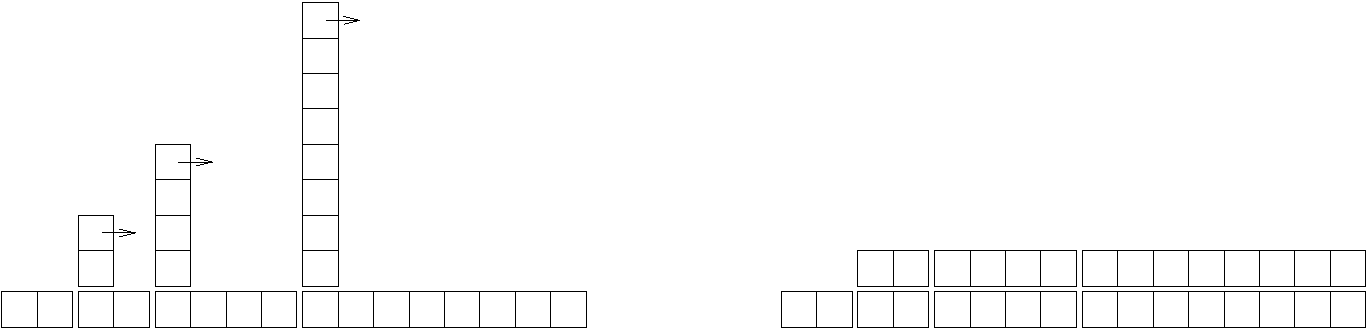
\includegraphics[scale=0.6]{figs/towers.pdf}}
\caption{Costo delle aggiunte a una Tabella Hash.\label{fig.hash}}
\end{figure}

Il lavoro supplementare di ricalcolo appare come una sequenza di torri sempre più alte e con spazi sempre più ampi tra due torri successive. Ora, se abbattete le torri, spalmando il costo del ridimensionamento su tutte le aggiunte, potete vedere graficamente che il costo del lavoro totale dopo $n$ aggiunte è $2n - 2$.

Una caratteristica importante di questo algoritmo è che quando ridimensioniamo la tabella hash, cresce geometricamente, cioè moltiplichiamo la dimensione per una costante. Se incrementaste le dimensioni aritmeticamente, aggiungendo ogni volta un numero fisso, il tempo medio per aggiunta sarebbe lineare.
\index{ridimensionamento geometrico}

Potete scaricare la mia implementazione di MappaHash da
\url{http://thinkpython2/code/Map.py}, ma ricordate che non c'è alcuna buona ragione per usarla. Piuttosto, se dovete fare una mappatura, usate un dizionario di Python.

\section{Glossario}

\begin{description}

\item[analisi degli algoritmi:] Un modo di confrontare gli algoritmi in termini di tempo di esecuzione e/o requisiti di memoria.
\index{analisi degli algoritmi}

\item[modello di macchina:] Rappresentazione semplificata di un computer usato per analizzare il comportamento degli algoritmi.
\index{modello di macchina}

\item[caso peggiore:] L'input che, con riferimento ad un algoritmo, lo rende più lento nell'esecuzione o richiede più spazio di memoria.
\index{caso peggiore}

\item[operazione dominante:] In un polinomio, il termine con il più alto esponente.
\index{operazione dominante}

\item[punto di intersezione:] La dimensione del problema per cui due diversi algoritmi richiedono lo stesso tempo di esecuzione o lo stesso spazio di memoria.
\index{intersezione, punto di}

\item[ordine di complessità:] Insieme di funzioni che, per gli scopi dell'analisi degli algoritmi, crescono in maniera equivalente. Per esempio, tutte le funzioni con incremento lineare appartengono allo stesso ordine di complessità.
\index{complessità, ordine di}

\item[Notazione O-grande:] Notazione per rappresentare l'ordine di complessità;
ad esempio, $O(n)$ rappresenta l'insieme delle funzioni con incremento lineare.
\index{Big-Oh notation}

\item[lineare:] Un algoritmo il cui tempo di esecuzione è proporzionale alle dimensioni del problema, almeno per i problemi di grandi dimensioni.
\index{lineare}

\item[quadratico:] Un algoritmo il cui tempo di esecuzione è proporzionale a
$n^2$, dove $n$ è una misura delle dimensioni del problema.
\index{quadratico}

\item[ricerca:] Il problema di rintracciare un elemento in un insieme (come una lista o un dizionario) oppure stabilire che non è presente.
\index{ricerca}

\item[tabella hash:] Struttura di dati che rappresenta una raccolta di coppie chiave-valore e ne esegue la ricerca a tempo costante.
\index{tabella hash}

\end{description}

\printindex

\clearemptydoublepage
%\blankpage
%\blankpage
%\blankpage


\end{document}
